%Version 3 December 2023
% See section 11 of the User Manual for version history
%
%%%%%%%%%%%%%%%%%%%%%%%%%%%%%%%%%%%%%%%%%%%%%%%%%%%%%%%%%%%%%%%%%%%%%%
%%                                                                 %%
%% Please do not use \input{...} to include other tex files.       %%
%% Submit your LaTeX manuscript as one .tex document.              %%
%%                                                                 %%
%% All additional figures and files should be attached             %%
%% separately and not embedded in the \TeX\ document itself.       %%
%%                                                                 %%
%%%%%%%%%%%%%%%%%%%%%%%%%%%%%%%%%%%%%%%%%%%%%%%%%%%%%%%%%%%%%%%%%%%%%

%%\documentclass[referee,sn-basic]{sn-jnl}% referee option is meant for double line spacing

%%=======================================================%%
%% to print line numbers in the margin use lineno option %%
%%=======================================================%%

%%\documentclass[lineno,sn-basic]{sn-jnl}% Basic Springer Nature Reference Style/Chemistry Reference Style

%%======================================================%%
%% to compile with pdflatex/xelatex use pdflatex option %%
%%======================================================%%

%%\documentclass[pdflatex,sn-basic]{sn-jnl}% Basic Springer Nature Reference Style/Chemistry Reference Style


%%Note: the following reference styles support Namedate and Numbered referencing. By default the style follows the most common style. To switch between the options you can add or remove “Numbered” in the optional parenthesis. 
%%The option is available for: sn-basic.bst, sn-vancouver.bst, sn-chicago.bst%  
 
%%\documentclass[pdflatex,sn-nature]{sn-jnl}% Style for submissions to Nature Portfolio journals
%%\documentclass[pdflatex,sn-basic]{sn-jnl}% Basic Springer Nature Reference Style/Chemistry Reference Style
\documentclass[pdflatex,sn-mathphys-num]{sn-jnl}% Math and Physical Sciences Numbered Reference Style 
%%\documentclass[pdflatex,sn-mathphys-ay]{sn-jnl}% Math and Physical Sciences Author Year Reference Style
%%\documentclass[pdflatex,sn-aps]{sn-jnl}% American Physical Society (APS) Reference Style
%%\documentclass[pdflatex,sn-vancouver,Numbered]{sn-jnl}% Vancouver Reference Style
%%\documentclass[pdflatex,sn-apa]{sn-jnl}% APA Reference Style 
%%\documentclass[pdflatex,sn-chicago]{sn-jnl}% Chicago-based Humanities Reference Style

%%%% Standard Packages
%%<additional latex packages if required can be included here>


\usepackage{algorithm}
\usepackage{algorithmic}

\usepackage{stmaryrd}

\usepackage{booktabs}
\usepackage{subcaption}
\usepackage{wrapfig}

\usepackage{float}
\usepackage{setspace}
\usepackage{makecell}

\usepackage{tikz}
\usepackage{pgfplots}
\usepackage{tikzscale}

\usepackage{graphicx}%
\usepackage{multirow}%
\usepackage{amsmath,amssymb,amsfonts}%
\usepackage{amsthm}%
\usepackage{mathrsfs}%
\usepackage[title]{appendix}%
\usepackage{xcolor}%
\usepackage{textcomp}%
\usepackage{manyfoot}%
% \usepackage{booktabs}%
% \usepackage{algorithm}%
% \usepackage{algorithmicx}%
% \usepackage{algpseudocode}%
\usepackage{listings}%
%%%%

%%%%%=============================================================================%%%%
%%%%  Remarks: This template is provided to aid authors with the preparation
%%%%  of original research articles intended for submission to journals published 
%%%%  by Springer Nature. The guidance has been prepared in partnership with 
%%%%  production teams to conform to Springer Nature technical requirements. 
%%%%  Editorial and presentation requirements differ among journal portfolios and 
%%%%  research disciplines. You may find sections in this template are irrelevant 
%%%%  to your work and are empowered to omit any such section if allowed by the 
%%%%  journal you intend to submit to. The submission guidelines and policies 
%%%%  of the journal take precedence. A detailed User Manual is available in the 
%%%%  template package for technical guidance.
%%%%%=============================================================================%%%%

%% as per the requirement new theorem styles can be included as shown below
\theoremstyle{thmstyleone}%
\newtheorem{theorem}{Theorem}%  meant for continuous numbers
%%\newtheorem{theorem}{Theorem}[section]% meant for sectionwise numbers
%% optional argument [theorem] produces theorem numbering sequence instead of independent numbers for Proposition
\newtheorem{proposition}[theorem]{Proposition}% 
%%\newtheorem{proposition}{Proposition}% to get separate numbers for theorem and proposition etc.

\theoremstyle{thmstyletwo}%
\newtheorem{example}{Example}%
\newtheorem{remark}{Remark}%

\theoremstyle{thmstylethree}%
\newtheorem{definition}{Definition}%

\raggedbottom
%%\unnumbered% uncomment this for unnumbered level heads

\usetikzlibrary{positioning, arrows}
\newcommand\subsetsim{\mathrel{\substack{
  \textstyle\subset\\[-0.2ex]\textstyle\sim}}}



\usepackage{lineno} 

\begin{document} %\linenumbers


\title[Article Title]{Article Title}

%%=============================================================%%
%% GivenName	-> \fnm{Joergen W.}
%% Particle	-> \spfx{van der} -> surname prefix
%% FamilyName	-> \sur{Ploeg}
%% Suffix	-> \sfx{IV}
%% \author*[1,2]{\fnm{Joergen W.} \spfx{van der} \sur{Ploeg} 
%%  \sfx{IV}}\email{iauthor@gmail.com}
%%=============================================================%%

\author*[1,2]{\fnm{First} \sur{Author}}\email{iauthor@gmail.com}

\author[2,3]{\fnm{Second} \sur{Author}}\email{iiauthor@gmail.com}
\equalcont{These authors contributed equally to this work.}

\author[1,2]{\fnm{Third} \sur{Author}}\email{iiiauthor@gmail.com}
\equalcont{These authors contributed equally to this work.}

\affil*[1]{\orgdiv{Department}, \orgname{Organization}, \orgaddress{\street{Street}, \city{City}, \postcode{100190}, \state{State}, \country{Country}}}

\affil[2]{\orgdiv{Department}, \orgname{Organization}, \orgaddress{\street{Street}, \city{City}, \postcode{10587}, \state{State}, \country{Country}}}

\affil[3]{\orgdiv{Department}, \orgname{Organization}, \orgaddress{\street{Street}, \city{City}, \postcode{610101}, \state{State}, \country{Country}}}

%%==================================%%
%% Sample for unstructured abstract %%
%%==================================%%

\abstract{Detecting structural anomalies in graphs is crucial to uncover unexpected patterns and mitigate risks in fields such as cybersecurity, social network analysis, and biological research. Existing methods, which often rely on machine learning approaches, struggle to balance detection effectiveness, scalability, and explainability.
In this paper, we introduce Minomaly, an unsupervised framework that combines subgraph mining with Graph Neural Networks (GNNs) to detect rare node neighborhoods indicative of structural anomalies. By embedding subgraphs into an Order Embedding Space (OES), Minomaly efficiently estimates subgraph frequencies and employs a greedy search algorithm to expand infrequent structures. This approach enables the detection of anomalies in a way that is both explainable and computationally efficient. Experiments on well-established benchmark datasets demonstrate that Minomaly consistently outperforms the state-of-the-art methods in detection quality and scalability, handling large graphs without memory overhead issues.\\ Our code will be available at \href{https://github.com/gbay7/minomaly}{https://github.com/gbay7/minomaly}.}

%%================================%%
%% Sample for structured abstract %%
%%================================%%

% \abstract{\textbf{Purpose:} The abstract serves both as a general introduction to the topic and as a brief, non-technical summary of the main results and their implications. The abstract must not include subheadings (unless expressly permitted in the journal's Instructions to Authors), equations or citations. As a guide the abstract should not exceed 200 words. Most journals do not set a hard limit however authors are advised to check the author instructions for the journal they are submitting to.
% 
% \textbf{Methods:} The abstract serves both as a general introduction to the topic and as a brief, non-technical summary of the main results and their implications. The abstract must not include subheadings (unless expressly permitted in the journal's Instructions to Authors), equations or citations. As a guide the abstract should not exceed 200 words. Most journals do not set a hard limit however authors are advised to check the author instructions for the journal they are submitting to.
% 
% \textbf{Results:} The abstract serves both as a general introduction to the topic and as a brief, non-technical summary of the main results and their implications. The abstract must not include subheadings (unless expressly permitted in the journal's Instructions to Authors), equations or citations. As a guide the abstract should not exceed 200 words. Most journals do not set a hard limit however authors are advised to check the author instructions for the journal they are submitting to.
% 
% \textbf{Conclusion:} The abstract serves both as a general introduction to the topic and as a brief, non-technical summary of the main results and their implications. The abstract must not include subheadings (unless expressly permitted in the journal's Instructions to Authors), equations or citations. As a guide the abstract should not exceed 200 words. Most journals do not set a hard limit however authors are advised to check the author instructions for the journal they are submitting to.}

\keywords{Graph Anomaly Detection, Unsupervised Learning, GNNs, Order Embedding}

%%\pacs[JEL Classification]{D8, H51}

%%\pacs[MSC Classification]{35A01, 65L10, 65L12, 65L20, 65L70}

\maketitle



\section{Introduction}
Graph Anomaly Detection (GAD) plays a crucial role in uncovering hidden insights and mitigating risks in various domains. For example, in cybersecurity, detecting anomalous network traffic patterns can help identify potential intrusions or malicious activities. In social network analysis, identifying anomalous behaviors can assist in detecting fake accounts, spam, or unusual communication patterns. Similarly, in biological networks, anomaly detection can highlight proteins or genes with unusual interactions, shedding light on disease mechanisms or novel biological processes \cite{akoglu2015graph,Ma_2023,Ruff_2021}.
%\begin{wrapfigure}{r}{0.4\textwidth}
%    \centering
%    \resizebox{\linewidth}{!}{\begin{tikzpicture}[
    normal_account/.style={circle, draw=black, fill=green!20, minimum size=0.5cm},
    gray_account/.style={circle, draw=black!40, fill=green!10, minimum size=0.5cm, opacity=0.5},
    suspicious_account/.style={circle, draw=red, thick, fill=red!10, minimum size=0.6cm},
    normal_transaction/.style={->, thick, black!70, >=stealth},
    gray_transaction/.style={->, thick, black!40, >=stealth, opacity=0.5},
    suspicious_transaction/.style={->, red!70, thick, >=stealth},
    suspicious_gray_transaction/.style={->, red!40, thick, >=stealth, opacity=0.5},
    internal_transaction/.style={-, red, thick, dashed, >=stealth},
    algorithm/.style={rectangle, rounded corners=3mm, draw=blue!60, fill=blue!5, 
                     minimum width=2.5cm, minimum height=2.5cm, align=center,
                     drop shadow},
    data_flow/.style={->, thick, blue!70, dashed, >=stealth},
    detection/.style={->, ultra thick, red!80, >=stealth},
    highlight/.style={draw=red, thick, dashed, rounded corners=2mm},
    pattern_dots/.style={circle, fill=black!70, inner sep=0.7pt}
]

% Define a background layer for highlighting
\pgfdeclarelayer{background}
\pgfsetlayers{background,main}

% Financial Network
\begin{scope}[local bounding box=network, shift={(-6,0)}]
    % Banks/Financial institutions with correctly oriented bank icons
    \node[inner sep=0] (bank1) at (-4,2) {  \begin{tikzpicture}[scale=0.03, line join=round, line cap=round]

    \fill[white, rounded corners=1pt] (-1.5,-1.35) rectangle (1.5,-1.28);

    % Triangle roof (flipped)
    \draw[draw=black!60, line width=0.9] (12,23) -- (23,18) -- (1,18) -- cycle;
    
    % Base line (flipped)
    \draw[black!60, line width=0.5] (1,1) -- (23,1);
    
    % Left column (flipped)
    \draw[draw=black!60, line width=0.9] (2,4) -- (2,15) -- (6,15) -- (6,4) -- cycle;
    
    % Right column (flipped)
    \draw[draw=black!60, line width=0.9] (18,4) -- (18,15) -- (22,15) -- (22,4) -- cycle;
    
    % Middle column (flipped)
    \draw[draw=black!60, line width=0.9] (10,4) -- (10,15) -- (14,15) -- (14,4) -- cycle;
  \end{tikzpicture}};
    \node[font=\scriptsize, above=0.1cm] at (bank1.north) {Bank 1};
    
    \node[inner sep=0] (bank2) at (0,2) {  
\begin{tikzpicture}[scale=0.03, line join=round, line cap=round]

    \fill[white, rounded corners=1pt] (-1.5,-1.35) rectangle (1.5,-1.28);

    % Triangle roof (flipped)
    \draw[draw=black!60, line width=0.9] (12,23) -- (23,18) -- (1,18) -- cycle;
    
    % Base line (flipped)
    \draw[black!60, line width=0.5] (1,1) -- (23,1);
    
    % Left column (flipped)
    \draw[draw=black!60, line width=0.9] (2,4) -- (2,15) -- (6,15) -- (6,4) -- cycle;
    
    % Right column (flipped)
    \draw[draw=black!60, line width=0.9] (18,4) -- (18,15) -- (22,15) -- (22,4) -- cycle;
    
    % Middle column (flipped)
    \draw[draw=black!60, line width=0.9] (10,4) -- (10,15) -- (14,15) -- (14,4) -- cycle;
  \end{tikzpicture}};
    \node[font=\scriptsize, above=0.1cm] at (bank2.north) {Bank 2};
    
    \node[inner sep=0, opacity=0.5] (bank3) at (4,2) {  
\begin{tikzpicture}[scale=0.03, line join=round, line cap=round]

    \fill[white, rounded corners=1pt] (-1.5,-1.35) rectangle (1.5,-1.28);

    % Triangle roof (flipped)
    \draw[draw=black!60, line width=0.9] (12,23) -- (23,18) -- (1,18) -- cycle;
    
    % Base line (flipped)
    \draw[black!60, line width=0.5] (1,1) -- (23,1);
    
    % Left column (flipped)
    \draw[draw=black!60, line width=0.9] (2,4) -- (2,15) -- (6,15) -- (6,4) -- cycle;
    
    % Right column (flipped)
    \draw[draw=black!60, line width=0.9] (18,4) -- (18,15) -- (22,15) -- (22,4) -- cycle;
    
    % Middle column (flipped)
    \draw[draw=black!60, line width=0.9] (10,4) -- (10,15) -- (14,15) -- (14,4) -- cycle;
  \end{tikzpicture}};
    \node[font=\scriptsize, above=0.1cm, opacity=0.5] at (bank3.north) {Bank $n$};
    
    % Normal accounts with smaller labels
    \node[normal_account, label={[font=\scriptsize]below:A1}] (a1) at (-5,0) {};
    \node[normal_account, label={[font=\scriptsize]below:A2}] (a2) at (-3.7,0) {};
    \node[normal_account, label={[font=\scriptsize]below:A3}] (a3) at (-1,0) {};
    \node[normal_account, label={[font=\scriptsize]below:A4}] (a4) at (1,0) {};
    \node[gray_account, label={[font=\scriptsize, opacity=0.5]below:}] (a5) at (3.7,0) {};
    \node[gray_account, label={[font=\scriptsize, opacity=0.5]below:}] (a6) at (5,0) {};
    
    % Suspicious accounts moved higher up in the diagram
    \node[suspicious_account, label=below:S1] (s1) at (-1,-2) {};
    \node[suspicious_account, label=below:S2] (s2) at (1,-2) {};
    \node[suspicious_account, label=left:S3] (s3) at (-2,-3) {};
    \node[suspicious_account, label=right:S4] (s4) at (2,-3) {};
    \node[suspicious_account, label=below:S5] (s5) at (0.6,-3.8) {};
    
    % Normal transactions
    \draw[normal_transaction] (a1) -- (bank1);
    \draw[normal_transaction] (bank1) -- (a2);
    \draw[normal_transaction] (a3) -- (bank2);
    \draw[normal_transaction] (bank2) -- (a4);
    \draw[gray_transaction] (a5) -- (bank3);
    \draw[gray_transaction] (bank3) -- (a6);
    \draw[normal_transaction] (bank1) -- (bank2);
    \draw[gray_transaction] (bank2) -- (bank3);
    
    % Add pattern dots to show frequent patterns
    \node[pattern_dots] at ($(bank2)!0.25!(bank3) + (0,0.3)$) {};
    \node[pattern_dots] at ($(bank2)!0.5!(bank3) + (0,0.3)$) {};
    \node[pattern_dots] at ($(bank2)!0.75!(bank3) + (0,0.3)$) {};
    
    % % For A1 to Bank1
    % \node[pattern_dots] at ($(a1)!0.25!(bank1) + (-0.2,0.2)$) {};
    % \node[pattern_dots] at ($(a1)!0.5!(bank1) + (-0.2,0.2)$) {};
    % \node[pattern_dots] at ($(a1)!0.75!(bank1) + (-0.2,0.2)$) {};
    
    % % For Bank2 to A4
    % \node[pattern_dots] at ($(bank2)!0.25!(a4) + (0.2,-0.2)$) {};
    % \node[pattern_dots] at ($(bank2)!0.5!(a4) + (0.2,-0.2)$) {};
    % \node[pattern_dots] at ($(bank2)!0.75!(a4) + (0.2,-0.2)$) {};

    % Suspicious accounts' transactions with banks
    \draw[suspicious_transaction] (s1) -- (bank1);
    \draw[suspicious_transaction] (bank2) -- (s2);
    \draw[suspicious_transaction] (s3) -- (bank1);
    \draw[suspicious_gray_transaction] (bank3) -- (s4);
    \draw[suspicious_transaction] (s5) -- (bank2);
    
    % Suspicious internal transactions (forming a clique)
    \draw[internal_transaction] (s1) to[bend left=20] (s2);
    \draw[internal_transaction] (s2) to[bend left=20] (s4);
    \draw[internal_transaction] (s4) to[bend left=20] (s5);
    \draw[internal_transaction] (s5) to[bend left=20] (s3);
    \draw[internal_transaction] (s3) to[bend left=20] (s1);
    \draw[internal_transaction] (s1) to[bend left=40] (s5);
    \draw[internal_transaction] (s2) to[bend left=40] (s3);
    \draw[internal_transaction] (s4) to[bend left=50] (s1);
    \draw[internal_transaction] (s2) to[bend left=40] (s5);
    \draw[internal_transaction] (s3) to[bend left=20] (s4);
    
\end{scope}

% Graph Anomaly Detection Algorithm - positioned to the right of the network
\node[algorithm] (algorithm) at (2,0) {
    \textbf{Node}\\
    \textbf{Anomaly}\\
    \textbf{Detection}
};

% Data flow from network to algorithm
\draw[data_flow] (network.east |- 0,1) to[bend right=10] (algorithm.west |- 0,0.5);
\draw[data_flow] (network.east |- 0,-1) to[bend left=10] (algorithm.west |- 0,-0.5);

% Detection results - use simple absolute positioning
\node[align=center] (result_label) at (5,0) {};

% Connect algorithm to results
\draw[detection] (algorithm.east) -- (result_label);

% Suspicious accounts arranged vertically
\node[suspicious_account, label=right:S1] (rs1) at (5.5,2) {};
\node[suspicious_account, label=right:S2] (rs2) at (5.5,1) {};
\node[suspicious_account, label=right:S3] (rs3) at (5.5,0) {};
\node[suspicious_account, label=right:S4] (rs4) at (5.5,-1) {};
\node[suspicious_account, label=right:S5] (rs5) at (5.5,-2) {};

% Highlight the suspicious accounts in the network
\begin{pgfonlayer}{background}
    \node[highlight, fit=(s1) (s2) (s3) (s4) (s5), inner sep=5pt] {};
    \node[draw=red!70, fill=white, align=center, font=\scriptsize, rounded corners=1mm] 
        at ($(s3) + (-1.5,-0.6)$) {Suspicious\\Clique};
\end{pgfonlayer}

% Legend - repositioned to the bottom
\matrix [
    draw,
    fill=white,
    below right=0.2cm and -5.1cm of network.south,
    matrix of nodes,
    nodes={font=\scriptsize},
    column 1/.style={nodes={scale=0.6, transform shape, anchor=center}},
    column 3/.style={nodes={scale=0.6, transform shape, anchor=center}},
    column 5/.style={nodes={scale=0.6, transform shape, anchor=center}},
    column 7/.style={nodes={scale=0.6, transform shape, anchor=center}},
    column 9/.style={nodes={scale=0.6, transform shape, anchor=center}},
    column 11/.style={nodes={scale=0.6, transform shape, anchor=center}},
    column 13/.style={nodes={scale=0.6, transform shape, anchor=center}},
    column 15/.style={nodes={scale=0.6, transform shape, anchor=center}},
    even column/.style={align=left, text width=1.2cm},
    column sep=0.05cm,
    inner sep=0.1cm,
    rounded corners
] {
    \node[scale=0.7] {  
\begin{tikzpicture}[scale=0.03, line join=round, line cap=round]

    \fill[white, rounded corners=1pt] (-1.5,-1.35) rectangle (1.5,-1.28);

    % Triangle roof (flipped)
    \draw[draw=black!60, line width=0.9] (12,23) -- (23,18) -- (1,18) -- cycle;
    
    % Base line (flipped)
    \draw[black!60, line width=0.5] (1,1) -- (23,1);
    
    % Left column (flipped)
    \draw[draw=black!60, line width=0.9] (2,4) -- (2,15) -- (6,15) -- (6,4) -- cycle;
    
    % Right column (flipped)
    \draw[draw=black!60, line width=0.9] (18,4) -- (18,15) -- (22,15) -- (22,4) -- cycle;
    
    % Middle column (flipped)
    \draw[draw=black!60, line width=0.9] (10,4) -- (10,15) -- (14,15) -- (14,4) -- cycle;
  \end{tikzpicture}}; & Financial Institution &
    \node[normal_account] {}; & Normal Account &
    \node[suspicious_account] {}; & Suspicious Account &
    \draw[normal_transaction] (-0.15,0) -- (0.15,0); & Normal Tx &
    \draw[suspicious_transaction] (-0.15,0) -- (0.15,0); & Suspicious Tx &
    \draw[internal_transaction] (-0.15,0) -- (0.15,0); & Money Flow 
    % &
    % \draw[data_flow] (-0.15,0) -- (0.15,0); & Data Flow &
    % \node[pattern_dots] {}; \node[pattern_dots] at (0.1,0) {}; \node[pattern_dots] at (0.2,0) {}; & Frequent Pattern 
    \\
};

\end{tikzpicture}}
%    \caption{\footnotesize Illustration of node anomaly detection.}
%    \label{fig:gad_concept}
%\end{wrapfigure}

Unsupervised node anomaly detection has gained significant research attention in recent years due to its wide applicability. In graph data, nodes are interconnected to form patterns. Nodes with attribute vectors that deviate considerably from the global attribute norm are often considered global anomalies. While node attributes provide valuable information, the edges between nodes offer additional insights. If a node belongs to an unusual connection pattern or neighborhood, all nodes within this structure are collectively anomalous and called structural anomalies. When node attributes are considered within this abnormal structure, these anomalies are referred to as contextual anomalies \cite{NEURIPS2022-acc1ec4a,Ma_2023}. Our primary focus, however, is on \textbf{structural anomalies}. While existing methods have advanced in detecting these anomalies, they often lack generality and interpretability. BOND \cite{NEURIPS2022-acc1ec4a} consider structural anomalies as densely connected nodes. However, in some real-world geometric graphs, dense connections are common, making this assumption inadequate. Other methods rely on specific motif distributions \cite{bandyopadhyay2020outlier,xu2022contrastive,yuan2024higherorder}, which limits their applicability to diverse real-world contexts such as fraud detection. Existing unsupervised deep learning techniques often lack solid explanations for their results, limiting their interpretability. Traditionally, frequent pattern outlier detection methods provided interpretable results but were computationally expensive due to the need to enumerate patterns and match similar ones \cite{bressan2021faster,he2004frequent,yan2002gspan}. This computational burden arises because the problem reduces to the subgraph isomorphism problem, which is NP-complete. In these methods, frequency serves as a measure of abnormality because rare structures are more likely to be anomalous.

To address these limitations, we propose \textbf{Minomaly}, an unsupervised, interpretable, and scalable framework for structural anomaly detection in graphs. Our approach proceeds in two distinct steps: \textbf{(a) \textit{Order Embedding Space (OES) construction}}  --- Minomaly combines subgraph mining with GNN-based order embeddings to encode graph neighborhoods efficiently. This step allows for accurate frequency estimation of subgraphs; \textbf{(b) \textit{Anomalous structures search}}  --- Using the geometrical properties of the OES, Minomaly employs a novel greedy search algorithm to identify rare and unusual node structures, allowing interpretable anomaly detection;
% \textcolor{blue}{
% Experiments on benchmark datasets validate the effectiveness of Minomaly, demonstrating its superior performance compared to existing methods in both detection accuracy and scalability.
% }
Our contributions can be summarized as follows:
\begin{itemize}
    \item A new formalization of structural anomaly detection in graphs using subgraph mining. A proof of the correctness of the counting measure used to enumerate anomalous subgraphs, based on the anti-monotonicity property, is provided. Additionally, a generalized definition of structural node anomaly detection is proposed to support anomaly detection across multiple contexts.
    \item A novel application of order embeddings to graph anomaly detection. Minomaly leverages GNN order embeddings to efficiently encode graph structures.
    \item A new optimization technique in anomalous structures search by exploiting the geometrical properties of the OES which significantly reduces the number of nodes that need to be verified during the search for anomalous structures.
    \item A novel, computationally efficient greedy search algorithm for identifying and interpreting unusual structures in graphs, enabling explainable GAD.
    \item An in-depth experimental study on widely used benchmark datasets to validate Minomaly's performance. 
    % Our results demonstrate superior detection accuracy and scalability compared to state-of-the-art methods.
\end{itemize}

The rest of this paper is organized as follows:  
{Section~\ref{sec:relatedworks}} introduces the  related works. {Section~\ref{sec:problem}} formalizes the problem of anomaly detection in graphs and provides a proof of the use of subgraph mining for structural anomaly detection.  
{Section~\ref{sec:proposal}} presents the Minomaly framework in detail.  
{Section~\ref{sec:eval}} discusses our experimental results and compares them with existing approaches. Finally, {Section~\ref{sec:conclusion}} concludes the paper and outlines future research directions.

\section{Related Work}
\label{sec:relatedworks}

Non-deep learning approaches to node anomaly detection often utilize matrix decomposition techniques, such as Radar \cite{li2017radar} and ANOMALOUS \cite{peng2018anomalous}, clustering methods like SCAN \cite{xu2007scan}, and pattern mining approaches like PANG \cite{potin2023pattern}. Recently, deep learning methods leveraging the representation power of GNNs have been proposed. For instance, DOMINANT \cite{ding2019deep} uses a GCN encoder and two decoders for structural and attribute reconstruction, while AnomalyDAE \cite{fan2020anomalydae} employs two separate autoencoders (AEs) and combines their reconstruction losses for anomaly scoring. DONE \cite{bandyopadhyay2020outlier} introduces structural and attribute AEs with MLP-based encoders and decoders to reconstruct adjacency and node attribute matrices, and AdONE \cite{bandyopadhyay2020outlier} extends DONE with adversarial learning. CONAD \cite{xu2022contrastive} uses contrastive learning based on human prior knowledge of structural and contextual anomalies. However, none of these deep learning methods have been evaluated on large graphs or focused on metrics other than AUC in their studies.

Focusing directly on node-level graph anomaly detection using deep learning presents challenges. Reconstruction methods \cite{ding2019deep,fan2020anomalydae,xu2022contrastive,yuan2024higherorder} aim to learn the global behavior of node information and intentionally miss rare patterns to produce high reconstruction errors for these patterns. However, this approach may fail \cite{Ruff_2021} because the balance between learning normal and abnormal patterns is neither well-controlled nor interpretable. To address this, we utilize deep learning specifically for subgraph matching, which deals with generalized, class-balanced ground truth, as in NeuroMatch \cite{rex2020neural}.

A few graph outlier detection methods have relied on pattern mining approaches \cite{potin2023pattern,yuan2024higherorder}, but they still face the same computational issues. The NeuroMatch method for subgraph matching, inspired by \cite{vendrov2016orderembeddings}, provides an approximate frequency count of graph neighborhoods using GNN. SPMiner for frequent subgraph mining \cite{ying2024representation} relies on NeuroMatch for order embedding. Although SPMiner was successful in identifying most small frequent motifs, it lacked accuracy in predicting graph-level frequency. To address the limitations of existing GAD approaches, we leverage subgraph mining and GNN-based order embeddings to detect and interpret rare node neighborhoods in graphs.

%In order to address  limitations of GAD existing approaches, we propose to combining subgraph mining with GNN-based order embeddings to detect and interpret rare node neighborhoods in graphs.

\section{Problem Definition}
\label{sec:problem}
A static directed graph $G = (V, E)$ consists of a fixed set of nodes $V$, and edges $E \subseteq V \times V$ which represent the connections between nodes.
The order of $G$ is its number of vertices $|V|$, and its size is its number of edges $|E|$.

\paragraph{Induced Subgraph}
Let $S \subseteq V$. The induced subgraph $G[S]$ in $G$ by $S$ is the graph $G[S] = (S, E_S)$, where $E_S = \{(u, v) \in E \mid u, v \in S\}$, the set of edges from $G$ that connect two nodes in $S$. We write $G' \subseteq G$ if $G'$ is subgraph of $G$, and $\mathcal{G}(G)$ the set of subgraphs of $G$.

\paragraph{Anchor Node}
Let $u \in V$. The \textbf{anchor node} is a special node from which the subgraph is defined. The \textbf{structure graph} or \textbf{neighborhood graph} of the node $u$ is the connected subgraph induced by the set of nodes that are reachable from $u$, including $u$ itself. This subgraph serves as the basis for graph embedding and comparison in subgraph matching.

\paragraph{Isomorphism}
Let $G[S], G[T] \in \mathcal{G}(G)$. We say $G[S]$ and $G[T]$ are isomorphic, denoted $G[S] \cong G[T]$, if and only if:
\[\footnotesize
\begin{cases}
    \exists f: S \to T, \; f \text{ is bijective}, \\
    \forall u_1, u_2 \in S: (u_1, u_2) \in E_S \iff (f(u_1), f(u_2)) \in E_T.
\end{cases}
\]

\paragraph{Order Embedding Function}
An \textbf{order embedding} function for graphs, denoted as $\phi:\mathcal{G}(G) \to \mathbb{R}^d$, is an injective function that maps a subgraph of $G$ into a $d$-dimensional embedding space such that for two subgraphs $G_1, G_2 \in \mathcal{G}(G)$:
\[
G_1 \subsetsim G_2 \iff \phi(G_1) \preceq \phi(G_2), \quad 
\text{\footnotesize such that $G_1 \subsetsim G_2$  means $\exists G_{iso} \subseteq G_2 : G_{iso} \cong G_1$}
\]
Here, the partial order $\preceq$ on the embedding space is defined component-wise, meaning $\phi(G_1) \preceq \phi(G_2)$ if and only if $\phi_i(G_1) \leq \phi_i(G_2), \forall i \in \llbracket 1, d \rrbracket$ such that $\phi = (\phi_1, \phi_2, \dots, \phi_d)$. The partial order $\subsetsim$ on $\mathcal{G}(G)$ denotes subgraph isomorphism.

\paragraph{Structural Anomaly}
Let $u \in V$. The node $u$ is a \textbf{structural anomaly} of $G$ if and only if $u$ belongs to an unexpected structure graph of $u$.
\begin{itemize}
 \item We define unexpected graph $G'$ in $G$, as rare subgraph in term of graph frequency $freq_G: \mathcal{G}(G) \to \mathbb{N} $ that quantifies the existence of its similar (isomorphic) subgraphs in $G$
 \[
  freq_G(G') < T_F \quad \text{with} \quad T_F > 0
 \]
 \item All nodes of the graph $G'$ are structural anomalies.
\end{itemize}

\paragraph{Anti-monotonicity counting property}
$freq_G$ is anti-monotonic, if for all $G_1, G_2$ subgraphs of $G$. \[G_1 \subseteq G_2 \implies freq_G(G_2) \le freq_G(G_1)\]

This implies that the frequency of a graph is never greater than the frequency of any of its subgraphs. Consequently, if a graph is infrequent, all graphs containing it are also infrequent. The correctness of the counting measure is typically evaluated through the anti-monotonicity property \cite{calders2008anti}. 

\paragraph{Frequency Measure}
For any $G' \in \mathcal{G}(G)$, we define:
\[ \footnotesize
\begin{cases}
    UP_G(G') &= \{G_{up} \subseteq G \mid \exists G_{iso} \subseteq G_{up}: G_{iso} \cong G'\} \\ &= \{G_{up} \subseteq G \mid \phi(G') \preceq \phi(G_{up})\}, \\
    Freq_G(G') &= |UP_G(G')|.
\end{cases}
\]

Our approach relies on an estimation of the frequency measure \( Freq_G \), defined as the number of graphs that contain a matching of \( G' \). In the following, we prove the anti-monotonicity of $Freq_G$:

\begin{proof}
Let $G_1, G_2 \in \mathcal{G}(G)$ such that $G_1=(S_1, E_1)$, $G_2=(S_2, E_2)$ and $G_1 \subseteq G_2$.  
\begin{itemize}
    \item If $G_{up} \in UP_G(G_2)$, then $\exists G_{iso} \subseteq G_{up}$ such that $G_{iso} \cong G_2$. 
    \item Since $G_1 \subseteq G_2$, $\exists G_{iso}' \subseteq G_{iso} \subseteq G_{up}$ such that $G_{iso}' \cong G_1$ (by restricting $f$ to $S_1 \subseteq S_2$). 
    \item Thus, $G_{up} \in UP_G(G_1)$, and we have $UP_G(G_2) \subseteq UP_G(G_1)$. 
\end{itemize}
Taking cardinalities: $|UP_G(G_2)| \leq |UP_G(G_1)|$ i.e. $Freq_G(G_2) \leq Freq_G(G_1)$, therefore, $Freq_G$ is anti-monotonic.
\end{proof}


%In this framework, the anchor node $u$ plays a central role in defining and embedding subgraphs, as the neighborhood graph $G[N(u)]$ is embedded and compared using the order embedding $\phi$. This allows for effective subgraph matching by comparing the embeddings of neighborhood graphs centered at anchor nodes.

% \vspace*{-15pt}
\section{Proposed Method: Minomaly}
\label{sec:proposal}

In this section, we present \textbf{Minomaly}, an approach that uses a GNN for the detection of Structural Anomalies in graphs. Minomaly employs the \text{NeuroMatch} method \cite{rex2020neural} inspired by \cite{vendrov2016orderembeddings} to embed graph structures into an Order Embedding Space (OES). This embedding provides an approximate frequency count of small structural neighborhood graphs of nodes.

We introduce a greedy search method to expand infrequent neighboring graphs using OES. Graph patterns that meet a certain frequency threshold are identified as structural anomalies. The resulting graph represents the structural anomalies, demonstrating the interpretability of the method. Also, it applies a heuristic search to select potential node anchors from  the embedded space that produce anomalous patterns, rather than verifying the normality of all nodes in the graph.

%In comparison to existing non-interpretable deep learning methods, Minomaly demonstrates superior performance across all measures of the binary classification, particularly in terms of the area under ROC (AUC), Average Precision (AP), Recall, and Precision.
% \vspace*{-15pt}
\subsection{Order Embedding}
% \vspace*{-5pt}
The primary function of the Order Embedding is to identify whether a given graph is a subgraph of another, and to quantify its frequency in the whole graph. For this purpose, as illustrated in Figure~\ref{fig:encoder_process}, it breaks down the graph $G$ into random subgraphs $RG=\{G'_1, G'_2, \dots, G'_k\}$ of different sizes from \texttt{min\_neigh\_size} to \texttt{max\_neigh\_size}, $k$ must be sufficiently large. These subgraphs are then processed through a GNN to generate their respective order embeddings in order to construct the Order Embedding Space (OES) that is used for counting subgraph occurrences. We have used the same architecture that is used for SPMiner Encoder \cite{ying2024representation} and synthetic data for training it. 
\vspace*{-13pt}
\begin{figure}[H]
    \centering
    % \hspace*{0.3cm}
    \resizebox{0.73\linewidth}{!}{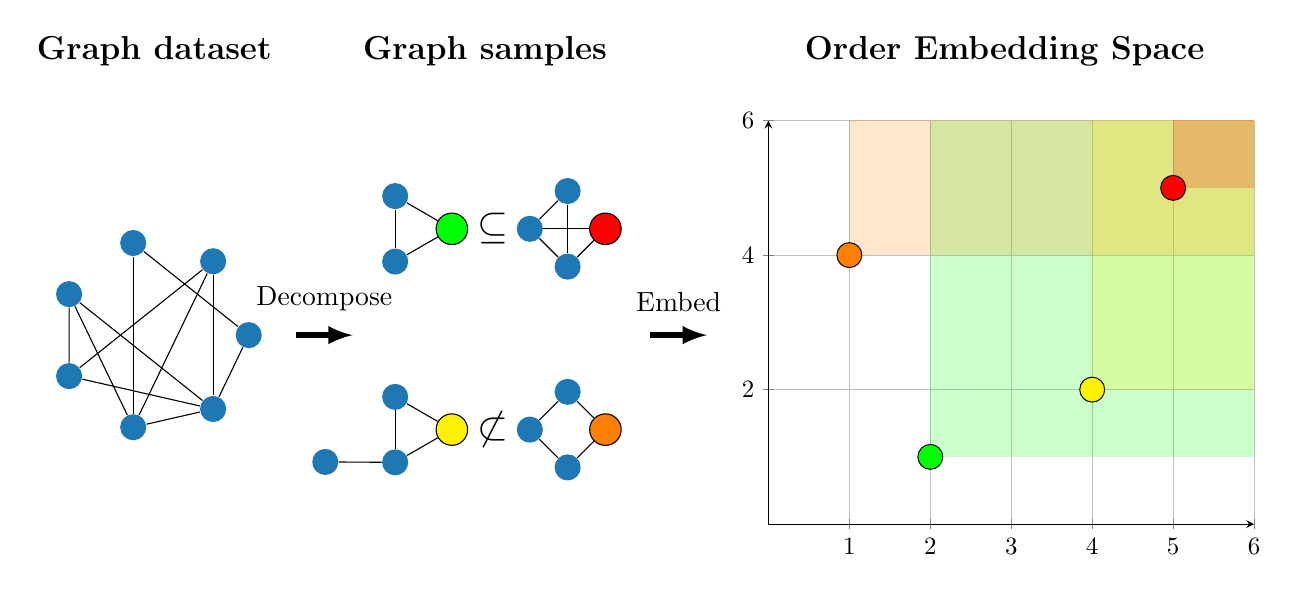
\begin{tikzpicture}[scale=0.6]
    \node at (-0.5, 6) {\large \textbf{Graph dataset}};
    \begin{scope}[shift={(-0.5,0)}]
      \draw
        (0.0:2) node[fill={rgb,255:red,31;green,119;blue,180}, minimum size=2mm, circle] (0){}
        (51.429:2) node[fill={rgb,255:red,31;green,119;blue,180}, minimum size=2mm, circle] (1){}
        (102.857:2) node[fill={rgb,255:red,31;green,119;blue,180}, minimum size=2mm, circle] (2){}
        (154.286:2) node[fill={rgb,255:red,31;green,119;blue,180}, minimum size=2mm, circle] (3){}
        (205.714:2) node[fill={rgb,255:red,31;green,119;blue,180}, minimum size=2mm, circle] (4){}
        (257.143:2) node[fill={rgb,255:red,31;green,119;blue,180}, minimum size=2mm, circle] (5){}
        (308.571:2) node[fill={rgb,255:red,31;green,119;blue,180}, minimum size=2mm, circle] (6){};
      \begin{scope}[-]
        \draw (0) to (2);
        \draw (0) to (6);
        \draw (1) to (4);
        \draw (1) to (5);
        \draw (1) to (6);
        \draw (2) to (5);
        \draw (3) to (4);
        \draw (3) to (5);
        \draw (3) to (6);
        \draw (4) to (6);
        \draw (5) to (6);
      \end{scope}
    \end{scope}
    \node at (6.5, 6) {\large \textbf{Graph samples}};
    \begin{scope}[shift={(2.5,0)}, scale=0.4]
      \draw[->, >=latex, line width=2pt] (0,0) --  node[label= above:Decompose] {} (3,0);
    \end{scope}
    
    \begin{scope}[shift={(8.25,2.25)}, scale=0.4]
      \draw
        (0.0:2) node[fill=red, minimum size=4mm, circle, draw, label] (1){}
        (90.0:2) node[fill={rgb,255:red,31;green,119;blue,180}, minimum size=2mm, circle] (3){}
        (180.0:2) node[fill={rgb,255:red,31;green,119;blue,180}, minimum size=2mm, circle] (4){}
        (270.0:2) node[fill={rgb,255:red,31;green,119;blue,180}, minimum size=2mm, circle] (6){};
      \begin{scope}[-]
        \draw (1) to (4);
        \draw (1) to (6);
        \draw (3) to (4);
        \draw (3) to (6);
        \draw (4) to (6);
      \end{scope}
    \end{scope}
    \begin{scope}[shift={(5,2.25)}, scale=0.4]
      \draw
        (0.0:2) node[fill=green, minimum size=4mm, circle, draw, label=right:\textbf{\Large $\subseteq$}] (1){}
        (120.0:2) node[fill={rgb,255:red,31;green,119;blue,180}, minimum size=2mm, circle] (4){}
        (240.0:2) node[fill={rgb,255:red,31;green,119;blue,180}, minimum size=2mm, circle] (6){};
      \begin{scope}[-]
        \draw (1) to (4);
        \draw (1) to (6);
        \draw (4) to (6);
      \end{scope}
    \end{scope}
    \begin{scope}[shift={(8.25,-2)}, scale=0.4]
      \draw
        (0.0:2) node[fill=orange, minimum size=4mm, circle, draw] (0){}
        (90.0:2) node[fill={rgb,255:red,31;green,119;blue,180}, minimum size=2mm, circle] (2){}
        (180.0:2) node[fill={rgb,255:red,31;green,119;blue,180}, minimum size=2mm, circle] (5){}
        (270.0:2) node[fill={rgb,255:red,31;green,119;blue,180}, minimum size=2mm, circle] (6){};
      \begin{scope}[-]
        \draw (0) to (2);
        \draw (0) to (6);
        \draw (2) to (5);
        \draw (5) to (6);
      \end{scope}
    \end{scope}
    \begin{scope}[shift={(5,-2)}, scale=0.4]
      \draw
        (0.0:2) node[fill=yellow, minimum size=4mm, circle, draw, label=right:{\textbf{\Large$\not\subset$}}] (1){}
        (120.0:2) node[fill={rgb,255:red,31;green,119;blue,180}, minimum size=2mm, circle] (4){}
        (240.0:2) node[fill={rgb,255:red,31;green,119;blue,180}, minimum size=2mm, circle] (6){}
        (200.0:5) node[fill={rgb,255:red,31;green,119;blue,180}, minimum size=2mm, circle] (7){};
      \begin{scope}[-]
        \draw (1) to (4);
        \draw (1) to (6);
        \draw (4) to (6);
        \draw (6) to (7);
      \end{scope}
    \end{scope}
    \begin{scope}[shift={(10,0)}, scale=0.4]
      \draw[->, >=latex, line width=2pt] (0,0) --  node[label= above:Embed] {} (3,0);
    \end{scope}
    \node at (17.5, 6) {\large \textbf{Order Embedding Space}};
    \begin{scope}[shift={(12.5,-4)}, scale=1.5]
        \begin{axis}[
            xmin=0, xmax=6,
            ymin=0, ymax=6,
            axis lines=center,
            grid=major,
        ]
                  
        % Shaded rectangular region for the red point
        \fill[green, opacity=0.2] (axis cs:2,1) rectangle (rel axis cs:2,1);
        
        % Shaded rectangular region for the red point
        \fill[orange, opacity=0.2] (axis cs:1,4) rectangle (rel axis cs:1,4);
        
        \fill[yellow, opacity=0.2] (axis cs:4,2) rectangle (rel axis cs:4,2);

        \fill[red, opacity=0.2] (axis cs:5,5) rectangle (rel axis cs:5,5);


        % Four points with big markers and labels
        \addplot[only marks, mark size=5pt, green, draw=black] coordinates {(2,1)};
        \node[red] at (axis cs:2,1) [above right] {};
        
        \addplot[only marks, mark size=5pt, orange, draw=black] coordinates {(1,4)};
        \node[orange] at (axis cs:1,4) [above right] {};
        
        \addplot[only marks, mark size=5pt, yellow, draw=black] coordinates {(4,2)};
        \node[blue] at (axis cs:5,2) [above right] {};
        
        \addplot[only marks, mark size=5pt, red, draw=black] coordinates {(5,5)};
        \node[orange] at (axis cs:4,5) [above right] {};
        
        \end{axis}     
    \end{scope}
  \end{tikzpicture}}
    \caption{\footnotesize Order Embedding Space construction process}
    \label{fig:encoder_process}
\end{figure}

This approach of subgraph matching is considered advantageous for these reasons:
\textbf{(a) \textit{Generalizability}} --- NeuroMatch shows the generalization test performance of subgraph matching across real-world datasets, by training only on a synthetic dataset. On the other hand, the model only handles subgraph matching without considering features;
\textbf{(b) \textit{OES geometric properties}} --- Using the partial order properties of the embeddings, the frequency of a subgraph $G'$ can be quantified by counting the upper-right embeddings of $RG$ graphs. Additionally, the anti-monotonicity property can be verified by how the space is organized according to graph size and order.
% \vspace*{-20pt}
\paragraph{Network Architecture}
The network employs GNN with a multi-layer perceptron (MLP) for binary classification (\( G_1 \subseteq G_2 \)). It takes two graphs, \( G_1 \) and \( G_2 \), as inputs. The model processes the graph structure through 8 layers of GraphSAGE-based graph convolutions with learnable skip connections \cite{hamilton2018inductive}. A post-processing layer with linear transformations and Leaky ReLU activations produces the embeddings \( \phi(G_1) \) and \( \phi(G_2) \). These embeddings are concatenated and passed through an MLP to generate the output.


\paragraph{Training goal}
The goal is to train the network to learn an order
embedding function $\phi$ that respects to its definition.

\paragraph{Train data}
To train the model, a set of positive and negative training instances are generated. For positive examples, we sample random subgraphs \( G^+_1 \) and \( G^+_2 \) from the graph \( G \) such that \( G^+_1 \subseteq G^+_2 \). For negative examples, we add enough random nodes or edges to a subgraph \( G^-_1 \) to generate $G^-_2$, or we can use any other valid random generation.

\paragraph{Loss function}
The learning penalty proposed by \cite{ying2024representation} is adopted and defined as
\begin{equation}
E(G_1, G_2) = \|\max(0, \phi(G_1) - \phi(G_2))\|^2
\end{equation}
The total hinge loss is then given by:
\begin{equation}
\sum_{(G^+_1, G^+_2) \in \text{Positives}} E(G^+_1, G^+_2) + \sum_{\left(G^-_1, G^-_2\right) \in \text{Negatives}} \max \left(0, \alpha - E\left(G^-_1, G^-_2\right)\right)
\end{equation}
where \(\alpha\) is the margin hyperparameter which controls the separation between penalties of positive and negative examples.

Consequently, for positive pairs \( G^+_1 \subseteq G^+_2 \), the embeddings are trained to satisfy \( \phi(G^+_1) \preceq \phi(G^+_2) \), as the penalty \( E(G^+_1, G^+_2) \) will be zero with proper learning and large in order to be minimized during training. For negative pairs \( G^-_1 \) and \( G^-_2 \), the violation \( E(G^-_1, G^-_2) \) is trained to be at least \( \alpha \), ensuring separation from positive pairs and minimizing the overall loss.

\begin{wrapfigure}[10]{r}{0.33\textwidth}
    \centering
    \vspace{-3pt}
    \resizebox{\linewidth}{!}{\input{figs/decoder/tex_oes_count}}
    \caption{\footnotesize Geometric visualization of the count prediction procedure in the OES}
    \label{fig:count_pred}
\end{wrapfigure}

\paragraph{Count prediction $Freq_G$}
To determine the frequency of a subgraph \( G' \), $Freq_G(G')$, we count the number of the random embedded subgraph \( G'_i \) from $RG=\{G'_1, G'_2, \dots, G'_k\}$ in the space, where \( \phi(G') \preceq \phi(G_i') \) as predicted by the network's output layer.
\textbf{\[Freq_G(G')=\frac{|\{G'_i \in RG \mid \phi(G') \preceq \phi(G'_i)\}|}{k}\]}
The $\phi(G'_i)$s are also the upper-rights points of $\phi(G')$ in the geometric space OES (see Figure \ref{fig:count_pred}).

\paragraph{Anti-monotonicity preservation}
As shown in Figure \ref{fig:embs_neighs_size}, the model organizes the space based on subgraph size (number of edges) and order (number of nodes), since larger graphs cannot be subgraphs of smaller ones. This indicates that $Freq_G$ is anti-monotonic, which supports its correctness.
\vspace*{-15pt}
\begin{figure}[H]
    \centering
    \begin{subfigure}{0.65\textwidth}
        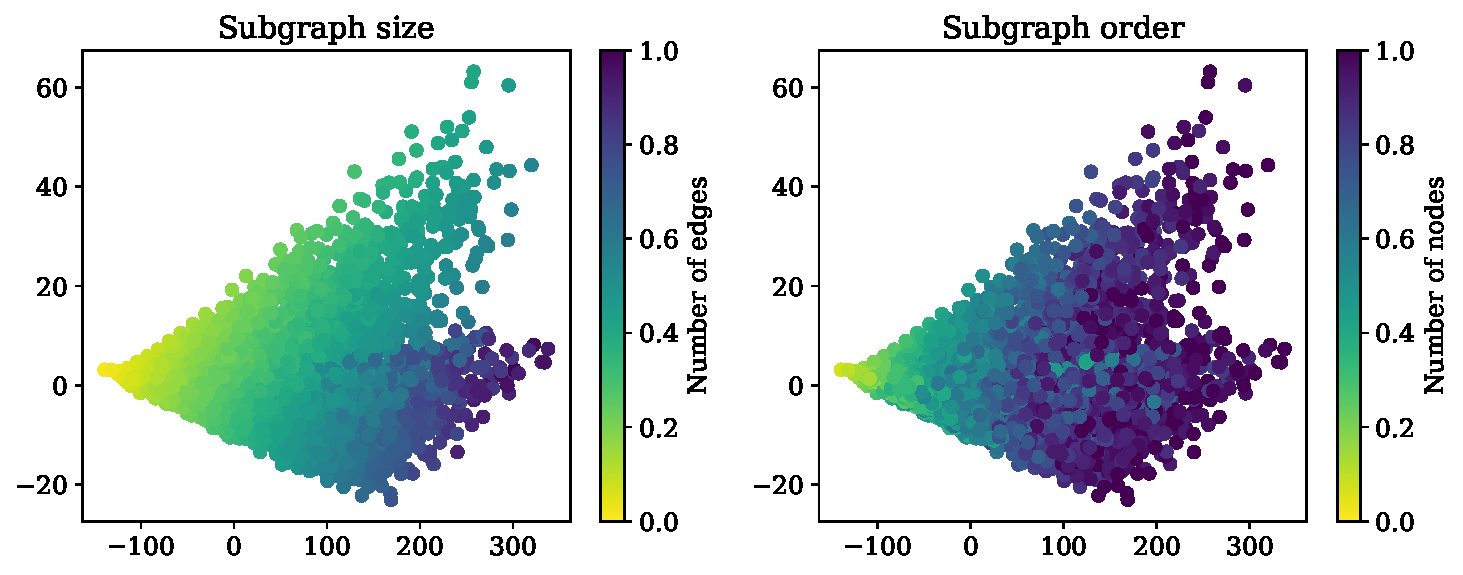
\includegraphics[width=\textwidth]{figs/pca_emb_c.pdf}
        \caption{\footnotesize PCA-based visualization}
        \label{fig:pca_embs}
    \end{subfigure}
    \begin{subfigure}{0.3\textwidth}
        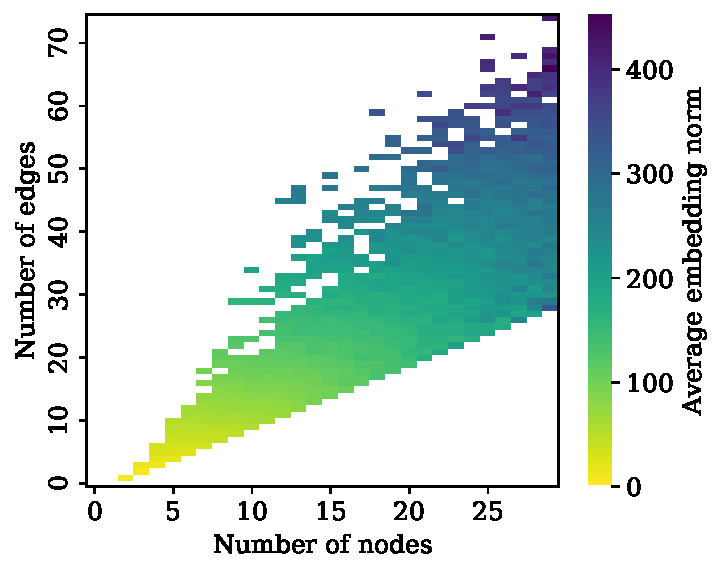
\includegraphics[width=\textwidth]{figs/heatmap.pdf}
        \caption{\footnotesize Heatmap}
        \label{fig:heatmap}
    \end{subfigure}
    \caption{\footnotesize (a) PCA visualization of order embeddings for random neighborhoods of 1–30 nodes from the Cora dataset. PCA preserves straight lines, indicating subgraph containment of a point lies within a quadrilateral region \cite{ying2024representation}. (b) The Heatmap shows average embedding norms by graph size and order, highlighting structure-embedding relationships. Lighter shades for smaller graphs, darker for larger ones by size or order.}
    \label{fig:embs_neighs_size}
\end{figure}
% \vspace*{-60pt}
\vspace*{-30pt}
\subsection{Anomalous Structures}
\label{sec:anomaly_search}
Given the learned $\phi$, the goal of the search procedure is to identify rare node-anchored structures in the given graph. As in Figure~\ref{fig:decoder_process}, Minomaly generates anomalous small neighborhoods by iteratively adding nodes from potentially anomalous \textbf{starting nodes}, which can be: \textbf{(a) \textit{OES infrequent embedded subgraphs}} --- The infrequent neighborhoods $G'_i$ from $RG=\{G'_1, G'_2, \dots, G'_k\}$ can be checked using the count prediction function $Freq_G(G'_i) < T_F$. The resulting anchors of these subgraphs are considered anomalous; \textbf{(b) \textit{OES frontier}} --- Taking advantage of the geometric properties of OES, isolated and boundary points are more likely not to have upper-right points, which can be approximately detected by an outlier detection method like Isolation Forest \cite{liu2008isolation}; \textbf{(c) \textit{Node anomalies detected by other methods}} --- Used to find anomalous structures when detectors lack explanations or have low precision.

%The learned order embedding by the decoder provides a well-behaved space, making the search process efficient and effective. This is because of the preserved anti-monotonicity property. Thus, each time a node is added to the pattern, $Freq_G$ either decreases from a high value or remains stable due to the fact that very small patterns start from high frequency in normal situations because they are included in big motifs like single nodes patterns. In the other side, the frequency decreases randomly from high value in general but decreases smoothly for anomalous structures.

% \vspace*{-25pt}
\begin{figure}[H]
    \centering
    \resizebox{0.7\linewidth}{!}{
    \begin{tikzpicture}[node distance=0.5cm, auto]
        % Nodes
        \node (fig1) {\begin{minipage}{0.5\textwidth}
            \centering
            \resizebox{\linewidth}{!}{\input{figs/decoder/tex_oes_rand}}
            \subcaption{OES construction}
            \label{fig:encoded_oes}
        \end{minipage}};
        
        \node (fig2) [right=of fig1] {\begin{minipage}{0.5\textwidth}
            \centering
            \resizebox{\linewidth}{!}{% This file was created with tikzplotlib v0.9.12.
\begin{tikzpicture}

\definecolor{color0}{rgb}{0.12156862745098,0.466666666666667,0.705882352941177}
\definecolor{color1}{rgb}{1,0.498039215686275,0.0549019607843137}

\begin{axis}[
legend cell align={left},
legend style={
  fill opacity=0.8,
  draw opacity=1,
  text opacity=1,
  at={(0.03,0.97)},
  anchor=north west,
  draw=white!80!black
},
tick align=outside,
tick pos=both,
x grid style={white!69.0196078431373!black},
xmin=-0.344428607543, xmax=6.58802852900792,
xtick style={color=black},
y grid style={white!69.0196078431373!black},
ymin=-0.378327318160802, ymax=6.83047545763758,
ytick style={color=black}
]
\addplot [draw=color0, fill=color0, mark=*, only marks]
table{%
x  y
1.38126170635223 0.553628385066986
0.784459352493286 0.136618405580521
1.51218497753143 2.90444898605347
1.10667431354523 0.676673889160156
1.74509739875793 1.94285452365875
0.589768409729004 1.44979655742645
0.818030834197998 0.0783713907003403
0.616593241691589 0.212067574262619
1.54940736293793 0.843973636627197
0.762142658233643 0.586066126823425
2.40060305595398 2.8885657787323
1.77054679393768 2.29217839241028
0.655294895172119 1.41736352443695
0.440522879362106 1.16036009788513
0.545774281024933 0.492788106203079
2.20867443084717 2.18471932411194
0.589768528938293 1.44979679584503
2.99151182174683 3.20728754997253
0.368758231401443 1.1118266582489
0.337289363145828 0.967026472091675
0.667467355728149 1.36506938934326
1.73630380630493 2.33474445343018
0.84226131439209 0.309584677219391
0.893789172172546 1.89310491085052
1.33418822288513 1.27086663246155
2.68818187713623 3.45786118507385
1.06067907810211 1.23496925830841
0.840855121612549 0.27922523021698
1.9048775434494 3.00149154663086
2.16762185096741 2.2961094379425
0.515037059783936 1.18753933906555
1.23467028141022 1.82121503353119
0.723800301551819 0.35198038816452
2.54374146461487 2.83807301521301
0.636913061141968 1.2368152141571
0.874252438545227 0.305803179740906
0.733175992965698 0.978327989578247
1.90380072593689 2.04633498191833
2.66470336914062 3.41024231910706
1.16858100891113 1.31960809230804
0.979341626167297 0.217237889766693
1.71033680438995 2.44420099258423
1.33869016170502 0.731906473636627
0.408296138048172 1.2190420627594
0.433839946985245 1.37261199951172
1.27318799495697 1.18923270702362
0.963585138320923 2.03872847557068
1.51342272758484 0.486858516931534
0.537176549434662 0.281649231910706
1.8107453584671 3.01585054397583
2.17884874343872 3.02049422264099
0.620403289794922 0.247094303369522
0.865210771560669 0.620243906974792
2.0141236782074 2.61020946502686
2.40431213378906 2.51853156089783
1.29559588432312 1.9288991689682
0.645682811737061 0.610159456729889
0.722067952156067 0.352338224649429
1.46396803855896 1.9844423532486
0.589768409729004 1.44979655742645
0.491600275039673 0.0806707888841629
0.337289214134216 0.967026650905609
2.05595970153809 3.01477265357971
1.26769292354584 0.5462526679039
0.66338050365448 0.842257738113403
2.07034492492676 1.97868132591248
0.438352733850479 0.587936639785767
1.01743304729462 1.79894638061523
1.02584254741669 0.816656947135925
0.255504667758942 0.385824143886566
1.08478891849518 0.76752781867981
0.589768409729004 1.44979655742645
1.59682142734528 1.33153462409973
2.47863864898682 3.03712630271912
1.01804673671722 1.39975619316101
0.551124572753906 1.03538250923157
0.419288158416748 0.802260339260101
0.748425126075745 1.31512844562531
0.936231851577759 0.53029853105545
1.34912991523743 0.378663182258606
1.78512561321259 1.67379701137543
1.46072340011597 0.411752462387085
1.74146318435669 1.84703266620636
2.93052530288696 3.28987216949463
0.990146160125732 1.27134454250336
0.440523117780685 1.16036009788513
0.434485226869583 0.177613407373428
1.31208264827728 1.33937871456146
0.414788693189621 0.429558962583542
1.08745265007019 1.54438555240631
1.00578570365906 1.74623382091522
0.235698789358139 0.549531221389771
0.440791577100754 0.648731052875519
0.655294895172119 1.41736364364624
0.88962984085083 2.21553373336792
2.21456789970398 1.93104994297028
0.303467094898224 0.268139153718948
0.318405359983444 0.914321541786194
0.655294895172119 1.41736364364624
2.39795541763306 2.41599559783936
0.636913180351257 1.23681485652924
1.4610230922699 1.49343800544739
1.08060765266418 1.32391595840454
1.62408041954041 2.2635018825531
0.408295959234238 1.2190420627594
0.851729154586792 0.970807254314423
0.337289363145828 0.967026472091675
0.667467474937439 1.36506950855255
0.051731139421463 0.560657024383545
0.589768409729004 1.44979655742645
1.33066701889038 1.11937773227692
1.88712751865387 2.49846458435059
2.98533749580383 3.53649139404297
0.589768409729004 1.44979631900787
0.588469266891479 0.566303730010986
0.916349411010742 1.08243906497955
0.589768528938293 1.44979679584503
1.34081840515137 1.03656494617462
2.88887763023376 3.03061747550964
0.337289363145828 0.967026472091675
0.809584856033325 0.388527572154999
0.782127141952515 0.859720051288605
0.337289363145828 0.967026472091675
1.52195870876312 2.69418144226074
0.494253247976303 0.904439985752106
0.957781434059143 1.22630023956299
0.397213816642761 1.13565921783447
1.56684648990631 2.16991925239563
0.475107163190842 0.306857407093048
1.45588183403015 1.44546926021576
0.993781805038452 0.896998226642609
1.4828519821167 1.72626650333405
0.382001638412476 0.409932374954224
2.01030421257019 2.52117943763733
0.475107163190842 0.306857407093048
1.20704793930054 0.54355800151825
0.489033758640289 0.167975127696991
0.636913061141968 1.23681461811066
2.31258773803711 2.86206889152527
0.500652074813843 0.373774796724319
0.4358049929142 0.654576063156128
0.494253426790237 0.904439985752106
0.22563436627388 0.396643310785294
1.78307151794434 1.91441202163696
0.408296287059784 1.2190420627594
0.304426074028015 0.837063610553741
2.69328260421753 3.19430470466614
0.408296138048172 1.2190420627594
1.04619908332825 1.47938227653503
0.692254424095154 0.761749088764191
1.75106692314148 2.48548769950867
0.360945165157318 0.260365784168243
0.0524916499853134 0.557961285114288
1.59242653846741 1.62362122535706
0.589768409729004 1.44979655742645
3.08221340179443 2.84313774108887
0.293723911046982 0.498479932546616
1.82746112346649 2.58106517791748
1.53186869621277 0.810548484325409
1.43720507621765 1.36774444580078
1.61121881008148 1.42309963703156
0.741174936294556 0.779256045818329
0.589768528938293 1.44979679584503
0.408296287059784 1.2190420627594
0.946832180023193 0.586315095424652
2.03512001037598 2.5525643825531
1.71897900104523 2.00860738754272
0.208819657564163 0.668017566204071
0.589768290519714 1.44979703426361
1.21218812465668 0.617087662220001
0.397213906049728 1.13565897941589
1.35679864883423 1.22801411151886
1.51688849925995 0.549264013767242
0.337289363145828 0.967026472091675
0.765758752822876 0.802347600460052
1.48166024684906 1.14781737327576
0.780597448348999 1.39071154594421
2.65464425086975 2.68860244750977
2.62684488296509 3.36195230484009
1.7250941991806 0.983447194099426
1.12464916706085 1.74873518943787
0.355620086193085 0.742357313632965
0.362541854381561 0.50388902425766
0.963284015655518 1.26098847389221
0.636913061141968 1.23681509494781
1.33634662628174 0.728820860385895
2.06812286376953 2.32079148292542
0.337289363145828 0.967026472091675
0.927430629730225 0.881374478340149
0.334820181131363 0.851271092891693
0.589768528938293 1.44979679584503
1.23653507232666 0.445149779319763
2.34968185424805 2.59782648086548
1.6047397851944 1.44319176673889
1.6074492931366 1.4020631313324
0.616684317588806 1.56613051891327
1.39618182182312 1.03336203098297
1.82300961017609 2.00411629676819
1.93194937705994 2.71913838386536
1.42654240131378 0.740967571735382
1.36974442005157 0.646295845508575
0.337289363145828 0.967026472091675
1.6545135974884 1.85284793376923
2.17430806159973 2.39935064315796
0.555621981620789 0.523869574069977
0.408296257257462 1.21904194355011
2.6349732875824 3.53452205657959
1.84071481227875 1.11323761940002
2.48307037353516 2.55819892883301
0.580373167991638 1.05087149143219
2.76007914543152 3.54724144935608
0.589768528938293 1.44979679584503
0.82172954082489 0.432200491428375
1.81730461120605 2.50101327896118
0.636913061141968 1.23681485652924
0.475107192993164 0.306857317686081
1.71390855312347 2.05669164657593
1.92282259464264 1.65791380405426
1.20507609844208 0.369329303503036
0.573910355567932 0.133504331111908
1.59578931331635 1.72881853580475
0.228197664022446 0.753591656684875
0.701150417327881 0.140174895524979
0.355548441410065 0.152460157871246
0.214682072401047 0.636713624000549
1.15556406974792 1.57587921619415
1.59238243103027 1.67250883579254
1.82192158699036 1.79387962818146
1.36039125919342 0.959665894508362
0.780516862869263 1.14128613471985
0.316998958587646 0.357209056615829
0.691219806671143 0.687917530536652
0.287464201450348 0.87103796005249
0.915425777435303 0.392085641622543
0.38140332698822 1.0155770778656
2.74042725563049 2.69845581054688
0.589768409729004 1.44979655742645
2.98607420921326 3.22609663009644
2.68197345733643 3.21682953834534
1.25161468982697 0.280773252248764
2.59722828865051 3.32456922531128
1.15286040306091 0.459755212068558
2.35439840477931 2.8216336982966
3.01380505112711 3.66255947958146
2.36246504649377 3.2572110671223
};
\addlegendentry{$RG$ embeddings}
\addplot [draw=color1, fill=color1, mark=*, only marks]
table{%
x  y
3.35050082206726 3.98039484024048
0.039762444794178 0.283903956413269
0.00392666459083557 0.192230463027954
0.800200462341309 2.19322824478149
0.152713671326637 0.114925377070904
3.17460370063782 2.82296252250671
0.000730067491531372 0.401797920465469
1.68027687072754 3.55754804611206
0.00639401376247406 0.108308106660843
3.80875682830811 5.10016393661499
0.0616430714726448 0.728443741798401
0.0323967114090919 0.727819740772247
3.48703575134277 4.28797006607056
1.16067290306091 2.66856288909912
4.67812776565552 4.90782356262207
0.051026925444603 0.751875996589661
0.00222375988960266 0.584124982357025
0.0175198167562485 0.500177145004272
2.12098979949951 1.23710811138153
1.39727461338043 2.96017336845398
2.22708415985107 3.7640655040741
0.046139195561409 0.390953630208969
1.12728917598724 2.6476469039917
2.71118521690369 3.93715763092041
4.62250089645386 4.67196178436279
2.61775970458984 2.18239426612854
0.422618001699448 0.0395118370652199
2.63719701766968 2.21862816810608
0.442673742771149 2.05600738525391
2.99592709541321 4.10530424118042
2.0645055770874 1.3253585100174
0.0703621655702591 0.177902787923813
3.287113904953 3.9866898059845
0.108071073889732 0.845162689685822
0.89728856086731 0.0107909105718136
4.38955974578857 4.65057706832886
2.90121102333069 4.06101226806641
3.28383708000183 3.35666561126709
2.39301824569702 2.04138588905334
4.83825635910034 4.91013383865356
0.0996100902557373 0.528473198413849
0.0485639721155167 0.286189794540405
0.121181473135948 0.00416010618209839
1.65666854381561 3.24870657920837
5.40343046188354 5.72328805923462
3.29501247406006 4.08095979690552
6.24286985397339 6.44798803329468
0.0148464441299438 0.580502033233643
0.110589399933815 1.01166427135468
0.993112683296204 0.0584640651941299
3.46044445037842 3.59475755691528
2.49617505073547 2.08709931373596
0.0124672837555408 0.716314375400543
0.434548825025558 0.0116113796830177
0.141780406236649 0.201615661382675
3.26983880996704 4.57997846603394
1.18288612365723 2.81873178482056
2.44201998729402 5.14243054702073
3.94807561142043 4.66769963338019
3.40905748620345 4.75636803024313
4.17123519695324 4.46884556235128
3.8588614154006 2.84351659475752
4.28968935856915 5.04647628310426
2.66958085626052 5.11720481210048
4.37871815364851 5.07139438669931
3.51454554509868 5.49329359175715
3.87637077424286 2.9786865200857
4.39125360435045 5.61318109048949
4.10117612801247 2.89421260823171
3.21391698952612 3.10410336405667
2.69559973867058 3.87226148648001
4.15854519819424 4.07745337916604
4.01586027092395 4.92312607729968
4.29159218492751 5.47656947574605
4.60171787065999 4.33427653805762
4.25403010769888 4.14894295841403
4.12739791427207 4.39745083255778
3.68636662901983 3.03080300723241
2.47953626198143 5.5185227896238
3.05343769798442 5.20093372510725
3.1730014372634 5.24889908503767
4.51960202019911 5.51436161144259
4.26344150254488 3.78997855664529
4.59330599822304 5.12446577953722
};
\addlegendentry{outlier embeddings}
\end{axis}

\end{tikzpicture}
}
            \subcaption{Starting nodes}
            \label{fig:starting_nodes}
        \end{minipage}};
        
        \node (fig3) [below=of fig2] {\begin{minipage}{0.5\textwidth}
            \centering
            \resizebox{\linewidth}{!}{\input{figs/decoder/tex_oes_search}}
            \subcaption{Monotonic path}
            \label{fig:monotonic_path}
        \end{minipage}};

        \node (fig4) [left=of fig3] {\begin{minipage}{0.5\textwidth}
            \centering
            \resizebox{\linewidth}{!}{
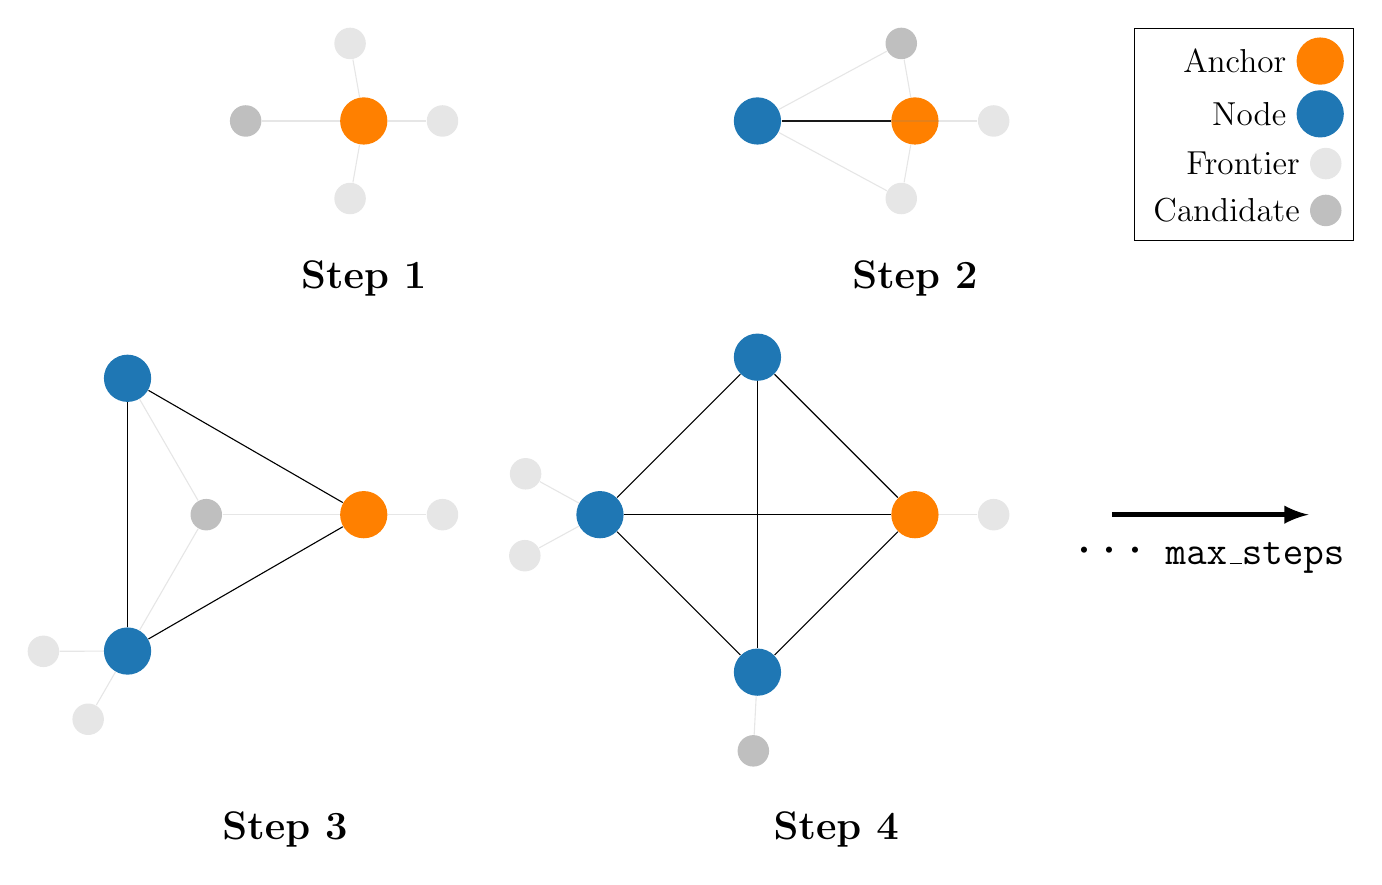
\begin{tikzpicture}[
  scale=1,   
  anchornode/.style={fill=orange, minimum size=6mm, circle},
  frontiernode/.style={fill=gray, minimum size=4mm, circle, opacity=0.2},
  nodenode/.style={fill={rgb,255:red,31;green,119;blue,180}, minimum size=6mm, circle},
  candidatenode/.style={fill=gray, minimum size=4mm, circle, opacity=0.5}
]
  % \Large \textbf{Step} 1
  \begin{scope}[shift={(2,0)}]
    \draw
      (0.0:0) node[anchornode] (0){}
      (0.0:1) node[frontiernode] (-1){}
      (0.0:-1.5) node[candidatenode] (-2){}
      (100:1) node[frontiernode] (-3){}
      (260:1) node[frontiernode] (-4){};
    \begin{scope}[-]
      \draw[draw=gray, thin, opacity=0.2] (0) to (-1);
      \draw[draw=gray, thin, opacity=0.2] (0) to (-2);
      \draw[draw=gray, thin, opacity=0.2] (0) to (-3);
      \draw[draw=gray, thin, opacity=0.2] (0) to (-4);
    \end{scope}
    \node at (0,-2) {\Large \textbf{Step 1}};
  \end{scope}

  % \Large \textbf{Step} 2
  \begin{scope}[shift={(9,0)}]
    \draw
      (0.0:0) node[anchornode] (0){}
      (0.0:1) node[frontiernode] (-1){}
      (180.0:2) node[nodenode] (1){}
      (100:1) node[candidatenode] (-3){}
      (260:1) node[frontiernode] (-4){};
    \begin{scope}[-]
      \draw (0) to (1);
      \draw[draw=gray, thin, opacity=0.2] (0) to (-3);
      \draw[draw=gray, thin, opacity=0.2] (1) to (-1);
      \draw[draw=gray, thin, opacity=0.2] (-3) to (1);
      \draw[draw=gray, thin, opacity=0.2] (0) to (-4);
      \draw[draw=gray, thin, opacity=0.2] (1) to (-4);
    \end{scope}
    \node at (0,-2) {\Large \textbf{Step 2}};
  \end{scope}

  % \Large \textbf{Step} 3
  \begin{scope}[shift={(0,-5)}]
    \draw
      (0.0:0) node[fill=gray, minimum size=4mm, circle, opacity=0.5] (-6){}
      (0.0:3) node[frontiernode] (-1){}
      (0.0:2) node[anchornode] (0){}
      (120.0:2) node[nodenode] (1){}
      (240.0:3) node[frontiernode] (-4){}
      (220.0:2.7) node[frontiernode] (-5){}
      (240.0:2) node[nodenode] (2){};
    \begin{scope}[-]
      \draw[draw=gray, thin, opacity=0.2] (0) to (-1);
      \draw (0) to (1);
      \draw (0) to (2);
      \draw (1) to (2);
      \draw[draw=gray, thin, opacity=0.2] (2) to (-4);
      \draw[draw=gray, thin, opacity=0.2] (2) to (-5);
      \draw[draw=gray, thin, opacity=0.2] (1) to (-6);
      \draw[draw=gray, thin, opacity=0.2] (2) to (-6);
      \draw[draw=gray, thin, opacity=0.2] (0) to (-6);
    \end{scope}
    \node at (1,-4) {\Large \textbf{Step 3}};
  \end{scope}

  % \Large \textbf{Step} 4
  \begin{scope}[shift={(7,-5)}]
    \draw
      (0.0:3) node[frontiernode] (-1){}
      (0.0:2) node[anchornode] (0){}
      (90.0:2) node[nodenode] (1){}
      (180.0:2) node[nodenode] (2){}
      (270.0:2) node[nodenode] (3){}
      (269.0:3) node[candidatenode] (-6){}
      (190.0:3) node[frontiernode] (-4){}
      (170.0:2.99) node[frontiernode] (-5){};
    \begin{scope}[-]
      \draw[draw=gray, thin, opacity=0.2] (0) to (-1);
      \draw (0) to (1);
      \draw (0) to (2);
      \draw (0) to (3);
      \draw (1) to (2);
      \draw (1) to (3);
      \draw (2) to (3);
      \draw[draw=gray, thin, opacity=0.2] (2) to (-4);
      \draw[draw=gray, thin, opacity=0.2] (2) to (-5);
      \draw[draw=gray, thin, opacity=0.2] (3) to (-6);
    \end{scope}
    \node at (1,-4) {\Large \textbf{Step 4}};
  \end{scope}

  % Dots
  \begin{scope}[shift={(11,-8)}]
    \draw[->, >=latex, line width=2pt] (0.5,3) --  node[label= below:\Large\textbf{\huge $\cdots$} \texttt{max\_steps}] {} (3,3);
  \end{scope}

  \matrix [draw, below left, row sep=2pt] at (current bounding box.north east) {
    \node [anchornode, label=left:{\large Anchor}] {}; \\ 
    \node [nodenode, label=left:{\large Node}] {}; \\
    \node [frontiernode, label=left:{\large Frontier}] {}; \\
    \node [candidatenode, label=left:{\large Candidate}] {}; \\
  };
\end{tikzpicture}
}
            \subcaption{Anomaly structure search}
            \label{fig:anomaly_growth}
        \end{minipage}};
        
        % Arrows
        \draw[->] (fig1) -- (fig2) node[midway, above] {\scriptsize Extract};
        \draw[->] (fig2) -- (fig3) node[midway, right] {\scriptsize Search};
        \draw[implies-implies,double equal sign distance, line width=1pt] (fig4) -- (fig3) node[midway, below] {};
    \end{tikzpicture}
    }
    \caption{\footnotesize OES construction and anomalous structure search procedures}
    \label{fig:decoder_process}
\end{figure}
\vspace*{-30pt}
% \vspace*{-30pt}
\begin{algorithm}[H]
\caption{Greedy Search for Anomalous Structures}
\label{algo:algo}
\scriptsize
\begin{algorithmic}[1]
\REQUIRE Graph $G$, starting node $u$, threshold $T_F$, \texttt{max\_steps}, \texttt{max\_no\_change}
\ENSURE Anomalous structure $G'$, Anomaly score \texttt{score}

\STATE Initialize $G' \leftarrow \{u\}$, \texttt{steps} $\leftarrow 0$, \texttt{no\_change\_steps} $\leftarrow 0$, \texttt{score} $\leftarrow 0$

\WHILE{\texttt{steps} $<$ \texttt{max\_steps}}
    \STATE \texttt{steps} $\leftarrow$ \texttt{steps} + 1
    \STATE Initialize $best\_freq \leftarrow \infty$, $G'' \leftarrow G'$
    \STATE Sample a subset of \texttt{max\_cands} candidate nodes from the neighborhood frontier of $G'$
    \FOR{each sampled node $v$}
        \STATE $G_{\text{temp}} \leftarrow G' \cup \{v\}$
        \IF{$Freq_G(G_{\text{temp}}) < best\_freq$}
            \STATE $best\_freq \leftarrow Freq_G(G_{\text{temp}})$
            \STATE $G'' \leftarrow G_{\text{temp}}$
        \ENDIF
    \ENDFOR
    \STATE $G' \leftarrow G''$
    \IF{$Freq_G(G') < T_F$} 
        \STATE Mark $G'$ and all its nodes as anomalies
        \STATE \textbf{break} 
    \ENDIF
    \STATE \texttt{no\_change\_steps} $\leftarrow$ \texttt{no\_change\_steps} + 1 if $Freq_G(G')$ unchanged else 0
    \IF{\texttt{no\_change\_steps} $\geq$ \texttt{max\_no\_change}} 
        \STATE \textbf{break} 
    \ENDIF
\ENDWHILE
\STATE \texttt{score} $\leftarrow 1 - Freq_G(G')$
\RETURN $G', \texttt{score}$
\end{algorithmic}
\end{algorithm}

\vspace*{-30pt}

\subsubsection{Algorithm}
The method adopts a greedy search (Algorithm \ref{algo:algo}) for anomalous structures $G'$, beginning from a starting node $u$ and growing by iteratively selecting a candidate node $u'$ from the current neighborhood frontier to obtain the most infrequent structure at each step. This process continues until one of the following conditions is met: $Freq_G(G') < T_F$, the maximum subgraph order (\texttt{max\_steps}) is reached, or no significant change is observed (\texttt{max\_no\_change}). If the first condition is satisfied, the final small structure and all its nodes are identified as anomalies based on the final frequency, with the anomaly score defined as $1 - Freq_G(G')$.

This can be viewed as a monotonic walk in the search space of OES due to the preserved anti-monotonicity property. If the resulting neighborhood $G'$ of $u$ is grown by the ordered sequence of subgraphs $G^{(1)}_u \subseteq G^{(2)}_u \subseteq \dots \subseteq G^{(l)}_u$ such that $l \in \llbracket 1, \texttt{max\_steps} \rrbracket$ and $G' = G^{(l)}_u$, a monotonic path of embedding search $\phi(G^{(1)}_u) \preceq \phi(G^{(2)}_u) \preceq \dots \preceq \phi(G^{(l)}_u)$ is observed, because $Freq_G$ is anti-monotonic: \[Freq_G(G^{(l)}_u) \le \dots \le Freq_G(G^{(2)}_u) \le Freq_G(G^{(1)}_u)\]

\section{Experimental Evaluation}
\label{sec:eval}
% \subsection{Experimental Settings and Datasets}
To evaluate Minomaly, we use the datasets listed in Table \ref{tab:datasets}, which are provided by \cite{NEURIPS2022-acc1ec4a,JMLR:v25:23-0963} and adopted in \cite{chen2020generative,ding2019deep,fan2020anomalydae,gu2024three,yuan2024higherorder}. %We follow the evaluation protocol described in \cite{ding2019deep}. %These synthetic outliers are combined with real datasets. We rely on these injections due to the scarcity of datasets that explicitly distinguish between structural and contextual outliers.

\begin{wraptable}[7]{r}{6.2cm}
\centering
\vspace*{-20pt}
\caption{Statistics of datasets}
\label{tab:datasets}
\scriptsize
\begin{tabular}{lccccccc}
\toprule
Dataset       & Nodes  & Edges   & Avg. Degree & Anomalies \\
\midrule
Cora     & 2,708  & 11,060  & 4.1         & 70 (5.1\%)    \\
Amazon   & 13,752 & 515,042 & 37.2        & 350 (5.0\%)    \\
Flickr   & 89,250 & 933,804 & 10.5        & 2,240 (4.9\%)    \\
\bottomrule
\end{tabular}
\end{wraptable}

We conducted our experiments following the protocol in \cite{NEURIPS2022-acc1ec4a}, using a Linux machine with Python 3.12.2, CUDA 12, and an NVIDIA RTX A2000 GPU (12 GB). Minomaly was implemented using PyTorch 2.4, Torch Geometric 2.6, and DeepSNAP, while the benchmarked methods were implemented using \cite{JMLR:v25:23-0963}.

The Minomaly's OES, pretrained on synthetic graphs, achieves \(95\%\) accuracy in determining whether one graph is a subgraph of another with linear time complexity \cite{ying2024representation}. It was also used for processing all the benchmarked datasets.% GUIDE \cite{yuan2024higherorder}, which shares Minomaly's core approach of counting, uses a CPU-intensive graph motif counting algorithm for structural features but is excluded from the benchmark due to memory limitations.

We compared Minomaly to existing deep learning GAD methods: GCNAE \cite{kipf2016variational,NEURIPS2022-acc1ec4a}, DOMINANT, DONE, AdONE, AnomalyDAE, and CONAD across binary classification metrics, including area under ROC (AUC), Average Precision (AP), Recall, and Precision.

Minomaly’s hyperparameters, presented in Table \ref{tab:minomaly_hyperparameters}, are interpretable and manually tuned to improve results. This allows refinement after each run by filtering user-relative positives, expanding search spaces, or reducing computational resources, without random hyperparameter search. We set the hyperparameters shown in Table \ref{tab:minomaly_hyperparameters} for each dataset, fixing the OES dimension to $d = 64$, \texttt{min\_neigh\_size} to $1$, and \texttt{max\_neigh\_size} to $30$. Additionally, we used $8$ threads for the search phase. The results corresponding to each hyperparameter configuration (C\textsubscript{1}, A\textsubscript{1}, F\textsubscript{1}, F\textsubscript{2}, F\textsubscript{3}) are detailed in Table \ref{tab:minomaly_results}.

\vspace*{-30pt}
% \begin{table}[H]
% \centering
% \caption{Minomaly hyperparameters}
% \label{tab:minomaly_hyperparameters}
% \scriptsize
% \begin{tabular}{|c|l|r|r|r|c|r|r|r|r|r|r|}
% \hline
% \textbf{Run} & \textbf{Dataset} & \boldmath$RG$ \textbf{size} & \boldmath$T_F$ & \texttt{max\_steps} & \texttt{max\_no\_change} & \texttt{max\_cands} & \texttt{batch\_size} \\ \hline
% C\textsubscript{1}   & Cora   & 10,000  & $\frac{35}{2708}=0.013$    & 7  & 5  & All & 1000 \\ \hline
% A\textsubscript{1}   & Amazon & 50,000   & $\frac{150}{13752}=0.011$  & 11 & 3  & 20 & 10,000 \\ \hline
% F\textsubscript{1}   & Flickr & 150,000  & $\frac{1000}{89250}=0.011$ & 7  & 3  & 10 & 10,000 \\ \hline
% F\textsubscript{2}   & Flickr & 200,000  & $\frac{1000}{89250}=0.011$ & 7  & 3  & 10 & 12,500 \\ \hline
% F\textsubscript{3}   & Flickr & 250,000  & $\frac{1000}{89250}=0.011$ & 7  & 3  & 10 & 12,500 \\ \hline
% \end{tabular}
% \end{table}
% \vspace*{-30pt}
% \subsection{Overall Results}
\vspace*{-30pt}
\paragraph{Impact of using starting nodes}
As shown in Table~\ref{tab:minomaly_results}, at least 70\% of the starting nodes extracted by methods (a) and (b) desctribed in ~\ref{sec:anomaly_search}, are true positives. By employing these methods, Using these methods, we process at most 50\% of the nodes in Cora and Amazon and 30\% in Flickr, the largest dataset. This approach achieves high recall by including all nodes in anomalous neighborhoods and high precision by avoiding unnecessary searches in areas prone to false positives, thus reducing computation time and improving performance.  
\paragraph{Dataset characteristics and hyperparameters}
Amazon and Flickr have high node degrees, particularly Amazon, yet selecting \texttt{max\_cands} of 20 and 10 nodes, respectively, from the frontier was sufficient for strong results. However, high node degrees also contributed to longer search times for Amazon. Additionally, increasing the size of $RG$ of Flickr (F\textsubscript{1}, F\textsubscript{2}, F\textsubscript{3}) improves detection quality  but increases embedding time.

% \vspace*{-30pt}
% \begin{table}[H]
% \centering
% \caption{Minomaly Results}
% \label{tab:minomaly_results}
% \scriptsize
% \begin{tabular}{|c|c|c|r|r|r|r|r|r|r|}
% \hline
% \textbf{Run} & \textbf{Starting nodes} & \textbf{Positive nodes} & \textbf{AUC} & \textbf{AP} & \textbf{Recall} & \textbf{Precision} & \textbf{Search} & \textbf{OES build} \\ \hline
% C\textsubscript{1}   & $\frac{1120}{2708}=41.4\%$  & $\frac{67}{70}=95.7\%$  & 95.25\%  & 74.62\%  & 91.43\%  & 83.12\%  & 293 s   & 22 s \\ \hline
% A\textsubscript{1}   & $\frac{6977}{13752}=50.7\%$ & $\frac{300}{350}=85.7\%$ & 95.40\%  & 57.66\%  & 92.86\%  & 55.65\%  & 2770 s  & 118 s \\ \hline
% F\textsubscript{1}   & $\frac{15988}{89250}=17.9\%$ & $\frac{1535}{2240}=68.5\%$ & 90.52\%  & 77.73\%  & 81.21\%  & 94.34\%  & 2521 s  & 542 s \\ \hline
% F\textsubscript{2}   & $\frac{20057}{89250}=22.5\%$ & $\frac{1736}{2240}=77.5\%$ & 93.56\%  & 85.28\%  & 87.19\%  & 94.99\%  & 4098 s  & 1021 s \\ \hline
% F\textsubscript{3}   & $\frac{24074}{89250}=27.0\%$ & $\frac{1898}{2240}=84.7\%$ & 94.06\%  & 85.82\%  & 88.21\%  & 93.73\%  & 5690 s  & 1335 s \\ \hline
% \end{tabular}
% \end{table}

\vspace*{-30pt}
\paragraph{Performance and interpretation}
Minomaly achieved high scores across all datasets and metrics (see Table~\ref{tab:minomaly_results}) and successfully interpreted all mined anomalous patterns (see Figure~\ref{fig:interpret_results}). By interpreting the false positives on Amazon, we justify the low precision by the presence of patterns labeled as normal that are similar to the true positive patterns.

% \vspace*{-30pt}
\begin{figure}[H]
    \centering
    \begin{subfigure}{0.2\textwidth}
        \resizebox{\linewidth}{!}{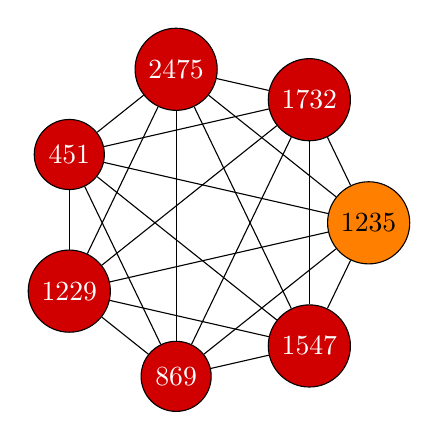
\begin{tikzpicture}
  \draw
    (0.0:2) node[fill=orange, minimum size=4mm, circle, draw] (1235){1235}
    (51.429:2) node[fill={rgb,140:red,255;green,0;blue,0}, minimum size=2mm, circle, draw, text=white] (1732){1732}
    (102.857:2) node[fill={rgb,140:red,255;green,0;blue,0}, minimum size=2mm, circle, draw, text=white] (2475){2475}
    (154.286:2) node[fill={rgb,140:red,255;green,0;blue,0}, minimum size=2mm, circle, draw, text=white] (451){451}
    (205.714:2) node[fill={rgb,140:red,255;green,0;blue,0}, minimum size=2mm, circle, draw, text=white] (1229){1229}
    (257.143:2) node[fill={rgb,140:red,255;green,0;blue,0}, minimum size=2mm, circle, draw, text=white] (869){869}
    (308.571:2) node[fill={rgb,140:red,255;green,0;blue,0}, minimum size=2mm, circle, draw, text=white] (1547){1547};
  \begin{scope}[-]
    \draw (1235) to (1732);
    \draw (1235) to (2475);
    \draw (1235) to (451);
    \draw (1235) to (1229);
    \draw (1235) to (869);
    \draw (1235) to (1547);
    \draw (1732) to (2475);
    \draw (1732) to (451);
    \draw (1732) to (1229);
    \draw (1732) to (869);
    \draw (1732) to (1547);
    \draw (2475) to (451);
    \draw (2475) to (1229);
    \draw (2475) to (869);
    \draw (2475) to (1547);
    \draw (451) to (1229);
    \draw (451) to (869);
    \draw (451) to (1547);
    \draw (1229) to (869);
    \draw (1229) to (1547);
    \draw (869) to (1547);
  \end{scope}
\end{tikzpicture}}
        \caption{True positive}
        \label{fig:true_positive}
    \end{subfigure}
    \hfill
    % \begin{subfigure}{0.3\textwidth}
    %     \resizebox{\linewidth}{!}{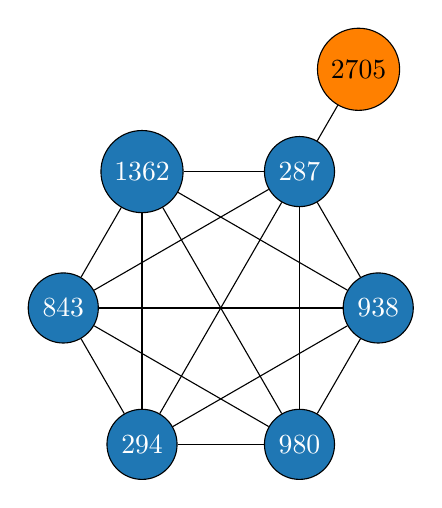
\begin{tikzpicture}
  \draw
    (60.0:2) node[fill={rgb,255:red,31;green,119;blue,180}, minimum size=2mm, circle, draw, text=white] (287){287}
    (0.0:2) node[fill={rgb,255:red,31;green,119;blue,180}, minimum size=2mm, circle, draw, text=white] (938){938}
    (120.0:2) node[fill={rgb,255:red,31;green,119;blue,180}, minimum size=2mm, circle, draw, text=white] (1362){1362}
    (180.0:2) node[fill={rgb,255:red,31;green,119;blue,180}, minimum size=2mm, circle, draw, text=white] (151){843}
    (240.0:2) node[fill={rgb,255:red,31;green,119;blue,180}, minimum size=2mm, circle, draw, text=white] (2198){294}
    (300.0:2) node[fill={rgb,255:red,31;green,119;blue,180}, minimum size=2mm, circle, draw, text=white] (980){980}
    (60.0:3.5) node[fill=orange, minimum size=4mm, circle, draw] (2705){2705};
  \begin{scope}[-]
    \draw (287) to (938);
    \draw (287) to (2705);
    \draw (287) to (1362);
    \draw (287) to (151);
    \draw (287) to (2198);
    \draw (287) to (980);
    \draw (938) to (1362);
    \draw (938) to (151);
    \draw (938) to (2198);
    \draw (938) to (980);
    \draw (1362) to (151);
    \draw (1362) to (2198);
    \draw (1362) to (980);
    \draw (151) to (2198);
    \draw (151) to (980);
    \draw (2198) to (980);
  \end{scope}
\end{tikzpicture}}
    %     \caption{False positive}
    % \end{subfigure}
    \begin{subfigure}{0.3\textwidth}
        \resizebox{\linewidth}{!}{% This file was created with tikzplotlib v0.9.12.
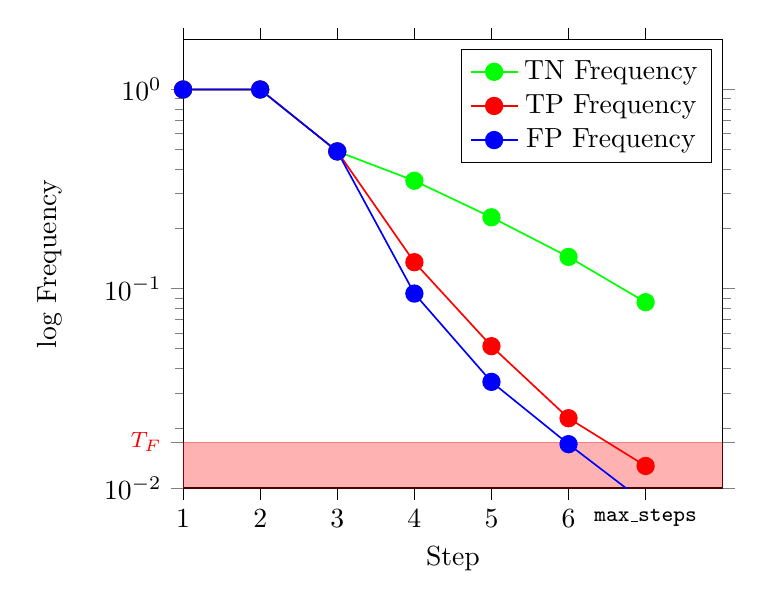
\begin{tikzpicture}

\definecolor{color0}{rgb}{0.12156862745098,0.466666666666667,0.705882352941177}

\begin{axis}[
log basis y={10},
tick align=outside,
tick pos=both,
x grid style={white!69.0196078431373!black},
xlabel={Step},
xmin=1, xmax=8,
xtick style={color=black},
xtick={1,2,3,4,5,6,7},
xticklabels={1,2,3,4,5,6,\footnotesize
\texttt{max\_steps}},
y grid style={white!69.0196078431373!black},
ylabel={$\log$ Frequency},
ymin=0.01, ymax=1.77827941003892,
ymode=log,
extra y ticks={0.017}, % Adding the specific y tick
extra y tick labels={\footnotesize $T_F$}, % Labeling it as T_F
extra y tick style={font=\footnotesize, yticklabel style={color=red}}
]
\path [draw=red, fill=red, opacity=0.3]
(axis cs:1,0.017)
--(axis cs:1,1e-05)
--(axis cs:2,1e-05)
--(axis cs:3,1e-05)
--(axis cs:4,1e-05)
--(axis cs:5,1e-05)
--(axis cs:6,1e-05)
--(axis cs:7,1e-05)
--(axis cs:8,1e-05)
--(axis cs:8,0.017)
--(axis cs:8,0.017)
--(axis cs:7,0.017)
--(axis cs:6,0.017)
--(axis cs:5,0.017)
--(axis cs:4,0.017)
--(axis cs:3,0.017)
--(axis cs:2,0.017)
--(axis cs:1,0.017)
--cycle;

\addplot [semithick, green, mark=*, mark size=3, mark options={solid}]
table {%
1 1
2 1
3 0.489
4 0.3484
5 0.2284
6 0.1444
7 0.0856
};
\addlegendentry{TN Frequency}

\addplot [semithick, red, mark=*, mark size=3, mark options={solid}]
table {%
1 1
2 1
3 0.489
4 0.1359
5 0.0515
6 0.0224
7 0.0129
};
\addlegendentry{TP Frequency}

\addplot [semithick, blue, mark=*, mark size=3, mark options={solid}]
table {%
1 1
2 1.0
3 0.489
4 0.0946
5 0.0341
6 0.0166
7 0.0084
};
\addlegendentry{FP Frequency}
\end{axis}


\end{tikzpicture}
}
        \caption{Frequency changes}
        \label{fig:frequency_track}
    \end{subfigure}
    \hfill
    \begin{subfigure}{0.2\textwidth}
        \resizebox{\linewidth}{!}{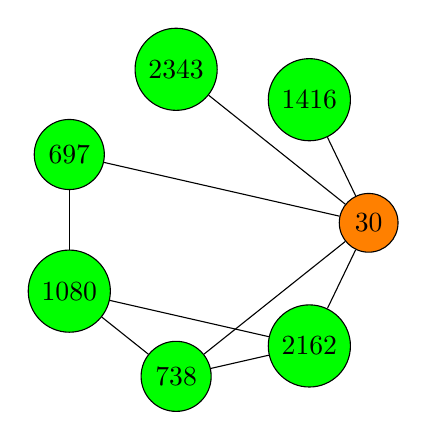
\begin{tikzpicture}
  \draw
    (0.0:2) node[fill=orange, minimum size=4mm, circle, draw] (30){30}
    (51.429:2) node[fill=green, minimum size=2mm, circle, draw] (1416){1416}
    (102.857:2) node[fill=green, minimum size=2mm, circle, draw] (2343){2343}
    (154.286:2) node[fill=green, minimum size=2mm, circle, draw] (697){697}
    (205.714:2) node[fill=green, minimum size=2mm, circle, draw] (1080){1080}
    (257.143:2) node[fill=green, minimum size=2mm, circle, draw] (738){738}
    (308.571:2) node[fill=green, minimum size=2mm, circle, draw] (2162){2162};
  \begin{scope}[-]
    \draw (30) to (1416);
    \draw (30) to (2343);
    \draw (30) to (697);
    \draw (30) to (2162);
    \draw (30) to (738);
    \draw (697) to (1080);
    \draw (1080) to (738);
    \draw (1080) to (2162);
    \draw (738) to (2162);
  \end{scope}
\end{tikzpicture}}
        \caption{True negative}
        \label{fig:false_positive}
    \end{subfigure}
    \caption{\small Minomaly results on the Amazon dataset. It illustrates two examples: an anomalous structure (red) and a normal one (green), along with their frequency change curves.}
    \label{fig:interpret_results}
\end{figure}

\vspace*{-20pt}
\paragraph{Comparison to other methods}
From Fig.~\ref{fig:pr_curve}, we observe low Precision@k %at low recalls 
across all methods, corresponding to low-frequency detected anomalies for Minomaly. This is attributed to the existence of some unlabeled structures that are rarer than the labeled ones, as shown by interpretations. DONE achieves high Precision@k on Cora due to its restrictive anomaly definition but fails to maintain precision on other datasets, unlike our frequency-based method. Overall, Minomaly outperforms reconstruction-loss methods, which fail to capture anomalous patterns across different contexts, as mentioned in Section~\ref{sec:relatedworks}. It achieves this across all metrics and scales efficiently, avoiding memory issues on large datasets like Flickr (see Table \ref{tab:bench_results}).

% Minomaly outperforms other methods in terms of AUC, F1, and AP scores (see Table~\ref{tab:bench_results} and Figure \ref{fig:pr_curve}). This shows that using frequency as a measure of abnormality has proven to be more effective in identifying true anomalies, surpassing reconstruction-loss methods in handling rare patterns. One can also see that Minomaly is scalable, as it avoids out-of-memory errors on large datasets like Flickr (see Table~\ref{tab:bench_results}).

\vspace*{-17pt}
\begin{figure}[H]
    \centering
    \begin{subfigure}{0.32\textwidth}
        \resizebox{\linewidth}{!}{%% Creator: Matplotlib, PGF backend
%%
%% To include the figure in your LaTeX document, write
%%   \input{<filename>.pgf}
%%
%% Make sure the required packages are loaded in your preamble
%%   \usepackage{pgf}
%%
%% Figures using additional raster images can only be included by \input if
%% they are in the same directory as the main LaTeX file. For loading figures
%% from other directories you can use the `import` package
%%   \usepackage{import}
%% and then include the figures with
%%   \import{<path to file>}{<filename>.pgf}
%%
%% Matplotlib used the following preamble
%%
\begingroup%
\makeatletter%
\begin{pgfpicture}%
\pgfpathrectangle{\pgfpointorigin}{\pgfqpoint{5.352315in}{5.178302in}}%
\pgfusepath{use as bounding box, clip}%
\begin{pgfscope}%
\pgfsetbuttcap%
\pgfsetmiterjoin%
\definecolor{currentfill}{rgb}{1.000000,1.000000,1.000000}%
\pgfsetfillcolor{currentfill}%
\pgfsetlinewidth{0.000000pt}%
\definecolor{currentstroke}{rgb}{1.000000,1.000000,1.000000}%
\pgfsetstrokecolor{currentstroke}%
\pgfsetdash{}{0pt}%
\pgfpathmoveto{\pgfqpoint{-0.000000in}{0.000000in}}%
\pgfpathlineto{\pgfqpoint{5.352315in}{0.000000in}}%
\pgfpathlineto{\pgfqpoint{5.352315in}{5.178302in}}%
\pgfpathlineto{\pgfqpoint{-0.000000in}{5.178302in}}%
\pgfpathclose%
\pgfusepath{fill}%
\end{pgfscope}%
\begin{pgfscope}%
\pgfsetbuttcap%
\pgfsetmiterjoin%
\definecolor{currentfill}{rgb}{1.000000,1.000000,1.000000}%
\pgfsetfillcolor{currentfill}%
\pgfsetlinewidth{0.000000pt}%
\definecolor{currentstroke}{rgb}{0.000000,0.000000,0.000000}%
\pgfsetstrokecolor{currentstroke}%
\pgfsetstrokeopacity{0.000000}%
\pgfsetdash{}{0pt}%
\pgfpathmoveto{\pgfqpoint{0.553704in}{0.499691in}}%
\pgfpathlineto{\pgfqpoint{5.203704in}{0.499691in}}%
\pgfpathlineto{\pgfqpoint{5.203704in}{5.029691in}}%
\pgfpathlineto{\pgfqpoint{0.553704in}{5.029691in}}%
\pgfpathclose%
\pgfusepath{fill}%
\end{pgfscope}%
\begin{pgfscope}%
\pgfpathrectangle{\pgfqpoint{0.553704in}{0.499691in}}{\pgfqpoint{4.650000in}{4.530000in}} %
\pgfusepath{clip}%
\pgfsetrectcap%
\pgfsetroundjoin%
\pgfsetlinewidth{0.803000pt}%
\definecolor{currentstroke}{rgb}{0.690196,0.690196,0.690196}%
\pgfsetstrokecolor{currentstroke}%
\pgfsetdash{}{0pt}%
\pgfpathmoveto{\pgfqpoint{0.765068in}{0.499691in}}%
\pgfpathlineto{\pgfqpoint{0.765068in}{5.029691in}}%
\pgfusepath{stroke}%
\end{pgfscope}%
\begin{pgfscope}%
\pgfsetbuttcap%
\pgfsetroundjoin%
\definecolor{currentfill}{rgb}{0.000000,0.000000,0.000000}%
\pgfsetfillcolor{currentfill}%
\pgfsetlinewidth{0.803000pt}%
\definecolor{currentstroke}{rgb}{0.000000,0.000000,0.000000}%
\pgfsetstrokecolor{currentstroke}%
\pgfsetdash{}{0pt}%
\pgfsys@defobject{currentmarker}{\pgfqpoint{0.000000in}{-0.048611in}}{\pgfqpoint{0.000000in}{0.000000in}}{%
\pgfpathmoveto{\pgfqpoint{0.000000in}{0.000000in}}%
\pgfpathlineto{\pgfqpoint{0.000000in}{-0.048611in}}%
\pgfusepath{stroke,fill}%
}%
\begin{pgfscope}%
\pgfsys@transformshift{0.765068in}{0.499691in}%
\pgfsys@useobject{currentmarker}{}%
\end{pgfscope}%
\end{pgfscope}%
\begin{pgfscope}%
\pgftext[x=0.765068in,y=0.402469in,,top]{\rmfamily\fontsize{10.000000}{12.000000}\selectfont \(\displaystyle 0.0\)}%
\end{pgfscope}%
\begin{pgfscope}%
\pgfpathrectangle{\pgfqpoint{0.553704in}{0.499691in}}{\pgfqpoint{4.650000in}{4.530000in}} %
\pgfusepath{clip}%
\pgfsetrectcap%
\pgfsetroundjoin%
\pgfsetlinewidth{0.803000pt}%
\definecolor{currentstroke}{rgb}{0.690196,0.690196,0.690196}%
\pgfsetstrokecolor{currentstroke}%
\pgfsetdash{}{0pt}%
\pgfpathmoveto{\pgfqpoint{1.610522in}{0.499691in}}%
\pgfpathlineto{\pgfqpoint{1.610522in}{5.029691in}}%
\pgfusepath{stroke}%
\end{pgfscope}%
\begin{pgfscope}%
\pgfsetbuttcap%
\pgfsetroundjoin%
\definecolor{currentfill}{rgb}{0.000000,0.000000,0.000000}%
\pgfsetfillcolor{currentfill}%
\pgfsetlinewidth{0.803000pt}%
\definecolor{currentstroke}{rgb}{0.000000,0.000000,0.000000}%
\pgfsetstrokecolor{currentstroke}%
\pgfsetdash{}{0pt}%
\pgfsys@defobject{currentmarker}{\pgfqpoint{0.000000in}{-0.048611in}}{\pgfqpoint{0.000000in}{0.000000in}}{%
\pgfpathmoveto{\pgfqpoint{0.000000in}{0.000000in}}%
\pgfpathlineto{\pgfqpoint{0.000000in}{-0.048611in}}%
\pgfusepath{stroke,fill}%
}%
\begin{pgfscope}%
\pgfsys@transformshift{1.610522in}{0.499691in}%
\pgfsys@useobject{currentmarker}{}%
\end{pgfscope}%
\end{pgfscope}%
\begin{pgfscope}%
\pgftext[x=1.610522in,y=0.402469in,,top]{\rmfamily\fontsize{10.000000}{12.000000}\selectfont \(\displaystyle 0.2\)}%
\end{pgfscope}%
\begin{pgfscope}%
\pgfpathrectangle{\pgfqpoint{0.553704in}{0.499691in}}{\pgfqpoint{4.650000in}{4.530000in}} %
\pgfusepath{clip}%
\pgfsetrectcap%
\pgfsetroundjoin%
\pgfsetlinewidth{0.803000pt}%
\definecolor{currentstroke}{rgb}{0.690196,0.690196,0.690196}%
\pgfsetstrokecolor{currentstroke}%
\pgfsetdash{}{0pt}%
\pgfpathmoveto{\pgfqpoint{2.455977in}{0.499691in}}%
\pgfpathlineto{\pgfqpoint{2.455977in}{5.029691in}}%
\pgfusepath{stroke}%
\end{pgfscope}%
\begin{pgfscope}%
\pgfsetbuttcap%
\pgfsetroundjoin%
\definecolor{currentfill}{rgb}{0.000000,0.000000,0.000000}%
\pgfsetfillcolor{currentfill}%
\pgfsetlinewidth{0.803000pt}%
\definecolor{currentstroke}{rgb}{0.000000,0.000000,0.000000}%
\pgfsetstrokecolor{currentstroke}%
\pgfsetdash{}{0pt}%
\pgfsys@defobject{currentmarker}{\pgfqpoint{0.000000in}{-0.048611in}}{\pgfqpoint{0.000000in}{0.000000in}}{%
\pgfpathmoveto{\pgfqpoint{0.000000in}{0.000000in}}%
\pgfpathlineto{\pgfqpoint{0.000000in}{-0.048611in}}%
\pgfusepath{stroke,fill}%
}%
\begin{pgfscope}%
\pgfsys@transformshift{2.455977in}{0.499691in}%
\pgfsys@useobject{currentmarker}{}%
\end{pgfscope}%
\end{pgfscope}%
\begin{pgfscope}%
\pgftext[x=2.455977in,y=0.402469in,,top]{\rmfamily\fontsize{10.000000}{12.000000}\selectfont \(\displaystyle 0.4\)}%
\end{pgfscope}%
\begin{pgfscope}%
\pgfpathrectangle{\pgfqpoint{0.553704in}{0.499691in}}{\pgfqpoint{4.650000in}{4.530000in}} %
\pgfusepath{clip}%
\pgfsetrectcap%
\pgfsetroundjoin%
\pgfsetlinewidth{0.803000pt}%
\definecolor{currentstroke}{rgb}{0.690196,0.690196,0.690196}%
\pgfsetstrokecolor{currentstroke}%
\pgfsetdash{}{0pt}%
\pgfpathmoveto{\pgfqpoint{3.301431in}{0.499691in}}%
\pgfpathlineto{\pgfqpoint{3.301431in}{5.029691in}}%
\pgfusepath{stroke}%
\end{pgfscope}%
\begin{pgfscope}%
\pgfsetbuttcap%
\pgfsetroundjoin%
\definecolor{currentfill}{rgb}{0.000000,0.000000,0.000000}%
\pgfsetfillcolor{currentfill}%
\pgfsetlinewidth{0.803000pt}%
\definecolor{currentstroke}{rgb}{0.000000,0.000000,0.000000}%
\pgfsetstrokecolor{currentstroke}%
\pgfsetdash{}{0pt}%
\pgfsys@defobject{currentmarker}{\pgfqpoint{0.000000in}{-0.048611in}}{\pgfqpoint{0.000000in}{0.000000in}}{%
\pgfpathmoveto{\pgfqpoint{0.000000in}{0.000000in}}%
\pgfpathlineto{\pgfqpoint{0.000000in}{-0.048611in}}%
\pgfusepath{stroke,fill}%
}%
\begin{pgfscope}%
\pgfsys@transformshift{3.301431in}{0.499691in}%
\pgfsys@useobject{currentmarker}{}%
\end{pgfscope}%
\end{pgfscope}%
\begin{pgfscope}%
\pgftext[x=3.301431in,y=0.402469in,,top]{\rmfamily\fontsize{10.000000}{12.000000}\selectfont \(\displaystyle 0.6\)}%
\end{pgfscope}%
\begin{pgfscope}%
\pgfpathrectangle{\pgfqpoint{0.553704in}{0.499691in}}{\pgfqpoint{4.650000in}{4.530000in}} %
\pgfusepath{clip}%
\pgfsetrectcap%
\pgfsetroundjoin%
\pgfsetlinewidth{0.803000pt}%
\definecolor{currentstroke}{rgb}{0.690196,0.690196,0.690196}%
\pgfsetstrokecolor{currentstroke}%
\pgfsetdash{}{0pt}%
\pgfpathmoveto{\pgfqpoint{4.146886in}{0.499691in}}%
\pgfpathlineto{\pgfqpoint{4.146886in}{5.029691in}}%
\pgfusepath{stroke}%
\end{pgfscope}%
\begin{pgfscope}%
\pgfsetbuttcap%
\pgfsetroundjoin%
\definecolor{currentfill}{rgb}{0.000000,0.000000,0.000000}%
\pgfsetfillcolor{currentfill}%
\pgfsetlinewidth{0.803000pt}%
\definecolor{currentstroke}{rgb}{0.000000,0.000000,0.000000}%
\pgfsetstrokecolor{currentstroke}%
\pgfsetdash{}{0pt}%
\pgfsys@defobject{currentmarker}{\pgfqpoint{0.000000in}{-0.048611in}}{\pgfqpoint{0.000000in}{0.000000in}}{%
\pgfpathmoveto{\pgfqpoint{0.000000in}{0.000000in}}%
\pgfpathlineto{\pgfqpoint{0.000000in}{-0.048611in}}%
\pgfusepath{stroke,fill}%
}%
\begin{pgfscope}%
\pgfsys@transformshift{4.146886in}{0.499691in}%
\pgfsys@useobject{currentmarker}{}%
\end{pgfscope}%
\end{pgfscope}%
\begin{pgfscope}%
\pgftext[x=4.146886in,y=0.402469in,,top]{\rmfamily\fontsize{10.000000}{12.000000}\selectfont \(\displaystyle 0.8\)}%
\end{pgfscope}%
\begin{pgfscope}%
\pgfpathrectangle{\pgfqpoint{0.553704in}{0.499691in}}{\pgfqpoint{4.650000in}{4.530000in}} %
\pgfusepath{clip}%
\pgfsetrectcap%
\pgfsetroundjoin%
\pgfsetlinewidth{0.803000pt}%
\definecolor{currentstroke}{rgb}{0.690196,0.690196,0.690196}%
\pgfsetstrokecolor{currentstroke}%
\pgfsetdash{}{0pt}%
\pgfpathmoveto{\pgfqpoint{4.992341in}{0.499691in}}%
\pgfpathlineto{\pgfqpoint{4.992341in}{5.029691in}}%
\pgfusepath{stroke}%
\end{pgfscope}%
\begin{pgfscope}%
\pgfsetbuttcap%
\pgfsetroundjoin%
\definecolor{currentfill}{rgb}{0.000000,0.000000,0.000000}%
\pgfsetfillcolor{currentfill}%
\pgfsetlinewidth{0.803000pt}%
\definecolor{currentstroke}{rgb}{0.000000,0.000000,0.000000}%
\pgfsetstrokecolor{currentstroke}%
\pgfsetdash{}{0pt}%
\pgfsys@defobject{currentmarker}{\pgfqpoint{0.000000in}{-0.048611in}}{\pgfqpoint{0.000000in}{0.000000in}}{%
\pgfpathmoveto{\pgfqpoint{0.000000in}{0.000000in}}%
\pgfpathlineto{\pgfqpoint{0.000000in}{-0.048611in}}%
\pgfusepath{stroke,fill}%
}%
\begin{pgfscope}%
\pgfsys@transformshift{4.992341in}{0.499691in}%
\pgfsys@useobject{currentmarker}{}%
\end{pgfscope}%
\end{pgfscope}%
\begin{pgfscope}%
\pgftext[x=4.992341in,y=0.402469in,,top]{\rmfamily\fontsize{10.000000}{12.000000}\selectfont \(\displaystyle 1.0\)}%
\end{pgfscope}%
\begin{pgfscope}%
\pgftext[x=2.878704in,y=0.223457in,,top]{\rmfamily\fontsize{10.000000}{12.000000}\selectfont Recall}%
\end{pgfscope}%
\begin{pgfscope}%
\pgfpathrectangle{\pgfqpoint{0.553704in}{0.499691in}}{\pgfqpoint{4.650000in}{4.530000in}} %
\pgfusepath{clip}%
\pgfsetrectcap%
\pgfsetroundjoin%
\pgfsetlinewidth{0.803000pt}%
\definecolor{currentstroke}{rgb}{0.690196,0.690196,0.690196}%
\pgfsetstrokecolor{currentstroke}%
\pgfsetdash{}{0pt}%
\pgfpathmoveto{\pgfqpoint{0.553704in}{0.705600in}}%
\pgfpathlineto{\pgfqpoint{5.203704in}{0.705600in}}%
\pgfusepath{stroke}%
\end{pgfscope}%
\begin{pgfscope}%
\pgfsetbuttcap%
\pgfsetroundjoin%
\definecolor{currentfill}{rgb}{0.000000,0.000000,0.000000}%
\pgfsetfillcolor{currentfill}%
\pgfsetlinewidth{0.803000pt}%
\definecolor{currentstroke}{rgb}{0.000000,0.000000,0.000000}%
\pgfsetstrokecolor{currentstroke}%
\pgfsetdash{}{0pt}%
\pgfsys@defobject{currentmarker}{\pgfqpoint{-0.048611in}{0.000000in}}{\pgfqpoint{0.000000in}{0.000000in}}{%
\pgfpathmoveto{\pgfqpoint{0.000000in}{0.000000in}}%
\pgfpathlineto{\pgfqpoint{-0.048611in}{0.000000in}}%
\pgfusepath{stroke,fill}%
}%
\begin{pgfscope}%
\pgfsys@transformshift{0.553704in}{0.705600in}%
\pgfsys@useobject{currentmarker}{}%
\end{pgfscope}%
\end{pgfscope}%
\begin{pgfscope}%
\pgftext[x=0.279012in,y=0.657375in,left,base]{\rmfamily\fontsize{10.000000}{12.000000}\selectfont \(\displaystyle 0.0\)}%
\end{pgfscope}%
\begin{pgfscope}%
\pgfpathrectangle{\pgfqpoint{0.553704in}{0.499691in}}{\pgfqpoint{4.650000in}{4.530000in}} %
\pgfusepath{clip}%
\pgfsetrectcap%
\pgfsetroundjoin%
\pgfsetlinewidth{0.803000pt}%
\definecolor{currentstroke}{rgb}{0.690196,0.690196,0.690196}%
\pgfsetstrokecolor{currentstroke}%
\pgfsetdash{}{0pt}%
\pgfpathmoveto{\pgfqpoint{0.553704in}{1.529237in}}%
\pgfpathlineto{\pgfqpoint{5.203704in}{1.529237in}}%
\pgfusepath{stroke}%
\end{pgfscope}%
\begin{pgfscope}%
\pgfsetbuttcap%
\pgfsetroundjoin%
\definecolor{currentfill}{rgb}{0.000000,0.000000,0.000000}%
\pgfsetfillcolor{currentfill}%
\pgfsetlinewidth{0.803000pt}%
\definecolor{currentstroke}{rgb}{0.000000,0.000000,0.000000}%
\pgfsetstrokecolor{currentstroke}%
\pgfsetdash{}{0pt}%
\pgfsys@defobject{currentmarker}{\pgfqpoint{-0.048611in}{0.000000in}}{\pgfqpoint{0.000000in}{0.000000in}}{%
\pgfpathmoveto{\pgfqpoint{0.000000in}{0.000000in}}%
\pgfpathlineto{\pgfqpoint{-0.048611in}{0.000000in}}%
\pgfusepath{stroke,fill}%
}%
\begin{pgfscope}%
\pgfsys@transformshift{0.553704in}{1.529237in}%
\pgfsys@useobject{currentmarker}{}%
\end{pgfscope}%
\end{pgfscope}%
\begin{pgfscope}%
\pgftext[x=0.279012in,y=1.481011in,left,base]{\rmfamily\fontsize{10.000000}{12.000000}\selectfont \(\displaystyle 0.2\)}%
\end{pgfscope}%
\begin{pgfscope}%
\pgfpathrectangle{\pgfqpoint{0.553704in}{0.499691in}}{\pgfqpoint{4.650000in}{4.530000in}} %
\pgfusepath{clip}%
\pgfsetrectcap%
\pgfsetroundjoin%
\pgfsetlinewidth{0.803000pt}%
\definecolor{currentstroke}{rgb}{0.690196,0.690196,0.690196}%
\pgfsetstrokecolor{currentstroke}%
\pgfsetdash{}{0pt}%
\pgfpathmoveto{\pgfqpoint{0.553704in}{2.352873in}}%
\pgfpathlineto{\pgfqpoint{5.203704in}{2.352873in}}%
\pgfusepath{stroke}%
\end{pgfscope}%
\begin{pgfscope}%
\pgfsetbuttcap%
\pgfsetroundjoin%
\definecolor{currentfill}{rgb}{0.000000,0.000000,0.000000}%
\pgfsetfillcolor{currentfill}%
\pgfsetlinewidth{0.803000pt}%
\definecolor{currentstroke}{rgb}{0.000000,0.000000,0.000000}%
\pgfsetstrokecolor{currentstroke}%
\pgfsetdash{}{0pt}%
\pgfsys@defobject{currentmarker}{\pgfqpoint{-0.048611in}{0.000000in}}{\pgfqpoint{0.000000in}{0.000000in}}{%
\pgfpathmoveto{\pgfqpoint{0.000000in}{0.000000in}}%
\pgfpathlineto{\pgfqpoint{-0.048611in}{0.000000in}}%
\pgfusepath{stroke,fill}%
}%
\begin{pgfscope}%
\pgfsys@transformshift{0.553704in}{2.352873in}%
\pgfsys@useobject{currentmarker}{}%
\end{pgfscope}%
\end{pgfscope}%
\begin{pgfscope}%
\pgftext[x=0.279012in,y=2.304648in,left,base]{\rmfamily\fontsize{10.000000}{12.000000}\selectfont \(\displaystyle 0.4\)}%
\end{pgfscope}%
\begin{pgfscope}%
\pgfpathrectangle{\pgfqpoint{0.553704in}{0.499691in}}{\pgfqpoint{4.650000in}{4.530000in}} %
\pgfusepath{clip}%
\pgfsetrectcap%
\pgfsetroundjoin%
\pgfsetlinewidth{0.803000pt}%
\definecolor{currentstroke}{rgb}{0.690196,0.690196,0.690196}%
\pgfsetstrokecolor{currentstroke}%
\pgfsetdash{}{0pt}%
\pgfpathmoveto{\pgfqpoint{0.553704in}{3.176509in}}%
\pgfpathlineto{\pgfqpoint{5.203704in}{3.176509in}}%
\pgfusepath{stroke}%
\end{pgfscope}%
\begin{pgfscope}%
\pgfsetbuttcap%
\pgfsetroundjoin%
\definecolor{currentfill}{rgb}{0.000000,0.000000,0.000000}%
\pgfsetfillcolor{currentfill}%
\pgfsetlinewidth{0.803000pt}%
\definecolor{currentstroke}{rgb}{0.000000,0.000000,0.000000}%
\pgfsetstrokecolor{currentstroke}%
\pgfsetdash{}{0pt}%
\pgfsys@defobject{currentmarker}{\pgfqpoint{-0.048611in}{0.000000in}}{\pgfqpoint{0.000000in}{0.000000in}}{%
\pgfpathmoveto{\pgfqpoint{0.000000in}{0.000000in}}%
\pgfpathlineto{\pgfqpoint{-0.048611in}{0.000000in}}%
\pgfusepath{stroke,fill}%
}%
\begin{pgfscope}%
\pgfsys@transformshift{0.553704in}{3.176509in}%
\pgfsys@useobject{currentmarker}{}%
\end{pgfscope}%
\end{pgfscope}%
\begin{pgfscope}%
\pgftext[x=0.279012in,y=3.128284in,left,base]{\rmfamily\fontsize{10.000000}{12.000000}\selectfont \(\displaystyle 0.6\)}%
\end{pgfscope}%
\begin{pgfscope}%
\pgfpathrectangle{\pgfqpoint{0.553704in}{0.499691in}}{\pgfqpoint{4.650000in}{4.530000in}} %
\pgfusepath{clip}%
\pgfsetrectcap%
\pgfsetroundjoin%
\pgfsetlinewidth{0.803000pt}%
\definecolor{currentstroke}{rgb}{0.690196,0.690196,0.690196}%
\pgfsetstrokecolor{currentstroke}%
\pgfsetdash{}{0pt}%
\pgfpathmoveto{\pgfqpoint{0.553704in}{4.000146in}}%
\pgfpathlineto{\pgfqpoint{5.203704in}{4.000146in}}%
\pgfusepath{stroke}%
\end{pgfscope}%
\begin{pgfscope}%
\pgfsetbuttcap%
\pgfsetroundjoin%
\definecolor{currentfill}{rgb}{0.000000,0.000000,0.000000}%
\pgfsetfillcolor{currentfill}%
\pgfsetlinewidth{0.803000pt}%
\definecolor{currentstroke}{rgb}{0.000000,0.000000,0.000000}%
\pgfsetstrokecolor{currentstroke}%
\pgfsetdash{}{0pt}%
\pgfsys@defobject{currentmarker}{\pgfqpoint{-0.048611in}{0.000000in}}{\pgfqpoint{0.000000in}{0.000000in}}{%
\pgfpathmoveto{\pgfqpoint{0.000000in}{0.000000in}}%
\pgfpathlineto{\pgfqpoint{-0.048611in}{0.000000in}}%
\pgfusepath{stroke,fill}%
}%
\begin{pgfscope}%
\pgfsys@transformshift{0.553704in}{4.000146in}%
\pgfsys@useobject{currentmarker}{}%
\end{pgfscope}%
\end{pgfscope}%
\begin{pgfscope}%
\pgftext[x=0.279012in,y=3.951920in,left,base]{\rmfamily\fontsize{10.000000}{12.000000}\selectfont \(\displaystyle 0.8\)}%
\end{pgfscope}%
\begin{pgfscope}%
\pgfpathrectangle{\pgfqpoint{0.553704in}{0.499691in}}{\pgfqpoint{4.650000in}{4.530000in}} %
\pgfusepath{clip}%
\pgfsetrectcap%
\pgfsetroundjoin%
\pgfsetlinewidth{0.803000pt}%
\definecolor{currentstroke}{rgb}{0.690196,0.690196,0.690196}%
\pgfsetstrokecolor{currentstroke}%
\pgfsetdash{}{0pt}%
\pgfpathmoveto{\pgfqpoint{0.553704in}{4.823782in}}%
\pgfpathlineto{\pgfqpoint{5.203704in}{4.823782in}}%
\pgfusepath{stroke}%
\end{pgfscope}%
\begin{pgfscope}%
\pgfsetbuttcap%
\pgfsetroundjoin%
\definecolor{currentfill}{rgb}{0.000000,0.000000,0.000000}%
\pgfsetfillcolor{currentfill}%
\pgfsetlinewidth{0.803000pt}%
\definecolor{currentstroke}{rgb}{0.000000,0.000000,0.000000}%
\pgfsetstrokecolor{currentstroke}%
\pgfsetdash{}{0pt}%
\pgfsys@defobject{currentmarker}{\pgfqpoint{-0.048611in}{0.000000in}}{\pgfqpoint{0.000000in}{0.000000in}}{%
\pgfpathmoveto{\pgfqpoint{0.000000in}{0.000000in}}%
\pgfpathlineto{\pgfqpoint{-0.048611in}{0.000000in}}%
\pgfusepath{stroke,fill}%
}%
\begin{pgfscope}%
\pgfsys@transformshift{0.553704in}{4.823782in}%
\pgfsys@useobject{currentmarker}{}%
\end{pgfscope}%
\end{pgfscope}%
\begin{pgfscope}%
\pgftext[x=0.279012in,y=4.775557in,left,base]{\rmfamily\fontsize{10.000000}{12.000000}\selectfont \(\displaystyle 1.0\)}%
\end{pgfscope}%
\begin{pgfscope}%
\pgftext[x=0.223457in,y=2.764691in,,bottom,rotate=90.000000]{\rmfamily\fontsize{10.000000}{12.000000}\selectfont Precision}%
\end{pgfscope}%
\begin{pgfscope}%
\pgfpathrectangle{\pgfqpoint{0.553704in}{0.499691in}}{\pgfqpoint{4.650000in}{4.530000in}} %
\pgfusepath{clip}%
\pgfsetrectcap%
\pgfsetroundjoin%
\pgfsetlinewidth{2.007500pt}%
\definecolor{currentstroke}{rgb}{0.000000,0.447059,0.741176}%
\pgfsetstrokecolor{currentstroke}%
\pgfsetdash{}{0pt}%
\pgfpathmoveto{\pgfqpoint{4.992341in}{0.812052in}}%
\pgfpathlineto{\pgfqpoint{4.630003in}{4.128505in}}%
\pgfpathlineto{\pgfqpoint{0.946237in}{1.477759in}}%
\pgfpathlineto{\pgfqpoint{0.946237in}{1.529237in}}%
\pgfpathlineto{\pgfqpoint{0.946237in}{1.588068in}}%
\pgfpathlineto{\pgfqpoint{0.885847in}{1.391964in}}%
\pgfpathlineto{\pgfqpoint{0.825457in}{1.117418in}}%
\pgfpathlineto{\pgfqpoint{0.825457in}{1.163176in}}%
\pgfpathlineto{\pgfqpoint{0.825457in}{2.078327in}}%
\pgfpathlineto{\pgfqpoint{0.825457in}{2.764691in}}%
\pgfpathlineto{\pgfqpoint{0.825457in}{4.823782in}}%
\pgfpathlineto{\pgfqpoint{0.765068in}{4.823782in}}%
\pgfusepath{stroke}%
\end{pgfscope}%
\begin{pgfscope}%
\pgfpathrectangle{\pgfqpoint{0.553704in}{0.499691in}}{\pgfqpoint{4.650000in}{4.530000in}} %
\pgfusepath{clip}%
\pgfsetrectcap%
\pgfsetroundjoin%
\pgfsetlinewidth{2.007500pt}%
\definecolor{currentstroke}{rgb}{0.850980,0.325490,0.098039}%
\pgfsetstrokecolor{currentstroke}%
\pgfsetdash{}{0pt}%
\pgfpathmoveto{\pgfqpoint{4.992341in}{0.813325in}}%
\pgfpathlineto{\pgfqpoint{4.871561in}{0.810601in}}%
\pgfpathlineto{\pgfqpoint{4.871561in}{0.811836in}}%
\pgfpathlineto{\pgfqpoint{4.871561in}{0.813017in}}%
\pgfpathlineto{\pgfqpoint{4.811172in}{0.811478in}}%
\pgfpathlineto{\pgfqpoint{4.811172in}{0.813003in}}%
\pgfpathlineto{\pgfqpoint{4.811172in}{0.813129in}}%
\pgfpathlineto{\pgfqpoint{4.750782in}{0.811565in}}%
\pgfpathlineto{\pgfqpoint{4.750782in}{0.812946in}}%
\pgfpathlineto{\pgfqpoint{4.750782in}{0.816223in}}%
\pgfpathlineto{\pgfqpoint{4.690392in}{0.814591in}}%
\pgfpathlineto{\pgfqpoint{4.690392in}{0.816121in}}%
\pgfpathlineto{\pgfqpoint{4.690392in}{0.817742in}}%
\pgfpathlineto{\pgfqpoint{4.569613in}{0.815117in}}%
\pgfpathlineto{\pgfqpoint{4.569613in}{0.815909in}}%
\pgfpathlineto{\pgfqpoint{4.569613in}{0.816191in}}%
\pgfpathlineto{\pgfqpoint{4.509224in}{0.814482in}}%
\pgfpathlineto{\pgfqpoint{4.509224in}{0.815988in}}%
\pgfpathlineto{\pgfqpoint{4.509224in}{0.817292in}}%
\pgfpathlineto{\pgfqpoint{4.328055in}{0.813349in}}%
\pgfpathlineto{\pgfqpoint{4.328055in}{0.813540in}}%
\pgfpathlineto{\pgfqpoint{4.328055in}{0.814851in}}%
\pgfpathlineto{\pgfqpoint{4.267665in}{0.813047in}}%
\pgfpathlineto{\pgfqpoint{4.267665in}{0.814567in}}%
\pgfpathlineto{\pgfqpoint{4.267665in}{0.816283in}}%
\pgfpathlineto{\pgfqpoint{4.207276in}{0.814426in}}%
\pgfpathlineto{\pgfqpoint{4.207276in}{0.815961in}}%
\pgfpathlineto{\pgfqpoint{4.207276in}{0.818292in}}%
\pgfpathlineto{\pgfqpoint{4.086496in}{0.815498in}}%
\pgfpathlineto{\pgfqpoint{4.086496in}{0.815980in}}%
\pgfpathlineto{\pgfqpoint{4.086496in}{0.816793in}}%
\pgfpathlineto{\pgfqpoint{4.026107in}{0.814825in}}%
\pgfpathlineto{\pgfqpoint{4.026107in}{0.816348in}}%
\pgfpathlineto{\pgfqpoint{4.026107in}{0.816847in}}%
\pgfpathlineto{\pgfqpoint{3.965717in}{0.814841in}}%
\pgfpathlineto{\pgfqpoint{3.965717in}{0.816338in}}%
\pgfpathlineto{\pgfqpoint{3.965717in}{0.817358in}}%
\pgfpathlineto{\pgfqpoint{3.905328in}{0.815306in}}%
\pgfpathlineto{\pgfqpoint{3.905328in}{0.816845in}}%
\pgfpathlineto{\pgfqpoint{3.905328in}{0.817660in}}%
\pgfpathlineto{\pgfqpoint{3.844938in}{0.815562in}}%
\pgfpathlineto{\pgfqpoint{3.844938in}{0.817080in}}%
\pgfpathlineto{\pgfqpoint{3.844938in}{0.822347in}}%
\pgfpathlineto{\pgfqpoint{3.784548in}{0.820121in}}%
\pgfpathlineto{\pgfqpoint{3.784548in}{0.821605in}}%
\pgfpathlineto{\pgfqpoint{3.784548in}{0.821802in}}%
\pgfpathlineto{\pgfqpoint{3.663769in}{0.817914in}}%
\pgfpathlineto{\pgfqpoint{3.663769in}{0.818815in}}%
\pgfpathlineto{\pgfqpoint{3.663769in}{0.819336in}}%
\pgfpathlineto{\pgfqpoint{3.542990in}{0.814785in}}%
\pgfpathlineto{\pgfqpoint{3.542990in}{0.816252in}}%
\pgfpathlineto{\pgfqpoint{3.542990in}{0.816382in}}%
\pgfpathlineto{\pgfqpoint{3.482600in}{0.814037in}}%
\pgfpathlineto{\pgfqpoint{3.482600in}{0.815516in}}%
\pgfpathlineto{\pgfqpoint{3.482600in}{0.817778in}}%
\pgfpathlineto{\pgfqpoint{3.422211in}{0.815352in}}%
\pgfpathlineto{\pgfqpoint{3.422211in}{0.816834in}}%
\pgfpathlineto{\pgfqpoint{3.422211in}{0.817452in}}%
\pgfpathlineto{\pgfqpoint{3.361821in}{0.814977in}}%
\pgfpathlineto{\pgfqpoint{3.361821in}{0.816484in}}%
\pgfpathlineto{\pgfqpoint{3.361821in}{0.819406in}}%
\pgfpathlineto{\pgfqpoint{3.241042in}{0.814463in}}%
\pgfpathlineto{\pgfqpoint{3.241042in}{0.815741in}}%
\pgfpathlineto{\pgfqpoint{3.241042in}{0.819224in}}%
\pgfpathlineto{\pgfqpoint{3.180652in}{0.816528in}}%
\pgfpathlineto{\pgfqpoint{3.180652in}{0.818042in}}%
\pgfpathlineto{\pgfqpoint{3.180652in}{0.818971in}}%
\pgfpathlineto{\pgfqpoint{3.120263in}{0.816213in}}%
\pgfpathlineto{\pgfqpoint{3.120263in}{0.817679in}}%
\pgfpathlineto{\pgfqpoint{3.120263in}{0.817993in}}%
\pgfpathlineto{\pgfqpoint{3.059873in}{0.815188in}}%
\pgfpathlineto{\pgfqpoint{3.059873in}{0.816665in}}%
\pgfpathlineto{\pgfqpoint{3.059873in}{0.819329in}}%
\pgfpathlineto{\pgfqpoint{2.999483in}{0.816417in}}%
\pgfpathlineto{\pgfqpoint{2.999483in}{0.817887in}}%
\pgfpathlineto{\pgfqpoint{2.999483in}{0.824271in}}%
\pgfpathlineto{\pgfqpoint{2.878704in}{0.819093in}}%
\pgfpathlineto{\pgfqpoint{2.878704in}{0.819542in}}%
\pgfpathlineto{\pgfqpoint{2.878704in}{0.821933in}}%
\pgfpathlineto{\pgfqpoint{2.757925in}{0.816811in}}%
\pgfpathlineto{\pgfqpoint{2.757925in}{0.816994in}}%
\pgfpathlineto{\pgfqpoint{2.757925in}{0.821457in}}%
\pgfpathlineto{\pgfqpoint{2.697535in}{0.818042in}}%
\pgfpathlineto{\pgfqpoint{2.697535in}{0.819500in}}%
\pgfpathlineto{\pgfqpoint{2.697535in}{0.820693in}}%
\pgfpathlineto{\pgfqpoint{2.637146in}{0.817194in}}%
\pgfpathlineto{\pgfqpoint{2.637146in}{0.818677in}}%
\pgfpathlineto{\pgfqpoint{2.637146in}{0.818878in}}%
\pgfpathlineto{\pgfqpoint{2.516367in}{0.812806in}}%
\pgfpathlineto{\pgfqpoint{2.516367in}{0.813289in}}%
\pgfpathlineto{\pgfqpoint{2.516367in}{0.815267in}}%
\pgfpathlineto{\pgfqpoint{2.455977in}{0.811583in}}%
\pgfpathlineto{\pgfqpoint{2.455977in}{0.813064in}}%
\pgfpathlineto{\pgfqpoint{2.455977in}{0.827491in}}%
\pgfpathlineto{\pgfqpoint{2.395587in}{0.823263in}}%
\pgfpathlineto{\pgfqpoint{2.395587in}{0.824776in}}%
\pgfpathlineto{\pgfqpoint{2.395587in}{0.835193in}}%
\pgfpathlineto{\pgfqpoint{2.274808in}{0.826439in}}%
\pgfpathlineto{\pgfqpoint{2.274808in}{0.827296in}}%
\pgfpathlineto{\pgfqpoint{2.274808in}{0.832080in}}%
\pgfpathlineto{\pgfqpoint{2.154029in}{0.822536in}}%
\pgfpathlineto{\pgfqpoint{2.154029in}{0.823703in}}%
\pgfpathlineto{\pgfqpoint{2.154029in}{0.832060in}}%
\pgfpathlineto{\pgfqpoint{2.093639in}{0.826723in}}%
\pgfpathlineto{\pgfqpoint{2.093639in}{0.828198in}}%
\pgfpathlineto{\pgfqpoint{2.093639in}{0.829540in}}%
\pgfpathlineto{\pgfqpoint{2.033250in}{0.824068in}}%
\pgfpathlineto{\pgfqpoint{2.033250in}{0.825547in}}%
\pgfpathlineto{\pgfqpoint{2.033250in}{0.829322in}}%
\pgfpathlineto{\pgfqpoint{1.972860in}{0.823600in}}%
\pgfpathlineto{\pgfqpoint{1.972860in}{0.825141in}}%
\pgfpathlineto{\pgfqpoint{1.972860in}{0.825315in}}%
\pgfpathlineto{\pgfqpoint{1.791691in}{0.809164in}}%
\pgfpathlineto{\pgfqpoint{1.791691in}{0.809317in}}%
\pgfpathlineto{\pgfqpoint{1.791691in}{0.812484in}}%
\pgfpathlineto{\pgfqpoint{1.731302in}{0.806351in}}%
\pgfpathlineto{\pgfqpoint{1.731302in}{0.807757in}}%
\pgfpathlineto{\pgfqpoint{1.731302in}{0.815602in}}%
\pgfpathlineto{\pgfqpoint{1.670912in}{0.808899in}}%
\pgfpathlineto{\pgfqpoint{1.670912in}{0.810300in}}%
\pgfpathlineto{\pgfqpoint{1.670912in}{0.811195in}}%
\pgfpathlineto{\pgfqpoint{1.610522in}{0.804324in}}%
\pgfpathlineto{\pgfqpoint{1.610522in}{0.805869in}}%
\pgfpathlineto{\pgfqpoint{1.610522in}{0.818207in}}%
\pgfpathlineto{\pgfqpoint{1.550133in}{0.810368in}}%
\pgfpathlineto{\pgfqpoint{1.550133in}{0.811823in}}%
\pgfpathlineto{\pgfqpoint{1.550133in}{0.815082in}}%
\pgfpathlineto{\pgfqpoint{1.489743in}{0.806867in}}%
\pgfpathlineto{\pgfqpoint{1.489743in}{0.808341in}}%
\pgfpathlineto{\pgfqpoint{1.489743in}{0.818427in}}%
\pgfpathlineto{\pgfqpoint{1.368964in}{0.800271in}}%
\pgfpathlineto{\pgfqpoint{1.368964in}{0.801595in}}%
\pgfpathlineto{\pgfqpoint{1.368964in}{0.830394in}}%
\pgfpathlineto{\pgfqpoint{1.308574in}{0.818599in}}%
\pgfpathlineto{\pgfqpoint{1.308574in}{0.819994in}}%
\pgfpathlineto{\pgfqpoint{1.308574in}{0.848153in}}%
\pgfpathlineto{\pgfqpoint{1.248185in}{0.832803in}}%
\pgfpathlineto{\pgfqpoint{1.248185in}{0.834293in}}%
\pgfpathlineto{\pgfqpoint{1.248185in}{0.844026in}}%
\pgfpathlineto{\pgfqpoint{1.187795in}{0.827234in}}%
\pgfpathlineto{\pgfqpoint{1.187795in}{0.828794in}}%
\pgfpathlineto{\pgfqpoint{1.187795in}{0.897782in}}%
\pgfpathlineto{\pgfqpoint{1.127405in}{0.871433in}}%
\pgfpathlineto{\pgfqpoint{1.127405in}{0.872554in}}%
\pgfpathlineto{\pgfqpoint{1.127405in}{1.006931in}}%
\pgfpathlineto{\pgfqpoint{1.067016in}{0.959809in}}%
\pgfpathlineto{\pgfqpoint{1.067016in}{1.037712in}}%
\pgfpathlineto{\pgfqpoint{0.946237in}{0.911509in}}%
\pgfpathlineto{\pgfqpoint{0.946237in}{0.980146in}}%
\pgfpathlineto{\pgfqpoint{0.885847in}{0.892790in}}%
\pgfpathlineto{\pgfqpoint{0.885847in}{0.922347in}}%
\pgfpathlineto{\pgfqpoint{0.825457in}{0.816902in}}%
\pgfpathlineto{\pgfqpoint{0.825457in}{0.819994in}}%
\pgfpathlineto{\pgfqpoint{0.825457in}{0.892790in}}%
\pgfpathlineto{\pgfqpoint{0.765068in}{0.705600in}}%
\pgfpathlineto{\pgfqpoint{0.765068in}{0.705600in}}%
\pgfpathlineto{\pgfqpoint{0.765068in}{4.823782in}}%
\pgfpathlineto{\pgfqpoint{0.765068in}{4.823782in}}%
\pgfusepath{stroke}%
\end{pgfscope}%
\begin{pgfscope}%
\pgfpathrectangle{\pgfqpoint{0.553704in}{0.499691in}}{\pgfqpoint{4.650000in}{4.530000in}} %
\pgfusepath{clip}%
\pgfsetrectcap%
\pgfsetroundjoin%
\pgfsetlinewidth{2.007500pt}%
\definecolor{currentstroke}{rgb}{0.000000,0.619608,0.450980}%
\pgfsetstrokecolor{currentstroke}%
\pgfsetdash{}{0pt}%
\pgfpathmoveto{\pgfqpoint{4.992341in}{0.907755in}}%
\pgfpathlineto{\pgfqpoint{4.931951in}{0.905007in}}%
\pgfpathlineto{\pgfqpoint{4.931951in}{0.906416in}}%
\pgfpathlineto{\pgfqpoint{4.931951in}{0.931478in}}%
\pgfpathlineto{\pgfqpoint{4.871561in}{0.928382in}}%
\pgfpathlineto{\pgfqpoint{4.871561in}{0.929809in}}%
\pgfpathlineto{\pgfqpoint{4.871561in}{0.948056in}}%
\pgfpathlineto{\pgfqpoint{4.811172in}{0.944697in}}%
\pgfpathlineto{\pgfqpoint{4.811172in}{0.946157in}}%
\pgfpathlineto{\pgfqpoint{4.811172in}{0.946787in}}%
\pgfpathlineto{\pgfqpoint{4.750782in}{0.943395in}}%
\pgfpathlineto{\pgfqpoint{4.750782in}{0.944861in}}%
\pgfpathlineto{\pgfqpoint{4.750782in}{0.945072in}}%
\pgfpathlineto{\pgfqpoint{4.690392in}{0.941651in}}%
\pgfpathlineto{\pgfqpoint{4.690392in}{0.943117in}}%
\pgfpathlineto{\pgfqpoint{4.690392in}{0.946755in}}%
\pgfpathlineto{\pgfqpoint{4.630003in}{0.943259in}}%
\pgfpathlineto{\pgfqpoint{4.630003in}{0.944769in}}%
\pgfpathlineto{\pgfqpoint{4.630003in}{0.945640in}}%
\pgfpathlineto{\pgfqpoint{4.509224in}{0.938776in}}%
\pgfpathlineto{\pgfqpoint{4.509224in}{0.940061in}}%
\pgfpathlineto{\pgfqpoint{4.509224in}{0.951343in}}%
\pgfpathlineto{\pgfqpoint{4.328055in}{0.941496in}}%
\pgfpathlineto{\pgfqpoint{4.328055in}{0.961361in}}%
\pgfpathlineto{\pgfqpoint{4.267665in}{0.957291in}}%
\pgfpathlineto{\pgfqpoint{4.267665in}{0.958624in}}%
\pgfpathlineto{\pgfqpoint{4.267665in}{0.958892in}}%
\pgfpathlineto{\pgfqpoint{4.026107in}{0.943952in}}%
\pgfpathlineto{\pgfqpoint{4.026107in}{0.945236in}}%
\pgfpathlineto{\pgfqpoint{3.965717in}{0.941052in}}%
\pgfpathlineto{\pgfqpoint{3.965717in}{0.942586in}}%
\pgfpathlineto{\pgfqpoint{3.965717in}{0.943879in}}%
\pgfpathlineto{\pgfqpoint{3.844938in}{0.936146in}}%
\pgfpathlineto{\pgfqpoint{3.844938in}{0.936908in}}%
\pgfpathlineto{\pgfqpoint{3.844938in}{0.939484in}}%
\pgfpathlineto{\pgfqpoint{3.784548in}{0.935153in}}%
\pgfpathlineto{\pgfqpoint{3.784548in}{0.936699in}}%
\pgfpathlineto{\pgfqpoint{3.784548in}{0.939854in}}%
\pgfpathlineto{\pgfqpoint{3.724159in}{0.935430in}}%
\pgfpathlineto{\pgfqpoint{3.724159in}{0.936747in}}%
\pgfpathlineto{\pgfqpoint{3.724159in}{0.937277in}}%
\pgfpathlineto{\pgfqpoint{3.663769in}{0.932810in}}%
\pgfpathlineto{\pgfqpoint{3.663769in}{0.934124in}}%
\pgfpathlineto{\pgfqpoint{3.663769in}{0.940087in}}%
\pgfpathlineto{\pgfqpoint{3.603379in}{0.935475in}}%
\pgfpathlineto{\pgfqpoint{3.603379in}{0.936848in}}%
\pgfpathlineto{\pgfqpoint{3.603379in}{0.943675in}}%
\pgfpathlineto{\pgfqpoint{3.482600in}{0.935239in}}%
\pgfpathlineto{\pgfqpoint{3.482600in}{0.935524in}}%
\pgfpathlineto{\pgfqpoint{3.482600in}{0.936959in}}%
\pgfpathlineto{\pgfqpoint{3.422211in}{0.932100in}}%
\pgfpathlineto{\pgfqpoint{3.422211in}{0.933525in}}%
\pgfpathlineto{\pgfqpoint{3.422211in}{0.938505in}}%
\pgfpathlineto{\pgfqpoint{3.301431in}{0.929937in}}%
\pgfpathlineto{\pgfqpoint{3.301431in}{0.937455in}}%
\pgfpathlineto{\pgfqpoint{3.241042in}{0.932238in}}%
\pgfpathlineto{\pgfqpoint{3.241042in}{0.933770in}}%
\pgfpathlineto{\pgfqpoint{3.241042in}{0.937213in}}%
\pgfpathlineto{\pgfqpoint{3.120263in}{0.927743in}}%
\pgfpathlineto{\pgfqpoint{3.120263in}{0.928050in}}%
\pgfpathlineto{\pgfqpoint{3.120263in}{0.933738in}}%
\pgfpathlineto{\pgfqpoint{3.059873in}{0.928205in}}%
\pgfpathlineto{\pgfqpoint{3.059873in}{0.929478in}}%
\pgfpathlineto{\pgfqpoint{3.059873in}{0.937439in}}%
\pgfpathlineto{\pgfqpoint{2.999483in}{0.931672in}}%
\pgfpathlineto{\pgfqpoint{2.999483in}{0.933022in}}%
\pgfpathlineto{\pgfqpoint{2.999483in}{0.934732in}}%
\pgfpathlineto{\pgfqpoint{2.939094in}{0.928875in}}%
\pgfpathlineto{\pgfqpoint{2.939094in}{0.930228in}}%
\pgfpathlineto{\pgfqpoint{2.939094in}{0.932289in}}%
\pgfpathlineto{\pgfqpoint{2.878704in}{0.926330in}}%
\pgfpathlineto{\pgfqpoint{2.878704in}{0.927690in}}%
\pgfpathlineto{\pgfqpoint{2.878704in}{0.929763in}}%
\pgfpathlineto{\pgfqpoint{2.818315in}{0.923697in}}%
\pgfpathlineto{\pgfqpoint{2.818315in}{0.925064in}}%
\pgfpathlineto{\pgfqpoint{2.818315in}{0.928559in}}%
\pgfpathlineto{\pgfqpoint{2.697535in}{0.916451in}}%
\pgfpathlineto{\pgfqpoint{2.697535in}{0.917468in}}%
\pgfpathlineto{\pgfqpoint{2.697535in}{0.920229in}}%
\pgfpathlineto{\pgfqpoint{2.576756in}{0.908466in}}%
\pgfpathlineto{\pgfqpoint{2.576756in}{0.908800in}}%
\pgfpathlineto{\pgfqpoint{2.576756in}{0.911509in}}%
\pgfpathlineto{\pgfqpoint{2.455977in}{0.898425in}}%
\pgfpathlineto{\pgfqpoint{2.455977in}{0.899723in}}%
\pgfpathlineto{\pgfqpoint{2.455977in}{0.901371in}}%
\pgfpathlineto{\pgfqpoint{2.395587in}{0.894700in}}%
\pgfpathlineto{\pgfqpoint{2.395587in}{0.895996in}}%
\pgfpathlineto{\pgfqpoint{2.395587in}{0.896322in}}%
\pgfpathlineto{\pgfqpoint{2.335198in}{0.889574in}}%
\pgfpathlineto{\pgfqpoint{2.335198in}{0.890847in}}%
\pgfpathlineto{\pgfqpoint{2.335198in}{0.902788in}}%
\pgfpathlineto{\pgfqpoint{2.274808in}{0.895553in}}%
\pgfpathlineto{\pgfqpoint{2.274808in}{0.896966in}}%
\pgfpathlineto{\pgfqpoint{2.274808in}{0.902831in}}%
\pgfpathlineto{\pgfqpoint{2.214418in}{0.895305in}}%
\pgfpathlineto{\pgfqpoint{2.214418in}{0.896773in}}%
\pgfpathlineto{\pgfqpoint{2.214418in}{0.899778in}}%
\pgfpathlineto{\pgfqpoint{2.154029in}{0.892053in}}%
\pgfpathlineto{\pgfqpoint{2.154029in}{0.893533in}}%
\pgfpathlineto{\pgfqpoint{2.154029in}{0.902519in}}%
\pgfpathlineto{\pgfqpoint{2.093639in}{0.894350in}}%
\pgfpathlineto{\pgfqpoint{2.093639in}{0.895537in}}%
\pgfpathlineto{\pgfqpoint{2.093639in}{0.918777in}}%
\pgfpathlineto{\pgfqpoint{2.033250in}{0.909567in}}%
\pgfpathlineto{\pgfqpoint{2.033250in}{0.911020in}}%
\pgfpathlineto{\pgfqpoint{2.033250in}{0.911509in}}%
\pgfpathlineto{\pgfqpoint{1.972860in}{0.902172in}}%
\pgfpathlineto{\pgfqpoint{1.972860in}{0.903590in}}%
\pgfpathlineto{\pgfqpoint{1.972860in}{0.904067in}}%
\pgfpathlineto{\pgfqpoint{1.852081in}{0.885959in}}%
\pgfpathlineto{\pgfqpoint{1.852081in}{0.886398in}}%
\pgfpathlineto{\pgfqpoint{1.852081in}{0.897144in}}%
\pgfpathlineto{\pgfqpoint{1.791691in}{0.886971in}}%
\pgfpathlineto{\pgfqpoint{1.791691in}{0.888392in}}%
\pgfpathlineto{\pgfqpoint{1.791691in}{0.900070in}}%
\pgfpathlineto{\pgfqpoint{1.670912in}{0.879119in}}%
\pgfpathlineto{\pgfqpoint{1.670912in}{0.879608in}}%
\pgfpathlineto{\pgfqpoint{1.670912in}{0.882599in}}%
\pgfpathlineto{\pgfqpoint{1.610522in}{0.871274in}}%
\pgfpathlineto{\pgfqpoint{1.610522in}{0.872715in}}%
\pgfpathlineto{\pgfqpoint{1.610522in}{0.900379in}}%
\pgfpathlineto{\pgfqpoint{1.550133in}{0.887079in}}%
\pgfpathlineto{\pgfqpoint{1.550133in}{0.888318in}}%
\pgfpathlineto{\pgfqpoint{1.550133in}{0.980146in}}%
\pgfpathlineto{\pgfqpoint{1.489743in}{0.960333in}}%
\pgfpathlineto{\pgfqpoint{1.489743in}{0.961653in}}%
\pgfpathlineto{\pgfqpoint{1.489743in}{0.969869in}}%
\pgfpathlineto{\pgfqpoint{1.429354in}{0.949149in}}%
\pgfpathlineto{\pgfqpoint{1.429354in}{0.950465in}}%
\pgfpathlineto{\pgfqpoint{1.429354in}{0.965945in}}%
\pgfpathlineto{\pgfqpoint{1.368964in}{0.943645in}}%
\pgfpathlineto{\pgfqpoint{1.368964in}{0.945029in}}%
\pgfpathlineto{\pgfqpoint{1.368964in}{0.949280in}}%
\pgfpathlineto{\pgfqpoint{1.308574in}{0.926217in}}%
\pgfpathlineto{\pgfqpoint{1.308574in}{0.927538in}}%
\pgfpathlineto{\pgfqpoint{1.308574in}{0.935809in}}%
\pgfpathlineto{\pgfqpoint{1.187795in}{0.886904in}}%
\pgfpathlineto{\pgfqpoint{1.187795in}{0.888051in}}%
\pgfpathlineto{\pgfqpoint{1.187795in}{0.954111in}}%
\pgfpathlineto{\pgfqpoint{1.127405in}{0.920462in}}%
\pgfpathlineto{\pgfqpoint{1.127405in}{0.943188in}}%
\pgfpathlineto{\pgfqpoint{1.067016in}{0.905512in}}%
\pgfpathlineto{\pgfqpoint{1.067016in}{0.947846in}}%
\pgfpathlineto{\pgfqpoint{1.006626in}{0.901704in}}%
\pgfpathlineto{\pgfqpoint{1.006626in}{1.163176in}}%
\pgfpathlineto{\pgfqpoint{0.946237in}{1.058587in}}%
\pgfpathlineto{\pgfqpoint{0.946237in}{1.091680in}}%
\pgfpathlineto{\pgfqpoint{0.885847in}{0.971289in}}%
\pgfpathlineto{\pgfqpoint{0.885847in}{1.254691in}}%
\pgfpathlineto{\pgfqpoint{0.825457in}{0.999756in}}%
\pgfpathlineto{\pgfqpoint{0.825457in}{1.293912in}}%
\pgfpathlineto{\pgfqpoint{0.765068in}{0.705600in}}%
\pgfpathlineto{\pgfqpoint{0.765068in}{0.705600in}}%
\pgfpathlineto{\pgfqpoint{0.765068in}{4.823782in}}%
\pgfpathlineto{\pgfqpoint{0.765068in}{4.823782in}}%
\pgfusepath{stroke}%
\end{pgfscope}%
\begin{pgfscope}%
\pgfpathrectangle{\pgfqpoint{0.553704in}{0.499691in}}{\pgfqpoint{4.650000in}{4.530000in}} %
\pgfusepath{clip}%
\pgfsetrectcap%
\pgfsetroundjoin%
\pgfsetlinewidth{2.007500pt}%
\definecolor{currentstroke}{rgb}{0.458824,0.439216,0.701961}%
\pgfsetstrokecolor{currentstroke}%
\pgfsetdash{}{0pt}%
\pgfpathmoveto{\pgfqpoint{4.992341in}{1.147059in}}%
\pgfpathlineto{\pgfqpoint{4.931951in}{1.141420in}}%
\pgfpathlineto{\pgfqpoint{4.931951in}{1.142761in}}%
\pgfpathlineto{\pgfqpoint{4.931951in}{1.144788in}}%
\pgfpathlineto{\pgfqpoint{4.871561in}{1.139093in}}%
\pgfpathlineto{\pgfqpoint{4.871561in}{1.140439in}}%
\pgfpathlineto{\pgfqpoint{4.871561in}{1.165430in}}%
\pgfpathlineto{\pgfqpoint{4.811172in}{1.159413in}}%
\pgfpathlineto{\pgfqpoint{4.811172in}{1.160911in}}%
\pgfpathlineto{\pgfqpoint{4.811172in}{1.162418in}}%
\pgfpathlineto{\pgfqpoint{4.750782in}{1.156346in}}%
\pgfpathlineto{\pgfqpoint{4.750782in}{1.157846in}}%
\pgfpathlineto{\pgfqpoint{4.750782in}{1.168633in}}%
\pgfpathlineto{\pgfqpoint{4.690392in}{1.162395in}}%
\pgfpathlineto{\pgfqpoint{4.690392in}{1.163176in}}%
\pgfpathlineto{\pgfqpoint{4.690392in}{1.181902in}}%
\pgfpathlineto{\pgfqpoint{4.630003in}{1.175411in}}%
\pgfpathlineto{\pgfqpoint{4.630003in}{1.176250in}}%
\pgfpathlineto{\pgfqpoint{4.630003in}{1.191880in}}%
\pgfpathlineto{\pgfqpoint{4.569613in}{1.185167in}}%
\pgfpathlineto{\pgfqpoint{4.569613in}{1.186055in}}%
\pgfpathlineto{\pgfqpoint{4.569613in}{1.236164in}}%
\pgfpathlineto{\pgfqpoint{4.509224in}{1.228812in}}%
\pgfpathlineto{\pgfqpoint{4.509224in}{1.229886in}}%
\pgfpathlineto{\pgfqpoint{4.509224in}{1.238643in}}%
\pgfpathlineto{\pgfqpoint{4.448834in}{1.231142in}}%
\pgfpathlineto{\pgfqpoint{4.448834in}{1.232244in}}%
\pgfpathlineto{\pgfqpoint{4.448834in}{1.238953in}}%
\pgfpathlineto{\pgfqpoint{4.388444in}{1.231326in}}%
\pgfpathlineto{\pgfqpoint{4.388444in}{1.232446in}}%
\pgfpathlineto{\pgfqpoint{4.388444in}{1.238124in}}%
\pgfpathlineto{\pgfqpoint{4.328055in}{1.230379in}}%
\pgfpathlineto{\pgfqpoint{4.328055in}{1.231515in}}%
\pgfpathlineto{\pgfqpoint{4.328055in}{1.239606in}}%
\pgfpathlineto{\pgfqpoint{4.267665in}{1.231712in}}%
\pgfpathlineto{\pgfqpoint{4.267665in}{1.232873in}}%
\pgfpathlineto{\pgfqpoint{4.267665in}{1.236388in}}%
\pgfpathlineto{\pgfqpoint{4.207276in}{1.228398in}}%
\pgfpathlineto{\pgfqpoint{4.207276in}{1.229565in}}%
\pgfpathlineto{\pgfqpoint{4.207276in}{1.236678in}}%
\pgfpathlineto{\pgfqpoint{4.146886in}{1.228544in}}%
\pgfpathlineto{\pgfqpoint{4.146886in}{1.229732in}}%
\pgfpathlineto{\pgfqpoint{4.146886in}{1.279277in}}%
\pgfpathlineto{\pgfqpoint{4.086496in}{1.270438in}}%
\pgfpathlineto{\pgfqpoint{4.086496in}{1.271850in}}%
\pgfpathlineto{\pgfqpoint{4.086496in}{1.281936in}}%
\pgfpathlineto{\pgfqpoint{4.026107in}{1.272901in}}%
\pgfpathlineto{\pgfqpoint{4.026107in}{1.274352in}}%
\pgfpathlineto{\pgfqpoint{4.026107in}{1.286232in}}%
\pgfpathlineto{\pgfqpoint{3.965717in}{1.276971in}}%
\pgfpathlineto{\pgfqpoint{3.965717in}{1.278471in}}%
\pgfpathlineto{\pgfqpoint{3.965717in}{1.283017in}}%
\pgfpathlineto{\pgfqpoint{3.784548in}{1.254691in}}%
\pgfpathlineto{\pgfqpoint{3.784548in}{1.256159in}}%
\pgfpathlineto{\pgfqpoint{3.784548in}{1.259119in}}%
\pgfpathlineto{\pgfqpoint{3.724159in}{1.249511in}}%
\pgfpathlineto{\pgfqpoint{3.724159in}{1.250981in}}%
\pgfpathlineto{\pgfqpoint{3.724159in}{1.258452in}}%
\pgfpathlineto{\pgfqpoint{3.663769in}{1.248657in}}%
\pgfpathlineto{\pgfqpoint{3.663769in}{1.250153in}}%
\pgfpathlineto{\pgfqpoint{3.663769in}{1.262425in}}%
\pgfpathlineto{\pgfqpoint{3.542990in}{1.243772in}}%
\pgfpathlineto{\pgfqpoint{3.542990in}{1.257893in}}%
\pgfpathlineto{\pgfqpoint{3.422211in}{1.236979in}}%
\pgfpathlineto{\pgfqpoint{3.422211in}{1.238541in}}%
\pgfpathlineto{\pgfqpoint{3.422211in}{1.249744in}}%
\pgfpathlineto{\pgfqpoint{3.361821in}{1.238979in}}%
\pgfpathlineto{\pgfqpoint{3.361821in}{1.242212in}}%
\pgfpathlineto{\pgfqpoint{3.301431in}{1.231326in}}%
\pgfpathlineto{\pgfqpoint{3.301431in}{1.246112in}}%
\pgfpathlineto{\pgfqpoint{3.241042in}{1.234896in}}%
\pgfpathlineto{\pgfqpoint{3.241042in}{1.248512in}}%
\pgfpathlineto{\pgfqpoint{3.180652in}{1.236979in}}%
\pgfpathlineto{\pgfqpoint{3.180652in}{1.249255in}}%
\pgfpathlineto{\pgfqpoint{3.120263in}{1.237418in}}%
\pgfpathlineto{\pgfqpoint{3.120263in}{1.255631in}}%
\pgfpathlineto{\pgfqpoint{3.059873in}{1.243370in}}%
\pgfpathlineto{\pgfqpoint{3.059873in}{1.247091in}}%
\pgfpathlineto{\pgfqpoint{2.999483in}{1.234672in}}%
\pgfpathlineto{\pgfqpoint{2.999483in}{1.249789in}}%
\pgfpathlineto{\pgfqpoint{2.939094in}{1.236979in}}%
\pgfpathlineto{\pgfqpoint{2.939094in}{1.248657in}}%
\pgfpathlineto{\pgfqpoint{2.878704in}{1.235513in}}%
\pgfpathlineto{\pgfqpoint{2.878704in}{1.388711in}}%
\pgfpathlineto{\pgfqpoint{2.818315in}{1.372353in}}%
\pgfpathlineto{\pgfqpoint{2.818315in}{1.419979in}}%
\pgfpathlineto{\pgfqpoint{2.757925in}{1.402523in}}%
\pgfpathlineto{\pgfqpoint{2.757925in}{1.432338in}}%
\pgfpathlineto{\pgfqpoint{2.697535in}{1.414105in}}%
\pgfpathlineto{\pgfqpoint{2.697535in}{1.417934in}}%
\pgfpathlineto{\pgfqpoint{2.637146in}{1.399424in}}%
\pgfpathlineto{\pgfqpoint{2.637146in}{1.498542in}}%
\pgfpathlineto{\pgfqpoint{2.576756in}{1.477759in}}%
\pgfpathlineto{\pgfqpoint{2.576756in}{1.513087in}}%
\pgfpathlineto{\pgfqpoint{2.516367in}{1.491306in}}%
\pgfpathlineto{\pgfqpoint{2.516367in}{1.546637in}}%
\pgfpathlineto{\pgfqpoint{2.455977in}{1.523395in}}%
\pgfpathlineto{\pgfqpoint{2.455977in}{1.599469in}}%
\pgfpathlineto{\pgfqpoint{2.395587in}{1.574279in}}%
\pgfpathlineto{\pgfqpoint{2.395587in}{1.639978in}}%
\pgfpathlineto{\pgfqpoint{2.335198in}{1.612996in}}%
\pgfpathlineto{\pgfqpoint{2.335198in}{1.636667in}}%
\pgfpathlineto{\pgfqpoint{2.274808in}{1.608710in}}%
\pgfpathlineto{\pgfqpoint{2.274808in}{1.745545in}}%
\pgfpathlineto{\pgfqpoint{2.214418in}{1.714135in}}%
\pgfpathlineto{\pgfqpoint{2.214418in}{1.854860in}}%
\pgfpathlineto{\pgfqpoint{2.154029in}{1.819932in}}%
\pgfpathlineto{\pgfqpoint{2.154029in}{1.833198in}}%
\pgfpathlineto{\pgfqpoint{2.093639in}{1.797166in}}%
\pgfpathlineto{\pgfqpoint{2.093639in}{1.852436in}}%
\pgfpathlineto{\pgfqpoint{2.033250in}{1.814341in}}%
\pgfpathlineto{\pgfqpoint{2.033250in}{1.858691in}}%
\pgfpathlineto{\pgfqpoint{1.972860in}{1.818622in}}%
\pgfpathlineto{\pgfqpoint{1.972860in}{1.916830in}}%
\pgfpathlineto{\pgfqpoint{1.912470in}{1.873443in}}%
\pgfpathlineto{\pgfqpoint{1.912470in}{1.909376in}}%
\pgfpathlineto{\pgfqpoint{1.852081in}{1.863839in}}%
\pgfpathlineto{\pgfqpoint{1.852081in}{2.352873in}}%
\pgfpathlineto{\pgfqpoint{1.791691in}{2.296716in}}%
\pgfpathlineto{\pgfqpoint{1.791691in}{2.333719in}}%
\pgfpathlineto{\pgfqpoint{1.731302in}{2.274431in}}%
\pgfpathlineto{\pgfqpoint{1.670912in}{2.212252in}}%
\pgfpathlineto{\pgfqpoint{1.670912in}{2.421509in}}%
\pgfpathlineto{\pgfqpoint{1.610522in}{2.352873in}}%
\pgfpathlineto{\pgfqpoint{1.610522in}{2.565424in}}%
\pgfpathlineto{\pgfqpoint{1.550133in}{2.490146in}}%
\pgfpathlineto{\pgfqpoint{1.550133in}{2.847055in}}%
\pgfpathlineto{\pgfqpoint{1.489743in}{2.764691in}}%
\pgfpathlineto{\pgfqpoint{1.489743in}{3.058847in}}%
\pgfpathlineto{\pgfqpoint{1.429354in}{2.970600in}}%
\pgfpathlineto{\pgfqpoint{1.368964in}{2.873064in}}%
\pgfpathlineto{\pgfqpoint{1.368964in}{2.993479in}}%
\pgfpathlineto{\pgfqpoint{1.308574in}{2.885814in}}%
\pgfpathlineto{\pgfqpoint{1.308574in}{3.176509in}}%
\pgfpathlineto{\pgfqpoint{1.248185in}{3.058847in}}%
\pgfpathlineto{\pgfqpoint{1.248185in}{3.239866in}}%
\pgfpathlineto{\pgfqpoint{1.187795in}{3.107873in}}%
\pgfpathlineto{\pgfqpoint{1.187795in}{3.326261in}}%
\pgfpathlineto{\pgfqpoint{1.127405in}{3.176509in}}%
\pgfpathlineto{\pgfqpoint{1.067016in}{2.993479in}}%
\pgfpathlineto{\pgfqpoint{1.067016in}{3.647159in}}%
\pgfpathlineto{\pgfqpoint{1.006626in}{3.451055in}}%
\pgfpathlineto{\pgfqpoint{0.946237in}{3.176509in}}%
\pgfpathlineto{\pgfqpoint{0.885847in}{2.764691in}}%
\pgfpathlineto{\pgfqpoint{0.885847in}{4.823782in}}%
\pgfpathlineto{\pgfqpoint{0.765068in}{4.823782in}}%
\pgfpathlineto{\pgfqpoint{0.765068in}{4.823782in}}%
\pgfusepath{stroke}%
\end{pgfscope}%
\begin{pgfscope}%
\pgfpathrectangle{\pgfqpoint{0.553704in}{0.499691in}}{\pgfqpoint{4.650000in}{4.530000in}} %
\pgfusepath{clip}%
\pgfsetrectcap%
\pgfsetroundjoin%
\pgfsetlinewidth{2.007500pt}%
\definecolor{currentstroke}{rgb}{0.572549,0.368627,0.223529}%
\pgfsetstrokecolor{currentstroke}%
\pgfsetdash{}{0pt}%
\pgfpathmoveto{\pgfqpoint{4.992341in}{0.869858in}}%
\pgfpathlineto{\pgfqpoint{4.871561in}{0.866633in}}%
\pgfpathlineto{\pgfqpoint{4.871561in}{0.866819in}}%
\pgfpathlineto{\pgfqpoint{4.871561in}{0.871499in}}%
\pgfpathlineto{\pgfqpoint{4.811172in}{0.869156in}}%
\pgfpathlineto{\pgfqpoint{4.811172in}{0.870623in}}%
\pgfpathlineto{\pgfqpoint{4.811172in}{0.877191in}}%
\pgfpathlineto{\pgfqpoint{4.750782in}{0.874735in}}%
\pgfpathlineto{\pgfqpoint{4.750782in}{0.876222in}}%
\pgfpathlineto{\pgfqpoint{4.750782in}{0.894481in}}%
\pgfpathlineto{\pgfqpoint{4.690392in}{0.891749in}}%
\pgfpathlineto{\pgfqpoint{4.690392in}{0.893184in}}%
\pgfpathlineto{\pgfqpoint{4.690392in}{0.898177in}}%
\pgfpathlineto{\pgfqpoint{4.569613in}{0.892521in}}%
\pgfpathlineto{\pgfqpoint{4.569613in}{0.894014in}}%
\pgfpathlineto{\pgfqpoint{4.569613in}{0.903047in}}%
\pgfpathlineto{\pgfqpoint{4.509224in}{0.900061in}}%
\pgfpathlineto{\pgfqpoint{4.509224in}{0.901554in}}%
\pgfpathlineto{\pgfqpoint{4.509224in}{0.906329in}}%
\pgfpathlineto{\pgfqpoint{4.448834in}{0.903247in}}%
\pgfpathlineto{\pgfqpoint{4.448834in}{0.904657in}}%
\pgfpathlineto{\pgfqpoint{4.448834in}{0.904972in}}%
\pgfpathlineto{\pgfqpoint{4.388444in}{0.901860in}}%
\pgfpathlineto{\pgfqpoint{4.388444in}{0.903273in}}%
\pgfpathlineto{\pgfqpoint{4.388444in}{0.905998in}}%
\pgfpathlineto{\pgfqpoint{4.328055in}{0.902818in}}%
\pgfpathlineto{\pgfqpoint{4.328055in}{0.904270in}}%
\pgfpathlineto{\pgfqpoint{4.328055in}{0.914699in}}%
\pgfpathlineto{\pgfqpoint{4.267665in}{0.911332in}}%
\pgfpathlineto{\pgfqpoint{4.267665in}{0.912759in}}%
\pgfpathlineto{\pgfqpoint{4.267665in}{0.932003in}}%
\pgfpathlineto{\pgfqpoint{4.207276in}{0.928310in}}%
\pgfpathlineto{\pgfqpoint{4.207276in}{0.929799in}}%
\pgfpathlineto{\pgfqpoint{4.207276in}{0.931961in}}%
\pgfpathlineto{\pgfqpoint{4.146886in}{0.928205in}}%
\pgfpathlineto{\pgfqpoint{4.146886in}{0.929719in}}%
\pgfpathlineto{\pgfqpoint{4.146886in}{0.933484in}}%
\pgfpathlineto{\pgfqpoint{4.086496in}{0.929636in}}%
\pgfpathlineto{\pgfqpoint{4.086496in}{0.930973in}}%
\pgfpathlineto{\pgfqpoint{4.086496in}{0.935083in}}%
\pgfpathlineto{\pgfqpoint{3.965717in}{0.928091in}}%
\pgfpathlineto{\pgfqpoint{3.965717in}{0.928546in}}%
\pgfpathlineto{\pgfqpoint{3.965717in}{0.938043in}}%
\pgfpathlineto{\pgfqpoint{3.905328in}{0.933900in}}%
\pgfpathlineto{\pgfqpoint{3.905328in}{0.935370in}}%
\pgfpathlineto{\pgfqpoint{3.905328in}{0.938114in}}%
\pgfpathlineto{\pgfqpoint{3.844938in}{0.933891in}}%
\pgfpathlineto{\pgfqpoint{3.844938in}{0.935389in}}%
\pgfpathlineto{\pgfqpoint{3.844938in}{0.936653in}}%
\pgfpathlineto{\pgfqpoint{3.784548in}{0.932372in}}%
\pgfpathlineto{\pgfqpoint{3.784548in}{0.933881in}}%
\pgfpathlineto{\pgfqpoint{3.784548in}{0.934134in}}%
\pgfpathlineto{\pgfqpoint{3.663769in}{0.925726in}}%
\pgfpathlineto{\pgfqpoint{3.663769in}{0.926958in}}%
\pgfpathlineto{\pgfqpoint{3.663769in}{0.940087in}}%
\pgfpathlineto{\pgfqpoint{3.603379in}{0.935475in}}%
\pgfpathlineto{\pgfqpoint{3.603379in}{0.936848in}}%
\pgfpathlineto{\pgfqpoint{3.603379in}{0.944556in}}%
\pgfpathlineto{\pgfqpoint{3.542990in}{0.939761in}}%
\pgfpathlineto{\pgfqpoint{3.542990in}{0.941218in}}%
\pgfpathlineto{\pgfqpoint{3.542990in}{0.944486in}}%
\pgfpathlineto{\pgfqpoint{3.422211in}{0.935842in}}%
\pgfpathlineto{\pgfqpoint{3.422211in}{0.936135in}}%
\pgfpathlineto{\pgfqpoint{3.422211in}{0.938206in}}%
\pgfpathlineto{\pgfqpoint{3.361821in}{0.933212in}}%
\pgfpathlineto{\pgfqpoint{3.361821in}{0.934684in}}%
\pgfpathlineto{\pgfqpoint{3.361821in}{0.936175in}}%
\pgfpathlineto{\pgfqpoint{3.241042in}{0.926025in}}%
\pgfpathlineto{\pgfqpoint{3.241042in}{0.927473in}}%
\pgfpathlineto{\pgfqpoint{3.241042in}{0.936263in}}%
\pgfpathlineto{\pgfqpoint{3.180652in}{0.930945in}}%
\pgfpathlineto{\pgfqpoint{3.180652in}{0.931874in}}%
\pgfpathlineto{\pgfqpoint{3.180652in}{0.932497in}}%
\pgfpathlineto{\pgfqpoint{3.120263in}{0.927130in}}%
\pgfpathlineto{\pgfqpoint{3.120263in}{0.928668in}}%
\pgfpathlineto{\pgfqpoint{3.120263in}{0.932770in}}%
\pgfpathlineto{\pgfqpoint{3.059873in}{0.927259in}}%
\pgfpathlineto{\pgfqpoint{3.059873in}{0.928522in}}%
\pgfpathlineto{\pgfqpoint{3.059873in}{0.932070in}}%
\pgfpathlineto{\pgfqpoint{2.999483in}{0.926430in}}%
\pgfpathlineto{\pgfqpoint{2.999483in}{0.927718in}}%
\pgfpathlineto{\pgfqpoint{2.999483in}{0.931338in}}%
\pgfpathlineto{\pgfqpoint{2.878704in}{0.919770in}}%
\pgfpathlineto{\pgfqpoint{2.878704in}{0.921051in}}%
\pgfpathlineto{\pgfqpoint{2.878704in}{0.924320in}}%
\pgfpathlineto{\pgfqpoint{2.757925in}{0.912450in}}%
\pgfpathlineto{\pgfqpoint{2.757925in}{0.913717in}}%
\pgfpathlineto{\pgfqpoint{2.757925in}{0.915972in}}%
\pgfpathlineto{\pgfqpoint{2.697535in}{0.909913in}}%
\pgfpathlineto{\pgfqpoint{2.697535in}{0.911188in}}%
\pgfpathlineto{\pgfqpoint{2.697535in}{0.918152in}}%
\pgfpathlineto{\pgfqpoint{2.637146in}{0.911842in}}%
\pgfpathlineto{\pgfqpoint{2.637146in}{0.913183in}}%
\pgfpathlineto{\pgfqpoint{2.637146in}{0.916266in}}%
\pgfpathlineto{\pgfqpoint{2.576756in}{0.909808in}}%
\pgfpathlineto{\pgfqpoint{2.576756in}{0.911167in}}%
\pgfpathlineto{\pgfqpoint{2.576756in}{0.913589in}}%
\pgfpathlineto{\pgfqpoint{2.516367in}{0.906995in}}%
\pgfpathlineto{\pgfqpoint{2.516367in}{0.908363in}}%
\pgfpathlineto{\pgfqpoint{2.516367in}{0.911865in}}%
\pgfpathlineto{\pgfqpoint{2.455977in}{0.905097in}}%
\pgfpathlineto{\pgfqpoint{2.455977in}{0.906487in}}%
\pgfpathlineto{\pgfqpoint{2.455977in}{0.915253in}}%
\pgfpathlineto{\pgfqpoint{2.395587in}{0.908134in}}%
\pgfpathlineto{\pgfqpoint{2.395587in}{0.909620in}}%
\pgfpathlineto{\pgfqpoint{2.395587in}{0.912275in}}%
\pgfpathlineto{\pgfqpoint{2.274808in}{0.898039in}}%
\pgfpathlineto{\pgfqpoint{2.274808in}{0.899124in}}%
\pgfpathlineto{\pgfqpoint{2.274808in}{0.900590in}}%
\pgfpathlineto{\pgfqpoint{2.214418in}{0.893145in}}%
\pgfpathlineto{\pgfqpoint{2.214418in}{0.894580in}}%
\pgfpathlineto{\pgfqpoint{2.214418in}{0.895305in}}%
\pgfpathlineto{\pgfqpoint{2.154029in}{0.887751in}}%
\pgfpathlineto{\pgfqpoint{2.154029in}{0.889163in}}%
\pgfpathlineto{\pgfqpoint{2.154029in}{0.891322in}}%
\pgfpathlineto{\pgfqpoint{2.033250in}{0.876176in}}%
\pgfpathlineto{\pgfqpoint{2.033250in}{0.877191in}}%
\pgfpathlineto{\pgfqpoint{2.033250in}{0.877532in}}%
\pgfpathlineto{\pgfqpoint{1.912470in}{0.862405in}}%
\pgfpathlineto{\pgfqpoint{1.912470in}{0.863353in}}%
\pgfpathlineto{\pgfqpoint{1.912470in}{0.865611in}}%
\pgfpathlineto{\pgfqpoint{1.852081in}{0.857500in}}%
\pgfpathlineto{\pgfqpoint{1.852081in}{0.858756in}}%
\pgfpathlineto{\pgfqpoint{1.852081in}{0.861658in}}%
\pgfpathlineto{\pgfqpoint{1.791691in}{0.853299in}}%
\pgfpathlineto{\pgfqpoint{1.791691in}{0.854556in}}%
\pgfpathlineto{\pgfqpoint{1.791691in}{0.857135in}}%
\pgfpathlineto{\pgfqpoint{1.670912in}{0.841067in}}%
\pgfpathlineto{\pgfqpoint{1.670912in}{0.841364in}}%
\pgfpathlineto{\pgfqpoint{1.670912in}{0.844104in}}%
\pgfpathlineto{\pgfqpoint{1.610522in}{0.835161in}}%
\pgfpathlineto{\pgfqpoint{1.610522in}{0.836633in}}%
\pgfpathlineto{\pgfqpoint{1.610522in}{0.839681in}}%
\pgfpathlineto{\pgfqpoint{1.550133in}{0.830394in}}%
\pgfpathlineto{\pgfqpoint{1.550133in}{0.831865in}}%
\pgfpathlineto{\pgfqpoint{1.550133in}{0.834915in}}%
\pgfpathlineto{\pgfqpoint{1.489743in}{0.825257in}}%
\pgfpathlineto{\pgfqpoint{1.489743in}{0.826723in}}%
\pgfpathlineto{\pgfqpoint{1.489743in}{0.832639in}}%
\pgfpathlineto{\pgfqpoint{1.429354in}{0.822353in}}%
\pgfpathlineto{\pgfqpoint{1.429354in}{0.823877in}}%
\pgfpathlineto{\pgfqpoint{1.429354in}{0.867966in}}%
\pgfpathlineto{\pgfqpoint{1.368964in}{0.853736in}}%
\pgfpathlineto{\pgfqpoint{1.368964in}{0.854810in}}%
\pgfpathlineto{\pgfqpoint{1.368964in}{0.878633in}}%
\pgfpathlineto{\pgfqpoint{1.308574in}{0.861987in}}%
\pgfpathlineto{\pgfqpoint{1.308574in}{0.863318in}}%
\pgfpathlineto{\pgfqpoint{1.308574in}{0.872554in}}%
\pgfpathlineto{\pgfqpoint{1.248185in}{0.854675in}}%
\pgfpathlineto{\pgfqpoint{1.248185in}{0.856036in}}%
\pgfpathlineto{\pgfqpoint{1.248185in}{0.947846in}}%
\pgfpathlineto{\pgfqpoint{1.187795in}{0.919136in}}%
\pgfpathlineto{\pgfqpoint{1.187795in}{0.920729in}}%
\pgfpathlineto{\pgfqpoint{1.187795in}{0.954111in}}%
\pgfpathlineto{\pgfqpoint{1.127405in}{0.920462in}}%
\pgfpathlineto{\pgfqpoint{1.127405in}{1.063703in}}%
\pgfpathlineto{\pgfqpoint{1.067016in}{1.008408in}}%
\pgfpathlineto{\pgfqpoint{1.067016in}{1.311215in}}%
\pgfpathlineto{\pgfqpoint{1.006626in}{1.204774in}}%
\pgfpathlineto{\pgfqpoint{1.006626in}{1.220373in}}%
\pgfpathlineto{\pgfqpoint{0.946237in}{1.104134in}}%
\pgfpathlineto{\pgfqpoint{0.885847in}{0.980146in}}%
\pgfpathlineto{\pgfqpoint{0.825457in}{0.847606in}}%
\pgfpathlineto{\pgfqpoint{0.825457in}{1.048782in}}%
\pgfpathlineto{\pgfqpoint{0.765068in}{0.705600in}}%
\pgfpathlineto{\pgfqpoint{0.765068in}{0.705600in}}%
\pgfpathlineto{\pgfqpoint{0.765068in}{4.823782in}}%
\pgfpathlineto{\pgfqpoint{0.765068in}{4.823782in}}%
\pgfusepath{stroke}%
\end{pgfscope}%
\begin{pgfscope}%
\pgfpathrectangle{\pgfqpoint{0.553704in}{0.499691in}}{\pgfqpoint{4.650000in}{4.530000in}} %
\pgfusepath{clip}%
\pgfsetrectcap%
\pgfsetroundjoin%
\pgfsetlinewidth{2.007500pt}%
\definecolor{currentstroke}{rgb}{0.905882,0.160784,0.564706}%
\pgfsetstrokecolor{currentstroke}%
\pgfsetdash{}{0pt}%
\pgfpathmoveto{\pgfqpoint{4.992341in}{1.315056in}}%
\pgfpathlineto{\pgfqpoint{4.931951in}{1.307623in}}%
\pgfpathlineto{\pgfqpoint{4.931951in}{1.308901in}}%
\pgfpathlineto{\pgfqpoint{4.931951in}{1.457332in}}%
\pgfpathlineto{\pgfqpoint{4.871561in}{1.448402in}}%
\pgfpathlineto{\pgfqpoint{4.871561in}{1.496663in}}%
\pgfpathlineto{\pgfqpoint{4.750782in}{1.477759in}}%
\pgfpathlineto{\pgfqpoint{4.750782in}{1.608590in}}%
\pgfpathlineto{\pgfqpoint{4.690392in}{1.597873in}}%
\pgfpathlineto{\pgfqpoint{4.690392in}{1.631835in}}%
\pgfpathlineto{\pgfqpoint{4.630003in}{1.620752in}}%
\pgfpathlineto{\pgfqpoint{4.630003in}{1.623940in}}%
\pgfpathlineto{\pgfqpoint{4.569613in}{1.612752in}}%
\pgfpathlineto{\pgfqpoint{4.569613in}{1.632191in}}%
\pgfpathlineto{\pgfqpoint{4.509224in}{1.620752in}}%
\pgfpathlineto{\pgfqpoint{4.509224in}{1.651257in}}%
\pgfpathlineto{\pgfqpoint{4.448834in}{1.639463in}}%
\pgfpathlineto{\pgfqpoint{4.448834in}{1.660768in}}%
\pgfpathlineto{\pgfqpoint{4.388444in}{1.648695in}}%
\pgfpathlineto{\pgfqpoint{4.388444in}{1.761544in}}%
\pgfpathlineto{\pgfqpoint{4.328055in}{1.748402in}}%
\pgfpathlineto{\pgfqpoint{4.328055in}{1.762003in}}%
\pgfpathlineto{\pgfqpoint{4.267665in}{1.748633in}}%
\pgfpathlineto{\pgfqpoint{4.267665in}{1.753208in}}%
\pgfpathlineto{\pgfqpoint{4.207276in}{1.739681in}}%
\pgfpathlineto{\pgfqpoint{4.207276in}{1.748873in}}%
\pgfpathlineto{\pgfqpoint{4.146886in}{1.735146in}}%
\pgfpathlineto{\pgfqpoint{4.146886in}{1.749121in}}%
\pgfpathlineto{\pgfqpoint{4.026107in}{1.721042in}}%
\pgfpathlineto{\pgfqpoint{4.026107in}{1.725700in}}%
\pgfpathlineto{\pgfqpoint{3.965717in}{1.711423in}}%
\pgfpathlineto{\pgfqpoint{3.965717in}{1.802402in}}%
\pgfpathlineto{\pgfqpoint{3.905328in}{1.787143in}}%
\pgfpathlineto{\pgfqpoint{3.905328in}{1.798179in}}%
\pgfpathlineto{\pgfqpoint{3.784548in}{1.766987in}}%
\pgfpathlineto{\pgfqpoint{3.784548in}{1.778043in}}%
\pgfpathlineto{\pgfqpoint{3.724159in}{1.762097in}}%
\pgfpathlineto{\pgfqpoint{3.724159in}{1.767658in}}%
\pgfpathlineto{\pgfqpoint{3.663769in}{1.751488in}}%
\pgfpathlineto{\pgfqpoint{3.663769in}{1.762674in}}%
\pgfpathlineto{\pgfqpoint{3.603379in}{1.746216in}}%
\pgfpathlineto{\pgfqpoint{3.603379in}{1.751841in}}%
\pgfpathlineto{\pgfqpoint{3.542990in}{1.735146in}}%
\pgfpathlineto{\pgfqpoint{3.542990in}{1.740772in}}%
\pgfpathlineto{\pgfqpoint{3.482600in}{1.723832in}}%
\pgfpathlineto{\pgfqpoint{3.482600in}{1.729458in}}%
\pgfpathlineto{\pgfqpoint{3.361821in}{1.694884in}}%
\pgfpathlineto{\pgfqpoint{3.361821in}{1.700442in}}%
\pgfpathlineto{\pgfqpoint{3.241042in}{1.664949in}}%
\pgfpathlineto{\pgfqpoint{3.241042in}{1.693001in}}%
\pgfpathlineto{\pgfqpoint{3.180652in}{1.674584in}}%
\pgfpathlineto{\pgfqpoint{3.180652in}{1.686120in}}%
\pgfpathlineto{\pgfqpoint{2.999483in}{1.629071in}}%
\pgfpathlineto{\pgfqpoint{2.999483in}{1.640402in}}%
\pgfpathlineto{\pgfqpoint{2.939094in}{1.620752in}}%
\pgfpathlineto{\pgfqpoint{2.939094in}{1.638019in}}%
\pgfpathlineto{\pgfqpoint{2.878704in}{1.617856in}}%
\pgfpathlineto{\pgfqpoint{2.878704in}{1.629551in}}%
\pgfpathlineto{\pgfqpoint{2.757925in}{1.588068in}}%
\pgfpathlineto{\pgfqpoint{2.757925in}{1.599679in}}%
\pgfpathlineto{\pgfqpoint{2.637146in}{1.556691in}}%
\pgfpathlineto{\pgfqpoint{2.637146in}{1.580009in}}%
\pgfpathlineto{\pgfqpoint{2.516367in}{1.534956in}}%
\pgfpathlineto{\pgfqpoint{2.516367in}{1.558652in}}%
\pgfpathlineto{\pgfqpoint{2.455977in}{1.535162in}}%
\pgfpathlineto{\pgfqpoint{2.455977in}{1.541173in}}%
\pgfpathlineto{\pgfqpoint{2.335198in}{1.492900in}}%
\pgfpathlineto{\pgfqpoint{2.335198in}{1.510658in}}%
\pgfpathlineto{\pgfqpoint{2.154029in}{1.434202in}}%
\pgfpathlineto{\pgfqpoint{2.154029in}{1.463346in}}%
\pgfpathlineto{\pgfqpoint{2.093639in}{1.436245in}}%
\pgfpathlineto{\pgfqpoint{2.093639in}{1.486635in}}%
\pgfpathlineto{\pgfqpoint{2.033250in}{1.457616in}}%
\pgfpathlineto{\pgfqpoint{2.033250in}{1.464213in}}%
\pgfpathlineto{\pgfqpoint{1.852081in}{1.373413in}}%
\pgfpathlineto{\pgfqpoint{1.791691in}{1.342046in}}%
\pgfpathlineto{\pgfqpoint{1.791691in}{1.359891in}}%
\pgfpathlineto{\pgfqpoint{1.731302in}{1.327213in}}%
\pgfpathlineto{\pgfqpoint{1.731302in}{1.351590in}}%
\pgfpathlineto{\pgfqpoint{1.670912in}{1.317211in}}%
\pgfpathlineto{\pgfqpoint{1.670912in}{1.323327in}}%
\pgfpathlineto{\pgfqpoint{1.610522in}{1.287969in}}%
\pgfpathlineto{\pgfqpoint{1.610522in}{1.293912in}}%
\pgfpathlineto{\pgfqpoint{1.489743in}{1.220373in}}%
\pgfpathlineto{\pgfqpoint{1.489743in}{1.242754in}}%
\pgfpathlineto{\pgfqpoint{1.429354in}{1.203402in}}%
\pgfpathlineto{\pgfqpoint{1.429354in}{1.220373in}}%
\pgfpathlineto{\pgfqpoint{1.368964in}{1.178954in}}%
\pgfpathlineto{\pgfqpoint{1.368964in}{1.195860in}}%
\pgfpathlineto{\pgfqpoint{1.308574in}{1.152150in}}%
\pgfpathlineto{\pgfqpoint{1.308574in}{1.168896in}}%
\pgfpathlineto{\pgfqpoint{1.187795in}{1.075181in}}%
\pgfpathlineto{\pgfqpoint{1.187795in}{1.100494in}}%
\pgfpathlineto{\pgfqpoint{1.127405in}{1.048782in}}%
\pgfpathlineto{\pgfqpoint{1.127405in}{1.063703in}}%
\pgfpathlineto{\pgfqpoint{1.067016in}{1.008408in}}%
\pgfpathlineto{\pgfqpoint{1.067016in}{1.037712in}}%
\pgfpathlineto{\pgfqpoint{1.006626in}{0.975645in}}%
\pgfpathlineto{\pgfqpoint{1.006626in}{1.236979in}}%
\pgfpathlineto{\pgfqpoint{0.946237in}{1.117418in}}%
\pgfpathlineto{\pgfqpoint{0.946237in}{1.220373in}}%
\pgfpathlineto{\pgfqpoint{0.885847in}{1.063703in}}%
\pgfpathlineto{\pgfqpoint{0.885847in}{1.220373in}}%
\pgfpathlineto{\pgfqpoint{0.825457in}{0.980146in}}%
\pgfpathlineto{\pgfqpoint{0.825457in}{1.391964in}}%
\pgfpathlineto{\pgfqpoint{0.765068in}{0.705600in}}%
\pgfpathlineto{\pgfqpoint{0.765068in}{0.705600in}}%
\pgfpathlineto{\pgfqpoint{0.765068in}{4.823782in}}%
\pgfpathlineto{\pgfqpoint{0.765068in}{4.823782in}}%
\pgfusepath{stroke}%
\end{pgfscope}%
\begin{pgfscope}%
\pgfsetrectcap%
\pgfsetmiterjoin%
\pgfsetlinewidth{0.803000pt}%
\definecolor{currentstroke}{rgb}{0.000000,0.000000,0.000000}%
\pgfsetstrokecolor{currentstroke}%
\pgfsetdash{}{0pt}%
\pgfpathmoveto{\pgfqpoint{0.553704in}{0.499691in}}%
\pgfpathlineto{\pgfqpoint{0.553704in}{5.029691in}}%
\pgfusepath{stroke}%
\end{pgfscope}%
\begin{pgfscope}%
\pgfsetrectcap%
\pgfsetmiterjoin%
\pgfsetlinewidth{0.803000pt}%
\definecolor{currentstroke}{rgb}{0.000000,0.000000,0.000000}%
\pgfsetstrokecolor{currentstroke}%
\pgfsetdash{}{0pt}%
\pgfpathmoveto{\pgfqpoint{5.203704in}{0.499691in}}%
\pgfpathlineto{\pgfqpoint{5.203704in}{5.029691in}}%
\pgfusepath{stroke}%
\end{pgfscope}%
\begin{pgfscope}%
\pgfsetrectcap%
\pgfsetmiterjoin%
\pgfsetlinewidth{0.803000pt}%
\definecolor{currentstroke}{rgb}{0.000000,0.000000,0.000000}%
\pgfsetstrokecolor{currentstroke}%
\pgfsetdash{}{0pt}%
\pgfpathmoveto{\pgfqpoint{0.553704in}{0.499691in}}%
\pgfpathlineto{\pgfqpoint{5.203704in}{0.499691in}}%
\pgfusepath{stroke}%
\end{pgfscope}%
\begin{pgfscope}%
\pgfsetrectcap%
\pgfsetmiterjoin%
\pgfsetlinewidth{0.803000pt}%
\definecolor{currentstroke}{rgb}{0.000000,0.000000,0.000000}%
\pgfsetstrokecolor{currentstroke}%
\pgfsetdash{}{0pt}%
\pgfpathmoveto{\pgfqpoint{0.553704in}{5.029691in}}%
\pgfpathlineto{\pgfqpoint{5.203704in}{5.029691in}}%
\pgfusepath{stroke}%
\end{pgfscope}%
\begin{pgfscope}%
\pgfsetbuttcap%
\pgfsetmiterjoin%
\definecolor{currentfill}{rgb}{1.000000,1.000000,1.000000}%
\pgfsetfillcolor{currentfill}%
\pgfsetfillopacity{0.800000}%
\pgfsetlinewidth{1.003750pt}%
\definecolor{currentstroke}{rgb}{0.800000,0.800000,0.800000}%
\pgfsetstrokecolor{currentstroke}%
\pgfsetstrokeopacity{0.800000}%
\pgfsetdash{}{0pt}%
\pgfpathmoveto{\pgfqpoint{2.717589in}{3.668580in}}%
\pgfpathlineto{\pgfqpoint{5.106482in}{3.668580in}}%
\pgfpathquadraticcurveto{\pgfqpoint{5.134260in}{3.668580in}}{\pgfqpoint{5.134260in}{3.696358in}}%
\pgfpathlineto{\pgfqpoint{5.134260in}{4.932469in}}%
\pgfpathquadraticcurveto{\pgfqpoint{5.134260in}{4.960247in}}{\pgfqpoint{5.106482in}{4.960247in}}%
\pgfpathlineto{\pgfqpoint{2.717589in}{4.960247in}}%
\pgfpathquadraticcurveto{\pgfqpoint{2.689811in}{4.960247in}}{\pgfqpoint{2.689811in}{4.932469in}}%
\pgfpathlineto{\pgfqpoint{2.689811in}{3.696358in}}%
\pgfpathquadraticcurveto{\pgfqpoint{2.689811in}{3.668580in}}{\pgfqpoint{2.717589in}{3.668580in}}%
\pgfpathclose%
\pgfusepath{stroke,fill}%
\end{pgfscope}%
\begin{pgfscope}%
\pgfsetrectcap%
\pgfsetroundjoin%
\pgfsetlinewidth{2.007500pt}%
\definecolor{currentstroke}{rgb}{0.000000,0.447059,0.741176}%
\pgfsetstrokecolor{currentstroke}%
\pgfsetdash{}{0pt}%
\pgfpathmoveto{\pgfqpoint{2.745367in}{4.849136in}}%
\pgfpathlineto{\pgfqpoint{3.023145in}{4.849136in}}%
\pgfusepath{stroke}%
\end{pgfscope}%
\begin{pgfscope}%
\pgftext[x=3.134256in,y=4.800524in,left,base]{\rmfamily\fontsize{10.000000}{12.000000}\selectfont MINOMALY (AP = 74.62\%)}%
\end{pgfscope}%
\begin{pgfscope}%
\pgfsetrectcap%
\pgfsetroundjoin%
\pgfsetlinewidth{2.007500pt}%
\definecolor{currentstroke}{rgb}{0.850980,0.325490,0.098039}%
\pgfsetstrokecolor{currentstroke}%
\pgfsetdash{}{0pt}%
\pgfpathmoveto{\pgfqpoint{2.745367in}{4.640802in}}%
\pgfpathlineto{\pgfqpoint{3.023145in}{4.640802in}}%
\pgfusepath{stroke}%
\end{pgfscope}%
\begin{pgfscope}%
\pgftext[x=3.134256in,y=4.592191in,left,base]{\rmfamily\fontsize{10.000000}{12.000000}\selectfont GCNAE (AP = 3.12\%)}%
\end{pgfscope}%
\begin{pgfscope}%
\pgfsetrectcap%
\pgfsetroundjoin%
\pgfsetlinewidth{2.007500pt}%
\definecolor{currentstroke}{rgb}{0.000000,0.619608,0.450980}%
\pgfsetstrokecolor{currentstroke}%
\pgfsetdash{}{0pt}%
\pgfpathmoveto{\pgfqpoint{2.745367in}{4.432469in}}%
\pgfpathlineto{\pgfqpoint{3.023145in}{4.432469in}}%
\pgfusepath{stroke}%
\end{pgfscope}%
\begin{pgfscope}%
\pgftext[x=3.134256in,y=4.383858in,left,base]{\rmfamily\fontsize{10.000000}{12.000000}\selectfont DOMINANT (AP = 5.85\%)}%
\end{pgfscope}%
\begin{pgfscope}%
\pgfsetrectcap%
\pgfsetroundjoin%
\pgfsetlinewidth{2.007500pt}%
\definecolor{currentstroke}{rgb}{0.458824,0.439216,0.701961}%
\pgfsetstrokecolor{currentstroke}%
\pgfsetdash{}{0pt}%
\pgfpathmoveto{\pgfqpoint{2.745367in}{4.224136in}}%
\pgfpathlineto{\pgfqpoint{3.023145in}{4.224136in}}%
\pgfusepath{stroke}%
\end{pgfscope}%
\begin{pgfscope}%
\pgftext[x=3.134256in,y=4.175524in,left,base]{\rmfamily\fontsize{10.000000}{12.000000}\selectfont DONE (AP = 27.27\%)}%
\end{pgfscope}%
\begin{pgfscope}%
\pgfsetrectcap%
\pgfsetroundjoin%
\pgfsetlinewidth{2.007500pt}%
\definecolor{currentstroke}{rgb}{0.572549,0.368627,0.223529}%
\pgfsetstrokecolor{currentstroke}%
\pgfsetdash{}{0pt}%
\pgfpathmoveto{\pgfqpoint{2.745367in}{4.015802in}}%
\pgfpathlineto{\pgfqpoint{3.023145in}{4.015802in}}%
\pgfusepath{stroke}%
\end{pgfscope}%
\begin{pgfscope}%
\pgftext[x=3.134256in,y=3.967191in,left,base]{\rmfamily\fontsize{10.000000}{12.000000}\selectfont ANOMALYDAE (AP = 5.32\%)}%
\end{pgfscope}%
\begin{pgfscope}%
\pgfsetrectcap%
\pgfsetroundjoin%
\pgfsetlinewidth{2.007500pt}%
\definecolor{currentstroke}{rgb}{0.905882,0.160784,0.564706}%
\pgfsetstrokecolor{currentstroke}%
\pgfsetdash{}{0pt}%
\pgfpathmoveto{\pgfqpoint{2.745367in}{3.807469in}}%
\pgfpathlineto{\pgfqpoint{3.023145in}{3.807469in}}%
\pgfusepath{stroke}%
\end{pgfscope}%
\begin{pgfscope}%
\pgftext[x=3.134256in,y=3.758858in,left,base]{\rmfamily\fontsize{10.000000}{12.000000}\selectfont CONAD (AP = 19.93\%)}%
\end{pgfscope}%
\end{pgfpicture}%
\makeatother%
\endgroup%
}
        \caption{Cora}
    \end{subfigure}
    \begin{subfigure}{0.32\textwidth}
        \resizebox{\linewidth}{!}{%% Creator: Matplotlib, PGF backend
%%
%% To include the figure in your LaTeX document, write
%%   \input{<filename>.pgf}
%%
%% Make sure the required packages are loaded in your preamble
%%   \usepackage{pgf}
%%
%% Figures using additional raster images can only be included by \input if
%% they are in the same directory as the main LaTeX file. For loading figures
%% from other directories you can use the `import` package
%%   \usepackage{import}
%% and then include the figures with
%%   \import{<path to file>}{<filename>.pgf}
%%
%% Matplotlib used the following preamble
%%
\begingroup%
\makeatletter%
\begin{pgfpicture}%
\pgfpathrectangle{\pgfpointorigin}{\pgfqpoint{5.352315in}{5.178302in}}%
\pgfusepath{use as bounding box, clip}%
\begin{pgfscope}%
\pgfsetbuttcap%
\pgfsetmiterjoin%
\definecolor{currentfill}{rgb}{1.000000,1.000000,1.000000}%
\pgfsetfillcolor{currentfill}%
\pgfsetlinewidth{0.000000pt}%
\definecolor{currentstroke}{rgb}{1.000000,1.000000,1.000000}%
\pgfsetstrokecolor{currentstroke}%
\pgfsetdash{}{0pt}%
\pgfpathmoveto{\pgfqpoint{-0.000000in}{0.000000in}}%
\pgfpathlineto{\pgfqpoint{5.352315in}{0.000000in}}%
\pgfpathlineto{\pgfqpoint{5.352315in}{5.178302in}}%
\pgfpathlineto{\pgfqpoint{-0.000000in}{5.178302in}}%
\pgfpathclose%
\pgfusepath{fill}%
\end{pgfscope}%
\begin{pgfscope}%
\pgfsetbuttcap%
\pgfsetmiterjoin%
\definecolor{currentfill}{rgb}{1.000000,1.000000,1.000000}%
\pgfsetfillcolor{currentfill}%
\pgfsetlinewidth{0.000000pt}%
\definecolor{currentstroke}{rgb}{0.000000,0.000000,0.000000}%
\pgfsetstrokecolor{currentstroke}%
\pgfsetstrokeopacity{0.000000}%
\pgfsetdash{}{0pt}%
\pgfpathmoveto{\pgfqpoint{0.553704in}{0.499691in}}%
\pgfpathlineto{\pgfqpoint{5.203704in}{0.499691in}}%
\pgfpathlineto{\pgfqpoint{5.203704in}{5.029691in}}%
\pgfpathlineto{\pgfqpoint{0.553704in}{5.029691in}}%
\pgfpathclose%
\pgfusepath{fill}%
\end{pgfscope}%
\begin{pgfscope}%
\pgfpathrectangle{\pgfqpoint{0.553704in}{0.499691in}}{\pgfqpoint{4.650000in}{4.530000in}} %
\pgfusepath{clip}%
\pgfsetrectcap%
\pgfsetroundjoin%
\pgfsetlinewidth{0.803000pt}%
\definecolor{currentstroke}{rgb}{0.690196,0.690196,0.690196}%
\pgfsetstrokecolor{currentstroke}%
\pgfsetdash{}{0pt}%
\pgfpathmoveto{\pgfqpoint{0.765068in}{0.499691in}}%
\pgfpathlineto{\pgfqpoint{0.765068in}{5.029691in}}%
\pgfusepath{stroke}%
\end{pgfscope}%
\begin{pgfscope}%
\pgfsetbuttcap%
\pgfsetroundjoin%
\definecolor{currentfill}{rgb}{0.000000,0.000000,0.000000}%
\pgfsetfillcolor{currentfill}%
\pgfsetlinewidth{0.803000pt}%
\definecolor{currentstroke}{rgb}{0.000000,0.000000,0.000000}%
\pgfsetstrokecolor{currentstroke}%
\pgfsetdash{}{0pt}%
\pgfsys@defobject{currentmarker}{\pgfqpoint{0.000000in}{-0.048611in}}{\pgfqpoint{0.000000in}{0.000000in}}{%
\pgfpathmoveto{\pgfqpoint{0.000000in}{0.000000in}}%
\pgfpathlineto{\pgfqpoint{0.000000in}{-0.048611in}}%
\pgfusepath{stroke,fill}%
}%
\begin{pgfscope}%
\pgfsys@transformshift{0.765068in}{0.499691in}%
\pgfsys@useobject{currentmarker}{}%
\end{pgfscope}%
\end{pgfscope}%
\begin{pgfscope}%
\pgftext[x=0.765068in,y=0.402469in,,top]{\rmfamily\fontsize{10.000000}{12.000000}\selectfont \(\displaystyle 0.0\)}%
\end{pgfscope}%
\begin{pgfscope}%
\pgfpathrectangle{\pgfqpoint{0.553704in}{0.499691in}}{\pgfqpoint{4.650000in}{4.530000in}} %
\pgfusepath{clip}%
\pgfsetrectcap%
\pgfsetroundjoin%
\pgfsetlinewidth{0.803000pt}%
\definecolor{currentstroke}{rgb}{0.690196,0.690196,0.690196}%
\pgfsetstrokecolor{currentstroke}%
\pgfsetdash{}{0pt}%
\pgfpathmoveto{\pgfqpoint{1.610522in}{0.499691in}}%
\pgfpathlineto{\pgfqpoint{1.610522in}{5.029691in}}%
\pgfusepath{stroke}%
\end{pgfscope}%
\begin{pgfscope}%
\pgfsetbuttcap%
\pgfsetroundjoin%
\definecolor{currentfill}{rgb}{0.000000,0.000000,0.000000}%
\pgfsetfillcolor{currentfill}%
\pgfsetlinewidth{0.803000pt}%
\definecolor{currentstroke}{rgb}{0.000000,0.000000,0.000000}%
\pgfsetstrokecolor{currentstroke}%
\pgfsetdash{}{0pt}%
\pgfsys@defobject{currentmarker}{\pgfqpoint{0.000000in}{-0.048611in}}{\pgfqpoint{0.000000in}{0.000000in}}{%
\pgfpathmoveto{\pgfqpoint{0.000000in}{0.000000in}}%
\pgfpathlineto{\pgfqpoint{0.000000in}{-0.048611in}}%
\pgfusepath{stroke,fill}%
}%
\begin{pgfscope}%
\pgfsys@transformshift{1.610522in}{0.499691in}%
\pgfsys@useobject{currentmarker}{}%
\end{pgfscope}%
\end{pgfscope}%
\begin{pgfscope}%
\pgftext[x=1.610522in,y=0.402469in,,top]{\rmfamily\fontsize{10.000000}{12.000000}\selectfont \(\displaystyle 0.2\)}%
\end{pgfscope}%
\begin{pgfscope}%
\pgfpathrectangle{\pgfqpoint{0.553704in}{0.499691in}}{\pgfqpoint{4.650000in}{4.530000in}} %
\pgfusepath{clip}%
\pgfsetrectcap%
\pgfsetroundjoin%
\pgfsetlinewidth{0.803000pt}%
\definecolor{currentstroke}{rgb}{0.690196,0.690196,0.690196}%
\pgfsetstrokecolor{currentstroke}%
\pgfsetdash{}{0pt}%
\pgfpathmoveto{\pgfqpoint{2.455977in}{0.499691in}}%
\pgfpathlineto{\pgfqpoint{2.455977in}{5.029691in}}%
\pgfusepath{stroke}%
\end{pgfscope}%
\begin{pgfscope}%
\pgfsetbuttcap%
\pgfsetroundjoin%
\definecolor{currentfill}{rgb}{0.000000,0.000000,0.000000}%
\pgfsetfillcolor{currentfill}%
\pgfsetlinewidth{0.803000pt}%
\definecolor{currentstroke}{rgb}{0.000000,0.000000,0.000000}%
\pgfsetstrokecolor{currentstroke}%
\pgfsetdash{}{0pt}%
\pgfsys@defobject{currentmarker}{\pgfqpoint{0.000000in}{-0.048611in}}{\pgfqpoint{0.000000in}{0.000000in}}{%
\pgfpathmoveto{\pgfqpoint{0.000000in}{0.000000in}}%
\pgfpathlineto{\pgfqpoint{0.000000in}{-0.048611in}}%
\pgfusepath{stroke,fill}%
}%
\begin{pgfscope}%
\pgfsys@transformshift{2.455977in}{0.499691in}%
\pgfsys@useobject{currentmarker}{}%
\end{pgfscope}%
\end{pgfscope}%
\begin{pgfscope}%
\pgftext[x=2.455977in,y=0.402469in,,top]{\rmfamily\fontsize{10.000000}{12.000000}\selectfont \(\displaystyle 0.4\)}%
\end{pgfscope}%
\begin{pgfscope}%
\pgfpathrectangle{\pgfqpoint{0.553704in}{0.499691in}}{\pgfqpoint{4.650000in}{4.530000in}} %
\pgfusepath{clip}%
\pgfsetrectcap%
\pgfsetroundjoin%
\pgfsetlinewidth{0.803000pt}%
\definecolor{currentstroke}{rgb}{0.690196,0.690196,0.690196}%
\pgfsetstrokecolor{currentstroke}%
\pgfsetdash{}{0pt}%
\pgfpathmoveto{\pgfqpoint{3.301431in}{0.499691in}}%
\pgfpathlineto{\pgfqpoint{3.301431in}{5.029691in}}%
\pgfusepath{stroke}%
\end{pgfscope}%
\begin{pgfscope}%
\pgfsetbuttcap%
\pgfsetroundjoin%
\definecolor{currentfill}{rgb}{0.000000,0.000000,0.000000}%
\pgfsetfillcolor{currentfill}%
\pgfsetlinewidth{0.803000pt}%
\definecolor{currentstroke}{rgb}{0.000000,0.000000,0.000000}%
\pgfsetstrokecolor{currentstroke}%
\pgfsetdash{}{0pt}%
\pgfsys@defobject{currentmarker}{\pgfqpoint{0.000000in}{-0.048611in}}{\pgfqpoint{0.000000in}{0.000000in}}{%
\pgfpathmoveto{\pgfqpoint{0.000000in}{0.000000in}}%
\pgfpathlineto{\pgfqpoint{0.000000in}{-0.048611in}}%
\pgfusepath{stroke,fill}%
}%
\begin{pgfscope}%
\pgfsys@transformshift{3.301431in}{0.499691in}%
\pgfsys@useobject{currentmarker}{}%
\end{pgfscope}%
\end{pgfscope}%
\begin{pgfscope}%
\pgftext[x=3.301431in,y=0.402469in,,top]{\rmfamily\fontsize{10.000000}{12.000000}\selectfont \(\displaystyle 0.6\)}%
\end{pgfscope}%
\begin{pgfscope}%
\pgfpathrectangle{\pgfqpoint{0.553704in}{0.499691in}}{\pgfqpoint{4.650000in}{4.530000in}} %
\pgfusepath{clip}%
\pgfsetrectcap%
\pgfsetroundjoin%
\pgfsetlinewidth{0.803000pt}%
\definecolor{currentstroke}{rgb}{0.690196,0.690196,0.690196}%
\pgfsetstrokecolor{currentstroke}%
\pgfsetdash{}{0pt}%
\pgfpathmoveto{\pgfqpoint{4.146886in}{0.499691in}}%
\pgfpathlineto{\pgfqpoint{4.146886in}{5.029691in}}%
\pgfusepath{stroke}%
\end{pgfscope}%
\begin{pgfscope}%
\pgfsetbuttcap%
\pgfsetroundjoin%
\definecolor{currentfill}{rgb}{0.000000,0.000000,0.000000}%
\pgfsetfillcolor{currentfill}%
\pgfsetlinewidth{0.803000pt}%
\definecolor{currentstroke}{rgb}{0.000000,0.000000,0.000000}%
\pgfsetstrokecolor{currentstroke}%
\pgfsetdash{}{0pt}%
\pgfsys@defobject{currentmarker}{\pgfqpoint{0.000000in}{-0.048611in}}{\pgfqpoint{0.000000in}{0.000000in}}{%
\pgfpathmoveto{\pgfqpoint{0.000000in}{0.000000in}}%
\pgfpathlineto{\pgfqpoint{0.000000in}{-0.048611in}}%
\pgfusepath{stroke,fill}%
}%
\begin{pgfscope}%
\pgfsys@transformshift{4.146886in}{0.499691in}%
\pgfsys@useobject{currentmarker}{}%
\end{pgfscope}%
\end{pgfscope}%
\begin{pgfscope}%
\pgftext[x=4.146886in,y=0.402469in,,top]{\rmfamily\fontsize{10.000000}{12.000000}\selectfont \(\displaystyle 0.8\)}%
\end{pgfscope}%
\begin{pgfscope}%
\pgfpathrectangle{\pgfqpoint{0.553704in}{0.499691in}}{\pgfqpoint{4.650000in}{4.530000in}} %
\pgfusepath{clip}%
\pgfsetrectcap%
\pgfsetroundjoin%
\pgfsetlinewidth{0.803000pt}%
\definecolor{currentstroke}{rgb}{0.690196,0.690196,0.690196}%
\pgfsetstrokecolor{currentstroke}%
\pgfsetdash{}{0pt}%
\pgfpathmoveto{\pgfqpoint{4.992341in}{0.499691in}}%
\pgfpathlineto{\pgfqpoint{4.992341in}{5.029691in}}%
\pgfusepath{stroke}%
\end{pgfscope}%
\begin{pgfscope}%
\pgfsetbuttcap%
\pgfsetroundjoin%
\definecolor{currentfill}{rgb}{0.000000,0.000000,0.000000}%
\pgfsetfillcolor{currentfill}%
\pgfsetlinewidth{0.803000pt}%
\definecolor{currentstroke}{rgb}{0.000000,0.000000,0.000000}%
\pgfsetstrokecolor{currentstroke}%
\pgfsetdash{}{0pt}%
\pgfsys@defobject{currentmarker}{\pgfqpoint{0.000000in}{-0.048611in}}{\pgfqpoint{0.000000in}{0.000000in}}{%
\pgfpathmoveto{\pgfqpoint{0.000000in}{0.000000in}}%
\pgfpathlineto{\pgfqpoint{0.000000in}{-0.048611in}}%
\pgfusepath{stroke,fill}%
}%
\begin{pgfscope}%
\pgfsys@transformshift{4.992341in}{0.499691in}%
\pgfsys@useobject{currentmarker}{}%
\end{pgfscope}%
\end{pgfscope}%
\begin{pgfscope}%
\pgftext[x=4.992341in,y=0.402469in,,top]{\rmfamily\fontsize{10.000000}{12.000000}\selectfont \(\displaystyle 1.0\)}%
\end{pgfscope}%
\begin{pgfscope}%
\pgftext[x=2.878704in,y=0.223457in,,top]{\rmfamily\fontsize{10.000000}{12.000000}\selectfont Recall}%
\end{pgfscope}%
\begin{pgfscope}%
\pgfpathrectangle{\pgfqpoint{0.553704in}{0.499691in}}{\pgfqpoint{4.650000in}{4.530000in}} %
\pgfusepath{clip}%
\pgfsetrectcap%
\pgfsetroundjoin%
\pgfsetlinewidth{0.803000pt}%
\definecolor{currentstroke}{rgb}{0.690196,0.690196,0.690196}%
\pgfsetstrokecolor{currentstroke}%
\pgfsetdash{}{0pt}%
\pgfpathmoveto{\pgfqpoint{0.553704in}{0.705600in}}%
\pgfpathlineto{\pgfqpoint{5.203704in}{0.705600in}}%
\pgfusepath{stroke}%
\end{pgfscope}%
\begin{pgfscope}%
\pgfsetbuttcap%
\pgfsetroundjoin%
\definecolor{currentfill}{rgb}{0.000000,0.000000,0.000000}%
\pgfsetfillcolor{currentfill}%
\pgfsetlinewidth{0.803000pt}%
\definecolor{currentstroke}{rgb}{0.000000,0.000000,0.000000}%
\pgfsetstrokecolor{currentstroke}%
\pgfsetdash{}{0pt}%
\pgfsys@defobject{currentmarker}{\pgfqpoint{-0.048611in}{0.000000in}}{\pgfqpoint{0.000000in}{0.000000in}}{%
\pgfpathmoveto{\pgfqpoint{0.000000in}{0.000000in}}%
\pgfpathlineto{\pgfqpoint{-0.048611in}{0.000000in}}%
\pgfusepath{stroke,fill}%
}%
\begin{pgfscope}%
\pgfsys@transformshift{0.553704in}{0.705600in}%
\pgfsys@useobject{currentmarker}{}%
\end{pgfscope}%
\end{pgfscope}%
\begin{pgfscope}%
\pgftext[x=0.279012in,y=0.657375in,left,base]{\rmfamily\fontsize{10.000000}{12.000000}\selectfont \(\displaystyle 0.0\)}%
\end{pgfscope}%
\begin{pgfscope}%
\pgfpathrectangle{\pgfqpoint{0.553704in}{0.499691in}}{\pgfqpoint{4.650000in}{4.530000in}} %
\pgfusepath{clip}%
\pgfsetrectcap%
\pgfsetroundjoin%
\pgfsetlinewidth{0.803000pt}%
\definecolor{currentstroke}{rgb}{0.690196,0.690196,0.690196}%
\pgfsetstrokecolor{currentstroke}%
\pgfsetdash{}{0pt}%
\pgfpathmoveto{\pgfqpoint{0.553704in}{1.529237in}}%
\pgfpathlineto{\pgfqpoint{5.203704in}{1.529237in}}%
\pgfusepath{stroke}%
\end{pgfscope}%
\begin{pgfscope}%
\pgfsetbuttcap%
\pgfsetroundjoin%
\definecolor{currentfill}{rgb}{0.000000,0.000000,0.000000}%
\pgfsetfillcolor{currentfill}%
\pgfsetlinewidth{0.803000pt}%
\definecolor{currentstroke}{rgb}{0.000000,0.000000,0.000000}%
\pgfsetstrokecolor{currentstroke}%
\pgfsetdash{}{0pt}%
\pgfsys@defobject{currentmarker}{\pgfqpoint{-0.048611in}{0.000000in}}{\pgfqpoint{0.000000in}{0.000000in}}{%
\pgfpathmoveto{\pgfqpoint{0.000000in}{0.000000in}}%
\pgfpathlineto{\pgfqpoint{-0.048611in}{0.000000in}}%
\pgfusepath{stroke,fill}%
}%
\begin{pgfscope}%
\pgfsys@transformshift{0.553704in}{1.529237in}%
\pgfsys@useobject{currentmarker}{}%
\end{pgfscope}%
\end{pgfscope}%
\begin{pgfscope}%
\pgftext[x=0.279012in,y=1.481011in,left,base]{\rmfamily\fontsize{10.000000}{12.000000}\selectfont \(\displaystyle 0.2\)}%
\end{pgfscope}%
\begin{pgfscope}%
\pgfpathrectangle{\pgfqpoint{0.553704in}{0.499691in}}{\pgfqpoint{4.650000in}{4.530000in}} %
\pgfusepath{clip}%
\pgfsetrectcap%
\pgfsetroundjoin%
\pgfsetlinewidth{0.803000pt}%
\definecolor{currentstroke}{rgb}{0.690196,0.690196,0.690196}%
\pgfsetstrokecolor{currentstroke}%
\pgfsetdash{}{0pt}%
\pgfpathmoveto{\pgfqpoint{0.553704in}{2.352873in}}%
\pgfpathlineto{\pgfqpoint{5.203704in}{2.352873in}}%
\pgfusepath{stroke}%
\end{pgfscope}%
\begin{pgfscope}%
\pgfsetbuttcap%
\pgfsetroundjoin%
\definecolor{currentfill}{rgb}{0.000000,0.000000,0.000000}%
\pgfsetfillcolor{currentfill}%
\pgfsetlinewidth{0.803000pt}%
\definecolor{currentstroke}{rgb}{0.000000,0.000000,0.000000}%
\pgfsetstrokecolor{currentstroke}%
\pgfsetdash{}{0pt}%
\pgfsys@defobject{currentmarker}{\pgfqpoint{-0.048611in}{0.000000in}}{\pgfqpoint{0.000000in}{0.000000in}}{%
\pgfpathmoveto{\pgfqpoint{0.000000in}{0.000000in}}%
\pgfpathlineto{\pgfqpoint{-0.048611in}{0.000000in}}%
\pgfusepath{stroke,fill}%
}%
\begin{pgfscope}%
\pgfsys@transformshift{0.553704in}{2.352873in}%
\pgfsys@useobject{currentmarker}{}%
\end{pgfscope}%
\end{pgfscope}%
\begin{pgfscope}%
\pgftext[x=0.279012in,y=2.304648in,left,base]{\rmfamily\fontsize{10.000000}{12.000000}\selectfont \(\displaystyle 0.4\)}%
\end{pgfscope}%
\begin{pgfscope}%
\pgfpathrectangle{\pgfqpoint{0.553704in}{0.499691in}}{\pgfqpoint{4.650000in}{4.530000in}} %
\pgfusepath{clip}%
\pgfsetrectcap%
\pgfsetroundjoin%
\pgfsetlinewidth{0.803000pt}%
\definecolor{currentstroke}{rgb}{0.690196,0.690196,0.690196}%
\pgfsetstrokecolor{currentstroke}%
\pgfsetdash{}{0pt}%
\pgfpathmoveto{\pgfqpoint{0.553704in}{3.176509in}}%
\pgfpathlineto{\pgfqpoint{5.203704in}{3.176509in}}%
\pgfusepath{stroke}%
\end{pgfscope}%
\begin{pgfscope}%
\pgfsetbuttcap%
\pgfsetroundjoin%
\definecolor{currentfill}{rgb}{0.000000,0.000000,0.000000}%
\pgfsetfillcolor{currentfill}%
\pgfsetlinewidth{0.803000pt}%
\definecolor{currentstroke}{rgb}{0.000000,0.000000,0.000000}%
\pgfsetstrokecolor{currentstroke}%
\pgfsetdash{}{0pt}%
\pgfsys@defobject{currentmarker}{\pgfqpoint{-0.048611in}{0.000000in}}{\pgfqpoint{0.000000in}{0.000000in}}{%
\pgfpathmoveto{\pgfqpoint{0.000000in}{0.000000in}}%
\pgfpathlineto{\pgfqpoint{-0.048611in}{0.000000in}}%
\pgfusepath{stroke,fill}%
}%
\begin{pgfscope}%
\pgfsys@transformshift{0.553704in}{3.176509in}%
\pgfsys@useobject{currentmarker}{}%
\end{pgfscope}%
\end{pgfscope}%
\begin{pgfscope}%
\pgftext[x=0.279012in,y=3.128284in,left,base]{\rmfamily\fontsize{10.000000}{12.000000}\selectfont \(\displaystyle 0.6\)}%
\end{pgfscope}%
\begin{pgfscope}%
\pgfpathrectangle{\pgfqpoint{0.553704in}{0.499691in}}{\pgfqpoint{4.650000in}{4.530000in}} %
\pgfusepath{clip}%
\pgfsetrectcap%
\pgfsetroundjoin%
\pgfsetlinewidth{0.803000pt}%
\definecolor{currentstroke}{rgb}{0.690196,0.690196,0.690196}%
\pgfsetstrokecolor{currentstroke}%
\pgfsetdash{}{0pt}%
\pgfpathmoveto{\pgfqpoint{0.553704in}{4.000146in}}%
\pgfpathlineto{\pgfqpoint{5.203704in}{4.000146in}}%
\pgfusepath{stroke}%
\end{pgfscope}%
\begin{pgfscope}%
\pgfsetbuttcap%
\pgfsetroundjoin%
\definecolor{currentfill}{rgb}{0.000000,0.000000,0.000000}%
\pgfsetfillcolor{currentfill}%
\pgfsetlinewidth{0.803000pt}%
\definecolor{currentstroke}{rgb}{0.000000,0.000000,0.000000}%
\pgfsetstrokecolor{currentstroke}%
\pgfsetdash{}{0pt}%
\pgfsys@defobject{currentmarker}{\pgfqpoint{-0.048611in}{0.000000in}}{\pgfqpoint{0.000000in}{0.000000in}}{%
\pgfpathmoveto{\pgfqpoint{0.000000in}{0.000000in}}%
\pgfpathlineto{\pgfqpoint{-0.048611in}{0.000000in}}%
\pgfusepath{stroke,fill}%
}%
\begin{pgfscope}%
\pgfsys@transformshift{0.553704in}{4.000146in}%
\pgfsys@useobject{currentmarker}{}%
\end{pgfscope}%
\end{pgfscope}%
\begin{pgfscope}%
\pgftext[x=0.279012in,y=3.951920in,left,base]{\rmfamily\fontsize{10.000000}{12.000000}\selectfont \(\displaystyle 0.8\)}%
\end{pgfscope}%
\begin{pgfscope}%
\pgfpathrectangle{\pgfqpoint{0.553704in}{0.499691in}}{\pgfqpoint{4.650000in}{4.530000in}} %
\pgfusepath{clip}%
\pgfsetrectcap%
\pgfsetroundjoin%
\pgfsetlinewidth{0.803000pt}%
\definecolor{currentstroke}{rgb}{0.690196,0.690196,0.690196}%
\pgfsetstrokecolor{currentstroke}%
\pgfsetdash{}{0pt}%
\pgfpathmoveto{\pgfqpoint{0.553704in}{4.823782in}}%
\pgfpathlineto{\pgfqpoint{5.203704in}{4.823782in}}%
\pgfusepath{stroke}%
\end{pgfscope}%
\begin{pgfscope}%
\pgfsetbuttcap%
\pgfsetroundjoin%
\definecolor{currentfill}{rgb}{0.000000,0.000000,0.000000}%
\pgfsetfillcolor{currentfill}%
\pgfsetlinewidth{0.803000pt}%
\definecolor{currentstroke}{rgb}{0.000000,0.000000,0.000000}%
\pgfsetstrokecolor{currentstroke}%
\pgfsetdash{}{0pt}%
\pgfsys@defobject{currentmarker}{\pgfqpoint{-0.048611in}{0.000000in}}{\pgfqpoint{0.000000in}{0.000000in}}{%
\pgfpathmoveto{\pgfqpoint{0.000000in}{0.000000in}}%
\pgfpathlineto{\pgfqpoint{-0.048611in}{0.000000in}}%
\pgfusepath{stroke,fill}%
}%
\begin{pgfscope}%
\pgfsys@transformshift{0.553704in}{4.823782in}%
\pgfsys@useobject{currentmarker}{}%
\end{pgfscope}%
\end{pgfscope}%
\begin{pgfscope}%
\pgftext[x=0.279012in,y=4.775557in,left,base]{\rmfamily\fontsize{10.000000}{12.000000}\selectfont \(\displaystyle 1.0\)}%
\end{pgfscope}%
\begin{pgfscope}%
\pgftext[x=0.223457in,y=2.764691in,,bottom,rotate=90.000000]{\rmfamily\fontsize{10.000000}{12.000000}\selectfont Precision}%
\end{pgfscope}%
\begin{pgfscope}%
\pgfpathrectangle{\pgfqpoint{0.553704in}{0.499691in}}{\pgfqpoint{4.650000in}{4.530000in}} %
\pgfusepath{clip}%
\pgfsetrectcap%
\pgfsetroundjoin%
\pgfsetlinewidth{2.007500pt}%
\definecolor{currentstroke}{rgb}{0.000000,0.447059,0.741176}%
\pgfsetstrokecolor{currentstroke}%
\pgfsetdash{}{0pt}%
\pgfpathmoveto{\pgfqpoint{4.992341in}{0.810411in}}%
\pgfpathlineto{\pgfqpoint{4.690392in}{2.997397in}}%
\pgfpathlineto{\pgfqpoint{4.690392in}{3.017188in}}%
\pgfpathlineto{\pgfqpoint{4.678315in}{3.022077in}}%
\pgfpathlineto{\pgfqpoint{4.678315in}{3.034206in}}%
\pgfpathlineto{\pgfqpoint{4.617925in}{3.161114in}}%
\pgfpathlineto{\pgfqpoint{4.617925in}{3.179612in}}%
\pgfpathlineto{\pgfqpoint{4.617925in}{3.184279in}}%
\pgfpathlineto{\pgfqpoint{4.605847in}{3.190575in}}%
\pgfpathlineto{\pgfqpoint{4.605847in}{3.204802in}}%
\pgfpathlineto{\pgfqpoint{4.545457in}{3.258057in}}%
\pgfpathlineto{\pgfqpoint{4.545457in}{3.263122in}}%
\pgfpathlineto{\pgfqpoint{4.545457in}{3.278436in}}%
\pgfpathlineto{\pgfqpoint{4.545457in}{3.283582in}}%
\pgfpathlineto{\pgfqpoint{4.545457in}{3.288748in}}%
\pgfpathlineto{\pgfqpoint{3.700003in}{3.182625in}}%
\pgfpathlineto{\pgfqpoint{3.700003in}{3.188772in}}%
\pgfpathlineto{\pgfqpoint{3.700003in}{3.194949in}}%
\pgfpathlineto{\pgfqpoint{3.700003in}{3.207396in}}%
\pgfpathlineto{\pgfqpoint{3.700003in}{3.219967in}}%
\pgfpathlineto{\pgfqpoint{3.700003in}{3.239064in}}%
\pgfpathlineto{\pgfqpoint{3.700003in}{3.264982in}}%
\pgfpathlineto{\pgfqpoint{3.700003in}{3.278141in}}%
\pgfpathlineto{\pgfqpoint{0.801302in}{0.824394in}}%
\pgfpathlineto{\pgfqpoint{0.789224in}{0.786349in}}%
\pgfpathlineto{\pgfqpoint{0.789224in}{0.788796in}}%
\pgfpathlineto{\pgfqpoint{0.789224in}{0.792299in}}%
\pgfpathlineto{\pgfqpoint{0.789224in}{0.795126in}}%
\pgfpathlineto{\pgfqpoint{0.789224in}{0.797115in}}%
\pgfpathlineto{\pgfqpoint{0.789224in}{0.798144in}}%
\pgfpathlineto{\pgfqpoint{0.789224in}{0.799195in}}%
\pgfpathlineto{\pgfqpoint{0.789224in}{0.800271in}}%
\pgfpathlineto{\pgfqpoint{0.789224in}{0.807284in}}%
\pgfpathlineto{\pgfqpoint{0.789224in}{0.832313in}}%
\pgfpathlineto{\pgfqpoint{0.789224in}{0.834293in}}%
\pgfpathlineto{\pgfqpoint{0.789224in}{0.836336in}}%
\pgfpathlineto{\pgfqpoint{0.789224in}{0.838445in}}%
\pgfpathlineto{\pgfqpoint{0.789224in}{0.842873in}}%
\pgfpathlineto{\pgfqpoint{0.789224in}{0.845200in}}%
\pgfpathlineto{\pgfqpoint{0.789224in}{0.847606in}}%
\pgfpathlineto{\pgfqpoint{0.789224in}{0.850098in}}%
\pgfpathlineto{\pgfqpoint{0.789224in}{0.852678in}}%
\pgfpathlineto{\pgfqpoint{0.789224in}{0.855352in}}%
\pgfpathlineto{\pgfqpoint{0.789224in}{0.873689in}}%
\pgfpathlineto{\pgfqpoint{0.789224in}{0.877191in}}%
\pgfpathlineto{\pgfqpoint{0.789224in}{0.884652in}}%
\pgfpathlineto{\pgfqpoint{0.789224in}{0.888631in}}%
\pgfpathlineto{\pgfqpoint{0.789224in}{0.901704in}}%
\pgfpathlineto{\pgfqpoint{0.789224in}{0.911509in}}%
\pgfpathlineto{\pgfqpoint{0.789224in}{0.916789in}}%
\pgfpathlineto{\pgfqpoint{0.789224in}{0.922347in}}%
\pgfpathlineto{\pgfqpoint{0.789224in}{0.928205in}}%
\pgfpathlineto{\pgfqpoint{0.777146in}{0.830394in}}%
\pgfpathlineto{\pgfqpoint{0.777146in}{0.834293in}}%
\pgfpathlineto{\pgfqpoint{0.777146in}{0.838445in}}%
\pgfpathlineto{\pgfqpoint{0.777146in}{0.842873in}}%
\pgfpathlineto{\pgfqpoint{0.777146in}{0.863992in}}%
\pgfpathlineto{\pgfqpoint{0.777146in}{0.884652in}}%
\pgfpathlineto{\pgfqpoint{0.777146in}{0.892790in}}%
\pgfpathlineto{\pgfqpoint{0.777146in}{0.911509in}}%
\pgfpathlineto{\pgfqpoint{0.777146in}{0.934388in}}%
\pgfpathlineto{\pgfqpoint{0.777146in}{0.947846in}}%
\pgfpathlineto{\pgfqpoint{0.777146in}{0.962987in}}%
\pgfpathlineto{\pgfqpoint{0.777146in}{0.980146in}}%
\pgfpathlineto{\pgfqpoint{0.777146in}{0.999756in}}%
\pgfpathlineto{\pgfqpoint{0.777146in}{1.022383in}}%
\pgfpathlineto{\pgfqpoint{0.777146in}{1.048782in}}%
\pgfpathlineto{\pgfqpoint{0.777146in}{1.117418in}}%
\pgfpathlineto{\pgfqpoint{0.777146in}{1.163176in}}%
\pgfpathlineto{\pgfqpoint{0.777146in}{1.735146in}}%
\pgfpathlineto{\pgfqpoint{0.765068in}{0.705600in}}%
\pgfpathlineto{\pgfqpoint{0.765068in}{0.705600in}}%
\pgfpathlineto{\pgfqpoint{0.765068in}{4.823782in}}%
\pgfusepath{stroke}%
\end{pgfscope}%
\begin{pgfscope}%
\pgfpathrectangle{\pgfqpoint{0.553704in}{0.499691in}}{\pgfqpoint{4.650000in}{4.530000in}} %
\pgfusepath{clip}%
\pgfsetrectcap%
\pgfsetroundjoin%
\pgfsetlinewidth{2.007500pt}%
\definecolor{currentstroke}{rgb}{0.850980,0.325490,0.098039}%
\pgfsetstrokecolor{currentstroke}%
\pgfsetdash{}{0pt}%
\pgfpathmoveto{\pgfqpoint{4.992341in}{0.810411in}}%
\pgfpathlineto{\pgfqpoint{4.919873in}{0.810282in}}%
\pgfpathlineto{\pgfqpoint{4.919873in}{0.810382in}}%
\pgfpathlineto{\pgfqpoint{4.919873in}{0.810787in}}%
\pgfpathlineto{\pgfqpoint{4.835328in}{0.810216in}}%
\pgfpathlineto{\pgfqpoint{4.835328in}{0.810239in}}%
\pgfpathlineto{\pgfqpoint{4.835328in}{0.810890in}}%
\pgfpathlineto{\pgfqpoint{4.750782in}{0.810163in}}%
\pgfpathlineto{\pgfqpoint{4.750782in}{0.810300in}}%
\pgfpathlineto{\pgfqpoint{4.750782in}{0.810607in}}%
\pgfpathlineto{\pgfqpoint{4.702470in}{0.810126in}}%
\pgfpathlineto{\pgfqpoint{4.702470in}{0.810905in}}%
\pgfpathlineto{\pgfqpoint{4.702470in}{0.811220in}}%
\pgfpathlineto{\pgfqpoint{4.654159in}{0.810976in}}%
\pgfpathlineto{\pgfqpoint{4.654159in}{0.811498in}}%
\pgfpathlineto{\pgfqpoint{4.654159in}{0.811744in}}%
\pgfpathlineto{\pgfqpoint{4.581691in}{0.811298in}}%
\pgfpathlineto{\pgfqpoint{4.581691in}{0.811358in}}%
\pgfpathlineto{\pgfqpoint{4.581691in}{0.811426in}}%
\pgfpathlineto{\pgfqpoint{4.521302in}{0.811177in}}%
\pgfpathlineto{\pgfqpoint{4.521302in}{0.811334in}}%
\pgfpathlineto{\pgfqpoint{4.521302in}{0.811448in}}%
\pgfpathlineto{\pgfqpoint{4.448834in}{0.810832in}}%
\pgfpathlineto{\pgfqpoint{4.448834in}{0.811000in}}%
\pgfpathlineto{\pgfqpoint{4.448834in}{0.811399in}}%
\pgfpathlineto{\pgfqpoint{4.400522in}{0.811285in}}%
\pgfpathlineto{\pgfqpoint{4.400522in}{0.811583in}}%
\pgfpathlineto{\pgfqpoint{4.400522in}{0.811664in}}%
\pgfpathlineto{\pgfqpoint{4.303899in}{0.809781in}}%
\pgfpathlineto{\pgfqpoint{4.303899in}{0.810460in}}%
\pgfpathlineto{\pgfqpoint{4.303899in}{0.811269in}}%
\pgfpathlineto{\pgfqpoint{4.243509in}{0.810634in}}%
\pgfpathlineto{\pgfqpoint{4.243509in}{0.811054in}}%
\pgfpathlineto{\pgfqpoint{4.243509in}{0.811204in}}%
\pgfpathlineto{\pgfqpoint{4.183120in}{0.810766in}}%
\pgfpathlineto{\pgfqpoint{4.183120in}{0.810956in}}%
\pgfpathlineto{\pgfqpoint{4.183120in}{0.811195in}}%
\pgfpathlineto{\pgfqpoint{4.098574in}{0.810126in}}%
\pgfpathlineto{\pgfqpoint{4.098574in}{0.810184in}}%
\pgfpathlineto{\pgfqpoint{4.098574in}{0.810619in}}%
\pgfpathlineto{\pgfqpoint{4.038185in}{0.809659in}}%
\pgfpathlineto{\pgfqpoint{4.038185in}{0.810303in}}%
\pgfpathlineto{\pgfqpoint{4.038185in}{0.810411in}}%
\pgfpathlineto{\pgfqpoint{3.989873in}{0.809548in}}%
\pgfpathlineto{\pgfqpoint{3.989873in}{0.810439in}}%
\pgfpathlineto{\pgfqpoint{3.989873in}{0.810871in}}%
\pgfpathlineto{\pgfqpoint{3.965717in}{0.811440in}}%
\pgfpathlineto{\pgfqpoint{3.965717in}{0.811646in}}%
\pgfpathlineto{\pgfqpoint{3.965717in}{0.811863in}}%
\pgfpathlineto{\pgfqpoint{3.893250in}{0.810976in}}%
\pgfpathlineto{\pgfqpoint{3.893250in}{0.811059in}}%
\pgfpathlineto{\pgfqpoint{3.893250in}{0.811310in}}%
\pgfpathlineto{\pgfqpoint{3.820782in}{0.810419in}}%
\pgfpathlineto{\pgfqpoint{3.820782in}{0.810461in}}%
\pgfpathlineto{\pgfqpoint{3.820782in}{0.811420in}}%
\pgfpathlineto{\pgfqpoint{3.724159in}{0.809563in}}%
\pgfpathlineto{\pgfqpoint{3.724159in}{0.809702in}}%
\pgfpathlineto{\pgfqpoint{3.724159in}{0.810383in}}%
\pgfpathlineto{\pgfqpoint{3.687925in}{0.810528in}}%
\pgfpathlineto{\pgfqpoint{3.687925in}{0.810671in}}%
\pgfpathlineto{\pgfqpoint{3.687925in}{0.811217in}}%
\pgfpathlineto{\pgfqpoint{3.627535in}{0.810322in}}%
\pgfpathlineto{\pgfqpoint{3.627535in}{0.810626in}}%
\pgfpathlineto{\pgfqpoint{3.627535in}{0.811058in}}%
\pgfpathlineto{\pgfqpoint{3.542990in}{0.809367in}}%
\pgfpathlineto{\pgfqpoint{3.542990in}{0.809560in}}%
\pgfpathlineto{\pgfqpoint{3.542990in}{0.809572in}}%
\pgfpathlineto{\pgfqpoint{3.494678in}{0.809277in}}%
\pgfpathlineto{\pgfqpoint{3.494678in}{0.809347in}}%
\pgfpathlineto{\pgfqpoint{3.494678in}{0.809846in}}%
\pgfpathlineto{\pgfqpoint{3.446367in}{0.809503in}}%
\pgfpathlineto{\pgfqpoint{3.446367in}{0.809585in}}%
\pgfpathlineto{\pgfqpoint{3.446367in}{0.810025in}}%
\pgfpathlineto{\pgfqpoint{3.373899in}{0.808782in}}%
\pgfpathlineto{\pgfqpoint{3.373899in}{0.808818in}}%
\pgfpathlineto{\pgfqpoint{3.373899in}{0.809638in}}%
\pgfpathlineto{\pgfqpoint{3.301431in}{0.808286in}}%
\pgfpathlineto{\pgfqpoint{3.301431in}{0.808359in}}%
\pgfpathlineto{\pgfqpoint{3.301431in}{0.808665in}}%
\pgfpathlineto{\pgfqpoint{3.228964in}{0.806928in}}%
\pgfpathlineto{\pgfqpoint{3.228964in}{0.807333in}}%
\pgfpathlineto{\pgfqpoint{3.228964in}{0.808517in}}%
\pgfpathlineto{\pgfqpoint{3.180652in}{0.807561in}}%
\pgfpathlineto{\pgfqpoint{3.180652in}{0.808094in}}%
\pgfpathlineto{\pgfqpoint{3.180652in}{0.808439in}}%
\pgfpathlineto{\pgfqpoint{3.120263in}{0.807432in}}%
\pgfpathlineto{\pgfqpoint{3.120263in}{0.807471in}}%
\pgfpathlineto{\pgfqpoint{3.120263in}{0.807613in}}%
\pgfpathlineto{\pgfqpoint{3.071951in}{0.807028in}}%
\pgfpathlineto{\pgfqpoint{3.071951in}{0.807107in}}%
\pgfpathlineto{\pgfqpoint{3.071951in}{0.807859in}}%
\pgfpathlineto{\pgfqpoint{3.011561in}{0.806747in}}%
\pgfpathlineto{\pgfqpoint{3.011561in}{0.806787in}}%
\pgfpathlineto{\pgfqpoint{3.011561in}{0.807854in}}%
\pgfpathlineto{\pgfqpoint{2.975328in}{0.807195in}}%
\pgfpathlineto{\pgfqpoint{2.975328in}{0.807787in}}%
\pgfpathlineto{\pgfqpoint{2.975328in}{0.808023in}}%
\pgfpathlineto{\pgfqpoint{2.914938in}{0.806764in}}%
\pgfpathlineto{\pgfqpoint{2.914938in}{0.806834in}}%
\pgfpathlineto{\pgfqpoint{2.914938in}{0.807115in}}%
\pgfpathlineto{\pgfqpoint{2.890782in}{0.807070in}}%
\pgfpathlineto{\pgfqpoint{2.890782in}{0.807541in}}%
\pgfpathlineto{\pgfqpoint{2.890782in}{0.807713in}}%
\pgfpathlineto{\pgfqpoint{2.806237in}{0.804926in}}%
\pgfpathlineto{\pgfqpoint{2.806237in}{0.805295in}}%
\pgfpathlineto{\pgfqpoint{2.806237in}{0.805769in}}%
\pgfpathlineto{\pgfqpoint{2.770003in}{0.804704in}}%
\pgfpathlineto{\pgfqpoint{2.770003in}{0.805574in}}%
\pgfpathlineto{\pgfqpoint{2.770003in}{0.805940in}}%
\pgfpathlineto{\pgfqpoint{2.721691in}{0.805100in}}%
\pgfpathlineto{\pgfqpoint{2.721691in}{0.805115in}}%
\pgfpathlineto{\pgfqpoint{2.721691in}{0.805278in}}%
\pgfpathlineto{\pgfqpoint{2.625068in}{0.801822in}}%
\pgfpathlineto{\pgfqpoint{2.625068in}{0.802012in}}%
\pgfpathlineto{\pgfqpoint{2.625068in}{0.802380in}}%
\pgfpathlineto{\pgfqpoint{2.588834in}{0.800785in}}%
\pgfpathlineto{\pgfqpoint{2.588834in}{0.802070in}}%
\pgfpathlineto{\pgfqpoint{2.588834in}{0.804134in}}%
\pgfpathlineto{\pgfqpoint{2.504289in}{0.800971in}}%
\pgfpathlineto{\pgfqpoint{2.504289in}{0.801217in}}%
\pgfpathlineto{\pgfqpoint{2.504289in}{0.802546in}}%
\pgfpathlineto{\pgfqpoint{2.492211in}{0.801889in}}%
\pgfpathlineto{\pgfqpoint{2.492211in}{0.803424in}}%
\pgfpathlineto{\pgfqpoint{2.492211in}{0.803668in}}%
\pgfpathlineto{\pgfqpoint{2.480133in}{0.802999in}}%
\pgfpathlineto{\pgfqpoint{2.480133in}{0.804531in}}%
\pgfpathlineto{\pgfqpoint{2.480133in}{0.806165in}}%
\pgfpathlineto{\pgfqpoint{2.431821in}{0.804782in}}%
\pgfpathlineto{\pgfqpoint{2.431821in}{0.804938in}}%
\pgfpathlineto{\pgfqpoint{2.431821in}{0.805444in}}%
\pgfpathlineto{\pgfqpoint{2.347276in}{0.801867in}}%
\pgfpathlineto{\pgfqpoint{2.347276in}{0.802040in}}%
\pgfpathlineto{\pgfqpoint{2.347276in}{0.802594in}}%
\pgfpathlineto{\pgfqpoint{2.298964in}{0.801214in}}%
\pgfpathlineto{\pgfqpoint{2.298964in}{0.801232in}}%
\pgfpathlineto{\pgfqpoint{2.298964in}{0.801512in}}%
\pgfpathlineto{\pgfqpoint{2.262730in}{0.800183in}}%
\pgfpathlineto{\pgfqpoint{2.262730in}{0.800836in}}%
\pgfpathlineto{\pgfqpoint{2.262730in}{0.801480in}}%
\pgfpathlineto{\pgfqpoint{2.226496in}{0.800587in}}%
\pgfpathlineto{\pgfqpoint{2.226496in}{0.800750in}}%
\pgfpathlineto{\pgfqpoint{2.226496in}{0.801262in}}%
\pgfpathlineto{\pgfqpoint{2.202341in}{0.800262in}}%
\pgfpathlineto{\pgfqpoint{2.202341in}{0.801260in}}%
\pgfpathlineto{\pgfqpoint{2.202341in}{0.802470in}}%
\pgfpathlineto{\pgfqpoint{2.166107in}{0.800989in}}%
\pgfpathlineto{\pgfqpoint{2.166107in}{0.801622in}}%
\pgfpathlineto{\pgfqpoint{2.166107in}{0.803874in}}%
\pgfpathlineto{\pgfqpoint{2.117795in}{0.801691in}}%
\pgfpathlineto{\pgfqpoint{2.117795in}{0.802093in}}%
\pgfpathlineto{\pgfqpoint{2.117795in}{0.802336in}}%
\pgfpathlineto{\pgfqpoint{2.093639in}{0.801473in}}%
\pgfpathlineto{\pgfqpoint{2.093639in}{0.802189in}}%
\pgfpathlineto{\pgfqpoint{2.093639in}{0.802769in}}%
\pgfpathlineto{\pgfqpoint{2.057405in}{0.800916in}}%
\pgfpathlineto{\pgfqpoint{2.057405in}{0.801727in}}%
\pgfpathlineto{\pgfqpoint{2.057405in}{0.801790in}}%
\pgfpathlineto{\pgfqpoint{2.033250in}{0.800178in}}%
\pgfpathlineto{\pgfqpoint{2.033250in}{0.801563in}}%
\pgfpathlineto{\pgfqpoint{2.033250in}{0.801734in}}%
\pgfpathlineto{\pgfqpoint{2.021172in}{0.800839in}}%
\pgfpathlineto{\pgfqpoint{2.021172in}{0.802367in}}%
\pgfpathlineto{\pgfqpoint{2.021172in}{0.802411in}}%
\pgfpathlineto{\pgfqpoint{2.009094in}{0.801502in}}%
\pgfpathlineto{\pgfqpoint{2.009094in}{0.803044in}}%
\pgfpathlineto{\pgfqpoint{2.009094in}{0.803675in}}%
\pgfpathlineto{\pgfqpoint{1.960782in}{0.801192in}}%
\pgfpathlineto{\pgfqpoint{1.960782in}{0.801484in}}%
\pgfpathlineto{\pgfqpoint{1.960782in}{0.803723in}}%
\pgfpathlineto{\pgfqpoint{1.948704in}{0.802755in}}%
\pgfpathlineto{\pgfqpoint{1.948704in}{0.804300in}}%
\pgfpathlineto{\pgfqpoint{1.948704in}{0.804590in}}%
\pgfpathlineto{\pgfqpoint{1.888315in}{0.801038in}}%
\pgfpathlineto{\pgfqpoint{1.888315in}{0.801205in}}%
\pgfpathlineto{\pgfqpoint{1.888315in}{0.801492in}}%
\pgfpathlineto{\pgfqpoint{1.852081in}{0.799790in}}%
\pgfpathlineto{\pgfqpoint{1.852081in}{0.800006in}}%
\pgfpathlineto{\pgfqpoint{1.852081in}{0.803059in}}%
\pgfpathlineto{\pgfqpoint{1.840003in}{0.802002in}}%
\pgfpathlineto{\pgfqpoint{1.840003in}{0.803547in}}%
\pgfpathlineto{\pgfqpoint{1.840003in}{0.803942in}}%
\pgfpathlineto{\pgfqpoint{1.815847in}{0.801783in}}%
\pgfpathlineto{\pgfqpoint{1.815847in}{0.803331in}}%
\pgfpathlineto{\pgfqpoint{1.815847in}{0.803921in}}%
\pgfpathlineto{\pgfqpoint{1.779613in}{0.801905in}}%
\pgfpathlineto{\pgfqpoint{1.779613in}{0.802147in}}%
\pgfpathlineto{\pgfqpoint{1.779613in}{0.804635in}}%
\pgfpathlineto{\pgfqpoint{1.743379in}{0.802569in}}%
\pgfpathlineto{\pgfqpoint{1.743379in}{0.802710in}}%
\pgfpathlineto{\pgfqpoint{1.743379in}{0.805323in}}%
\pgfpathlineto{\pgfqpoint{1.719224in}{0.803358in}}%
\pgfpathlineto{\pgfqpoint{1.719224in}{0.804457in}}%
\pgfpathlineto{\pgfqpoint{1.719224in}{0.805827in}}%
\pgfpathlineto{\pgfqpoint{1.695068in}{0.804539in}}%
\pgfpathlineto{\pgfqpoint{1.695068in}{0.804880in}}%
\pgfpathlineto{\pgfqpoint{1.695068in}{0.804973in}}%
\pgfpathlineto{\pgfqpoint{1.670912in}{0.803683in}}%
\pgfpathlineto{\pgfqpoint{1.670912in}{0.803996in}}%
\pgfpathlineto{\pgfqpoint{1.670912in}{0.804786in}}%
\pgfpathlineto{\pgfqpoint{1.646756in}{0.802671in}}%
\pgfpathlineto{\pgfqpoint{1.646756in}{0.803748in}}%
\pgfpathlineto{\pgfqpoint{1.646756in}{0.806111in}}%
\pgfpathlineto{\pgfqpoint{1.634678in}{0.804767in}}%
\pgfpathlineto{\pgfqpoint{1.634678in}{0.806317in}}%
\pgfpathlineto{\pgfqpoint{1.634678in}{0.807599in}}%
\pgfpathlineto{\pgfqpoint{1.622600in}{0.806216in}}%
\pgfpathlineto{\pgfqpoint{1.622600in}{0.807763in}}%
\pgfpathlineto{\pgfqpoint{1.622600in}{0.808846in}}%
\pgfpathlineto{\pgfqpoint{1.598444in}{0.806293in}}%
\pgfpathlineto{\pgfqpoint{1.598444in}{0.807557in}}%
\pgfpathlineto{\pgfqpoint{1.598444in}{0.807851in}}%
\pgfpathlineto{\pgfqpoint{1.586367in}{0.806405in}}%
\pgfpathlineto{\pgfqpoint{1.586367in}{0.807953in}}%
\pgfpathlineto{\pgfqpoint{1.586367in}{0.809202in}}%
\pgfpathlineto{\pgfqpoint{1.574289in}{0.807716in}}%
\pgfpathlineto{\pgfqpoint{1.574289in}{0.809251in}}%
\pgfpathlineto{\pgfqpoint{1.574289in}{0.809720in}}%
\pgfpathlineto{\pgfqpoint{1.562211in}{0.808205in}}%
\pgfpathlineto{\pgfqpoint{1.562211in}{0.809738in}}%
\pgfpathlineto{\pgfqpoint{1.562211in}{0.810179in}}%
\pgfpathlineto{\pgfqpoint{1.550133in}{0.808634in}}%
\pgfpathlineto{\pgfqpoint{1.550133in}{0.810163in}}%
\pgfpathlineto{\pgfqpoint{1.550133in}{0.811236in}}%
\pgfpathlineto{\pgfqpoint{1.525977in}{0.809213in}}%
\pgfpathlineto{\pgfqpoint{1.525977in}{0.809586in}}%
\pgfpathlineto{\pgfqpoint{1.525977in}{0.811238in}}%
\pgfpathlineto{\pgfqpoint{1.501821in}{0.808302in}}%
\pgfpathlineto{\pgfqpoint{1.501821in}{0.809491in}}%
\pgfpathlineto{\pgfqpoint{1.501821in}{0.809664in}}%
\pgfpathlineto{\pgfqpoint{1.489743in}{0.808000in}}%
\pgfpathlineto{\pgfqpoint{1.489743in}{0.809551in}}%
\pgfpathlineto{\pgfqpoint{1.489743in}{0.809682in}}%
\pgfpathlineto{\pgfqpoint{1.465587in}{0.807068in}}%
\pgfpathlineto{\pgfqpoint{1.465587in}{0.807850in}}%
\pgfpathlineto{\pgfqpoint{1.465587in}{0.807981in}}%
\pgfpathlineto{\pgfqpoint{1.453509in}{0.806259in}}%
\pgfpathlineto{\pgfqpoint{1.453509in}{0.807793in}}%
\pgfpathlineto{\pgfqpoint{1.453509in}{0.809008in}}%
\pgfpathlineto{\pgfqpoint{1.429354in}{0.806536in}}%
\pgfpathlineto{\pgfqpoint{1.429354in}{0.806988in}}%
\pgfpathlineto{\pgfqpoint{1.429354in}{0.809882in}}%
\pgfpathlineto{\pgfqpoint{1.393120in}{0.805856in}}%
\pgfpathlineto{\pgfqpoint{1.393120in}{0.811665in}}%
\pgfpathlineto{\pgfqpoint{1.368964in}{0.807839in}}%
\pgfpathlineto{\pgfqpoint{1.368964in}{0.809228in}}%
\pgfpathlineto{\pgfqpoint{1.368964in}{0.809385in}}%
\pgfpathlineto{\pgfqpoint{1.332730in}{0.804151in}}%
\pgfpathlineto{\pgfqpoint{1.332730in}{0.804859in}}%
\pgfpathlineto{\pgfqpoint{1.332730in}{0.808391in}}%
\pgfpathlineto{\pgfqpoint{1.320652in}{0.806257in}}%
\pgfpathlineto{\pgfqpoint{1.320652in}{0.807777in}}%
\pgfpathlineto{\pgfqpoint{1.320652in}{0.809117in}}%
\pgfpathlineto{\pgfqpoint{1.296496in}{0.804997in}}%
\pgfpathlineto{\pgfqpoint{1.296496in}{0.806267in}}%
\pgfpathlineto{\pgfqpoint{1.296496in}{0.808205in}}%
\pgfpathlineto{\pgfqpoint{1.272341in}{0.803708in}}%
\pgfpathlineto{\pgfqpoint{1.272341in}{0.805176in}}%
\pgfpathlineto{\pgfqpoint{1.272341in}{0.805579in}}%
\pgfpathlineto{\pgfqpoint{1.236107in}{0.800132in}}%
\pgfpathlineto{\pgfqpoint{1.236107in}{0.801946in}}%
\pgfpathlineto{\pgfqpoint{1.224029in}{0.799532in}}%
\pgfpathlineto{\pgfqpoint{1.224029in}{0.801080in}}%
\pgfpathlineto{\pgfqpoint{1.224029in}{0.802319in}}%
\pgfpathlineto{\pgfqpoint{1.199873in}{0.798433in}}%
\pgfpathlineto{\pgfqpoint{1.199873in}{0.798901in}}%
\pgfpathlineto{\pgfqpoint{1.199873in}{0.799970in}}%
\pgfpathlineto{\pgfqpoint{1.163639in}{0.793675in}}%
\pgfpathlineto{\pgfqpoint{1.163639in}{0.793847in}}%
\pgfpathlineto{\pgfqpoint{1.163639in}{0.794949in}}%
\pgfpathlineto{\pgfqpoint{1.151561in}{0.792299in}}%
\pgfpathlineto{\pgfqpoint{1.151561in}{0.793867in}}%
\pgfpathlineto{\pgfqpoint{1.151561in}{0.807362in}}%
\pgfpathlineto{\pgfqpoint{1.139483in}{0.804258in}}%
\pgfpathlineto{\pgfqpoint{1.139483in}{0.805807in}}%
\pgfpathlineto{\pgfqpoint{1.139483in}{0.806600in}}%
\pgfpathlineto{\pgfqpoint{1.127405in}{0.803419in}}%
\pgfpathlineto{\pgfqpoint{1.127405in}{0.804993in}}%
\pgfpathlineto{\pgfqpoint{1.127405in}{0.806454in}}%
\pgfpathlineto{\pgfqpoint{1.115328in}{0.803172in}}%
\pgfpathlineto{\pgfqpoint{1.115328in}{0.804710in}}%
\pgfpathlineto{\pgfqpoint{1.115328in}{0.807240in}}%
\pgfpathlineto{\pgfqpoint{1.103250in}{0.803819in}}%
\pgfpathlineto{\pgfqpoint{1.103250in}{0.805349in}}%
\pgfpathlineto{\pgfqpoint{1.103250in}{0.809295in}}%
\pgfpathlineto{\pgfqpoint{1.091172in}{0.805682in}}%
\pgfpathlineto{\pgfqpoint{1.091172in}{0.807237in}}%
\pgfpathlineto{\pgfqpoint{1.091172in}{0.811094in}}%
\pgfpathlineto{\pgfqpoint{1.067016in}{0.804786in}}%
\pgfpathlineto{\pgfqpoint{1.067016in}{0.805073in}}%
\pgfpathlineto{\pgfqpoint{1.067016in}{0.809281in}}%
\pgfpathlineto{\pgfqpoint{1.054938in}{0.805234in}}%
\pgfpathlineto{\pgfqpoint{1.054938in}{0.806763in}}%
\pgfpathlineto{\pgfqpoint{1.054938in}{0.814092in}}%
\pgfpathlineto{\pgfqpoint{1.030782in}{0.806044in}}%
\pgfpathlineto{\pgfqpoint{1.030782in}{0.806491in}}%
\pgfpathlineto{\pgfqpoint{1.030782in}{0.809738in}}%
\pgfpathlineto{\pgfqpoint{1.018704in}{0.805119in}}%
\pgfpathlineto{\pgfqpoint{1.018704in}{0.806749in}}%
\pgfpathlineto{\pgfqpoint{1.018704in}{0.814657in}}%
\pgfpathlineto{\pgfqpoint{0.994548in}{0.805658in}}%
\pgfpathlineto{\pgfqpoint{0.994548in}{0.806173in}}%
\pgfpathlineto{\pgfqpoint{0.994548in}{0.814274in}}%
\pgfpathlineto{\pgfqpoint{0.970392in}{0.803652in}}%
\pgfpathlineto{\pgfqpoint{0.970392in}{0.804763in}}%
\pgfpathlineto{\pgfqpoint{0.970392in}{0.809936in}}%
\pgfpathlineto{\pgfqpoint{0.958315in}{0.804092in}}%
\pgfpathlineto{\pgfqpoint{0.958315in}{0.805738in}}%
\pgfpathlineto{\pgfqpoint{0.958315in}{0.814331in}}%
\pgfpathlineto{\pgfqpoint{0.946237in}{0.807704in}}%
\pgfpathlineto{\pgfqpoint{0.946237in}{0.809420in}}%
\pgfpathlineto{\pgfqpoint{0.946237in}{0.809595in}}%
\pgfpathlineto{\pgfqpoint{0.934159in}{0.802825in}}%
\pgfpathlineto{\pgfqpoint{0.934159in}{0.804493in}}%
\pgfpathlineto{\pgfqpoint{0.934159in}{0.810809in}}%
\pgfpathlineto{\pgfqpoint{0.922081in}{0.803473in}}%
\pgfpathlineto{\pgfqpoint{0.922081in}{0.804926in}}%
\pgfpathlineto{\pgfqpoint{0.922081in}{0.809554in}}%
\pgfpathlineto{\pgfqpoint{0.910003in}{0.801745in}}%
\pgfpathlineto{\pgfqpoint{0.910003in}{0.803458in}}%
\pgfpathlineto{\pgfqpoint{0.910003in}{0.805435in}}%
\pgfpathlineto{\pgfqpoint{0.897925in}{0.797301in}}%
\pgfpathlineto{\pgfqpoint{0.897925in}{0.799002in}}%
\pgfpathlineto{\pgfqpoint{0.897925in}{0.809499in}}%
\pgfpathlineto{\pgfqpoint{0.873769in}{0.792197in}}%
\pgfpathlineto{\pgfqpoint{0.873769in}{0.792809in}}%
\pgfpathlineto{\pgfqpoint{0.873769in}{0.802372in}}%
\pgfpathlineto{\pgfqpoint{0.861691in}{0.792299in}}%
\pgfpathlineto{\pgfqpoint{0.861691in}{0.794163in}}%
\pgfpathlineto{\pgfqpoint{0.861691in}{0.804833in}}%
\pgfpathlineto{\pgfqpoint{0.849613in}{0.792692in}}%
\pgfpathlineto{\pgfqpoint{0.849613in}{0.794573in}}%
\pgfpathlineto{\pgfqpoint{0.849613in}{0.811195in}}%
\pgfpathlineto{\pgfqpoint{0.837535in}{0.797115in}}%
\pgfpathlineto{\pgfqpoint{0.837535in}{0.799195in}}%
\pgfpathlineto{\pgfqpoint{0.837535in}{0.853559in}}%
\pgfpathlineto{\pgfqpoint{0.825457in}{0.831155in}}%
\pgfpathlineto{\pgfqpoint{0.825457in}{0.834293in}}%
\pgfpathlineto{\pgfqpoint{0.825457in}{0.852678in}}%
\pgfpathlineto{\pgfqpoint{0.813379in}{0.824968in}}%
\pgfpathlineto{\pgfqpoint{0.813379in}{0.827620in}}%
\pgfpathlineto{\pgfqpoint{0.813379in}{0.848841in}}%
\pgfpathlineto{\pgfqpoint{0.801302in}{0.815909in}}%
\pgfpathlineto{\pgfqpoint{0.801302in}{0.819994in}}%
\pgfpathlineto{\pgfqpoint{0.801302in}{0.861987in}}%
\pgfpathlineto{\pgfqpoint{0.789224in}{0.815418in}}%
\pgfpathlineto{\pgfqpoint{0.789224in}{0.819994in}}%
\pgfpathlineto{\pgfqpoint{0.789224in}{0.897144in}}%
\pgfpathlineto{\pgfqpoint{0.777146in}{0.808555in}}%
\pgfpathlineto{\pgfqpoint{0.777146in}{0.816902in}}%
\pgfpathlineto{\pgfqpoint{0.777146in}{0.834293in}}%
\pgfpathlineto{\pgfqpoint{0.765068in}{0.705600in}}%
\pgfpathlineto{\pgfqpoint{0.765068in}{0.705600in}}%
\pgfpathlineto{\pgfqpoint{0.765068in}{4.823782in}}%
\pgfpathlineto{\pgfqpoint{0.765068in}{4.823782in}}%
\pgfusepath{stroke}%
\end{pgfscope}%
\begin{pgfscope}%
\pgfpathrectangle{\pgfqpoint{0.553704in}{0.499691in}}{\pgfqpoint{4.650000in}{4.530000in}} %
\pgfusepath{clip}%
\pgfsetrectcap%
\pgfsetroundjoin%
\pgfsetlinewidth{2.007500pt}%
\definecolor{currentstroke}{rgb}{0.000000,0.619608,0.450980}%
\pgfsetstrokecolor{currentstroke}%
\pgfsetdash{}{0pt}%
\pgfpathmoveto{\pgfqpoint{4.992341in}{1.217448in}}%
\pgfpathlineto{\pgfqpoint{4.968185in}{1.215428in}}%
\pgfpathlineto{\pgfqpoint{4.968185in}{1.216337in}}%
\pgfpathlineto{\pgfqpoint{4.968185in}{1.226169in}}%
\pgfpathlineto{\pgfqpoint{4.956107in}{1.224862in}}%
\pgfpathlineto{\pgfqpoint{4.956107in}{1.226376in}}%
\pgfpathlineto{\pgfqpoint{4.956107in}{1.241211in}}%
\pgfpathlineto{\pgfqpoint{4.944029in}{1.239868in}}%
\pgfpathlineto{\pgfqpoint{4.944029in}{1.241273in}}%
\pgfpathlineto{\pgfqpoint{4.944029in}{1.245536in}}%
\pgfpathlineto{\pgfqpoint{4.931951in}{1.244180in}}%
\pgfpathlineto{\pgfqpoint{4.931951in}{1.245613in}}%
\pgfpathlineto{\pgfqpoint{4.931951in}{1.260590in}}%
\pgfpathlineto{\pgfqpoint{4.919873in}{1.259197in}}%
\pgfpathlineto{\pgfqpoint{4.919873in}{1.260716in}}%
\pgfpathlineto{\pgfqpoint{4.919873in}{1.265986in}}%
\pgfpathlineto{\pgfqpoint{4.895717in}{1.264053in}}%
\pgfpathlineto{\pgfqpoint{4.895717in}{1.264718in}}%
\pgfpathlineto{\pgfqpoint{4.895717in}{1.276272in}}%
\pgfpathlineto{\pgfqpoint{4.883639in}{1.274834in}}%
\pgfpathlineto{\pgfqpoint{4.883639in}{1.276222in}}%
\pgfpathlineto{\pgfqpoint{4.883639in}{1.277850in}}%
\pgfpathlineto{\pgfqpoint{4.871561in}{1.276404in}}%
\pgfpathlineto{\pgfqpoint{4.871561in}{1.277804in}}%
\pgfpathlineto{\pgfqpoint{4.871561in}{1.279210in}}%
\pgfpathlineto{\pgfqpoint{4.859483in}{1.277757in}}%
\pgfpathlineto{\pgfqpoint{4.859483in}{1.279168in}}%
\pgfpathlineto{\pgfqpoint{4.859483in}{1.279640in}}%
\pgfpathlineto{\pgfqpoint{4.847405in}{1.278182in}}%
\pgfpathlineto{\pgfqpoint{4.847405in}{1.279598in}}%
\pgfpathlineto{\pgfqpoint{4.847405in}{1.286061in}}%
\pgfpathlineto{\pgfqpoint{4.835328in}{1.284585in}}%
\pgfpathlineto{\pgfqpoint{4.835328in}{1.286038in}}%
\pgfpathlineto{\pgfqpoint{4.835328in}{1.288231in}}%
\pgfpathlineto{\pgfqpoint{4.823250in}{1.286746in}}%
\pgfpathlineto{\pgfqpoint{4.823250in}{1.288215in}}%
\pgfpathlineto{\pgfqpoint{4.823250in}{1.290431in}}%
\pgfpathlineto{\pgfqpoint{4.787016in}{1.286929in}}%
\pgfpathlineto{\pgfqpoint{4.787016in}{1.287422in}}%
\pgfpathlineto{\pgfqpoint{4.787016in}{1.287916in}}%
\pgfpathlineto{\pgfqpoint{4.774938in}{1.286414in}}%
\pgfpathlineto{\pgfqpoint{4.774938in}{1.287898in}}%
\pgfpathlineto{\pgfqpoint{4.774938in}{1.292397in}}%
\pgfpathlineto{\pgfqpoint{4.762860in}{1.290881in}}%
\pgfpathlineto{\pgfqpoint{4.762860in}{1.292392in}}%
\pgfpathlineto{\pgfqpoint{4.762860in}{1.293151in}}%
\pgfpathlineto{\pgfqpoint{4.750782in}{1.291629in}}%
\pgfpathlineto{\pgfqpoint{4.750782in}{1.293149in}}%
\pgfpathlineto{\pgfqpoint{4.750782in}{1.294167in}}%
\pgfpathlineto{\pgfqpoint{4.738704in}{1.292637in}}%
\pgfpathlineto{\pgfqpoint{4.738704in}{1.294167in}}%
\pgfpathlineto{\pgfqpoint{4.738704in}{1.296735in}}%
\pgfpathlineto{\pgfqpoint{4.726626in}{1.295196in}}%
\pgfpathlineto{\pgfqpoint{4.726626in}{1.296744in}}%
\pgfpathlineto{\pgfqpoint{4.726626in}{1.300126in}}%
\pgfpathlineto{\pgfqpoint{4.702470in}{1.297805in}}%
\pgfpathlineto{\pgfqpoint{4.702470in}{1.298327in}}%
\pgfpathlineto{\pgfqpoint{4.702470in}{1.298851in}}%
\pgfpathlineto{\pgfqpoint{4.678315in}{1.295733in}}%
\pgfpathlineto{\pgfqpoint{4.678315in}{1.297041in}}%
\pgfpathlineto{\pgfqpoint{4.678315in}{1.297566in}}%
\pgfpathlineto{\pgfqpoint{4.642081in}{1.293650in}}%
\pgfpathlineto{\pgfqpoint{4.642081in}{1.294174in}}%
\pgfpathlineto{\pgfqpoint{4.642081in}{1.299195in}}%
\pgfpathlineto{\pgfqpoint{4.630003in}{1.297612in}}%
\pgfpathlineto{\pgfqpoint{4.630003in}{1.298945in}}%
\pgfpathlineto{\pgfqpoint{4.630003in}{1.300015in}}%
\pgfpathlineto{\pgfqpoint{4.617925in}{1.298425in}}%
\pgfpathlineto{\pgfqpoint{4.617925in}{1.299766in}}%
\pgfpathlineto{\pgfqpoint{4.617925in}{1.303280in}}%
\pgfpathlineto{\pgfqpoint{4.569613in}{1.297671in}}%
\pgfpathlineto{\pgfqpoint{4.569613in}{1.298212in}}%
\pgfpathlineto{\pgfqpoint{4.569613in}{1.300386in}}%
\pgfpathlineto{\pgfqpoint{4.545457in}{1.297967in}}%
\pgfpathlineto{\pgfqpoint{4.545457in}{1.298512in}}%
\pgfpathlineto{\pgfqpoint{4.545457in}{1.301803in}}%
\pgfpathlineto{\pgfqpoint{4.497146in}{1.296644in}}%
\pgfpathlineto{\pgfqpoint{4.497146in}{1.299680in}}%
\pgfpathlineto{\pgfqpoint{4.485068in}{1.298034in}}%
\pgfpathlineto{\pgfqpoint{4.485068in}{1.299420in}}%
\pgfpathlineto{\pgfqpoint{4.485068in}{1.301093in}}%
\pgfpathlineto{\pgfqpoint{4.460912in}{1.297782in}}%
\pgfpathlineto{\pgfqpoint{4.460912in}{1.299177in}}%
\pgfpathlineto{\pgfqpoint{4.460912in}{1.299457in}}%
\pgfpathlineto{\pgfqpoint{4.412600in}{1.293356in}}%
\pgfpathlineto{\pgfqpoint{4.412600in}{1.294190in}}%
\pgfpathlineto{\pgfqpoint{4.412600in}{1.294469in}}%
\pgfpathlineto{\pgfqpoint{4.388444in}{1.291124in}}%
\pgfpathlineto{\pgfqpoint{4.388444in}{1.292514in}}%
\pgfpathlineto{\pgfqpoint{4.388444in}{1.294473in}}%
\pgfpathlineto{\pgfqpoint{4.340133in}{1.289124in}}%
\pgfpathlineto{\pgfqpoint{4.340133in}{1.290244in}}%
\pgfpathlineto{\pgfqpoint{4.291821in}{1.284844in}}%
\pgfpathlineto{\pgfqpoint{4.291821in}{1.285123in}}%
\pgfpathlineto{\pgfqpoint{4.279743in}{1.283416in}}%
\pgfpathlineto{\pgfqpoint{4.279743in}{1.284813in}}%
\pgfpathlineto{\pgfqpoint{4.279743in}{1.285654in}}%
\pgfpathlineto{\pgfqpoint{4.207276in}{1.276735in}}%
\pgfpathlineto{\pgfqpoint{4.207276in}{1.277291in}}%
\pgfpathlineto{\pgfqpoint{4.195198in}{1.275563in}}%
\pgfpathlineto{\pgfqpoint{4.195198in}{1.276955in}}%
\pgfpathlineto{\pgfqpoint{4.195198in}{1.277514in}}%
\pgfpathlineto{\pgfqpoint{4.158964in}{1.272860in}}%
\pgfpathlineto{\pgfqpoint{4.158964in}{1.273695in}}%
\pgfpathlineto{\pgfqpoint{4.158964in}{1.275093in}}%
\pgfpathlineto{\pgfqpoint{4.134808in}{1.271876in}}%
\pgfpathlineto{\pgfqpoint{4.134808in}{1.272994in}}%
\pgfpathlineto{\pgfqpoint{4.134808in}{1.273274in}}%
\pgfpathlineto{\pgfqpoint{4.098574in}{1.268840in}}%
\pgfpathlineto{\pgfqpoint{4.098574in}{1.269399in}}%
\pgfpathlineto{\pgfqpoint{4.098574in}{1.269679in}}%
\pgfpathlineto{\pgfqpoint{4.086496in}{1.267914in}}%
\pgfpathlineto{\pgfqpoint{4.086496in}{1.269313in}}%
\pgfpathlineto{\pgfqpoint{4.086496in}{1.269594in}}%
\pgfpathlineto{\pgfqpoint{4.050263in}{1.265113in}}%
\pgfpathlineto{\pgfqpoint{4.050263in}{1.265673in}}%
\pgfpathlineto{\pgfqpoint{4.050263in}{1.268770in}}%
\pgfpathlineto{\pgfqpoint{4.014029in}{1.264808in}}%
\pgfpathlineto{\pgfqpoint{4.014029in}{1.265091in}}%
\pgfpathlineto{\pgfqpoint{4.001951in}{1.263292in}}%
\pgfpathlineto{\pgfqpoint{4.001951in}{1.264705in}}%
\pgfpathlineto{\pgfqpoint{4.001951in}{1.264988in}}%
\pgfpathlineto{\pgfqpoint{3.965717in}{1.260132in}}%
\pgfpathlineto{\pgfqpoint{3.965717in}{1.260978in}}%
\pgfpathlineto{\pgfqpoint{3.965717in}{1.261261in}}%
\pgfpathlineto{\pgfqpoint{3.941561in}{1.259040in}}%
\pgfpathlineto{\pgfqpoint{3.941561in}{1.259606in}}%
\pgfpathlineto{\pgfqpoint{3.929483in}{1.257782in}}%
\pgfpathlineto{\pgfqpoint{3.929483in}{1.259199in}}%
\pgfpathlineto{\pgfqpoint{3.929483in}{1.260623in}}%
\pgfpathlineto{\pgfqpoint{3.917405in}{1.258789in}}%
\pgfpathlineto{\pgfqpoint{3.917405in}{1.260216in}}%
\pgfpathlineto{\pgfqpoint{3.917405in}{1.262804in}}%
\pgfpathlineto{\pgfqpoint{3.893250in}{1.259683in}}%
\pgfpathlineto{\pgfqpoint{3.893250in}{1.260548in}}%
\pgfpathlineto{\pgfqpoint{3.893250in}{1.265206in}}%
\pgfpathlineto{\pgfqpoint{3.869094in}{1.261760in}}%
\pgfpathlineto{\pgfqpoint{3.869094in}{1.262932in}}%
\pgfpathlineto{\pgfqpoint{3.869094in}{1.263225in}}%
\pgfpathlineto{\pgfqpoint{3.857016in}{1.261349in}}%
\pgfpathlineto{\pgfqpoint{3.857016in}{1.262817in}}%
\pgfpathlineto{\pgfqpoint{3.857016in}{1.268169in}}%
\pgfpathlineto{\pgfqpoint{3.844938in}{1.266271in}}%
\pgfpathlineto{\pgfqpoint{3.844938in}{1.267772in}}%
\pgfpathlineto{\pgfqpoint{3.844938in}{1.268073in}}%
\pgfpathlineto{\pgfqpoint{3.820782in}{1.265761in}}%
\pgfpathlineto{\pgfqpoint{3.820782in}{1.266063in}}%
\pgfpathlineto{\pgfqpoint{3.808704in}{1.264148in}}%
\pgfpathlineto{\pgfqpoint{3.808704in}{1.265655in}}%
\pgfpathlineto{\pgfqpoint{3.808704in}{1.268084in}}%
\pgfpathlineto{\pgfqpoint{3.784548in}{1.265745in}}%
\pgfpathlineto{\pgfqpoint{3.784548in}{1.267579in}}%
\pgfpathlineto{\pgfqpoint{3.748315in}{1.262965in}}%
\pgfpathlineto{\pgfqpoint{3.748315in}{1.263271in}}%
\pgfpathlineto{\pgfqpoint{3.748315in}{1.265727in}}%
\pgfpathlineto{\pgfqpoint{3.724159in}{1.262111in}}%
\pgfpathlineto{\pgfqpoint{3.724159in}{1.263342in}}%
\pgfpathlineto{\pgfqpoint{3.724159in}{1.265198in}}%
\pgfpathlineto{\pgfqpoint{3.712081in}{1.263223in}}%
\pgfpathlineto{\pgfqpoint{3.712081in}{1.264775in}}%
\pgfpathlineto{\pgfqpoint{3.712081in}{1.271705in}}%
\pgfpathlineto{\pgfqpoint{3.700003in}{1.269703in}}%
\pgfpathlineto{\pgfqpoint{3.700003in}{1.270978in}}%
\pgfpathlineto{\pgfqpoint{3.700003in}{1.271938in}}%
\pgfpathlineto{\pgfqpoint{3.687925in}{1.269926in}}%
\pgfpathlineto{\pgfqpoint{3.687925in}{1.271207in}}%
\pgfpathlineto{\pgfqpoint{3.687925in}{1.272817in}}%
\pgfpathlineto{\pgfqpoint{3.675847in}{1.270795in}}%
\pgfpathlineto{\pgfqpoint{3.675847in}{1.272085in}}%
\pgfpathlineto{\pgfqpoint{3.675847in}{1.272409in}}%
\pgfpathlineto{\pgfqpoint{3.663769in}{1.270379in}}%
\pgfpathlineto{\pgfqpoint{3.663769in}{1.271673in}}%
\pgfpathlineto{\pgfqpoint{3.663769in}{1.272648in}}%
\pgfpathlineto{\pgfqpoint{3.639613in}{1.268568in}}%
\pgfpathlineto{\pgfqpoint{3.639613in}{1.269865in}}%
\pgfpathlineto{\pgfqpoint{3.639613in}{1.270515in}}%
\pgfpathlineto{\pgfqpoint{3.603379in}{1.265654in}}%
\pgfpathlineto{\pgfqpoint{3.603379in}{1.265978in}}%
\pgfpathlineto{\pgfqpoint{3.579224in}{1.263146in}}%
\pgfpathlineto{\pgfqpoint{3.579224in}{1.266405in}}%
\pgfpathlineto{\pgfqpoint{3.555068in}{1.262567in}}%
\pgfpathlineto{\pgfqpoint{3.555068in}{1.263547in}}%
\pgfpathlineto{\pgfqpoint{3.555068in}{1.266839in}}%
\pgfpathlineto{\pgfqpoint{3.518834in}{1.261518in}}%
\pgfpathlineto{\pgfqpoint{3.518834in}{1.261848in}}%
\pgfpathlineto{\pgfqpoint{3.518834in}{1.262838in}}%
\pgfpathlineto{\pgfqpoint{3.494678in}{1.258935in}}%
\pgfpathlineto{\pgfqpoint{3.494678in}{1.259924in}}%
\pgfpathlineto{\pgfqpoint{3.494678in}{1.261579in}}%
\pgfpathlineto{\pgfqpoint{3.458444in}{1.255184in}}%
\pgfpathlineto{\pgfqpoint{3.458444in}{1.256503in}}%
\pgfpathlineto{\pgfqpoint{3.458444in}{1.256833in}}%
\pgfpathlineto{\pgfqpoint{3.446367in}{1.254691in}}%
\pgfpathlineto{\pgfqpoint{3.446367in}{1.256013in}}%
\pgfpathlineto{\pgfqpoint{3.446367in}{1.266826in}}%
\pgfpathlineto{\pgfqpoint{3.422211in}{1.263482in}}%
\pgfpathlineto{\pgfqpoint{3.422211in}{1.263826in}}%
\pgfpathlineto{\pgfqpoint{3.422211in}{1.266938in}}%
\pgfpathlineto{\pgfqpoint{3.410133in}{1.264733in}}%
\pgfpathlineto{\pgfqpoint{3.410133in}{1.266123in}}%
\pgfpathlineto{\pgfqpoint{3.410133in}{1.267170in}}%
\pgfpathlineto{\pgfqpoint{3.361821in}{1.259327in}}%
\pgfpathlineto{\pgfqpoint{3.361821in}{1.259673in}}%
\pgfpathlineto{\pgfqpoint{3.361821in}{1.260716in}}%
\pgfpathlineto{\pgfqpoint{3.349743in}{1.258480in}}%
\pgfpathlineto{\pgfqpoint{3.349743in}{1.259871in}}%
\pgfpathlineto{\pgfqpoint{3.349743in}{1.260569in}}%
\pgfpathlineto{\pgfqpoint{3.313509in}{1.254865in}}%
\pgfpathlineto{\pgfqpoint{3.313509in}{1.255212in}}%
\pgfpathlineto{\pgfqpoint{3.313509in}{1.256606in}}%
\pgfpathlineto{\pgfqpoint{3.301431in}{1.254343in}}%
\pgfpathlineto{\pgfqpoint{3.301431in}{1.255739in}}%
\pgfpathlineto{\pgfqpoint{3.301431in}{1.258907in}}%
\pgfpathlineto{\pgfqpoint{3.253120in}{1.251160in}}%
\pgfpathlineto{\pgfqpoint{3.253120in}{1.257190in}}%
\pgfpathlineto{\pgfqpoint{3.216886in}{1.251643in}}%
\pgfpathlineto{\pgfqpoint{3.216886in}{1.252715in}}%
\pgfpathlineto{\pgfqpoint{3.192730in}{1.249460in}}%
\pgfpathlineto{\pgfqpoint{3.192730in}{1.250176in}}%
\pgfpathlineto{\pgfqpoint{3.180652in}{1.247823in}}%
\pgfpathlineto{\pgfqpoint{3.180652in}{1.249255in}}%
\pgfpathlineto{\pgfqpoint{3.180652in}{1.262488in}}%
\pgfpathlineto{\pgfqpoint{3.168574in}{1.260078in}}%
\pgfpathlineto{\pgfqpoint{3.168574in}{1.261583in}}%
\pgfpathlineto{\pgfqpoint{3.168574in}{1.270007in}}%
\pgfpathlineto{\pgfqpoint{3.156496in}{1.267557in}}%
\pgfpathlineto{\pgfqpoint{3.156496in}{1.269111in}}%
\pgfpathlineto{\pgfqpoint{3.156496in}{1.274616in}}%
\pgfpathlineto{\pgfqpoint{3.120263in}{1.268351in}}%
\pgfpathlineto{\pgfqpoint{3.120263in}{1.268746in}}%
\pgfpathlineto{\pgfqpoint{3.120263in}{1.273927in}}%
\pgfpathlineto{\pgfqpoint{3.084029in}{1.267570in}}%
\pgfpathlineto{\pgfqpoint{3.084029in}{1.268370in}}%
\pgfpathlineto{\pgfqpoint{3.059873in}{1.264097in}}%
\pgfpathlineto{\pgfqpoint{3.059873in}{1.264496in}}%
\pgfpathlineto{\pgfqpoint{3.059873in}{1.268112in}}%
\pgfpathlineto{\pgfqpoint{3.035717in}{1.263796in}}%
\pgfpathlineto{\pgfqpoint{3.035717in}{1.264199in}}%
\pgfpathlineto{\pgfqpoint{3.035717in}{1.272378in}}%
\pgfpathlineto{\pgfqpoint{3.023639in}{1.269776in}}%
\pgfpathlineto{\pgfqpoint{3.023639in}{1.271019in}}%
\pgfpathlineto{\pgfqpoint{3.023639in}{1.273940in}}%
\pgfpathlineto{\pgfqpoint{3.011561in}{1.271318in}}%
\pgfpathlineto{\pgfqpoint{3.011561in}{1.272574in}}%
\pgfpathlineto{\pgfqpoint{3.011561in}{1.273415in}}%
\pgfpathlineto{\pgfqpoint{2.999483in}{1.270781in}}%
\pgfpathlineto{\pgfqpoint{2.999483in}{1.272042in}}%
\pgfpathlineto{\pgfqpoint{2.999483in}{1.272885in}}%
\pgfpathlineto{\pgfqpoint{2.975328in}{1.268009in}}%
\pgfpathlineto{\pgfqpoint{2.975328in}{1.268849in}}%
\pgfpathlineto{\pgfqpoint{2.975328in}{1.276963in}}%
\pgfpathlineto{\pgfqpoint{2.963250in}{1.274272in}}%
\pgfpathlineto{\pgfqpoint{2.963250in}{1.275569in}}%
\pgfpathlineto{\pgfqpoint{2.963250in}{1.280377in}}%
\pgfpathlineto{\pgfqpoint{2.927016in}{1.272642in}}%
\pgfpathlineto{\pgfqpoint{2.927016in}{1.273516in}}%
\pgfpathlineto{\pgfqpoint{2.927016in}{1.275712in}}%
\pgfpathlineto{\pgfqpoint{2.914938in}{1.272966in}}%
\pgfpathlineto{\pgfqpoint{2.914938in}{1.274286in}}%
\pgfpathlineto{\pgfqpoint{2.914938in}{1.276946in}}%
\pgfpathlineto{\pgfqpoint{2.902860in}{1.274179in}}%
\pgfpathlineto{\pgfqpoint{2.902860in}{1.275513in}}%
\pgfpathlineto{\pgfqpoint{2.902860in}{1.279552in}}%
\pgfpathlineto{\pgfqpoint{2.890782in}{1.276759in}}%
\pgfpathlineto{\pgfqpoint{2.890782in}{1.278112in}}%
\pgfpathlineto{\pgfqpoint{2.890782in}{1.280382in}}%
\pgfpathlineto{\pgfqpoint{2.878704in}{1.277570in}}%
\pgfpathlineto{\pgfqpoint{2.878704in}{1.278935in}}%
\pgfpathlineto{\pgfqpoint{2.878704in}{1.280307in}}%
\pgfpathlineto{\pgfqpoint{2.866626in}{1.277479in}}%
\pgfpathlineto{\pgfqpoint{2.866626in}{1.278851in}}%
\pgfpathlineto{\pgfqpoint{2.866626in}{1.279770in}}%
\pgfpathlineto{\pgfqpoint{2.854548in}{1.276928in}}%
\pgfpathlineto{\pgfqpoint{2.854548in}{1.278306in}}%
\pgfpathlineto{\pgfqpoint{2.854548in}{1.282012in}}%
\pgfpathlineto{\pgfqpoint{2.842470in}{1.279145in}}%
\pgfpathlineto{\pgfqpoint{2.842470in}{1.280541in}}%
\pgfpathlineto{\pgfqpoint{2.842470in}{1.282884in}}%
\pgfpathlineto{\pgfqpoint{2.830392in}{1.279996in}}%
\pgfpathlineto{\pgfqpoint{2.830392in}{1.281405in}}%
\pgfpathlineto{\pgfqpoint{2.830392in}{1.288555in}}%
\pgfpathlineto{\pgfqpoint{2.818315in}{1.285626in}}%
\pgfpathlineto{\pgfqpoint{2.818315in}{1.287071in}}%
\pgfpathlineto{\pgfqpoint{2.818315in}{1.289009in}}%
\pgfpathlineto{\pgfqpoint{2.806237in}{1.286061in}}%
\pgfpathlineto{\pgfqpoint{2.806237in}{1.287517in}}%
\pgfpathlineto{\pgfqpoint{2.806237in}{1.292919in}}%
\pgfpathlineto{\pgfqpoint{2.794159in}{1.289937in}}%
\pgfpathlineto{\pgfqpoint{2.794159in}{1.291421in}}%
\pgfpathlineto{\pgfqpoint{2.794159in}{1.292913in}}%
\pgfpathlineto{\pgfqpoint{2.782081in}{1.289913in}}%
\pgfpathlineto{\pgfqpoint{2.782081in}{1.291406in}}%
\pgfpathlineto{\pgfqpoint{2.782081in}{1.292406in}}%
\pgfpathlineto{\pgfqpoint{2.770003in}{1.289390in}}%
\pgfpathlineto{\pgfqpoint{2.770003in}{1.290890in}}%
\pgfpathlineto{\pgfqpoint{2.770003in}{1.295435in}}%
\pgfpathlineto{\pgfqpoint{2.757925in}{1.292388in}}%
\pgfpathlineto{\pgfqpoint{2.757925in}{1.293912in}}%
\pgfpathlineto{\pgfqpoint{2.757925in}{1.299569in}}%
\pgfpathlineto{\pgfqpoint{2.745847in}{1.296485in}}%
\pgfpathlineto{\pgfqpoint{2.745847in}{1.298040in}}%
\pgfpathlineto{\pgfqpoint{2.745847in}{1.300650in}}%
\pgfpathlineto{\pgfqpoint{2.733769in}{1.297543in}}%
\pgfpathlineto{\pgfqpoint{2.733769in}{1.299114in}}%
\pgfpathlineto{\pgfqpoint{2.733769in}{1.300165in}}%
\pgfpathlineto{\pgfqpoint{2.709613in}{1.294434in}}%
\pgfpathlineto{\pgfqpoint{2.709613in}{1.295482in}}%
\pgfpathlineto{\pgfqpoint{2.709613in}{1.298118in}}%
\pgfpathlineto{\pgfqpoint{2.673379in}{1.289163in}}%
\pgfpathlineto{\pgfqpoint{2.673379in}{1.290212in}}%
\pgfpathlineto{\pgfqpoint{2.673379in}{1.290738in}}%
\pgfpathlineto{\pgfqpoint{2.649224in}{1.284894in}}%
\pgfpathlineto{\pgfqpoint{2.649224in}{1.285940in}}%
\pgfpathlineto{\pgfqpoint{2.649224in}{1.288573in}}%
\pgfpathlineto{\pgfqpoint{2.637146in}{1.285362in}}%
\pgfpathlineto{\pgfqpoint{2.637146in}{1.286946in}}%
\pgfpathlineto{\pgfqpoint{2.637146in}{1.288539in}}%
\pgfpathlineto{\pgfqpoint{2.625068in}{1.285308in}}%
\pgfpathlineto{\pgfqpoint{2.625068in}{1.286902in}}%
\pgfpathlineto{\pgfqpoint{2.625068in}{1.291737in}}%
\pgfpathlineto{\pgfqpoint{2.600912in}{1.286271in}}%
\pgfpathlineto{\pgfqpoint{2.600912in}{1.287351in}}%
\pgfpathlineto{\pgfqpoint{2.588834in}{1.284061in}}%
\pgfpathlineto{\pgfqpoint{2.588834in}{1.285139in}}%
\pgfpathlineto{\pgfqpoint{2.588834in}{1.286222in}}%
\pgfpathlineto{\pgfqpoint{2.576756in}{1.282915in}}%
\pgfpathlineto{\pgfqpoint{2.576756in}{1.283997in}}%
\pgfpathlineto{\pgfqpoint{2.576756in}{1.285626in}}%
\pgfpathlineto{\pgfqpoint{2.564678in}{1.282300in}}%
\pgfpathlineto{\pgfqpoint{2.564678in}{1.283387in}}%
\pgfpathlineto{\pgfqpoint{2.564678in}{1.293912in}}%
\pgfpathlineto{\pgfqpoint{2.528444in}{1.284286in}}%
\pgfpathlineto{\pgfqpoint{2.528444in}{1.284844in}}%
\pgfpathlineto{\pgfqpoint{2.528444in}{1.287647in}}%
\pgfpathlineto{\pgfqpoint{2.504289in}{1.281346in}}%
\pgfpathlineto{\pgfqpoint{2.504289in}{1.281906in}}%
\pgfpathlineto{\pgfqpoint{2.504289in}{1.283591in}}%
\pgfpathlineto{\pgfqpoint{2.468055in}{1.274321in}}%
\pgfpathlineto{\pgfqpoint{2.468055in}{1.275997in}}%
\pgfpathlineto{\pgfqpoint{2.455977in}{1.272508in}}%
\pgfpathlineto{\pgfqpoint{2.455977in}{1.273625in}}%
\pgfpathlineto{\pgfqpoint{2.455977in}{1.274185in}}%
\pgfpathlineto{\pgfqpoint{2.443899in}{1.270681in}}%
\pgfpathlineto{\pgfqpoint{2.443899in}{1.271799in}}%
\pgfpathlineto{\pgfqpoint{2.443899in}{1.277456in}}%
\pgfpathlineto{\pgfqpoint{2.419743in}{1.270922in}}%
\pgfpathlineto{\pgfqpoint{2.419743in}{1.271489in}}%
\pgfpathlineto{\pgfqpoint{2.419743in}{1.278965in}}%
\pgfpathlineto{\pgfqpoint{2.407665in}{1.275359in}}%
\pgfpathlineto{\pgfqpoint{2.407665in}{1.276520in}}%
\pgfpathlineto{\pgfqpoint{2.407665in}{1.278858in}}%
\pgfpathlineto{\pgfqpoint{2.395587in}{1.275226in}}%
\pgfpathlineto{\pgfqpoint{2.395587in}{1.276395in}}%
\pgfpathlineto{\pgfqpoint{2.395587in}{1.281123in}}%
\pgfpathlineto{\pgfqpoint{2.383509in}{1.277451in}}%
\pgfpathlineto{\pgfqpoint{2.383509in}{1.278639in}}%
\pgfpathlineto{\pgfqpoint{2.383509in}{1.279235in}}%
\pgfpathlineto{\pgfqpoint{2.371431in}{1.275546in}}%
\pgfpathlineto{\pgfqpoint{2.371431in}{1.276735in}}%
\pgfpathlineto{\pgfqpoint{2.371431in}{1.279127in}}%
\pgfpathlineto{\pgfqpoint{2.359354in}{1.275412in}}%
\pgfpathlineto{\pgfqpoint{2.359354in}{1.276609in}}%
\pgfpathlineto{\pgfqpoint{2.359354in}{1.277209in}}%
\pgfpathlineto{\pgfqpoint{2.347276in}{1.273476in}}%
\pgfpathlineto{\pgfqpoint{2.347276in}{1.274674in}}%
\pgfpathlineto{\pgfqpoint{2.347276in}{1.275275in}}%
\pgfpathlineto{\pgfqpoint{2.323120in}{1.268360in}}%
\pgfpathlineto{\pgfqpoint{2.323120in}{1.268957in}}%
\pgfpathlineto{\pgfqpoint{2.323120in}{1.271960in}}%
\pgfpathlineto{\pgfqpoint{2.311042in}{1.268169in}}%
\pgfpathlineto{\pgfqpoint{2.311042in}{1.269373in}}%
\pgfpathlineto{\pgfqpoint{2.311042in}{1.273625in}}%
\pgfpathlineto{\pgfqpoint{2.274808in}{1.263317in}}%
\pgfpathlineto{\pgfqpoint{2.274808in}{1.266966in}}%
\pgfpathlineto{\pgfqpoint{2.262730in}{1.263083in}}%
\pgfpathlineto{\pgfqpoint{2.262730in}{1.264303in}}%
\pgfpathlineto{\pgfqpoint{2.262730in}{1.264915in}}%
\pgfpathlineto{\pgfqpoint{2.214418in}{1.249853in}}%
\pgfpathlineto{\pgfqpoint{2.214418in}{1.250453in}}%
\pgfpathlineto{\pgfqpoint{2.214418in}{1.252262in}}%
\pgfpathlineto{\pgfqpoint{2.190263in}{1.245540in}}%
\pgfpathlineto{\pgfqpoint{2.190263in}{1.247345in}}%
\pgfpathlineto{\pgfqpoint{2.178185in}{1.243354in}}%
\pgfpathlineto{\pgfqpoint{2.178185in}{1.244557in}}%
\pgfpathlineto{\pgfqpoint{2.178185in}{1.245160in}}%
\pgfpathlineto{\pgfqpoint{2.141951in}{1.233098in}}%
\pgfpathlineto{\pgfqpoint{2.141951in}{1.234286in}}%
\pgfpathlineto{\pgfqpoint{2.141951in}{1.237882in}}%
\pgfpathlineto{\pgfqpoint{2.129873in}{1.233812in}}%
\pgfpathlineto{\pgfqpoint{2.129873in}{1.235014in}}%
\pgfpathlineto{\pgfqpoint{2.129873in}{1.236827in}}%
\pgfpathlineto{\pgfqpoint{2.117795in}{1.232727in}}%
\pgfpathlineto{\pgfqpoint{2.117795in}{1.233935in}}%
\pgfpathlineto{\pgfqpoint{2.117795in}{1.237591in}}%
\pgfpathlineto{\pgfqpoint{2.105717in}{1.233450in}}%
\pgfpathlineto{\pgfqpoint{2.105717in}{1.234672in}}%
\pgfpathlineto{\pgfqpoint{2.105717in}{1.237133in}}%
\pgfpathlineto{\pgfqpoint{2.081561in}{1.228772in}}%
\pgfpathlineto{\pgfqpoint{2.081561in}{1.229995in}}%
\pgfpathlineto{\pgfqpoint{2.081561in}{1.233696in}}%
\pgfpathlineto{\pgfqpoint{2.057405in}{1.225843in}}%
\pgfpathlineto{\pgfqpoint{2.057405in}{1.226458in}}%
\pgfpathlineto{\pgfqpoint{2.057405in}{1.232058in}}%
\pgfpathlineto{\pgfqpoint{2.045328in}{1.227762in}}%
\pgfpathlineto{\pgfqpoint{2.045328in}{1.229014in}}%
\pgfpathlineto{\pgfqpoint{2.045328in}{1.232807in}}%
\pgfpathlineto{\pgfqpoint{2.033250in}{1.228465in}}%
\pgfpathlineto{\pgfqpoint{2.033250in}{1.229732in}}%
\pgfpathlineto{\pgfqpoint{2.033250in}{1.231006in}}%
\pgfpathlineto{\pgfqpoint{1.984938in}{1.214080in}}%
\pgfpathlineto{\pgfqpoint{1.984938in}{1.214702in}}%
\pgfpathlineto{\pgfqpoint{1.984938in}{1.217837in}}%
\pgfpathlineto{\pgfqpoint{1.960782in}{1.210179in}}%
\pgfpathlineto{\pgfqpoint{1.960782in}{1.210805in}}%
\pgfpathlineto{\pgfqpoint{1.948704in}{1.206322in}}%
\pgfpathlineto{\pgfqpoint{1.948704in}{1.207568in}}%
\pgfpathlineto{\pgfqpoint{1.948704in}{1.220373in}}%
\pgfpathlineto{\pgfqpoint{1.900392in}{1.203170in}}%
\pgfpathlineto{\pgfqpoint{1.900392in}{1.207037in}}%
\pgfpathlineto{\pgfqpoint{1.888315in}{1.202346in}}%
\pgfpathlineto{\pgfqpoint{1.888315in}{1.203638in}}%
\pgfpathlineto{\pgfqpoint{1.888315in}{1.206897in}}%
\pgfpathlineto{\pgfqpoint{1.876237in}{1.202157in}}%
\pgfpathlineto{\pgfqpoint{1.876237in}{1.203462in}}%
\pgfpathlineto{\pgfqpoint{1.876237in}{1.204117in}}%
\pgfpathlineto{\pgfqpoint{1.852081in}{1.195212in}}%
\pgfpathlineto{\pgfqpoint{1.852081in}{1.195860in}}%
\pgfpathlineto{\pgfqpoint{1.852081in}{1.196509in}}%
\pgfpathlineto{\pgfqpoint{1.840003in}{1.191699in}}%
\pgfpathlineto{\pgfqpoint{1.840003in}{1.192991in}}%
\pgfpathlineto{\pgfqpoint{1.840003in}{1.202911in}}%
\pgfpathlineto{\pgfqpoint{1.815847in}{1.194388in}}%
\pgfpathlineto{\pgfqpoint{1.815847in}{1.199101in}}%
\pgfpathlineto{\pgfqpoint{1.803769in}{1.194102in}}%
\pgfpathlineto{\pgfqpoint{1.803769in}{1.195453in}}%
\pgfpathlineto{\pgfqpoint{1.803769in}{1.196132in}}%
\pgfpathlineto{\pgfqpoint{1.791691in}{1.191100in}}%
\pgfpathlineto{\pgfqpoint{1.791691in}{1.192451in}}%
\pgfpathlineto{\pgfqpoint{1.791691in}{1.195860in}}%
\pgfpathlineto{\pgfqpoint{1.779613in}{1.190772in}}%
\pgfpathlineto{\pgfqpoint{1.779613in}{1.192136in}}%
\pgfpathlineto{\pgfqpoint{1.779613in}{1.199782in}}%
\pgfpathlineto{\pgfqpoint{1.767535in}{1.194597in}}%
\pgfpathlineto{\pgfqpoint{1.767535in}{1.196001in}}%
\pgfpathlineto{\pgfqpoint{1.767535in}{1.198831in}}%
\pgfpathlineto{\pgfqpoint{1.755457in}{1.193593in}}%
\pgfpathlineto{\pgfqpoint{1.755457in}{1.195007in}}%
\pgfpathlineto{\pgfqpoint{1.755457in}{1.197144in}}%
\pgfpathlineto{\pgfqpoint{1.743379in}{1.191858in}}%
\pgfpathlineto{\pgfqpoint{1.743379in}{1.193280in}}%
\pgfpathlineto{\pgfqpoint{1.743379in}{1.198322in}}%
\pgfpathlineto{\pgfqpoint{1.731302in}{1.192959in}}%
\pgfpathlineto{\pgfqpoint{1.731302in}{1.194405in}}%
\pgfpathlineto{\pgfqpoint{1.731302in}{1.198796in}}%
\pgfpathlineto{\pgfqpoint{1.719224in}{1.193361in}}%
\pgfpathlineto{\pgfqpoint{1.719224in}{1.194828in}}%
\pgfpathlineto{\pgfqpoint{1.719224in}{1.204582in}}%
\pgfpathlineto{\pgfqpoint{1.695068in}{1.194952in}}%
\pgfpathlineto{\pgfqpoint{1.695068in}{1.195708in}}%
\pgfpathlineto{\pgfqpoint{1.682990in}{1.190092in}}%
\pgfpathlineto{\pgfqpoint{1.682990in}{1.191597in}}%
\pgfpathlineto{\pgfqpoint{1.682990in}{1.194634in}}%
\pgfpathlineto{\pgfqpoint{1.670912in}{1.188955in}}%
\pgfpathlineto{\pgfqpoint{1.670912in}{1.190472in}}%
\pgfpathlineto{\pgfqpoint{1.670912in}{1.192767in}}%
\pgfpathlineto{\pgfqpoint{1.634678in}{1.176998in}}%
\pgfpathlineto{\pgfqpoint{1.634678in}{1.177748in}}%
\pgfpathlineto{\pgfqpoint{1.598444in}{1.160976in}}%
\pgfpathlineto{\pgfqpoint{1.598444in}{1.161707in}}%
\pgfpathlineto{\pgfqpoint{1.598444in}{1.173730in}}%
\pgfpathlineto{\pgfqpoint{1.574289in}{1.163176in}}%
\pgfpathlineto{\pgfqpoint{1.574289in}{1.167002in}}%
\pgfpathlineto{\pgfqpoint{1.525977in}{1.143853in}}%
\pgfpathlineto{\pgfqpoint{1.525977in}{1.149856in}}%
\pgfpathlineto{\pgfqpoint{1.489743in}{1.131619in}}%
\pgfpathlineto{\pgfqpoint{1.489743in}{1.132355in}}%
\pgfpathlineto{\pgfqpoint{1.489743in}{1.136823in}}%
\pgfpathlineto{\pgfqpoint{1.477665in}{1.130378in}}%
\pgfpathlineto{\pgfqpoint{1.477665in}{1.131868in}}%
\pgfpathlineto{\pgfqpoint{1.477665in}{1.134124in}}%
\pgfpathlineto{\pgfqpoint{1.465587in}{1.127605in}}%
\pgfpathlineto{\pgfqpoint{1.465587in}{1.129101in}}%
\pgfpathlineto{\pgfqpoint{1.465587in}{1.131366in}}%
\pgfpathlineto{\pgfqpoint{1.453509in}{1.124772in}}%
\pgfpathlineto{\pgfqpoint{1.453509in}{1.126275in}}%
\pgfpathlineto{\pgfqpoint{1.453509in}{1.137896in}}%
\pgfpathlineto{\pgfqpoint{1.429354in}{1.125045in}}%
\pgfpathlineto{\pgfqpoint{1.429354in}{1.125823in}}%
\pgfpathlineto{\pgfqpoint{1.429354in}{1.132154in}}%
\pgfpathlineto{\pgfqpoint{1.417276in}{1.125189in}}%
\pgfpathlineto{\pgfqpoint{1.417276in}{1.126778in}}%
\pgfpathlineto{\pgfqpoint{1.417276in}{1.131619in}}%
\pgfpathlineto{\pgfqpoint{1.405198in}{1.124532in}}%
\pgfpathlineto{\pgfqpoint{1.405198in}{1.126147in}}%
\pgfpathlineto{\pgfqpoint{1.405198in}{1.129413in}}%
\pgfpathlineto{\pgfqpoint{1.393120in}{1.122226in}}%
\pgfpathlineto{\pgfqpoint{1.393120in}{1.123853in}}%
\pgfpathlineto{\pgfqpoint{1.393120in}{1.129651in}}%
\pgfpathlineto{\pgfqpoint{1.381042in}{1.122321in}}%
\pgfpathlineto{\pgfqpoint{1.381042in}{1.123981in}}%
\pgfpathlineto{\pgfqpoint{1.381042in}{1.124816in}}%
\pgfpathlineto{\pgfqpoint{1.368964in}{1.117418in}}%
\pgfpathlineto{\pgfqpoint{1.368964in}{1.119072in}}%
\pgfpathlineto{\pgfqpoint{1.368964in}{1.122420in}}%
\pgfpathlineto{\pgfqpoint{1.332730in}{1.100609in}}%
\pgfpathlineto{\pgfqpoint{1.332730in}{1.101417in}}%
\pgfpathlineto{\pgfqpoint{1.332730in}{1.102228in}}%
\pgfpathlineto{\pgfqpoint{1.320652in}{1.094587in}}%
\pgfpathlineto{\pgfqpoint{1.320652in}{1.096191in}}%
\pgfpathlineto{\pgfqpoint{1.320652in}{1.098622in}}%
\pgfpathlineto{\pgfqpoint{1.296496in}{1.083100in}}%
\pgfpathlineto{\pgfqpoint{1.296496in}{1.084680in}}%
\pgfpathlineto{\pgfqpoint{1.296496in}{1.087074in}}%
\pgfpathlineto{\pgfqpoint{1.284418in}{1.079191in}}%
\pgfpathlineto{\pgfqpoint{1.284418in}{1.080774in}}%
\pgfpathlineto{\pgfqpoint{1.284418in}{1.090561in}}%
\pgfpathlineto{\pgfqpoint{1.260263in}{1.075875in}}%
\pgfpathlineto{\pgfqpoint{1.260263in}{1.076689in}}%
\pgfpathlineto{\pgfqpoint{1.248185in}{1.068436in}}%
\pgfpathlineto{\pgfqpoint{1.248185in}{1.070041in}}%
\pgfpathlineto{\pgfqpoint{1.248185in}{1.072476in}}%
\pgfpathlineto{\pgfqpoint{1.236107in}{1.064103in}}%
\pgfpathlineto{\pgfqpoint{1.236107in}{1.065710in}}%
\pgfpathlineto{\pgfqpoint{1.236107in}{1.066520in}}%
\pgfpathlineto{\pgfqpoint{1.224029in}{1.058057in}}%
\pgfpathlineto{\pgfqpoint{1.224029in}{1.059652in}}%
\pgfpathlineto{\pgfqpoint{1.224029in}{1.061261in}}%
\pgfpathlineto{\pgfqpoint{1.211951in}{1.052691in}}%
\pgfpathlineto{\pgfqpoint{1.211951in}{1.054279in}}%
\pgfpathlineto{\pgfqpoint{1.211951in}{1.055079in}}%
\pgfpathlineto{\pgfqpoint{1.199873in}{1.046415in}}%
\pgfpathlineto{\pgfqpoint{1.199873in}{1.047989in}}%
\pgfpathlineto{\pgfqpoint{1.199873in}{1.053616in}}%
\pgfpathlineto{\pgfqpoint{1.175717in}{1.035832in}}%
\pgfpathlineto{\pgfqpoint{1.175717in}{1.037397in}}%
\pgfpathlineto{\pgfqpoint{1.175717in}{1.044627in}}%
\pgfpathlineto{\pgfqpoint{1.163639in}{1.035455in}}%
\pgfpathlineto{\pgfqpoint{1.163639in}{1.037064in}}%
\pgfpathlineto{\pgfqpoint{1.163639in}{1.053171in}}%
\pgfpathlineto{\pgfqpoint{1.139483in}{1.035480in}}%
\pgfpathlineto{\pgfqpoint{1.139483in}{1.036335in}}%
\pgfpathlineto{\pgfqpoint{1.115328in}{1.016609in}}%
\pgfpathlineto{\pgfqpoint{1.115328in}{1.018237in}}%
\pgfpathlineto{\pgfqpoint{1.115328in}{1.021545in}}%
\pgfpathlineto{\pgfqpoint{1.103250in}{1.011460in}}%
\pgfpathlineto{\pgfqpoint{1.103250in}{1.013091in}}%
\pgfpathlineto{\pgfqpoint{1.103250in}{1.016406in}}%
\pgfpathlineto{\pgfqpoint{1.079094in}{0.995770in}}%
\pgfpathlineto{\pgfqpoint{1.079094in}{0.997352in}}%
\pgfpathlineto{\pgfqpoint{1.079094in}{0.998950in}}%
\pgfpathlineto{\pgfqpoint{1.067016in}{0.988442in}}%
\pgfpathlineto{\pgfqpoint{1.067016in}{0.990005in}}%
\pgfpathlineto{\pgfqpoint{1.067016in}{0.991585in}}%
\pgfpathlineto{\pgfqpoint{1.054938in}{0.980910in}}%
\pgfpathlineto{\pgfqpoint{1.054938in}{0.982453in}}%
\pgfpathlineto{\pgfqpoint{1.054938in}{0.984012in}}%
\pgfpathlineto{\pgfqpoint{1.042860in}{0.973166in}}%
\pgfpathlineto{\pgfqpoint{1.042860in}{0.974686in}}%
\pgfpathlineto{\pgfqpoint{1.042860in}{0.986663in}}%
\pgfpathlineto{\pgfqpoint{1.030782in}{0.975243in}}%
\pgfpathlineto{\pgfqpoint{1.030782in}{0.976858in}}%
\pgfpathlineto{\pgfqpoint{1.030782in}{0.978492in}}%
\pgfpathlineto{\pgfqpoint{1.006626in}{0.955187in}}%
\pgfpathlineto{\pgfqpoint{1.006626in}{0.956709in}}%
\pgfpathlineto{\pgfqpoint{1.006626in}{0.964605in}}%
\pgfpathlineto{\pgfqpoint{0.994548in}{0.952431in}}%
\pgfpathlineto{\pgfqpoint{0.994548in}{0.953998in}}%
\pgfpathlineto{\pgfqpoint{0.994548in}{0.988075in}}%
\pgfpathlineto{\pgfqpoint{0.982470in}{0.974177in}}%
\pgfpathlineto{\pgfqpoint{0.982470in}{0.976138in}}%
\pgfpathlineto{\pgfqpoint{0.982470in}{0.977129in}}%
\pgfpathlineto{\pgfqpoint{0.970392in}{0.962987in}}%
\pgfpathlineto{\pgfqpoint{0.970392in}{0.964893in}}%
\pgfpathlineto{\pgfqpoint{0.970392in}{0.968792in}}%
\pgfpathlineto{\pgfqpoint{0.946237in}{0.941374in}}%
\pgfpathlineto{\pgfqpoint{0.946237in}{0.946900in}}%
\pgfpathlineto{\pgfqpoint{0.934159in}{0.931696in}}%
\pgfpathlineto{\pgfqpoint{0.934159in}{0.933484in}}%
\pgfpathlineto{\pgfqpoint{0.934159in}{0.937145in}}%
\pgfpathlineto{\pgfqpoint{0.922081in}{0.921473in}}%
\pgfpathlineto{\pgfqpoint{0.922081in}{0.923228in}}%
\pgfpathlineto{\pgfqpoint{0.922081in}{0.924116in}}%
\pgfpathlineto{\pgfqpoint{0.910003in}{0.908134in}}%
\pgfpathlineto{\pgfqpoint{0.910003in}{0.910655in}}%
\pgfpathlineto{\pgfqpoint{0.910003in}{0.918610in}}%
\pgfpathlineto{\pgfqpoint{0.897925in}{0.901704in}}%
\pgfpathlineto{\pgfqpoint{0.897925in}{0.904284in}}%
\pgfpathlineto{\pgfqpoint{0.897925in}{0.906043in}}%
\pgfpathlineto{\pgfqpoint{0.873769in}{0.872554in}}%
\pgfpathlineto{\pgfqpoint{0.873769in}{0.873309in}}%
\pgfpathlineto{\pgfqpoint{0.873769in}{0.895670in}}%
\pgfpathlineto{\pgfqpoint{0.861691in}{0.875422in}}%
\pgfpathlineto{\pgfqpoint{0.861691in}{0.878089in}}%
\pgfpathlineto{\pgfqpoint{0.861691in}{0.886619in}}%
\pgfpathlineto{\pgfqpoint{0.849613in}{0.864867in}}%
\pgfpathlineto{\pgfqpoint{0.849613in}{0.867551in}}%
\pgfpathlineto{\pgfqpoint{0.849613in}{0.873201in}}%
\pgfpathlineto{\pgfqpoint{0.825457in}{0.827440in}}%
\pgfpathlineto{\pgfqpoint{0.825457in}{0.829642in}}%
\pgfpathlineto{\pgfqpoint{0.825457in}{0.841964in}}%
\pgfpathlineto{\pgfqpoint{0.813379in}{0.815418in}}%
\pgfpathlineto{\pgfqpoint{0.813379in}{0.818427in}}%
\pgfpathlineto{\pgfqpoint{0.813379in}{0.837382in}}%
\pgfpathlineto{\pgfqpoint{0.801302in}{0.805234in}}%
\pgfpathlineto{\pgfqpoint{0.801302in}{0.809420in}}%
\pgfpathlineto{\pgfqpoint{0.801302in}{0.810300in}}%
\pgfpathlineto{\pgfqpoint{0.789224in}{0.775996in}}%
\pgfpathlineto{\pgfqpoint{0.789224in}{0.780476in}}%
\pgfpathlineto{\pgfqpoint{0.789224in}{0.786349in}}%
\pgfpathlineto{\pgfqpoint{0.777146in}{0.746374in}}%
\pgfpathlineto{\pgfqpoint{0.777146in}{0.751358in}}%
\pgfpathlineto{\pgfqpoint{0.777146in}{0.911509in}}%
\pgfpathlineto{\pgfqpoint{0.765068in}{0.705600in}}%
\pgfpathlineto{\pgfqpoint{0.765068in}{0.705600in}}%
\pgfpathlineto{\pgfqpoint{0.765068in}{4.823782in}}%
\pgfpathlineto{\pgfqpoint{0.765068in}{4.823782in}}%
\pgfusepath{stroke}%
\end{pgfscope}%
\begin{pgfscope}%
\pgfpathrectangle{\pgfqpoint{0.553704in}{0.499691in}}{\pgfqpoint{4.650000in}{4.530000in}} %
\pgfusepath{clip}%
\pgfsetrectcap%
\pgfsetroundjoin%
\pgfsetlinewidth{2.007500pt}%
\definecolor{currentstroke}{rgb}{0.458824,0.439216,0.701961}%
\pgfsetstrokecolor{currentstroke}%
\pgfsetdash{}{0pt}%
\pgfpathmoveto{\pgfqpoint{4.992341in}{0.946389in}}%
\pgfpathlineto{\pgfqpoint{4.980263in}{0.945741in}}%
\pgfpathlineto{\pgfqpoint{4.980263in}{0.947276in}}%
\pgfpathlineto{\pgfqpoint{4.980263in}{0.959980in}}%
\pgfpathlineto{\pgfqpoint{4.968185in}{0.959296in}}%
\pgfpathlineto{\pgfqpoint{4.968185in}{0.960832in}}%
\pgfpathlineto{\pgfqpoint{4.968185in}{0.964521in}}%
\pgfpathlineto{\pgfqpoint{4.956107in}{0.963824in}}%
\pgfpathlineto{\pgfqpoint{4.956107in}{0.965326in}}%
\pgfpathlineto{\pgfqpoint{4.956107in}{0.966416in}}%
\pgfpathlineto{\pgfqpoint{4.944029in}{0.965712in}}%
\pgfpathlineto{\pgfqpoint{4.944029in}{0.967240in}}%
\pgfpathlineto{\pgfqpoint{4.944029in}{0.969079in}}%
\pgfpathlineto{\pgfqpoint{4.931951in}{0.968366in}}%
\pgfpathlineto{\pgfqpoint{4.931951in}{0.969881in}}%
\pgfpathlineto{\pgfqpoint{4.931951in}{0.971762in}}%
\pgfpathlineto{\pgfqpoint{4.919873in}{0.971040in}}%
\pgfpathlineto{\pgfqpoint{4.919873in}{0.972541in}}%
\pgfpathlineto{\pgfqpoint{4.919873in}{0.980519in}}%
\pgfpathlineto{\pgfqpoint{4.907795in}{0.979773in}}%
\pgfpathlineto{\pgfqpoint{4.907795in}{0.981271in}}%
\pgfpathlineto{\pgfqpoint{4.907795in}{0.984152in}}%
\pgfpathlineto{\pgfqpoint{4.895717in}{0.983395in}}%
\pgfpathlineto{\pgfqpoint{4.895717in}{0.984937in}}%
\pgfpathlineto{\pgfqpoint{4.895717in}{0.986834in}}%
\pgfpathlineto{\pgfqpoint{4.883639in}{0.986068in}}%
\pgfpathlineto{\pgfqpoint{4.883639in}{0.987588in}}%
\pgfpathlineto{\pgfqpoint{4.883639in}{0.991434in}}%
\pgfpathlineto{\pgfqpoint{4.871561in}{0.990654in}}%
\pgfpathlineto{\pgfqpoint{4.871561in}{0.992170in}}%
\pgfpathlineto{\pgfqpoint{4.871561in}{0.992758in}}%
\pgfpathlineto{\pgfqpoint{4.859483in}{0.991972in}}%
\pgfpathlineto{\pgfqpoint{4.859483in}{0.993508in}}%
\pgfpathlineto{\pgfqpoint{4.859483in}{0.997054in}}%
\pgfpathlineto{\pgfqpoint{4.847405in}{0.996255in}}%
\pgfpathlineto{\pgfqpoint{4.847405in}{0.997780in}}%
\pgfpathlineto{\pgfqpoint{4.847405in}{0.998149in}}%
\pgfpathlineto{\pgfqpoint{4.835328in}{0.997344in}}%
\pgfpathlineto{\pgfqpoint{4.835328in}{0.998886in}}%
\pgfpathlineto{\pgfqpoint{4.835328in}{1.002081in}}%
\pgfpathlineto{\pgfqpoint{4.823250in}{1.001265in}}%
\pgfpathlineto{\pgfqpoint{4.823250in}{1.002789in}}%
\pgfpathlineto{\pgfqpoint{4.823250in}{1.005234in}}%
\pgfpathlineto{\pgfqpoint{4.799094in}{1.003773in}}%
\pgfpathlineto{\pgfqpoint{4.799094in}{1.005072in}}%
\pgfpathlineto{\pgfqpoint{4.799094in}{1.005594in}}%
\pgfpathlineto{\pgfqpoint{4.787016in}{1.004761in}}%
\pgfpathlineto{\pgfqpoint{4.787016in}{1.006270in}}%
\pgfpathlineto{\pgfqpoint{4.787016in}{1.006732in}}%
\pgfpathlineto{\pgfqpoint{4.774938in}{1.005894in}}%
\pgfpathlineto{\pgfqpoint{4.774938in}{1.007418in}}%
\pgfpathlineto{\pgfqpoint{4.774938in}{1.013953in}}%
\pgfpathlineto{\pgfqpoint{4.750782in}{1.013345in}}%
\pgfpathlineto{\pgfqpoint{4.750782in}{1.013763in}}%
\pgfpathlineto{\pgfqpoint{4.750782in}{1.016798in}}%
\pgfpathlineto{\pgfqpoint{4.726626in}{1.015551in}}%
\pgfpathlineto{\pgfqpoint{4.726626in}{1.016549in}}%
\pgfpathlineto{\pgfqpoint{4.726626in}{1.019439in}}%
\pgfpathlineto{\pgfqpoint{4.690392in}{1.017438in}}%
\pgfpathlineto{\pgfqpoint{4.690392in}{1.018313in}}%
\pgfpathlineto{\pgfqpoint{4.690392in}{1.020002in}}%
\pgfpathlineto{\pgfqpoint{4.666237in}{1.019246in}}%
\pgfpathlineto{\pgfqpoint{4.666237in}{1.019691in}}%
\pgfpathlineto{\pgfqpoint{4.666237in}{1.022007in}}%
\pgfpathlineto{\pgfqpoint{4.642081in}{1.021551in}}%
\pgfpathlineto{\pgfqpoint{4.642081in}{1.021702in}}%
\pgfpathlineto{\pgfqpoint{4.642081in}{1.025682in}}%
\pgfpathlineto{\pgfqpoint{4.617925in}{1.023996in}}%
\pgfpathlineto{\pgfqpoint{4.617925in}{1.025313in}}%
\pgfpathlineto{\pgfqpoint{4.617925in}{1.025547in}}%
\pgfpathlineto{\pgfqpoint{4.581691in}{1.024167in}}%
\pgfpathlineto{\pgfqpoint{4.581691in}{1.024245in}}%
\pgfpathlineto{\pgfqpoint{4.581691in}{1.027715in}}%
\pgfpathlineto{\pgfqpoint{4.569613in}{1.026776in}}%
\pgfpathlineto{\pgfqpoint{4.569613in}{1.028294in}}%
\pgfpathlineto{\pgfqpoint{4.569613in}{1.029664in}}%
\pgfpathlineto{\pgfqpoint{4.557535in}{1.028716in}}%
\pgfpathlineto{\pgfqpoint{4.557535in}{1.030257in}}%
\pgfpathlineto{\pgfqpoint{4.557535in}{1.031731in}}%
\pgfpathlineto{\pgfqpoint{4.545457in}{1.030774in}}%
\pgfpathlineto{\pgfqpoint{4.545457in}{1.032258in}}%
\pgfpathlineto{\pgfqpoint{4.545457in}{1.032423in}}%
\pgfpathlineto{\pgfqpoint{4.533379in}{1.031462in}}%
\pgfpathlineto{\pgfqpoint{4.533379in}{1.032956in}}%
\pgfpathlineto{\pgfqpoint{4.533379in}{1.033207in}}%
\pgfpathlineto{\pgfqpoint{4.521302in}{1.032240in}}%
\pgfpathlineto{\pgfqpoint{4.521302in}{1.033746in}}%
\pgfpathlineto{\pgfqpoint{4.521302in}{1.034252in}}%
\pgfpathlineto{\pgfqpoint{4.509224in}{1.033279in}}%
\pgfpathlineto{\pgfqpoint{4.509224in}{1.034800in}}%
\pgfpathlineto{\pgfqpoint{4.509224in}{1.038231in}}%
\pgfpathlineto{\pgfqpoint{4.497146in}{1.037244in}}%
\pgfpathlineto{\pgfqpoint{4.497146in}{1.038720in}}%
\pgfpathlineto{\pgfqpoint{4.497146in}{1.040209in}}%
\pgfpathlineto{\pgfqpoint{4.472990in}{1.039713in}}%
\pgfpathlineto{\pgfqpoint{4.472990in}{1.039978in}}%
\pgfpathlineto{\pgfqpoint{4.448834in}{1.038946in}}%
\pgfpathlineto{\pgfqpoint{4.448834in}{1.039477in}}%
\pgfpathlineto{\pgfqpoint{4.448834in}{1.039655in}}%
\pgfpathlineto{\pgfqpoint{4.424678in}{1.038883in}}%
\pgfpathlineto{\pgfqpoint{4.424678in}{1.039150in}}%
\pgfpathlineto{\pgfqpoint{4.424678in}{1.044771in}}%
\pgfpathlineto{\pgfqpoint{4.388444in}{1.042604in}}%
\pgfpathlineto{\pgfqpoint{4.388444in}{1.043156in}}%
\pgfpathlineto{\pgfqpoint{4.388444in}{1.049546in}}%
\pgfpathlineto{\pgfqpoint{4.364289in}{1.048494in}}%
\pgfpathlineto{\pgfqpoint{4.364289in}{1.048974in}}%
\pgfpathlineto{\pgfqpoint{4.364289in}{1.049166in}}%
\pgfpathlineto{\pgfqpoint{4.340133in}{1.048203in}}%
\pgfpathlineto{\pgfqpoint{4.340133in}{1.048589in}}%
\pgfpathlineto{\pgfqpoint{4.340133in}{1.048685in}}%
\pgfpathlineto{\pgfqpoint{4.315977in}{1.047522in}}%
\pgfpathlineto{\pgfqpoint{4.315977in}{1.048102in}}%
\pgfpathlineto{\pgfqpoint{4.315977in}{1.050247in}}%
\pgfpathlineto{\pgfqpoint{4.303899in}{1.049173in}}%
\pgfpathlineto{\pgfqpoint{4.303899in}{1.050647in}}%
\pgfpathlineto{\pgfqpoint{4.303899in}{1.051042in}}%
\pgfpathlineto{\pgfqpoint{4.267665in}{1.047995in}}%
\pgfpathlineto{\pgfqpoint{4.267665in}{1.049276in}}%
\pgfpathlineto{\pgfqpoint{4.267665in}{1.051265in}}%
\pgfpathlineto{\pgfqpoint{4.255587in}{1.050173in}}%
\pgfpathlineto{\pgfqpoint{4.255587in}{1.051676in}}%
\pgfpathlineto{\pgfqpoint{4.255587in}{1.052382in}}%
\pgfpathlineto{\pgfqpoint{4.219354in}{1.049986in}}%
\pgfpathlineto{\pgfqpoint{4.219354in}{1.050591in}}%
\pgfpathlineto{\pgfqpoint{4.219354in}{1.055303in}}%
\pgfpathlineto{\pgfqpoint{4.207276in}{1.054184in}}%
\pgfpathlineto{\pgfqpoint{4.207276in}{1.055640in}}%
\pgfpathlineto{\pgfqpoint{4.207276in}{1.055848in}}%
\pgfpathlineto{\pgfqpoint{4.183120in}{1.053910in}}%
\pgfpathlineto{\pgfqpoint{4.183120in}{1.055059in}}%
\pgfpathlineto{\pgfqpoint{4.183120in}{1.056110in}}%
\pgfpathlineto{\pgfqpoint{4.158964in}{1.054683in}}%
\pgfpathlineto{\pgfqpoint{4.158964in}{1.055316in}}%
\pgfpathlineto{\pgfqpoint{4.158964in}{1.055739in}}%
\pgfpathlineto{\pgfqpoint{4.134808in}{1.053879in}}%
\pgfpathlineto{\pgfqpoint{4.134808in}{1.054938in}}%
\pgfpathlineto{\pgfqpoint{4.134808in}{1.057075in}}%
\pgfpathlineto{\pgfqpoint{4.122730in}{1.055923in}}%
\pgfpathlineto{\pgfqpoint{4.122730in}{1.057430in}}%
\pgfpathlineto{\pgfqpoint{4.122730in}{1.060704in}}%
\pgfpathlineto{\pgfqpoint{4.098574in}{1.059908in}}%
\pgfpathlineto{\pgfqpoint{4.098574in}{1.063140in}}%
\pgfpathlineto{\pgfqpoint{4.086496in}{1.061956in}}%
\pgfpathlineto{\pgfqpoint{4.086496in}{1.063420in}}%
\pgfpathlineto{\pgfqpoint{4.086496in}{1.063533in}}%
\pgfpathlineto{\pgfqpoint{4.062341in}{1.062396in}}%
\pgfpathlineto{\pgfqpoint{4.062341in}{1.062623in}}%
\pgfpathlineto{\pgfqpoint{4.062341in}{1.067682in}}%
\pgfpathlineto{\pgfqpoint{4.050263in}{1.066472in}}%
\pgfpathlineto{\pgfqpoint{4.050263in}{1.067990in}}%
\pgfpathlineto{\pgfqpoint{4.050263in}{1.069284in}}%
\pgfpathlineto{\pgfqpoint{4.026107in}{1.066962in}}%
\pgfpathlineto{\pgfqpoint{4.026107in}{1.068376in}}%
\pgfpathlineto{\pgfqpoint{4.026107in}{1.075866in}}%
\pgfpathlineto{\pgfqpoint{4.014029in}{1.074618in}}%
\pgfpathlineto{\pgfqpoint{4.014029in}{1.076099in}}%
\pgfpathlineto{\pgfqpoint{4.014029in}{1.079475in}}%
\pgfpathlineto{\pgfqpoint{4.001951in}{1.078211in}}%
\pgfpathlineto{\pgfqpoint{4.001951in}{1.079727in}}%
\pgfpathlineto{\pgfqpoint{4.001951in}{1.080871in}}%
\pgfpathlineto{\pgfqpoint{3.989873in}{1.079598in}}%
\pgfpathlineto{\pgfqpoint{3.989873in}{1.081131in}}%
\pgfpathlineto{\pgfqpoint{3.989873in}{1.085150in}}%
\pgfpathlineto{\pgfqpoint{3.977795in}{1.083859in}}%
\pgfpathlineto{\pgfqpoint{3.977795in}{1.085301in}}%
\pgfpathlineto{\pgfqpoint{3.977795in}{1.087020in}}%
\pgfpathlineto{\pgfqpoint{3.953639in}{1.085873in}}%
\pgfpathlineto{\pgfqpoint{3.953639in}{1.093747in}}%
\pgfpathlineto{\pgfqpoint{3.917405in}{1.090298in}}%
\pgfpathlineto{\pgfqpoint{3.917405in}{1.091264in}}%
\pgfpathlineto{\pgfqpoint{3.917405in}{1.093211in}}%
\pgfpathlineto{\pgfqpoint{3.893250in}{1.091354in}}%
\pgfpathlineto{\pgfqpoint{3.893250in}{1.092053in}}%
\pgfpathlineto{\pgfqpoint{3.893250in}{1.097016in}}%
\pgfpathlineto{\pgfqpoint{3.881172in}{1.095648in}}%
\pgfpathlineto{\pgfqpoint{3.881172in}{1.097085in}}%
\pgfpathlineto{\pgfqpoint{3.881172in}{1.097663in}}%
\pgfpathlineto{\pgfqpoint{3.857016in}{1.095055in}}%
\pgfpathlineto{\pgfqpoint{3.857016in}{1.096354in}}%
\pgfpathlineto{\pgfqpoint{3.857016in}{1.100157in}}%
\pgfpathlineto{\pgfqpoint{3.820782in}{1.097145in}}%
\pgfpathlineto{\pgfqpoint{3.820782in}{1.097439in}}%
\pgfpathlineto{\pgfqpoint{3.820782in}{1.100110in}}%
\pgfpathlineto{\pgfqpoint{3.808704in}{1.098699in}}%
\pgfpathlineto{\pgfqpoint{3.808704in}{1.100194in}}%
\pgfpathlineto{\pgfqpoint{3.808704in}{1.100946in}}%
\pgfpathlineto{\pgfqpoint{3.784548in}{1.098107in}}%
\pgfpathlineto{\pgfqpoint{3.784548in}{1.099609in}}%
\pgfpathlineto{\pgfqpoint{3.784548in}{1.100819in}}%
\pgfpathlineto{\pgfqpoint{3.772470in}{1.099389in}}%
\pgfpathlineto{\pgfqpoint{3.772470in}{1.100908in}}%
\pgfpathlineto{\pgfqpoint{3.772470in}{1.105845in}}%
\pgfpathlineto{\pgfqpoint{3.760392in}{1.104393in}}%
\pgfpathlineto{\pgfqpoint{3.760392in}{1.105800in}}%
\pgfpathlineto{\pgfqpoint{3.760392in}{1.107532in}}%
\pgfpathlineto{\pgfqpoint{3.748315in}{1.106069in}}%
\pgfpathlineto{\pgfqpoint{3.748315in}{1.107493in}}%
\pgfpathlineto{\pgfqpoint{3.748315in}{1.109087in}}%
\pgfpathlineto{\pgfqpoint{3.736237in}{1.107613in}}%
\pgfpathlineto{\pgfqpoint{3.736237in}{1.109054in}}%
\pgfpathlineto{\pgfqpoint{3.736237in}{1.113275in}}%
\pgfpathlineto{\pgfqpoint{3.724159in}{1.111782in}}%
\pgfpathlineto{\pgfqpoint{3.724159in}{1.113259in}}%
\pgfpathlineto{\pgfqpoint{3.724159in}{1.116747in}}%
\pgfpathlineto{\pgfqpoint{3.687925in}{1.112708in}}%
\pgfpathlineto{\pgfqpoint{3.687925in}{1.113708in}}%
\pgfpathlineto{\pgfqpoint{3.687925in}{1.114043in}}%
\pgfpathlineto{\pgfqpoint{3.651691in}{1.110639in}}%
\pgfpathlineto{\pgfqpoint{3.651691in}{1.110973in}}%
\pgfpathlineto{\pgfqpoint{3.651691in}{1.111307in}}%
\pgfpathlineto{\pgfqpoint{3.639613in}{1.109776in}}%
\pgfpathlineto{\pgfqpoint{3.639613in}{1.111282in}}%
\pgfpathlineto{\pgfqpoint{3.639613in}{1.112799in}}%
\pgfpathlineto{\pgfqpoint{3.627535in}{1.111257in}}%
\pgfpathlineto{\pgfqpoint{3.627535in}{1.112780in}}%
\pgfpathlineto{\pgfqpoint{3.627535in}{1.114485in}}%
\pgfpathlineto{\pgfqpoint{3.591302in}{1.111008in}}%
\pgfpathlineto{\pgfqpoint{3.591302in}{1.111349in}}%
\pgfpathlineto{\pgfqpoint{3.591302in}{1.111520in}}%
\pgfpathlineto{\pgfqpoint{3.567146in}{1.108390in}}%
\pgfpathlineto{\pgfqpoint{3.567146in}{1.109924in}}%
\pgfpathlineto{\pgfqpoint{3.567146in}{1.110267in}}%
\pgfpathlineto{\pgfqpoint{3.555068in}{1.108693in}}%
\pgfpathlineto{\pgfqpoint{3.555068in}{1.110237in}}%
\pgfpathlineto{\pgfqpoint{3.555068in}{1.111099in}}%
\pgfpathlineto{\pgfqpoint{3.542990in}{1.109516in}}%
\pgfpathlineto{\pgfqpoint{3.542990in}{1.111072in}}%
\pgfpathlineto{\pgfqpoint{3.542990in}{1.112640in}}%
\pgfpathlineto{\pgfqpoint{3.518834in}{1.110493in}}%
\pgfpathlineto{\pgfqpoint{3.518834in}{1.110842in}}%
\pgfpathlineto{\pgfqpoint{3.518834in}{1.111367in}}%
\pgfpathlineto{\pgfqpoint{3.494678in}{1.109379in}}%
\pgfpathlineto{\pgfqpoint{3.494678in}{1.109554in}}%
\pgfpathlineto{\pgfqpoint{3.494678in}{1.111669in}}%
\pgfpathlineto{\pgfqpoint{3.470522in}{1.109132in}}%
\pgfpathlineto{\pgfqpoint{3.470522in}{1.109839in}}%
\pgfpathlineto{\pgfqpoint{3.470522in}{1.110905in}}%
\pgfpathlineto{\pgfqpoint{3.446367in}{1.108880in}}%
\pgfpathlineto{\pgfqpoint{3.446367in}{1.109058in}}%
\pgfpathlineto{\pgfqpoint{3.446367in}{1.112108in}}%
\pgfpathlineto{\pgfqpoint{3.410133in}{1.108226in}}%
\pgfpathlineto{\pgfqpoint{3.410133in}{1.108586in}}%
\pgfpathlineto{\pgfqpoint{3.410133in}{1.109488in}}%
\pgfpathlineto{\pgfqpoint{3.385977in}{1.106518in}}%
\pgfpathlineto{\pgfqpoint{3.385977in}{1.107600in}}%
\pgfpathlineto{\pgfqpoint{3.385977in}{1.109599in}}%
\pgfpathlineto{\pgfqpoint{3.361821in}{1.107511in}}%
\pgfpathlineto{\pgfqpoint{3.361821in}{1.107693in}}%
\pgfpathlineto{\pgfqpoint{3.361821in}{1.114754in}}%
\pgfpathlineto{\pgfqpoint{3.337665in}{1.112830in}}%
\pgfpathlineto{\pgfqpoint{3.337665in}{1.113398in}}%
\pgfpathlineto{\pgfqpoint{3.277276in}{1.105872in}}%
\pgfpathlineto{\pgfqpoint{3.277276in}{1.106247in}}%
\pgfpathlineto{\pgfqpoint{3.277276in}{1.107940in}}%
\pgfpathlineto{\pgfqpoint{3.265198in}{1.106194in}}%
\pgfpathlineto{\pgfqpoint{3.265198in}{1.107706in}}%
\pgfpathlineto{\pgfqpoint{3.265198in}{1.108276in}}%
\pgfpathlineto{\pgfqpoint{3.253120in}{1.106520in}}%
\pgfpathlineto{\pgfqpoint{3.253120in}{1.108041in}}%
\pgfpathlineto{\pgfqpoint{3.253120in}{1.111313in}}%
\pgfpathlineto{\pgfqpoint{3.241042in}{1.109537in}}%
\pgfpathlineto{\pgfqpoint{3.241042in}{1.111089in}}%
\pgfpathlineto{\pgfqpoint{3.241042in}{1.116416in}}%
\pgfpathlineto{\pgfqpoint{3.192730in}{1.110568in}}%
\pgfpathlineto{\pgfqpoint{3.192730in}{1.114772in}}%
\pgfpathlineto{\pgfqpoint{3.180652in}{1.112938in}}%
\pgfpathlineto{\pgfqpoint{3.180652in}{1.114353in}}%
\pgfpathlineto{\pgfqpoint{3.180652in}{1.118865in}}%
\pgfpathlineto{\pgfqpoint{3.156496in}{1.115761in}}%
\pgfpathlineto{\pgfqpoint{3.156496in}{1.116588in}}%
\pgfpathlineto{\pgfqpoint{3.156496in}{1.116795in}}%
\pgfpathlineto{\pgfqpoint{3.132341in}{1.114084in}}%
\pgfpathlineto{\pgfqpoint{3.132341in}{1.114498in}}%
\pgfpathlineto{\pgfqpoint{3.132341in}{1.117839in}}%
\pgfpathlineto{\pgfqpoint{3.084029in}{1.111291in}}%
\pgfpathlineto{\pgfqpoint{3.084029in}{1.111707in}}%
\pgfpathlineto{\pgfqpoint{3.084029in}{1.115497in}}%
\pgfpathlineto{\pgfqpoint{3.047795in}{1.110141in}}%
\pgfpathlineto{\pgfqpoint{3.047795in}{1.111195in}}%
\pgfpathlineto{\pgfqpoint{3.047795in}{1.112680in}}%
\pgfpathlineto{\pgfqpoint{3.035717in}{1.110738in}}%
\pgfpathlineto{\pgfqpoint{3.035717in}{1.112227in}}%
\pgfpathlineto{\pgfqpoint{3.035717in}{1.117857in}}%
\pgfpathlineto{\pgfqpoint{3.023639in}{1.115883in}}%
\pgfpathlineto{\pgfqpoint{3.023639in}{1.117418in}}%
\pgfpathlineto{\pgfqpoint{3.023639in}{1.120748in}}%
\pgfpathlineto{\pgfqpoint{2.999483in}{1.117641in}}%
\pgfpathlineto{\pgfqpoint{2.999483in}{1.118311in}}%
\pgfpathlineto{\pgfqpoint{2.999483in}{1.119657in}}%
\pgfpathlineto{\pgfqpoint{2.987405in}{1.117642in}}%
\pgfpathlineto{\pgfqpoint{2.987405in}{1.118991in}}%
\pgfpathlineto{\pgfqpoint{2.987405in}{1.120576in}}%
\pgfpathlineto{\pgfqpoint{2.963250in}{1.116966in}}%
\pgfpathlineto{\pgfqpoint{2.963250in}{1.117871in}}%
\pgfpathlineto{\pgfqpoint{2.963250in}{1.129291in}}%
\pgfpathlineto{\pgfqpoint{2.951172in}{1.127201in}}%
\pgfpathlineto{\pgfqpoint{2.951172in}{1.128637in}}%
\pgfpathlineto{\pgfqpoint{2.951172in}{1.131538in}}%
\pgfpathlineto{\pgfqpoint{2.939094in}{1.129427in}}%
\pgfpathlineto{\pgfqpoint{2.939094in}{1.130886in}}%
\pgfpathlineto{\pgfqpoint{2.939094in}{1.132847in}}%
\pgfpathlineto{\pgfqpoint{2.914938in}{1.128831in}}%
\pgfpathlineto{\pgfqpoint{2.914938in}{1.130057in}}%
\pgfpathlineto{\pgfqpoint{2.914938in}{1.135030in}}%
\pgfpathlineto{\pgfqpoint{2.902860in}{1.132868in}}%
\pgfpathlineto{\pgfqpoint{2.902860in}{1.134376in}}%
\pgfpathlineto{\pgfqpoint{2.902860in}{1.134881in}}%
\pgfpathlineto{\pgfqpoint{2.890782in}{1.132707in}}%
\pgfpathlineto{\pgfqpoint{2.890782in}{1.134222in}}%
\pgfpathlineto{\pgfqpoint{2.890782in}{1.134730in}}%
\pgfpathlineto{\pgfqpoint{2.866626in}{1.131872in}}%
\pgfpathlineto{\pgfqpoint{2.866626in}{1.134423in}}%
\pgfpathlineto{\pgfqpoint{2.842470in}{1.130767in}}%
\pgfpathlineto{\pgfqpoint{2.842470in}{1.131534in}}%
\pgfpathlineto{\pgfqpoint{2.842470in}{1.132303in}}%
\pgfpathlineto{\pgfqpoint{2.830392in}{1.130078in}}%
\pgfpathlineto{\pgfqpoint{2.830392in}{1.131619in}}%
\pgfpathlineto{\pgfqpoint{2.830392in}{1.133171in}}%
\pgfpathlineto{\pgfqpoint{2.818315in}{1.130929in}}%
\pgfpathlineto{\pgfqpoint{2.818315in}{1.132485in}}%
\pgfpathlineto{\pgfqpoint{2.818315in}{1.134315in}}%
\pgfpathlineto{\pgfqpoint{2.806237in}{1.132054in}}%
\pgfpathlineto{\pgfqpoint{2.806237in}{1.133365in}}%
\pgfpathlineto{\pgfqpoint{2.806237in}{1.135744in}}%
\pgfpathlineto{\pgfqpoint{2.794159in}{1.133463in}}%
\pgfpathlineto{\pgfqpoint{2.794159in}{1.134790in}}%
\pgfpathlineto{\pgfqpoint{2.794159in}{1.135591in}}%
\pgfpathlineto{\pgfqpoint{2.782081in}{1.133297in}}%
\pgfpathlineto{\pgfqpoint{2.782081in}{1.134631in}}%
\pgfpathlineto{\pgfqpoint{2.782081in}{1.135167in}}%
\pgfpathlineto{\pgfqpoint{2.721691in}{1.124925in}}%
\pgfpathlineto{\pgfqpoint{2.721691in}{1.125189in}}%
\pgfpathlineto{\pgfqpoint{2.721691in}{1.128916in}}%
\pgfpathlineto{\pgfqpoint{2.709613in}{1.126570in}}%
\pgfpathlineto{\pgfqpoint{2.709613in}{1.127911in}}%
\pgfpathlineto{\pgfqpoint{2.709613in}{1.130345in}}%
\pgfpathlineto{\pgfqpoint{2.697535in}{1.127978in}}%
\pgfpathlineto{\pgfqpoint{2.697535in}{1.129336in}}%
\pgfpathlineto{\pgfqpoint{2.697535in}{1.130703in}}%
\pgfpathlineto{\pgfqpoint{2.673379in}{1.127020in}}%
\pgfpathlineto{\pgfqpoint{2.673379in}{1.127293in}}%
\pgfpathlineto{\pgfqpoint{2.673379in}{1.127841in}}%
\pgfpathlineto{\pgfqpoint{2.637146in}{1.121714in}}%
\pgfpathlineto{\pgfqpoint{2.637146in}{1.121985in}}%
\pgfpathlineto{\pgfqpoint{2.637146in}{1.122529in}}%
\pgfpathlineto{\pgfqpoint{2.612990in}{1.118769in}}%
\pgfpathlineto{\pgfqpoint{2.612990in}{1.119040in}}%
\pgfpathlineto{\pgfqpoint{2.612990in}{1.120947in}}%
\pgfpathlineto{\pgfqpoint{2.600912in}{1.118505in}}%
\pgfpathlineto{\pgfqpoint{2.600912in}{1.119871in}}%
\pgfpathlineto{\pgfqpoint{2.600912in}{1.124305in}}%
\pgfpathlineto{\pgfqpoint{2.588834in}{1.121829in}}%
\pgfpathlineto{\pgfqpoint{2.588834in}{1.123226in}}%
\pgfpathlineto{\pgfqpoint{2.588834in}{1.132106in}}%
\pgfpathlineto{\pgfqpoint{2.576756in}{1.129572in}}%
\pgfpathlineto{\pgfqpoint{2.576756in}{1.131032in}}%
\pgfpathlineto{\pgfqpoint{2.576756in}{1.131619in}}%
\pgfpathlineto{\pgfqpoint{2.564678in}{1.129071in}}%
\pgfpathlineto{\pgfqpoint{2.564678in}{1.130537in}}%
\pgfpathlineto{\pgfqpoint{2.564678in}{1.132905in}}%
\pgfpathlineto{\pgfqpoint{2.552600in}{1.130333in}}%
\pgfpathlineto{\pgfqpoint{2.552600in}{1.131818in}}%
\pgfpathlineto{\pgfqpoint{2.552600in}{1.134517in}}%
\pgfpathlineto{\pgfqpoint{2.528444in}{1.130816in}}%
\pgfpathlineto{\pgfqpoint{2.528444in}{1.136916in}}%
\pgfpathlineto{\pgfqpoint{2.516367in}{1.134270in}}%
\pgfpathlineto{\pgfqpoint{2.516367in}{1.135814in}}%
\pgfpathlineto{\pgfqpoint{2.516367in}{1.137369in}}%
\pgfpathlineto{\pgfqpoint{2.504289in}{1.134702in}}%
\pgfpathlineto{\pgfqpoint{2.504289in}{1.136260in}}%
\pgfpathlineto{\pgfqpoint{2.504289in}{1.144873in}}%
\pgfpathlineto{\pgfqpoint{2.492211in}{1.142146in}}%
\pgfpathlineto{\pgfqpoint{2.492211in}{1.143444in}}%
\pgfpathlineto{\pgfqpoint{2.492211in}{1.149383in}}%
\pgfpathlineto{\pgfqpoint{2.455977in}{1.142377in}}%
\pgfpathlineto{\pgfqpoint{2.455977in}{1.142708in}}%
\pgfpathlineto{\pgfqpoint{2.443899in}{1.139915in}}%
\pgfpathlineto{\pgfqpoint{2.443899in}{1.141237in}}%
\pgfpathlineto{\pgfqpoint{2.443899in}{1.141901in}}%
\pgfpathlineto{\pgfqpoint{2.431821in}{1.139093in}}%
\pgfpathlineto{\pgfqpoint{2.431821in}{1.140420in}}%
\pgfpathlineto{\pgfqpoint{2.431821in}{1.140753in}}%
\pgfpathlineto{\pgfqpoint{2.407665in}{1.135433in}}%
\pgfpathlineto{\pgfqpoint{2.407665in}{1.136425in}}%
\pgfpathlineto{\pgfqpoint{2.407665in}{1.140102in}}%
\pgfpathlineto{\pgfqpoint{2.395587in}{1.137242in}}%
\pgfpathlineto{\pgfqpoint{2.395587in}{1.138587in}}%
\pgfpathlineto{\pgfqpoint{2.395587in}{1.144050in}}%
\pgfpathlineto{\pgfqpoint{2.359354in}{1.136004in}}%
\pgfpathlineto{\pgfqpoint{2.359354in}{1.136687in}}%
\pgfpathlineto{\pgfqpoint{2.359354in}{1.143987in}}%
\pgfpathlineto{\pgfqpoint{2.347276in}{1.141017in}}%
\pgfpathlineto{\pgfqpoint{2.347276in}{1.142428in}}%
\pgfpathlineto{\pgfqpoint{2.347276in}{1.143847in}}%
\pgfpathlineto{\pgfqpoint{2.323120in}{1.139270in}}%
\pgfpathlineto{\pgfqpoint{2.323120in}{1.144646in}}%
\pgfpathlineto{\pgfqpoint{2.274808in}{1.133508in}}%
\pgfpathlineto{\pgfqpoint{2.274808in}{1.133864in}}%
\pgfpathlineto{\pgfqpoint{2.274808in}{1.134220in}}%
\pgfpathlineto{\pgfqpoint{2.238574in}{1.126386in}}%
\pgfpathlineto{\pgfqpoint{2.238574in}{1.127092in}}%
\pgfpathlineto{\pgfqpoint{2.214418in}{1.121929in}}%
\pgfpathlineto{\pgfqpoint{2.214418in}{1.122280in}}%
\pgfpathlineto{\pgfqpoint{2.214418in}{1.122983in}}%
\pgfpathlineto{\pgfqpoint{2.202341in}{1.119855in}}%
\pgfpathlineto{\pgfqpoint{2.202341in}{1.121261in}}%
\pgfpathlineto{\pgfqpoint{2.202341in}{1.121613in}}%
\pgfpathlineto{\pgfqpoint{2.190263in}{1.118468in}}%
\pgfpathlineto{\pgfqpoint{2.190263in}{1.119876in}}%
\pgfpathlineto{\pgfqpoint{2.190263in}{1.120229in}}%
\pgfpathlineto{\pgfqpoint{2.154029in}{1.112116in}}%
\pgfpathlineto{\pgfqpoint{2.154029in}{1.113517in}}%
\pgfpathlineto{\pgfqpoint{2.141951in}{1.110318in}}%
\pgfpathlineto{\pgfqpoint{2.141951in}{1.111718in}}%
\pgfpathlineto{\pgfqpoint{2.141951in}{1.113129in}}%
\pgfpathlineto{\pgfqpoint{2.129873in}{1.109905in}}%
\pgfpathlineto{\pgfqpoint{2.129873in}{1.111315in}}%
\pgfpathlineto{\pgfqpoint{2.129873in}{1.123709in}}%
\pgfpathlineto{\pgfqpoint{2.105717in}{1.118162in}}%
\pgfpathlineto{\pgfqpoint{2.105717in}{1.118534in}}%
\pgfpathlineto{\pgfqpoint{2.105717in}{1.123441in}}%
\pgfpathlineto{\pgfqpoint{2.057405in}{1.111351in}}%
\pgfpathlineto{\pgfqpoint{2.057405in}{1.112100in}}%
\pgfpathlineto{\pgfqpoint{2.033250in}{1.105979in}}%
\pgfpathlineto{\pgfqpoint{2.033250in}{1.106722in}}%
\pgfpathlineto{\pgfqpoint{2.033250in}{1.107841in}}%
\pgfpathlineto{\pgfqpoint{2.021172in}{1.104381in}}%
\pgfpathlineto{\pgfqpoint{2.021172in}{1.105872in}}%
\pgfpathlineto{\pgfqpoint{2.021172in}{1.107751in}}%
\pgfpathlineto{\pgfqpoint{1.984938in}{1.098735in}}%
\pgfpathlineto{\pgfqpoint{1.984938in}{1.105539in}}%
\pgfpathlineto{\pgfqpoint{1.960782in}{1.099513in}}%
\pgfpathlineto{\pgfqpoint{1.960782in}{1.099894in}}%
\pgfpathlineto{\pgfqpoint{1.960782in}{1.101042in}}%
\pgfpathlineto{\pgfqpoint{1.948704in}{1.097427in}}%
\pgfpathlineto{\pgfqpoint{1.948704in}{1.098955in}}%
\pgfpathlineto{\pgfqpoint{1.948704in}{1.099339in}}%
\pgfpathlineto{\pgfqpoint{1.900392in}{1.085491in}}%
\pgfpathlineto{\pgfqpoint{1.900392in}{1.086238in}}%
\pgfpathlineto{\pgfqpoint{1.900392in}{1.088877in}}%
\pgfpathlineto{\pgfqpoint{1.888315in}{1.085175in}}%
\pgfpathlineto{\pgfqpoint{1.888315in}{1.086686in}}%
\pgfpathlineto{\pgfqpoint{1.888315in}{1.087827in}}%
\pgfpathlineto{\pgfqpoint{1.852081in}{1.076608in}}%
\pgfpathlineto{\pgfqpoint{1.852081in}{1.078099in}}%
\pgfpathlineto{\pgfqpoint{1.852081in}{1.083415in}}%
\pgfpathlineto{\pgfqpoint{1.840003in}{1.079598in}}%
\pgfpathlineto{\pgfqpoint{1.840003in}{1.081131in}}%
\pgfpathlineto{\pgfqpoint{1.840003in}{1.081902in}}%
\pgfpathlineto{\pgfqpoint{1.815847in}{1.074963in}}%
\pgfpathlineto{\pgfqpoint{1.815847in}{1.075726in}}%
\pgfpathlineto{\pgfqpoint{1.815847in}{1.079980in}}%
\pgfpathlineto{\pgfqpoint{1.803769in}{1.076064in}}%
\pgfpathlineto{\pgfqpoint{1.803769in}{1.077621in}}%
\pgfpathlineto{\pgfqpoint{1.803769in}{1.079585in}}%
\pgfpathlineto{\pgfqpoint{1.791691in}{1.075627in}}%
\pgfpathlineto{\pgfqpoint{1.791691in}{1.077198in}}%
\pgfpathlineto{\pgfqpoint{1.791691in}{1.083619in}}%
\pgfpathlineto{\pgfqpoint{1.767535in}{1.075523in}}%
\pgfpathlineto{\pgfqpoint{1.767535in}{1.077132in}}%
\pgfpathlineto{\pgfqpoint{1.767535in}{1.083290in}}%
\pgfpathlineto{\pgfqpoint{1.755457in}{1.079152in}}%
\pgfpathlineto{\pgfqpoint{1.755457in}{1.080396in}}%
\pgfpathlineto{\pgfqpoint{1.755457in}{1.085028in}}%
\pgfpathlineto{\pgfqpoint{1.743379in}{1.080823in}}%
\pgfpathlineto{\pgfqpoint{1.743379in}{1.082093in}}%
\pgfpathlineto{\pgfqpoint{1.743379in}{1.085957in}}%
\pgfpathlineto{\pgfqpoint{1.719224in}{1.077839in}}%
\pgfpathlineto{\pgfqpoint{1.719224in}{1.078692in}}%
\pgfpathlineto{\pgfqpoint{1.719224in}{1.079550in}}%
\pgfpathlineto{\pgfqpoint{1.707146in}{1.075241in}}%
\pgfpathlineto{\pgfqpoint{1.707146in}{1.076522in}}%
\pgfpathlineto{\pgfqpoint{1.707146in}{1.083060in}}%
\pgfpathlineto{\pgfqpoint{1.695068in}{1.078659in}}%
\pgfpathlineto{\pgfqpoint{1.695068in}{1.079980in}}%
\pgfpathlineto{\pgfqpoint{1.695068in}{1.082651in}}%
\pgfpathlineto{\pgfqpoint{1.682990in}{1.078198in}}%
\pgfpathlineto{\pgfqpoint{1.682990in}{1.079533in}}%
\pgfpathlineto{\pgfqpoint{1.682990in}{1.081329in}}%
\pgfpathlineto{\pgfqpoint{1.670912in}{1.076831in}}%
\pgfpathlineto{\pgfqpoint{1.670912in}{1.078174in}}%
\pgfpathlineto{\pgfqpoint{1.670912in}{1.088806in}}%
\pgfpathlineto{\pgfqpoint{1.658834in}{1.084166in}}%
\pgfpathlineto{\pgfqpoint{1.658834in}{1.085582in}}%
\pgfpathlineto{\pgfqpoint{1.658834in}{1.089895in}}%
\pgfpathlineto{\pgfqpoint{1.646756in}{1.085180in}}%
\pgfpathlineto{\pgfqpoint{1.646756in}{1.086623in}}%
\pgfpathlineto{\pgfqpoint{1.646756in}{1.093006in}}%
\pgfpathlineto{\pgfqpoint{1.634678in}{1.088193in}}%
\pgfpathlineto{\pgfqpoint{1.634678in}{1.089679in}}%
\pgfpathlineto{\pgfqpoint{1.634678in}{1.095744in}}%
\pgfpathlineto{\pgfqpoint{1.598444in}{1.080969in}}%
\pgfpathlineto{\pgfqpoint{1.598444in}{1.082463in}}%
\pgfpathlineto{\pgfqpoint{1.598444in}{1.082963in}}%
\pgfpathlineto{\pgfqpoint{1.586367in}{1.077989in}}%
\pgfpathlineto{\pgfqpoint{1.586367in}{1.079481in}}%
\pgfpathlineto{\pgfqpoint{1.586367in}{1.080482in}}%
\pgfpathlineto{\pgfqpoint{1.562211in}{1.071907in}}%
\pgfpathlineto{\pgfqpoint{1.562211in}{1.072402in}}%
\pgfpathlineto{\pgfqpoint{1.538055in}{1.062733in}}%
\pgfpathlineto{\pgfqpoint{1.538055in}{1.063703in}}%
\pgfpathlineto{\pgfqpoint{1.538055in}{1.065169in}}%
\pgfpathlineto{\pgfqpoint{1.525977in}{1.060034in}}%
\pgfpathlineto{\pgfqpoint{1.525977in}{1.061492in}}%
\pgfpathlineto{\pgfqpoint{1.525977in}{1.069990in}}%
\pgfpathlineto{\pgfqpoint{1.513899in}{1.064710in}}%
\pgfpathlineto{\pgfqpoint{1.513899in}{1.066232in}}%
\pgfpathlineto{\pgfqpoint{1.513899in}{1.068281in}}%
\pgfpathlineto{\pgfqpoint{1.501821in}{1.062939in}}%
\pgfpathlineto{\pgfqpoint{1.501821in}{1.064470in}}%
\pgfpathlineto{\pgfqpoint{1.501821in}{1.070730in}}%
\pgfpathlineto{\pgfqpoint{1.489743in}{1.065267in}}%
\pgfpathlineto{\pgfqpoint{1.489743in}{1.066844in}}%
\pgfpathlineto{\pgfqpoint{1.489743in}{1.082263in}}%
\pgfpathlineto{\pgfqpoint{1.465587in}{1.072504in}}%
\pgfpathlineto{\pgfqpoint{1.465587in}{1.075344in}}%
\pgfpathlineto{\pgfqpoint{1.441431in}{1.065379in}}%
\pgfpathlineto{\pgfqpoint{1.441431in}{1.071661in}}%
\pgfpathlineto{\pgfqpoint{1.429354in}{1.065696in}}%
\pgfpathlineto{\pgfqpoint{1.429354in}{1.066844in}}%
\pgfpathlineto{\pgfqpoint{1.429354in}{1.072105in}}%
\pgfpathlineto{\pgfqpoint{1.417276in}{1.066025in}}%
\pgfpathlineto{\pgfqpoint{1.417276in}{1.067197in}}%
\pgfpathlineto{\pgfqpoint{1.417276in}{1.070759in}}%
\pgfpathlineto{\pgfqpoint{1.405198in}{1.064586in}}%
\pgfpathlineto{\pgfqpoint{1.405198in}{1.065771in}}%
\pgfpathlineto{\pgfqpoint{1.405198in}{1.068768in}}%
\pgfpathlineto{\pgfqpoint{1.381042in}{1.056816in}}%
\pgfpathlineto{\pgfqpoint{1.381042in}{1.057405in}}%
\pgfpathlineto{\pgfqpoint{1.381042in}{1.069599in}}%
\pgfpathlineto{\pgfqpoint{1.368964in}{1.063081in}}%
\pgfpathlineto{\pgfqpoint{1.368964in}{1.064327in}}%
\pgfpathlineto{\pgfqpoint{1.368964in}{1.070041in}}%
\pgfpathlineto{\pgfqpoint{1.344808in}{1.056706in}}%
\pgfpathlineto{\pgfqpoint{1.344808in}{1.057958in}}%
\pgfpathlineto{\pgfqpoint{1.344808in}{1.068969in}}%
\pgfpathlineto{\pgfqpoint{1.320652in}{1.055114in}}%
\pgfpathlineto{\pgfqpoint{1.320652in}{1.056408in}}%
\pgfpathlineto{\pgfqpoint{1.320652in}{1.058368in}}%
\pgfpathlineto{\pgfqpoint{1.308574in}{1.051343in}}%
\pgfpathlineto{\pgfqpoint{1.308574in}{1.052638in}}%
\pgfpathlineto{\pgfqpoint{1.308574in}{1.055257in}}%
\pgfpathlineto{\pgfqpoint{1.296496in}{1.048133in}}%
\pgfpathlineto{\pgfqpoint{1.296496in}{1.049433in}}%
\pgfpathlineto{\pgfqpoint{1.296496in}{1.056084in}}%
\pgfpathlineto{\pgfqpoint{1.284418in}{1.048782in}}%
\pgfpathlineto{\pgfqpoint{1.284418in}{1.050117in}}%
\pgfpathlineto{\pgfqpoint{1.284418in}{1.056953in}}%
\pgfpathlineto{\pgfqpoint{1.272341in}{1.049464in}}%
\pgfpathlineto{\pgfqpoint{1.272341in}{1.050837in}}%
\pgfpathlineto{\pgfqpoint{1.272341in}{1.060034in}}%
\pgfpathlineto{\pgfqpoint{1.236107in}{1.038124in}}%
\pgfpathlineto{\pgfqpoint{1.236107in}{1.041602in}}%
\pgfpathlineto{\pgfqpoint{1.224029in}{1.033673in}}%
\pgfpathlineto{\pgfqpoint{1.224029in}{1.035055in}}%
\pgfpathlineto{\pgfqpoint{1.224029in}{1.057265in}}%
\pgfpathlineto{\pgfqpoint{1.199873in}{1.040261in}}%
\pgfpathlineto{\pgfqpoint{1.199873in}{1.041778in}}%
\pgfpathlineto{\pgfqpoint{1.199873in}{1.050378in}}%
\pgfpathlineto{\pgfqpoint{1.187795in}{1.041582in}}%
\pgfpathlineto{\pgfqpoint{1.187795in}{1.043156in}}%
\pgfpathlineto{\pgfqpoint{1.187795in}{1.049601in}}%
\pgfpathlineto{\pgfqpoint{1.175717in}{1.040572in}}%
\pgfpathlineto{\pgfqpoint{1.175717in}{1.042182in}}%
\pgfpathlineto{\pgfqpoint{1.175717in}{1.054773in}}%
\pgfpathlineto{\pgfqpoint{1.163639in}{1.045350in}}%
\pgfpathlineto{\pgfqpoint{1.163639in}{1.047057in}}%
\pgfpathlineto{\pgfqpoint{1.163639in}{1.047918in}}%
\pgfpathlineto{\pgfqpoint{1.139483in}{1.028799in}}%
\pgfpathlineto{\pgfqpoint{1.139483in}{1.030444in}}%
\pgfpathlineto{\pgfqpoint{1.139483in}{1.032106in}}%
\pgfpathlineto{\pgfqpoint{1.115328in}{1.012611in}}%
\pgfpathlineto{\pgfqpoint{1.115328in}{1.014198in}}%
\pgfpathlineto{\pgfqpoint{1.115328in}{1.014997in}}%
\pgfpathlineto{\pgfqpoint{1.079094in}{0.985895in}}%
\pgfpathlineto{\pgfqpoint{1.079094in}{0.986631in}}%
\pgfpathlineto{\pgfqpoint{1.079094in}{0.988861in}}%
\pgfpathlineto{\pgfqpoint{1.067016in}{0.978689in}}%
\pgfpathlineto{\pgfqpoint{1.067016in}{0.980146in}}%
\pgfpathlineto{\pgfqpoint{1.067016in}{1.003157in}}%
\pgfpathlineto{\pgfqpoint{1.054938in}{0.992082in}}%
\pgfpathlineto{\pgfqpoint{1.054938in}{0.993753in}}%
\pgfpathlineto{\pgfqpoint{1.054938in}{0.996295in}}%
\pgfpathlineto{\pgfqpoint{1.042860in}{0.985005in}}%
\pgfpathlineto{\pgfqpoint{1.042860in}{0.986663in}}%
\pgfpathlineto{\pgfqpoint{1.042860in}{0.993497in}}%
\pgfpathlineto{\pgfqpoint{1.030782in}{0.981820in}}%
\pgfpathlineto{\pgfqpoint{1.030782in}{0.983514in}}%
\pgfpathlineto{\pgfqpoint{1.030782in}{0.991405in}}%
\pgfpathlineto{\pgfqpoint{1.018704in}{0.979277in}}%
\pgfpathlineto{\pgfqpoint{1.018704in}{0.981020in}}%
\pgfpathlineto{\pgfqpoint{1.018704in}{0.985477in}}%
\pgfpathlineto{\pgfqpoint{1.006626in}{0.973015in}}%
\pgfpathlineto{\pgfqpoint{1.006626in}{0.974762in}}%
\pgfpathlineto{\pgfqpoint{1.006626in}{0.977427in}}%
\pgfpathlineto{\pgfqpoint{0.994548in}{0.964691in}}%
\pgfpathlineto{\pgfqpoint{0.994548in}{0.966418in}}%
\pgfpathlineto{\pgfqpoint{0.994548in}{0.979186in}}%
\pgfpathlineto{\pgfqpoint{0.982470in}{0.965696in}}%
\pgfpathlineto{\pgfqpoint{0.982470in}{0.967534in}}%
\pgfpathlineto{\pgfqpoint{0.982470in}{0.980146in}}%
\pgfpathlineto{\pgfqpoint{0.958315in}{0.952383in}}%
\pgfpathlineto{\pgfqpoint{0.958315in}{0.953310in}}%
\pgfpathlineto{\pgfqpoint{0.958315in}{0.955187in}}%
\pgfpathlineto{\pgfqpoint{0.946237in}{0.940477in}}%
\pgfpathlineto{\pgfqpoint{0.946237in}{0.942277in}}%
\pgfpathlineto{\pgfqpoint{0.946237in}{0.943188in}}%
\pgfpathlineto{\pgfqpoint{0.934159in}{0.928205in}}%
\pgfpathlineto{\pgfqpoint{0.934159in}{0.929937in}}%
\pgfpathlineto{\pgfqpoint{0.934159in}{0.971289in}}%
\pgfpathlineto{\pgfqpoint{0.922081in}{0.953454in}}%
\pgfpathlineto{\pgfqpoint{0.922081in}{0.955770in}}%
\pgfpathlineto{\pgfqpoint{0.922081in}{0.956945in}}%
\pgfpathlineto{\pgfqpoint{0.910003in}{0.938705in}}%
\pgfpathlineto{\pgfqpoint{0.910003in}{0.940925in}}%
\pgfpathlineto{\pgfqpoint{0.910003in}{0.953933in}}%
\pgfpathlineto{\pgfqpoint{0.885847in}{0.916789in}}%
\pgfpathlineto{\pgfqpoint{0.885847in}{0.935666in}}%
\pgfpathlineto{\pgfqpoint{0.861691in}{0.892790in}}%
\pgfpathlineto{\pgfqpoint{0.861691in}{0.894942in}}%
\pgfpathlineto{\pgfqpoint{0.861691in}{0.896036in}}%
\pgfpathlineto{\pgfqpoint{0.849613in}{0.873201in}}%
\pgfpathlineto{\pgfqpoint{0.849613in}{0.876176in}}%
\pgfpathlineto{\pgfqpoint{0.849613in}{0.886904in}}%
\pgfpathlineto{\pgfqpoint{0.837535in}{0.861987in}}%
\pgfpathlineto{\pgfqpoint{0.837535in}{0.865014in}}%
\pgfpathlineto{\pgfqpoint{0.837535in}{0.874841in}}%
\pgfpathlineto{\pgfqpoint{0.825457in}{0.847606in}}%
\pgfpathlineto{\pgfqpoint{0.825457in}{0.850607in}}%
\pgfpathlineto{\pgfqpoint{0.825457in}{0.866467in}}%
\pgfpathlineto{\pgfqpoint{0.813379in}{0.835307in}}%
\pgfpathlineto{\pgfqpoint{0.813379in}{0.839525in}}%
\pgfpathlineto{\pgfqpoint{0.813379in}{0.847606in}}%
\pgfpathlineto{\pgfqpoint{0.801302in}{0.813031in}}%
\pgfpathlineto{\pgfqpoint{0.801302in}{0.816902in}}%
\pgfpathlineto{\pgfqpoint{0.801302in}{0.826723in}}%
\pgfpathlineto{\pgfqpoint{0.777146in}{0.748056in}}%
\pgfpathlineto{\pgfqpoint{0.777146in}{0.752398in}}%
\pgfpathlineto{\pgfqpoint{0.777146in}{0.819994in}}%
\pgfpathlineto{\pgfqpoint{0.765068in}{0.705600in}}%
\pgfpathlineto{\pgfqpoint{0.765068in}{0.705600in}}%
\pgfpathlineto{\pgfqpoint{0.765068in}{4.823782in}}%
\pgfpathlineto{\pgfqpoint{0.765068in}{4.823782in}}%
\pgfusepath{stroke}%
\end{pgfscope}%
\begin{pgfscope}%
\pgfpathrectangle{\pgfqpoint{0.553704in}{0.499691in}}{\pgfqpoint{4.650000in}{4.530000in}} %
\pgfusepath{clip}%
\pgfsetrectcap%
\pgfsetroundjoin%
\pgfsetlinewidth{2.007500pt}%
\definecolor{currentstroke}{rgb}{0.901961,0.603922,0.000000}%
\pgfsetstrokecolor{currentstroke}%
\pgfsetdash{}{0pt}%
\pgfpathmoveto{\pgfqpoint{4.992341in}{1.114034in}}%
\pgfpathlineto{\pgfqpoint{4.980263in}{1.112983in}}%
\pgfpathlineto{\pgfqpoint{4.980263in}{1.114489in}}%
\pgfpathlineto{\pgfqpoint{4.980263in}{1.117418in}}%
\pgfpathlineto{\pgfqpoint{4.968185in}{1.116356in}}%
\pgfpathlineto{\pgfqpoint{4.968185in}{1.117892in}}%
\pgfpathlineto{\pgfqpoint{4.968185in}{1.122086in}}%
\pgfpathlineto{\pgfqpoint{4.944029in}{1.120416in}}%
\pgfpathlineto{\pgfqpoint{4.944029in}{1.121384in}}%
\pgfpathlineto{\pgfqpoint{4.944029in}{1.132214in}}%
\pgfpathlineto{\pgfqpoint{4.931951in}{1.131109in}}%
\pgfpathlineto{\pgfqpoint{4.931951in}{1.132643in}}%
\pgfpathlineto{\pgfqpoint{4.931951in}{1.159811in}}%
\pgfpathlineto{\pgfqpoint{4.919873in}{1.158640in}}%
\pgfpathlineto{\pgfqpoint{4.919873in}{1.160093in}}%
\pgfpathlineto{\pgfqpoint{4.919873in}{1.163324in}}%
\pgfpathlineto{\pgfqpoint{4.907795in}{1.162141in}}%
\pgfpathlineto{\pgfqpoint{4.907795in}{1.163621in}}%
\pgfpathlineto{\pgfqpoint{4.907795in}{1.185402in}}%
\pgfpathlineto{\pgfqpoint{4.895717in}{1.184166in}}%
\pgfpathlineto{\pgfqpoint{4.895717in}{1.185634in}}%
\pgfpathlineto{\pgfqpoint{4.895717in}{1.188266in}}%
\pgfpathlineto{\pgfqpoint{4.883639in}{1.187019in}}%
\pgfpathlineto{\pgfqpoint{4.883639in}{1.188509in}}%
\pgfpathlineto{\pgfqpoint{4.883639in}{1.189008in}}%
\pgfpathlineto{\pgfqpoint{4.859483in}{1.187666in}}%
\pgfpathlineto{\pgfqpoint{4.859483in}{1.188000in}}%
\pgfpathlineto{\pgfqpoint{4.859483in}{1.203838in}}%
\pgfpathlineto{\pgfqpoint{4.847405in}{1.202546in}}%
\pgfpathlineto{\pgfqpoint{4.847405in}{1.203970in}}%
\pgfpathlineto{\pgfqpoint{4.847405in}{1.205222in}}%
\pgfpathlineto{\pgfqpoint{4.835328in}{1.203922in}}%
\pgfpathlineto{\pgfqpoint{4.835328in}{1.205358in}}%
\pgfpathlineto{\pgfqpoint{4.835328in}{1.206440in}}%
\pgfpathlineto{\pgfqpoint{4.823250in}{1.205134in}}%
\pgfpathlineto{\pgfqpoint{4.823250in}{1.206581in}}%
\pgfpathlineto{\pgfqpoint{4.823250in}{1.210604in}}%
\pgfpathlineto{\pgfqpoint{4.787016in}{1.207560in}}%
\pgfpathlineto{\pgfqpoint{4.787016in}{1.208112in}}%
\pgfpathlineto{\pgfqpoint{4.787016in}{1.209034in}}%
\pgfpathlineto{\pgfqpoint{4.774938in}{1.207707in}}%
\pgfpathlineto{\pgfqpoint{4.774938in}{1.209186in}}%
\pgfpathlineto{\pgfqpoint{4.774938in}{1.209372in}}%
\pgfpathlineto{\pgfqpoint{4.750782in}{1.207632in}}%
\pgfpathlineto{\pgfqpoint{4.750782in}{1.208189in}}%
\pgfpathlineto{\pgfqpoint{4.750782in}{1.209493in}}%
\pgfpathlineto{\pgfqpoint{4.738704in}{1.208153in}}%
\pgfpathlineto{\pgfqpoint{4.738704in}{1.209648in}}%
\pgfpathlineto{\pgfqpoint{4.738704in}{1.213237in}}%
\pgfpathlineto{\pgfqpoint{4.726626in}{1.211883in}}%
\pgfpathlineto{\pgfqpoint{4.726626in}{1.213406in}}%
\pgfpathlineto{\pgfqpoint{4.726626in}{1.221553in}}%
\pgfpathlineto{\pgfqpoint{4.714548in}{1.220176in}}%
\pgfpathlineto{\pgfqpoint{4.714548in}{1.221556in}}%
\pgfpathlineto{\pgfqpoint{4.714548in}{1.224739in}}%
\pgfpathlineto{\pgfqpoint{4.702470in}{1.223351in}}%
\pgfpathlineto{\pgfqpoint{4.702470in}{1.224752in}}%
\pgfpathlineto{\pgfqpoint{4.702470in}{1.226970in}}%
\pgfpathlineto{\pgfqpoint{4.666237in}{1.222976in}}%
\pgfpathlineto{\pgfqpoint{4.666237in}{1.224186in}}%
\pgfpathlineto{\pgfqpoint{4.666237in}{1.225402in}}%
\pgfpathlineto{\pgfqpoint{4.654159in}{1.223995in}}%
\pgfpathlineto{\pgfqpoint{4.654159in}{1.225418in}}%
\pgfpathlineto{\pgfqpoint{4.654159in}{1.225826in}}%
\pgfpathlineto{\pgfqpoint{4.642081in}{1.224414in}}%
\pgfpathlineto{\pgfqpoint{4.642081in}{1.225843in}}%
\pgfpathlineto{\pgfqpoint{4.642081in}{1.229970in}}%
\pgfpathlineto{\pgfqpoint{4.630003in}{1.228544in}}%
\pgfpathlineto{\pgfqpoint{4.630003in}{1.230001in}}%
\pgfpathlineto{\pgfqpoint{4.630003in}{1.235909in}}%
\pgfpathlineto{\pgfqpoint{4.605847in}{1.234297in}}%
\pgfpathlineto{\pgfqpoint{4.605847in}{1.234510in}}%
\pgfpathlineto{\pgfqpoint{4.605847in}{1.236225in}}%
\pgfpathlineto{\pgfqpoint{4.581691in}{1.233529in}}%
\pgfpathlineto{\pgfqpoint{4.581691in}{1.234818in}}%
\pgfpathlineto{\pgfqpoint{4.581691in}{1.238939in}}%
\pgfpathlineto{\pgfqpoint{4.557535in}{1.237088in}}%
\pgfpathlineto{\pgfqpoint{4.557535in}{1.237525in}}%
\pgfpathlineto{\pgfqpoint{4.557535in}{1.243275in}}%
\pgfpathlineto{\pgfqpoint{4.545457in}{1.241786in}}%
\pgfpathlineto{\pgfqpoint{4.545457in}{1.243128in}}%
\pgfpathlineto{\pgfqpoint{4.545457in}{1.248105in}}%
\pgfpathlineto{\pgfqpoint{4.521302in}{1.246003in}}%
\pgfpathlineto{\pgfqpoint{4.521302in}{1.246459in}}%
\pgfpathlineto{\pgfqpoint{4.521302in}{1.246688in}}%
\pgfpathlineto{\pgfqpoint{4.509224in}{1.245176in}}%
\pgfpathlineto{\pgfqpoint{4.509224in}{1.246548in}}%
\pgfpathlineto{\pgfqpoint{4.509224in}{1.247236in}}%
\pgfpathlineto{\pgfqpoint{4.485068in}{1.244428in}}%
\pgfpathlineto{\pgfqpoint{4.485068in}{1.245575in}}%
\pgfpathlineto{\pgfqpoint{4.485068in}{1.252089in}}%
\pgfpathlineto{\pgfqpoint{4.472990in}{1.250549in}}%
\pgfpathlineto{\pgfqpoint{4.472990in}{1.251962in}}%
\pgfpathlineto{\pgfqpoint{4.472990in}{1.258896in}}%
\pgfpathlineto{\pgfqpoint{4.460912in}{1.257336in}}%
\pgfpathlineto{\pgfqpoint{4.460912in}{1.258789in}}%
\pgfpathlineto{\pgfqpoint{4.460912in}{1.260738in}}%
\pgfpathlineto{\pgfqpoint{4.436756in}{1.258572in}}%
\pgfpathlineto{\pgfqpoint{4.436756in}{1.259061in}}%
\pgfpathlineto{\pgfqpoint{4.436756in}{1.260041in}}%
\pgfpathlineto{\pgfqpoint{4.424678in}{1.258462in}}%
\pgfpathlineto{\pgfqpoint{4.424678in}{1.259936in}}%
\pgfpathlineto{\pgfqpoint{4.424678in}{1.262409in}}%
\pgfpathlineto{\pgfqpoint{4.412600in}{1.260819in}}%
\pgfpathlineto{\pgfqpoint{4.412600in}{1.262311in}}%
\pgfpathlineto{\pgfqpoint{4.412600in}{1.267086in}}%
\pgfpathlineto{\pgfqpoint{4.388444in}{1.264124in}}%
\pgfpathlineto{\pgfqpoint{4.388444in}{1.265389in}}%
\pgfpathlineto{\pgfqpoint{4.388444in}{1.281301in}}%
\pgfpathlineto{\pgfqpoint{4.376367in}{1.279650in}}%
\pgfpathlineto{\pgfqpoint{4.376367in}{1.280991in}}%
\pgfpathlineto{\pgfqpoint{4.376367in}{1.283150in}}%
\pgfpathlineto{\pgfqpoint{4.364289in}{1.281489in}}%
\pgfpathlineto{\pgfqpoint{4.364289in}{1.282843in}}%
\pgfpathlineto{\pgfqpoint{4.364289in}{1.283115in}}%
\pgfpathlineto{\pgfqpoint{4.340133in}{1.281135in}}%
\pgfpathlineto{\pgfqpoint{4.340133in}{1.281679in}}%
\pgfpathlineto{\pgfqpoint{4.328055in}{1.280004in}}%
\pgfpathlineto{\pgfqpoint{4.328055in}{1.281365in}}%
\pgfpathlineto{\pgfqpoint{4.328055in}{1.282733in}}%
\pgfpathlineto{\pgfqpoint{4.315977in}{1.281050in}}%
\pgfpathlineto{\pgfqpoint{4.315977in}{1.282420in}}%
\pgfpathlineto{\pgfqpoint{4.315977in}{1.284627in}}%
\pgfpathlineto{\pgfqpoint{4.303899in}{1.282934in}}%
\pgfpathlineto{\pgfqpoint{4.303899in}{1.284318in}}%
\pgfpathlineto{\pgfqpoint{4.303899in}{1.285152in}}%
\pgfpathlineto{\pgfqpoint{4.291821in}{1.283452in}}%
\pgfpathlineto{\pgfqpoint{4.291821in}{1.284844in}}%
\pgfpathlineto{\pgfqpoint{4.291821in}{1.287647in}}%
\pgfpathlineto{\pgfqpoint{4.279743in}{1.285935in}}%
\pgfpathlineto{\pgfqpoint{4.279743in}{1.287343in}}%
\pgfpathlineto{\pgfqpoint{4.279743in}{1.287626in}}%
\pgfpathlineto{\pgfqpoint{4.255587in}{1.285033in}}%
\pgfpathlineto{\pgfqpoint{4.255587in}{1.285598in}}%
\pgfpathlineto{\pgfqpoint{4.255587in}{1.289295in}}%
\pgfpathlineto{\pgfqpoint{4.243509in}{1.287561in}}%
\pgfpathlineto{\pgfqpoint{4.243509in}{1.288992in}}%
\pgfpathlineto{\pgfqpoint{4.243509in}{1.289280in}}%
\pgfpathlineto{\pgfqpoint{4.207276in}{1.285196in}}%
\pgfpathlineto{\pgfqpoint{4.207276in}{1.285483in}}%
\pgfpathlineto{\pgfqpoint{4.207276in}{1.286631in}}%
\pgfpathlineto{\pgfqpoint{4.171042in}{1.282801in}}%
\pgfpathlineto{\pgfqpoint{4.171042in}{1.288303in}}%
\pgfpathlineto{\pgfqpoint{4.146886in}{1.284752in}}%
\pgfpathlineto{\pgfqpoint{4.146886in}{1.286210in}}%
\pgfpathlineto{\pgfqpoint{4.146886in}{1.292116in}}%
\pgfpathlineto{\pgfqpoint{4.134808in}{1.290319in}}%
\pgfpathlineto{\pgfqpoint{4.134808in}{1.291811in}}%
\pgfpathlineto{\pgfqpoint{4.134808in}{1.296028in}}%
\pgfpathlineto{\pgfqpoint{4.122730in}{1.294214in}}%
\pgfpathlineto{\pgfqpoint{4.122730in}{1.295731in}}%
\pgfpathlineto{\pgfqpoint{4.122730in}{1.298789in}}%
\pgfpathlineto{\pgfqpoint{4.074418in}{1.292688in}}%
\pgfpathlineto{\pgfqpoint{4.074418in}{1.292993in}}%
\pgfpathlineto{\pgfqpoint{4.074418in}{1.302628in}}%
\pgfpathlineto{\pgfqpoint{4.050263in}{1.299212in}}%
\pgfpathlineto{\pgfqpoint{4.050263in}{1.300157in}}%
\pgfpathlineto{\pgfqpoint{4.050263in}{1.300473in}}%
\pgfpathlineto{\pgfqpoint{4.014029in}{1.296107in}}%
\pgfpathlineto{\pgfqpoint{4.014029in}{1.298319in}}%
\pgfpathlineto{\pgfqpoint{4.001951in}{1.296431in}}%
\pgfpathlineto{\pgfqpoint{4.001951in}{1.297699in}}%
\pgfpathlineto{\pgfqpoint{4.001951in}{1.299292in}}%
\pgfpathlineto{\pgfqpoint{3.977795in}{1.296132in}}%
\pgfpathlineto{\pgfqpoint{3.977795in}{1.296769in}}%
\pgfpathlineto{\pgfqpoint{3.977795in}{1.301594in}}%
\pgfpathlineto{\pgfqpoint{3.929483in}{1.293912in}}%
\pgfpathlineto{\pgfqpoint{3.929483in}{1.295198in}}%
\pgfpathlineto{\pgfqpoint{3.929483in}{1.300071in}}%
\pgfpathlineto{\pgfqpoint{3.917405in}{1.298128in}}%
\pgfpathlineto{\pgfqpoint{3.917405in}{1.299437in}}%
\pgfpathlineto{\pgfqpoint{3.917405in}{1.301082in}}%
\pgfpathlineto{\pgfqpoint{3.893250in}{1.297832in}}%
\pgfpathlineto{\pgfqpoint{3.893250in}{1.298490in}}%
\pgfpathlineto{\pgfqpoint{3.893250in}{1.299481in}}%
\pgfpathlineto{\pgfqpoint{3.869094in}{1.296540in}}%
\pgfpathlineto{\pgfqpoint{3.869094in}{1.296870in}}%
\pgfpathlineto{\pgfqpoint{3.869094in}{1.300192in}}%
\pgfpathlineto{\pgfqpoint{3.832860in}{1.295238in}}%
\pgfpathlineto{\pgfqpoint{3.832860in}{1.295571in}}%
\pgfpathlineto{\pgfqpoint{3.832860in}{1.297909in}}%
\pgfpathlineto{\pgfqpoint{3.820782in}{1.295912in}}%
\pgfpathlineto{\pgfqpoint{3.820782in}{1.297253in}}%
\pgfpathlineto{\pgfqpoint{3.820782in}{1.299614in}}%
\pgfpathlineto{\pgfqpoint{3.796626in}{1.295591in}}%
\pgfpathlineto{\pgfqpoint{3.796626in}{1.296941in}}%
\pgfpathlineto{\pgfqpoint{3.796626in}{1.298978in}}%
\pgfpathlineto{\pgfqpoint{3.772470in}{1.294926in}}%
\pgfpathlineto{\pgfqpoint{3.772470in}{1.296284in}}%
\pgfpathlineto{\pgfqpoint{3.772470in}{1.301086in}}%
\pgfpathlineto{\pgfqpoint{3.760392in}{1.299040in}}%
\pgfpathlineto{\pgfqpoint{3.760392in}{1.300422in}}%
\pgfpathlineto{\pgfqpoint{3.760392in}{1.302508in}}%
\pgfpathlineto{\pgfqpoint{3.736237in}{1.299429in}}%
\pgfpathlineto{\pgfqpoint{3.736237in}{1.299778in}}%
\pgfpathlineto{\pgfqpoint{3.736237in}{1.304697in}}%
\pgfpathlineto{\pgfqpoint{3.724159in}{1.302615in}}%
\pgfpathlineto{\pgfqpoint{3.724159in}{1.304031in}}%
\pgfpathlineto{\pgfqpoint{3.724159in}{1.304386in}}%
\pgfpathlineto{\pgfqpoint{3.712081in}{1.302296in}}%
\pgfpathlineto{\pgfqpoint{3.712081in}{1.303717in}}%
\pgfpathlineto{\pgfqpoint{3.712081in}{1.307659in}}%
\pgfpathlineto{\pgfqpoint{3.700003in}{1.305551in}}%
\pgfpathlineto{\pgfqpoint{3.700003in}{1.306993in}}%
\pgfpathlineto{\pgfqpoint{3.700003in}{1.307355in}}%
\pgfpathlineto{\pgfqpoint{3.675847in}{1.304563in}}%
\pgfpathlineto{\pgfqpoint{3.675847in}{1.310035in}}%
\pgfpathlineto{\pgfqpoint{3.663769in}{1.307894in}}%
\pgfpathlineto{\pgfqpoint{3.663769in}{1.309365in}}%
\pgfpathlineto{\pgfqpoint{3.663769in}{1.311586in}}%
\pgfpathlineto{\pgfqpoint{3.639613in}{1.308755in}}%
\pgfpathlineto{\pgfqpoint{3.639613in}{1.311365in}}%
\pgfpathlineto{\pgfqpoint{3.615457in}{1.307018in}}%
\pgfpathlineto{\pgfqpoint{3.615457in}{1.308510in}}%
\pgfpathlineto{\pgfqpoint{3.615457in}{1.311517in}}%
\pgfpathlineto{\pgfqpoint{3.603379in}{1.309326in}}%
\pgfpathlineto{\pgfqpoint{3.603379in}{1.310836in}}%
\pgfpathlineto{\pgfqpoint{3.603379in}{1.314645in}}%
\pgfpathlineto{\pgfqpoint{3.579224in}{1.311751in}}%
\pgfpathlineto{\pgfqpoint{3.579224in}{1.318722in}}%
\pgfpathlineto{\pgfqpoint{3.567146in}{1.316481in}}%
\pgfpathlineto{\pgfqpoint{3.567146in}{1.318048in}}%
\pgfpathlineto{\pgfqpoint{3.567146in}{1.319622in}}%
\pgfpathlineto{\pgfqpoint{3.542990in}{1.315505in}}%
\pgfpathlineto{\pgfqpoint{3.542990in}{1.316291in}}%
\pgfpathlineto{\pgfqpoint{3.542990in}{1.324269in}}%
\pgfpathlineto{\pgfqpoint{3.530912in}{1.321982in}}%
\pgfpathlineto{\pgfqpoint{3.530912in}{1.323193in}}%
\pgfpathlineto{\pgfqpoint{3.530912in}{1.328084in}}%
\pgfpathlineto{\pgfqpoint{3.518834in}{1.325776in}}%
\pgfpathlineto{\pgfqpoint{3.518834in}{1.327007in}}%
\pgfpathlineto{\pgfqpoint{3.518834in}{1.327418in}}%
\pgfpathlineto{\pgfqpoint{3.494678in}{1.322781in}}%
\pgfpathlineto{\pgfqpoint{3.494678in}{1.324012in}}%
\pgfpathlineto{\pgfqpoint{3.494678in}{1.325660in}}%
\pgfpathlineto{\pgfqpoint{3.446367in}{1.317130in}}%
\pgfpathlineto{\pgfqpoint{3.446367in}{1.317539in}}%
\pgfpathlineto{\pgfqpoint{3.446367in}{1.320833in}}%
\pgfpathlineto{\pgfqpoint{3.434289in}{1.318474in}}%
\pgfpathlineto{\pgfqpoint{3.434289in}{1.319715in}}%
\pgfpathlineto{\pgfqpoint{3.434289in}{1.323887in}}%
\pgfpathlineto{\pgfqpoint{3.410133in}{1.319125in}}%
\pgfpathlineto{\pgfqpoint{3.410133in}{1.320380in}}%
\pgfpathlineto{\pgfqpoint{3.410133in}{1.323751in}}%
\pgfpathlineto{\pgfqpoint{3.398055in}{1.321350in}}%
\pgfpathlineto{\pgfqpoint{3.398055in}{1.322620in}}%
\pgfpathlineto{\pgfqpoint{3.398055in}{1.334286in}}%
\pgfpathlineto{\pgfqpoint{3.385977in}{1.331841in}}%
\pgfpathlineto{\pgfqpoint{3.385977in}{1.333160in}}%
\pgfpathlineto{\pgfqpoint{3.385977in}{1.336260in}}%
\pgfpathlineto{\pgfqpoint{3.361821in}{1.332217in}}%
\pgfpathlineto{\pgfqpoint{3.361821in}{1.332660in}}%
\pgfpathlineto{\pgfqpoint{3.361821in}{1.344423in}}%
\pgfpathlineto{\pgfqpoint{3.337665in}{1.340772in}}%
\pgfpathlineto{\pgfqpoint{3.337665in}{1.343544in}}%
\pgfpathlineto{\pgfqpoint{3.313509in}{1.339398in}}%
\pgfpathlineto{\pgfqpoint{3.313509in}{1.339860in}}%
\pgfpathlineto{\pgfqpoint{3.313509in}{1.343118in}}%
\pgfpathlineto{\pgfqpoint{3.289354in}{1.338468in}}%
\pgfpathlineto{\pgfqpoint{3.289354in}{1.339400in}}%
\pgfpathlineto{\pgfqpoint{3.289354in}{1.340335in}}%
\pgfpathlineto{\pgfqpoint{3.265198in}{1.336587in}}%
\pgfpathlineto{\pgfqpoint{3.265198in}{1.340819in}}%
\pgfpathlineto{\pgfqpoint{3.253120in}{1.338222in}}%
\pgfpathlineto{\pgfqpoint{3.253120in}{1.339640in}}%
\pgfpathlineto{\pgfqpoint{3.253120in}{1.343454in}}%
\pgfpathlineto{\pgfqpoint{3.241042in}{1.340835in}}%
\pgfpathlineto{\pgfqpoint{3.241042in}{1.342272in}}%
\pgfpathlineto{\pgfqpoint{3.241042in}{1.346137in}}%
\pgfpathlineto{\pgfqpoint{3.216886in}{1.342303in}}%
\pgfpathlineto{\pgfqpoint{3.216886in}{1.343274in}}%
\pgfpathlineto{\pgfqpoint{3.204808in}{1.340618in}}%
\pgfpathlineto{\pgfqpoint{3.204808in}{1.342075in}}%
\pgfpathlineto{\pgfqpoint{3.204808in}{1.344029in}}%
\pgfpathlineto{\pgfqpoint{3.180652in}{1.339167in}}%
\pgfpathlineto{\pgfqpoint{3.180652in}{1.340143in}}%
\pgfpathlineto{\pgfqpoint{3.180652in}{1.346064in}}%
\pgfpathlineto{\pgfqpoint{3.168574in}{1.343358in}}%
\pgfpathlineto{\pgfqpoint{3.168574in}{1.344850in}}%
\pgfpathlineto{\pgfqpoint{3.168574in}{1.348360in}}%
\pgfpathlineto{\pgfqpoint{3.156496in}{1.345632in}}%
\pgfpathlineto{\pgfqpoint{3.156496in}{1.347142in}}%
\pgfpathlineto{\pgfqpoint{3.156496in}{1.353772in}}%
\pgfpathlineto{\pgfqpoint{3.144418in}{1.351011in}}%
\pgfpathlineto{\pgfqpoint{3.144418in}{1.352555in}}%
\pgfpathlineto{\pgfqpoint{3.144418in}{1.360388in}}%
\pgfpathlineto{\pgfqpoint{3.108185in}{1.353554in}}%
\pgfpathlineto{\pgfqpoint{3.108185in}{1.356723in}}%
\pgfpathlineto{\pgfqpoint{3.084029in}{1.351590in}}%
\pgfpathlineto{\pgfqpoint{3.084029in}{1.352647in}}%
\pgfpathlineto{\pgfqpoint{3.084029in}{1.354239in}}%
\pgfpathlineto{\pgfqpoint{3.071951in}{1.351391in}}%
\pgfpathlineto{\pgfqpoint{3.071951in}{1.352453in}}%
\pgfpathlineto{\pgfqpoint{3.071951in}{1.353518in}}%
\pgfpathlineto{\pgfqpoint{3.059873in}{1.350658in}}%
\pgfpathlineto{\pgfqpoint{3.059873in}{1.351723in}}%
\pgfpathlineto{\pgfqpoint{3.059873in}{1.354402in}}%
\pgfpathlineto{\pgfqpoint{3.047795in}{1.351522in}}%
\pgfpathlineto{\pgfqpoint{3.047795in}{1.352596in}}%
\pgfpathlineto{\pgfqpoint{3.047795in}{1.361317in}}%
\pgfpathlineto{\pgfqpoint{3.035717in}{1.358398in}}%
\pgfpathlineto{\pgfqpoint{3.035717in}{1.359501in}}%
\pgfpathlineto{\pgfqpoint{3.035717in}{1.365071in}}%
\pgfpathlineto{\pgfqpoint{3.011561in}{1.360286in}}%
\pgfpathlineto{\pgfqpoint{3.011561in}{1.367070in}}%
\pgfpathlineto{\pgfqpoint{2.975328in}{1.359223in}}%
\pgfpathlineto{\pgfqpoint{2.975328in}{1.363790in}}%
\pgfpathlineto{\pgfqpoint{2.963250in}{1.360765in}}%
\pgfpathlineto{\pgfqpoint{2.963250in}{1.361913in}}%
\pgfpathlineto{\pgfqpoint{2.963250in}{1.363642in}}%
\pgfpathlineto{\pgfqpoint{2.914938in}{1.352017in}}%
\pgfpathlineto{\pgfqpoint{2.914938in}{1.352587in}}%
\pgfpathlineto{\pgfqpoint{2.914938in}{1.354880in}}%
\pgfpathlineto{\pgfqpoint{2.890782in}{1.348724in}}%
\pgfpathlineto{\pgfqpoint{2.890782in}{1.349867in}}%
\pgfpathlineto{\pgfqpoint{2.890782in}{1.356813in}}%
\pgfpathlineto{\pgfqpoint{2.818315in}{1.339167in}}%
\pgfpathlineto{\pgfqpoint{2.818315in}{1.339741in}}%
\pgfpathlineto{\pgfqpoint{2.782081in}{1.331384in}}%
\pgfpathlineto{\pgfqpoint{2.782081in}{1.331954in}}%
\pgfpathlineto{\pgfqpoint{2.770003in}{1.328771in}}%
\pgfpathlineto{\pgfqpoint{2.770003in}{1.329909in}}%
\pgfpathlineto{\pgfqpoint{2.770003in}{1.331051in}}%
\pgfpathlineto{\pgfqpoint{2.757925in}{1.327853in}}%
\pgfpathlineto{\pgfqpoint{2.757925in}{1.328995in}}%
\pgfpathlineto{\pgfqpoint{2.757925in}{1.343030in}}%
\pgfpathlineto{\pgfqpoint{2.745847in}{1.339762in}}%
\pgfpathlineto{\pgfqpoint{2.745847in}{1.340955in}}%
\pgfpathlineto{\pgfqpoint{2.745847in}{1.346380in}}%
\pgfpathlineto{\pgfqpoint{2.733769in}{1.343078in}}%
\pgfpathlineto{\pgfqpoint{2.733769in}{1.344291in}}%
\pgfpathlineto{\pgfqpoint{2.733769in}{1.346731in}}%
\pgfpathlineto{\pgfqpoint{2.721691in}{1.343407in}}%
\pgfpathlineto{\pgfqpoint{2.721691in}{1.344628in}}%
\pgfpathlineto{\pgfqpoint{2.721691in}{1.349563in}}%
\pgfpathlineto{\pgfqpoint{2.697535in}{1.343460in}}%
\pgfpathlineto{\pgfqpoint{2.697535in}{1.344078in}}%
\pgfpathlineto{\pgfqpoint{2.697535in}{1.347186in}}%
\pgfpathlineto{\pgfqpoint{2.673379in}{1.341644in}}%
\pgfpathlineto{\pgfqpoint{2.673379in}{1.343515in}}%
\pgfpathlineto{\pgfqpoint{2.661302in}{1.340099in}}%
\pgfpathlineto{\pgfqpoint{2.661302in}{1.341347in}}%
\pgfpathlineto{\pgfqpoint{2.661302in}{1.342600in}}%
\pgfpathlineto{\pgfqpoint{2.625068in}{1.332900in}}%
\pgfpathlineto{\pgfqpoint{2.625068in}{1.333521in}}%
\pgfpathlineto{\pgfqpoint{2.625068in}{1.337903in}}%
\pgfpathlineto{\pgfqpoint{2.588834in}{1.327446in}}%
\pgfpathlineto{\pgfqpoint{2.588834in}{1.328692in}}%
\pgfpathlineto{\pgfqpoint{2.588834in}{1.336915in}}%
\pgfpathlineto{\pgfqpoint{2.564678in}{1.329821in}}%
\pgfpathlineto{\pgfqpoint{2.564678in}{1.331094in}}%
\pgfpathlineto{\pgfqpoint{2.564678in}{1.336236in}}%
\pgfpathlineto{\pgfqpoint{2.552600in}{1.332648in}}%
\pgfpathlineto{\pgfqpoint{2.552600in}{1.333941in}}%
\pgfpathlineto{\pgfqpoint{2.552600in}{1.337852in}}%
\pgfpathlineto{\pgfqpoint{2.528444in}{1.331255in}}%
\pgfpathlineto{\pgfqpoint{2.528444in}{1.331907in}}%
\pgfpathlineto{\pgfqpoint{2.528444in}{1.343875in}}%
\pgfpathlineto{\pgfqpoint{2.516367in}{1.340177in}}%
\pgfpathlineto{\pgfqpoint{2.516367in}{1.341528in}}%
\pgfpathlineto{\pgfqpoint{2.516367in}{1.344249in}}%
\pgfpathlineto{\pgfqpoint{2.492211in}{1.337467in}}%
\pgfpathlineto{\pgfqpoint{2.492211in}{1.338146in}}%
\pgfpathlineto{\pgfqpoint{2.492211in}{1.338826in}}%
\pgfpathlineto{\pgfqpoint{2.480133in}{1.335075in}}%
\pgfpathlineto{\pgfqpoint{2.480133in}{1.336433in}}%
\pgfpathlineto{\pgfqpoint{2.480133in}{1.339854in}}%
\pgfpathlineto{\pgfqpoint{2.468055in}{1.336071in}}%
\pgfpathlineto{\pgfqpoint{2.468055in}{1.337443in}}%
\pgfpathlineto{\pgfqpoint{2.468055in}{1.339512in}}%
\pgfpathlineto{\pgfqpoint{2.443899in}{1.333262in}}%
\pgfpathlineto{\pgfqpoint{2.443899in}{1.336722in}}%
\pgfpathlineto{\pgfqpoint{2.431821in}{1.332873in}}%
\pgfpathlineto{\pgfqpoint{2.431821in}{1.334261in}}%
\pgfpathlineto{\pgfqpoint{2.431821in}{1.336354in}}%
\pgfpathlineto{\pgfqpoint{2.419743in}{1.332479in}}%
\pgfpathlineto{\pgfqpoint{2.419743in}{1.333875in}}%
\pgfpathlineto{\pgfqpoint{2.419743in}{1.338811in}}%
\pgfpathlineto{\pgfqpoint{2.395587in}{1.332381in}}%
\pgfpathlineto{\pgfqpoint{2.395587in}{1.333797in}}%
\pgfpathlineto{\pgfqpoint{2.383509in}{1.329849in}}%
\pgfpathlineto{\pgfqpoint{2.383509in}{1.331265in}}%
\pgfpathlineto{\pgfqpoint{2.383509in}{1.333400in}}%
\pgfpathlineto{\pgfqpoint{2.371431in}{1.329425in}}%
\pgfpathlineto{\pgfqpoint{2.371431in}{1.330849in}}%
\pgfpathlineto{\pgfqpoint{2.371431in}{1.335886in}}%
\pgfpathlineto{\pgfqpoint{2.286886in}{1.308261in}}%
\pgfpathlineto{\pgfqpoint{2.286886in}{1.308962in}}%
\pgfpathlineto{\pgfqpoint{2.286886in}{1.310368in}}%
\pgfpathlineto{\pgfqpoint{2.274808in}{1.306268in}}%
\pgfpathlineto{\pgfqpoint{2.274808in}{1.307674in}}%
\pgfpathlineto{\pgfqpoint{2.274808in}{1.309794in}}%
\pgfpathlineto{\pgfqpoint{2.262730in}{1.305664in}}%
\pgfpathlineto{\pgfqpoint{2.262730in}{1.307078in}}%
\pgfpathlineto{\pgfqpoint{2.262730in}{1.311359in}}%
\pgfpathlineto{\pgfqpoint{2.226496in}{1.300230in}}%
\pgfpathlineto{\pgfqpoint{2.226496in}{1.310333in}}%
\pgfpathlineto{\pgfqpoint{2.214418in}{1.306064in}}%
\pgfpathlineto{\pgfqpoint{2.214418in}{1.307527in}}%
\pgfpathlineto{\pgfqpoint{2.214418in}{1.314199in}}%
\pgfpathlineto{\pgfqpoint{2.190263in}{1.307018in}}%
\pgfpathlineto{\pgfqpoint{2.190263in}{1.313032in}}%
\pgfpathlineto{\pgfqpoint{2.178185in}{1.308638in}}%
\pgfpathlineto{\pgfqpoint{2.178185in}{1.310151in}}%
\pgfpathlineto{\pgfqpoint{2.178185in}{1.313968in}}%
\pgfpathlineto{\pgfqpoint{2.166107in}{1.309531in}}%
\pgfpathlineto{\pgfqpoint{2.166107in}{1.311062in}}%
\pgfpathlineto{\pgfqpoint{2.166107in}{1.319622in}}%
\pgfpathlineto{\pgfqpoint{2.154029in}{1.315112in}}%
\pgfpathlineto{\pgfqpoint{2.154029in}{1.316685in}}%
\pgfpathlineto{\pgfqpoint{2.154029in}{1.325484in}}%
\pgfpathlineto{\pgfqpoint{2.129873in}{1.317909in}}%
\pgfpathlineto{\pgfqpoint{2.129873in}{1.322781in}}%
\pgfpathlineto{\pgfqpoint{2.117795in}{1.318132in}}%
\pgfpathlineto{\pgfqpoint{2.117795in}{1.319763in}}%
\pgfpathlineto{\pgfqpoint{2.117795in}{1.321403in}}%
\pgfpathlineto{\pgfqpoint{2.093639in}{1.312026in}}%
\pgfpathlineto{\pgfqpoint{2.093639in}{1.313654in}}%
\pgfpathlineto{\pgfqpoint{2.093639in}{1.314471in}}%
\pgfpathlineto{\pgfqpoint{2.081561in}{1.309748in}}%
\pgfpathlineto{\pgfqpoint{2.081561in}{1.311379in}}%
\pgfpathlineto{\pgfqpoint{2.081561in}{1.328182in}}%
\pgfpathlineto{\pgfqpoint{2.069483in}{1.323327in}}%
\pgfpathlineto{\pgfqpoint{2.069483in}{1.324187in}}%
\pgfpathlineto{\pgfqpoint{2.069483in}{1.326778in}}%
\pgfpathlineto{\pgfqpoint{2.057405in}{1.321888in}}%
\pgfpathlineto{\pgfqpoint{2.057405in}{1.322751in}}%
\pgfpathlineto{\pgfqpoint{2.057405in}{1.327103in}}%
\pgfpathlineto{\pgfqpoint{2.045328in}{1.322164in}}%
\pgfpathlineto{\pgfqpoint{2.045328in}{1.323036in}}%
\pgfpathlineto{\pgfqpoint{2.045328in}{1.324788in}}%
\pgfpathlineto{\pgfqpoint{2.033250in}{1.319818in}}%
\pgfpathlineto{\pgfqpoint{2.033250in}{1.320691in}}%
\pgfpathlineto{\pgfqpoint{2.033250in}{1.327772in}}%
\pgfpathlineto{\pgfqpoint{2.009094in}{1.317682in}}%
\pgfpathlineto{\pgfqpoint{2.009094in}{1.318567in}}%
\pgfpathlineto{\pgfqpoint{2.009094in}{1.325736in}}%
\pgfpathlineto{\pgfqpoint{1.997016in}{1.320614in}}%
\pgfpathlineto{\pgfqpoint{1.997016in}{1.321516in}}%
\pgfpathlineto{\pgfqpoint{1.997016in}{1.323327in}}%
\pgfpathlineto{\pgfqpoint{1.984938in}{1.318172in}}%
\pgfpathlineto{\pgfqpoint{1.984938in}{1.319076in}}%
\pgfpathlineto{\pgfqpoint{1.984938in}{1.322716in}}%
\pgfpathlineto{\pgfqpoint{1.972860in}{1.317514in}}%
\pgfpathlineto{\pgfqpoint{1.972860in}{1.318425in}}%
\pgfpathlineto{\pgfqpoint{1.972860in}{1.319338in}}%
\pgfpathlineto{\pgfqpoint{1.936626in}{1.303600in}}%
\pgfpathlineto{\pgfqpoint{1.936626in}{1.304496in}}%
\pgfpathlineto{\pgfqpoint{1.936626in}{1.311767in}}%
\pgfpathlineto{\pgfqpoint{1.924548in}{1.306429in}}%
\pgfpathlineto{\pgfqpoint{1.924548in}{1.307344in}}%
\pgfpathlineto{\pgfqpoint{1.924548in}{1.309181in}}%
\pgfpathlineto{\pgfqpoint{1.912470in}{1.303807in}}%
\pgfpathlineto{\pgfqpoint{1.912470in}{1.304723in}}%
\pgfpathlineto{\pgfqpoint{1.912470in}{1.305642in}}%
\pgfpathlineto{\pgfqpoint{1.900392in}{1.300238in}}%
\pgfpathlineto{\pgfqpoint{1.900392in}{1.301153in}}%
\pgfpathlineto{\pgfqpoint{1.900392in}{1.302991in}}%
\pgfpathlineto{\pgfqpoint{1.888315in}{1.297549in}}%
\pgfpathlineto{\pgfqpoint{1.888315in}{1.298465in}}%
\pgfpathlineto{\pgfqpoint{1.888315in}{1.299385in}}%
\pgfpathlineto{\pgfqpoint{1.876237in}{1.293912in}}%
\pgfpathlineto{\pgfqpoint{1.876237in}{1.294827in}}%
\pgfpathlineto{\pgfqpoint{1.876237in}{1.295745in}}%
\pgfpathlineto{\pgfqpoint{1.864159in}{1.290241in}}%
\pgfpathlineto{\pgfqpoint{1.864159in}{1.291154in}}%
\pgfpathlineto{\pgfqpoint{1.864159in}{1.297629in}}%
\pgfpathlineto{\pgfqpoint{1.840003in}{1.287375in}}%
\pgfpathlineto{\pgfqpoint{1.840003in}{1.288300in}}%
\pgfpathlineto{\pgfqpoint{1.803769in}{1.271357in}}%
\pgfpathlineto{\pgfqpoint{1.803769in}{1.272262in}}%
\pgfpathlineto{\pgfqpoint{1.803769in}{1.283355in}}%
\pgfpathlineto{\pgfqpoint{1.791691in}{1.277570in}}%
\pgfpathlineto{\pgfqpoint{1.791691in}{1.278506in}}%
\pgfpathlineto{\pgfqpoint{1.791691in}{1.282281in}}%
\pgfpathlineto{\pgfqpoint{1.779613in}{1.276437in}}%
\pgfpathlineto{\pgfqpoint{1.779613in}{1.277381in}}%
\pgfpathlineto{\pgfqpoint{1.779613in}{1.289937in}}%
\pgfpathlineto{\pgfqpoint{1.743379in}{1.272901in}}%
\pgfpathlineto{\pgfqpoint{1.743379in}{1.277766in}}%
\pgfpathlineto{\pgfqpoint{1.731302in}{1.271673in}}%
\pgfpathlineto{\pgfqpoint{1.731302in}{1.272648in}}%
\pgfpathlineto{\pgfqpoint{1.731302in}{1.278565in}}%
\pgfpathlineto{\pgfqpoint{1.719224in}{1.272388in}}%
\pgfpathlineto{\pgfqpoint{1.719224in}{1.273377in}}%
\pgfpathlineto{\pgfqpoint{1.719224in}{1.276366in}}%
\pgfpathlineto{\pgfqpoint{1.707146in}{1.270131in}}%
\pgfpathlineto{\pgfqpoint{1.707146in}{1.271125in}}%
\pgfpathlineto{\pgfqpoint{1.707146in}{1.281260in}}%
\pgfpathlineto{\pgfqpoint{1.695068in}{1.274900in}}%
\pgfpathlineto{\pgfqpoint{1.695068in}{1.275924in}}%
\pgfpathlineto{\pgfqpoint{1.695068in}{1.277983in}}%
\pgfpathlineto{\pgfqpoint{1.682990in}{1.271571in}}%
\pgfpathlineto{\pgfqpoint{1.682990in}{1.272596in}}%
\pgfpathlineto{\pgfqpoint{1.682990in}{1.277779in}}%
\pgfpathlineto{\pgfqpoint{1.670912in}{1.271285in}}%
\pgfpathlineto{\pgfqpoint{1.670912in}{1.272322in}}%
\pgfpathlineto{\pgfqpoint{1.670912in}{1.282915in}}%
\pgfpathlineto{\pgfqpoint{1.646756in}{1.269629in}}%
\pgfpathlineto{\pgfqpoint{1.646756in}{1.270689in}}%
\pgfpathlineto{\pgfqpoint{1.646756in}{1.272821in}}%
\pgfpathlineto{\pgfqpoint{1.622600in}{1.260422in}}%
\pgfpathlineto{\pgfqpoint{1.622600in}{1.262535in}}%
\pgfpathlineto{\pgfqpoint{1.598444in}{1.249958in}}%
\pgfpathlineto{\pgfqpoint{1.598444in}{1.256287in}}%
\pgfpathlineto{\pgfqpoint{1.586367in}{1.249360in}}%
\pgfpathlineto{\pgfqpoint{1.586367in}{1.250418in}}%
\pgfpathlineto{\pgfqpoint{1.586367in}{1.251480in}}%
\pgfpathlineto{\pgfqpoint{1.562211in}{1.238541in}}%
\pgfpathlineto{\pgfqpoint{1.562211in}{1.251383in}}%
\pgfpathlineto{\pgfqpoint{1.550133in}{1.244195in}}%
\pgfpathlineto{\pgfqpoint{1.550133in}{1.245281in}}%
\pgfpathlineto{\pgfqpoint{1.550133in}{1.255255in}}%
\pgfpathlineto{\pgfqpoint{1.538055in}{1.247912in}}%
\pgfpathlineto{\pgfqpoint{1.538055in}{1.249030in}}%
\pgfpathlineto{\pgfqpoint{1.538055in}{1.263998in}}%
\pgfpathlineto{\pgfqpoint{1.525977in}{1.256440in}}%
\pgfpathlineto{\pgfqpoint{1.525977in}{1.257612in}}%
\pgfpathlineto{\pgfqpoint{1.525977in}{1.261158in}}%
\pgfpathlineto{\pgfqpoint{1.489743in}{1.239274in}}%
\pgfpathlineto{\pgfqpoint{1.489743in}{1.240429in}}%
\pgfpathlineto{\pgfqpoint{1.465587in}{1.225980in}}%
\pgfpathlineto{\pgfqpoint{1.465587in}{1.231712in}}%
\pgfpathlineto{\pgfqpoint{1.453509in}{1.223782in}}%
\pgfpathlineto{\pgfqpoint{1.453509in}{1.224928in}}%
\pgfpathlineto{\pgfqpoint{1.453509in}{1.236678in}}%
\pgfpathlineto{\pgfqpoint{1.441431in}{1.228544in}}%
\pgfpathlineto{\pgfqpoint{1.441431in}{1.229732in}}%
\pgfpathlineto{\pgfqpoint{1.441431in}{1.236979in}}%
\pgfpathlineto{\pgfqpoint{1.417276in}{1.221567in}}%
\pgfpathlineto{\pgfqpoint{1.417276in}{1.222767in}}%
\pgfpathlineto{\pgfqpoint{1.405198in}{1.214373in}}%
\pgfpathlineto{\pgfqpoint{1.405198in}{1.215562in}}%
\pgfpathlineto{\pgfqpoint{1.405198in}{1.235366in}}%
\pgfpathlineto{\pgfqpoint{1.368964in}{1.209045in}}%
\pgfpathlineto{\pgfqpoint{1.368964in}{1.210279in}}%
\pgfpathlineto{\pgfqpoint{1.368964in}{1.216541in}}%
\pgfpathlineto{\pgfqpoint{1.356886in}{1.207568in}}%
\pgfpathlineto{\pgfqpoint{1.356886in}{1.208819in}}%
\pgfpathlineto{\pgfqpoint{1.356886in}{1.213890in}}%
\pgfpathlineto{\pgfqpoint{1.344808in}{1.204774in}}%
\pgfpathlineto{\pgfqpoint{1.344808in}{1.206037in}}%
\pgfpathlineto{\pgfqpoint{1.344808in}{1.207308in}}%
\pgfpathlineto{\pgfqpoint{1.320652in}{1.188856in}}%
\pgfpathlineto{\pgfqpoint{1.320652in}{1.190092in}}%
\pgfpathlineto{\pgfqpoint{1.320652in}{1.191334in}}%
\pgfpathlineto{\pgfqpoint{1.308574in}{1.181997in}}%
\pgfpathlineto{\pgfqpoint{1.308574in}{1.183224in}}%
\pgfpathlineto{\pgfqpoint{1.308574in}{1.198468in}}%
\pgfpathlineto{\pgfqpoint{1.296496in}{1.188800in}}%
\pgfpathlineto{\pgfqpoint{1.296496in}{1.190092in}}%
\pgfpathlineto{\pgfqpoint{1.296496in}{1.191391in}}%
\pgfpathlineto{\pgfqpoint{1.284418in}{1.181627in}}%
\pgfpathlineto{\pgfqpoint{1.284418in}{1.182910in}}%
\pgfpathlineto{\pgfqpoint{1.284418in}{1.189430in}}%
\pgfpathlineto{\pgfqpoint{1.272341in}{1.179473in}}%
\pgfpathlineto{\pgfqpoint{1.272341in}{1.180775in}}%
\pgfpathlineto{\pgfqpoint{1.272341in}{1.187393in}}%
\pgfpathlineto{\pgfqpoint{1.248185in}{1.167021in}}%
\pgfpathlineto{\pgfqpoint{1.248185in}{1.168317in}}%
\pgfpathlineto{\pgfqpoint{1.248185in}{1.170931in}}%
\pgfpathlineto{\pgfqpoint{1.236107in}{1.160583in}}%
\pgfpathlineto{\pgfqpoint{1.236107in}{1.161876in}}%
\pgfpathlineto{\pgfqpoint{1.236107in}{1.172487in}}%
\pgfpathlineto{\pgfqpoint{1.224029in}{1.161842in}}%
\pgfpathlineto{\pgfqpoint{1.224029in}{1.163176in}}%
\pgfpathlineto{\pgfqpoint{1.224029in}{1.164518in}}%
\pgfpathlineto{\pgfqpoint{1.211951in}{1.153755in}}%
\pgfpathlineto{\pgfqpoint{1.211951in}{1.155077in}}%
\pgfpathlineto{\pgfqpoint{1.211951in}{1.156407in}}%
\pgfpathlineto{\pgfqpoint{1.199873in}{1.145525in}}%
\pgfpathlineto{\pgfqpoint{1.199873in}{1.146834in}}%
\pgfpathlineto{\pgfqpoint{1.199873in}{1.152150in}}%
\pgfpathlineto{\pgfqpoint{1.175717in}{1.129898in}}%
\pgfpathlineto{\pgfqpoint{1.175717in}{1.131187in}}%
\pgfpathlineto{\pgfqpoint{1.175717in}{1.135104in}}%
\pgfpathlineto{\pgfqpoint{1.151561in}{1.112334in}}%
\pgfpathlineto{\pgfqpoint{1.151561in}{1.113593in}}%
\pgfpathlineto{\pgfqpoint{1.151561in}{1.122631in}}%
\pgfpathlineto{\pgfqpoint{1.127405in}{1.099057in}}%
\pgfpathlineto{\pgfqpoint{1.127405in}{1.100314in}}%
\pgfpathlineto{\pgfqpoint{1.127405in}{1.104134in}}%
\pgfpathlineto{\pgfqpoint{1.115328in}{1.092096in}}%
\pgfpathlineto{\pgfqpoint{1.115328in}{1.093351in}}%
\pgfpathlineto{\pgfqpoint{1.115328in}{1.095885in}}%
\pgfpathlineto{\pgfqpoint{1.091172in}{1.072567in}}%
\pgfpathlineto{\pgfqpoint{1.091172in}{1.075005in}}%
\pgfpathlineto{\pgfqpoint{1.079094in}{1.062509in}}%
\pgfpathlineto{\pgfqpoint{1.079094in}{1.063703in}}%
\pgfpathlineto{\pgfqpoint{1.079094in}{1.064905in}}%
\pgfpathlineto{\pgfqpoint{1.067016in}{1.052249in}}%
\pgfpathlineto{\pgfqpoint{1.067016in}{1.053420in}}%
\pgfpathlineto{\pgfqpoint{1.067016in}{1.063081in}}%
\pgfpathlineto{\pgfqpoint{1.054938in}{1.049978in}}%
\pgfpathlineto{\pgfqpoint{1.054938in}{1.051182in}}%
\pgfpathlineto{\pgfqpoint{1.054938in}{1.059852in}}%
\pgfpathlineto{\pgfqpoint{1.042860in}{1.046313in}}%
\pgfpathlineto{\pgfqpoint{1.042860in}{1.047543in}}%
\pgfpathlineto{\pgfqpoint{1.042860in}{1.057712in}}%
\pgfpathlineto{\pgfqpoint{1.030782in}{1.043660in}}%
\pgfpathlineto{\pgfqpoint{1.030782in}{1.044926in}}%
\pgfpathlineto{\pgfqpoint{1.030782in}{1.048782in}}%
\pgfpathlineto{\pgfqpoint{1.018704in}{1.034428in}}%
\pgfpathlineto{\pgfqpoint{1.018704in}{1.035683in}}%
\pgfpathlineto{\pgfqpoint{1.018704in}{1.039507in}}%
\pgfpathlineto{\pgfqpoint{0.994548in}{1.010057in}}%
\pgfpathlineto{\pgfqpoint{0.994548in}{1.012445in}}%
\pgfpathlineto{\pgfqpoint{0.994548in}{1.014871in}}%
\pgfpathlineto{\pgfqpoint{0.982470in}{0.999756in}}%
\pgfpathlineto{\pgfqpoint{0.982470in}{1.002109in}}%
\pgfpathlineto{\pgfqpoint{0.982470in}{1.003300in}}%
\pgfpathlineto{\pgfqpoint{0.946237in}{0.958767in}}%
\pgfpathlineto{\pgfqpoint{0.946237in}{0.964063in}}%
\pgfpathlineto{\pgfqpoint{0.934159in}{0.947846in}}%
\pgfpathlineto{\pgfqpoint{0.934159in}{0.949899in}}%
\pgfpathlineto{\pgfqpoint{0.934159in}{0.955187in}}%
\pgfpathlineto{\pgfqpoint{0.922081in}{0.938367in}}%
\pgfpathlineto{\pgfqpoint{0.922081in}{0.940409in}}%
\pgfpathlineto{\pgfqpoint{0.922081in}{0.962987in}}%
\pgfpathlineto{\pgfqpoint{0.910003in}{0.944335in}}%
\pgfpathlineto{\pgfqpoint{0.910003in}{0.946665in}}%
\pgfpathlineto{\pgfqpoint{0.910003in}{0.967072in}}%
\pgfpathlineto{\pgfqpoint{0.897925in}{0.946558in}}%
\pgfpathlineto{\pgfqpoint{0.897925in}{0.949149in}}%
\pgfpathlineto{\pgfqpoint{0.897925in}{0.964457in}}%
\pgfpathlineto{\pgfqpoint{0.885847in}{0.942277in}}%
\pgfpathlineto{\pgfqpoint{0.885847in}{0.945029in}}%
\pgfpathlineto{\pgfqpoint{0.885847in}{0.971289in}}%
\pgfpathlineto{\pgfqpoint{0.873769in}{0.946273in}}%
\pgfpathlineto{\pgfqpoint{0.873769in}{0.949440in}}%
\pgfpathlineto{\pgfqpoint{0.873769in}{0.961211in}}%
\pgfpathlineto{\pgfqpoint{0.861691in}{0.934388in}}%
\pgfpathlineto{\pgfqpoint{0.861691in}{0.937610in}}%
\pgfpathlineto{\pgfqpoint{0.861691in}{0.939256in}}%
\pgfpathlineto{\pgfqpoint{0.825457in}{0.857004in}}%
\pgfpathlineto{\pgfqpoint{0.825457in}{0.859264in}}%
\pgfpathlineto{\pgfqpoint{0.825457in}{0.878633in}}%
\pgfpathlineto{\pgfqpoint{0.801302in}{0.813973in}}%
\pgfpathlineto{\pgfqpoint{0.801302in}{0.815909in}}%
\pgfpathlineto{\pgfqpoint{0.801302in}{0.824394in}}%
\pgfpathlineto{\pgfqpoint{0.789224in}{0.785565in}}%
\pgfpathlineto{\pgfqpoint{0.789224in}{0.790511in}}%
\pgfpathlineto{\pgfqpoint{0.789224in}{0.796110in}}%
\pgfpathlineto{\pgfqpoint{0.777146in}{0.751358in}}%
\pgfpathlineto{\pgfqpoint{0.777146in}{0.757077in}}%
\pgfpathlineto{\pgfqpoint{0.777146in}{0.772022in}}%
\pgfpathlineto{\pgfqpoint{0.765068in}{0.705600in}}%
\pgfpathlineto{\pgfqpoint{0.765068in}{0.705600in}}%
\pgfpathlineto{\pgfqpoint{0.765068in}{4.823782in}}%
\pgfpathlineto{\pgfqpoint{0.765068in}{4.823782in}}%
\pgfusepath{stroke}%
\end{pgfscope}%
\begin{pgfscope}%
\pgfpathrectangle{\pgfqpoint{0.553704in}{0.499691in}}{\pgfqpoint{4.650000in}{4.530000in}} %
\pgfusepath{clip}%
\pgfsetrectcap%
\pgfsetroundjoin%
\pgfsetlinewidth{2.007500pt}%
\definecolor{currentstroke}{rgb}{0.572549,0.368627,0.223529}%
\pgfsetstrokecolor{currentstroke}%
\pgfsetdash{}{0pt}%
\pgfpathmoveto{\pgfqpoint{4.992341in}{1.151153in}}%
\pgfpathlineto{\pgfqpoint{4.980263in}{1.150017in}}%
\pgfpathlineto{\pgfqpoint{4.980263in}{1.151534in}}%
\pgfpathlineto{\pgfqpoint{4.980263in}{1.171784in}}%
\pgfpathlineto{\pgfqpoint{4.968185in}{1.170599in}}%
\pgfpathlineto{\pgfqpoint{4.968185in}{1.172113in}}%
\pgfpathlineto{\pgfqpoint{4.968185in}{1.180460in}}%
\pgfpathlineto{\pgfqpoint{4.956107in}{1.179410in}}%
\pgfpathlineto{\pgfqpoint{4.956107in}{1.180828in}}%
\pgfpathlineto{\pgfqpoint{4.956107in}{1.194987in}}%
\pgfpathlineto{\pgfqpoint{4.944029in}{1.193744in}}%
\pgfpathlineto{\pgfqpoint{4.944029in}{1.195253in}}%
\pgfpathlineto{\pgfqpoint{4.944029in}{1.202078in}}%
\pgfpathlineto{\pgfqpoint{4.919873in}{1.199725in}}%
\pgfpathlineto{\pgfqpoint{4.919873in}{1.200934in}}%
\pgfpathlineto{\pgfqpoint{4.919873in}{1.215005in}}%
\pgfpathlineto{\pgfqpoint{4.895717in}{1.213138in}}%
\pgfpathlineto{\pgfqpoint{4.895717in}{1.213871in}}%
\pgfpathlineto{\pgfqpoint{4.895717in}{1.214422in}}%
\pgfpathlineto{\pgfqpoint{4.883639in}{1.213117in}}%
\pgfpathlineto{\pgfqpoint{4.883639in}{1.214405in}}%
\pgfpathlineto{\pgfqpoint{4.883639in}{1.219243in}}%
\pgfpathlineto{\pgfqpoint{4.871561in}{1.217924in}}%
\pgfpathlineto{\pgfqpoint{4.871561in}{1.219428in}}%
\pgfpathlineto{\pgfqpoint{4.871561in}{1.224378in}}%
\pgfpathlineto{\pgfqpoint{4.859483in}{1.223044in}}%
\pgfpathlineto{\pgfqpoint{4.859483in}{1.224583in}}%
\pgfpathlineto{\pgfqpoint{4.859483in}{1.243997in}}%
\pgfpathlineto{\pgfqpoint{4.847405in}{1.242616in}}%
\pgfpathlineto{\pgfqpoint{4.847405in}{1.244070in}}%
\pgfpathlineto{\pgfqpoint{4.847405in}{1.247846in}}%
\pgfpathlineto{\pgfqpoint{4.835328in}{1.246453in}}%
\pgfpathlineto{\pgfqpoint{4.835328in}{1.247932in}}%
\pgfpathlineto{\pgfqpoint{4.835328in}{1.257640in}}%
\pgfpathlineto{\pgfqpoint{4.823250in}{1.256221in}}%
\pgfpathlineto{\pgfqpoint{4.823250in}{1.257759in}}%
\pgfpathlineto{\pgfqpoint{4.823250in}{1.259305in}}%
\pgfpathlineto{\pgfqpoint{4.811172in}{1.257878in}}%
\pgfpathlineto{\pgfqpoint{4.811172in}{1.259430in}}%
\pgfpathlineto{\pgfqpoint{4.811172in}{1.260768in}}%
\pgfpathlineto{\pgfqpoint{4.787016in}{1.259235in}}%
\pgfpathlineto{\pgfqpoint{4.787016in}{1.263515in}}%
\pgfpathlineto{\pgfqpoint{4.774938in}{1.262066in}}%
\pgfpathlineto{\pgfqpoint{4.774938in}{1.263428in}}%
\pgfpathlineto{\pgfqpoint{4.774938in}{1.265484in}}%
\pgfpathlineto{\pgfqpoint{4.750782in}{1.263482in}}%
\pgfpathlineto{\pgfqpoint{4.750782in}{1.263940in}}%
\pgfpathlineto{\pgfqpoint{4.750782in}{1.265090in}}%
\pgfpathlineto{\pgfqpoint{4.738704in}{1.263624in}}%
\pgfpathlineto{\pgfqpoint{4.738704in}{1.265006in}}%
\pgfpathlineto{\pgfqpoint{4.738704in}{1.272971in}}%
\pgfpathlineto{\pgfqpoint{4.690392in}{1.267485in}}%
\pgfpathlineto{\pgfqpoint{4.690392in}{1.268430in}}%
\pgfpathlineto{\pgfqpoint{4.690392in}{1.271046in}}%
\pgfpathlineto{\pgfqpoint{4.678315in}{1.269544in}}%
\pgfpathlineto{\pgfqpoint{4.678315in}{1.270978in}}%
\pgfpathlineto{\pgfqpoint{4.678315in}{1.271217in}}%
\pgfpathlineto{\pgfqpoint{4.666237in}{1.269711in}}%
\pgfpathlineto{\pgfqpoint{4.666237in}{1.271150in}}%
\pgfpathlineto{\pgfqpoint{4.666237in}{1.272838in}}%
\pgfpathlineto{\pgfqpoint{4.654159in}{1.271323in}}%
\pgfpathlineto{\pgfqpoint{4.654159in}{1.272775in}}%
\pgfpathlineto{\pgfqpoint{4.654159in}{1.278410in}}%
\pgfpathlineto{\pgfqpoint{4.642081in}{1.276878in}}%
\pgfpathlineto{\pgfqpoint{4.642081in}{1.278363in}}%
\pgfpathlineto{\pgfqpoint{4.642081in}{1.279856in}}%
\pgfpathlineto{\pgfqpoint{4.605847in}{1.276473in}}%
\pgfpathlineto{\pgfqpoint{4.605847in}{1.276722in}}%
\pgfpathlineto{\pgfqpoint{4.605847in}{1.278721in}}%
\pgfpathlineto{\pgfqpoint{4.581691in}{1.275866in}}%
\pgfpathlineto{\pgfqpoint{4.581691in}{1.277118in}}%
\pgfpathlineto{\pgfqpoint{4.581691in}{1.282694in}}%
\pgfpathlineto{\pgfqpoint{4.569613in}{1.281123in}}%
\pgfpathlineto{\pgfqpoint{4.569613in}{1.282659in}}%
\pgfpathlineto{\pgfqpoint{4.569613in}{1.282915in}}%
\pgfpathlineto{\pgfqpoint{4.557535in}{1.281339in}}%
\pgfpathlineto{\pgfqpoint{4.557535in}{1.282881in}}%
\pgfpathlineto{\pgfqpoint{4.557535in}{1.283914in}}%
\pgfpathlineto{\pgfqpoint{4.545457in}{1.282330in}}%
\pgfpathlineto{\pgfqpoint{4.545457in}{1.283882in}}%
\pgfpathlineto{\pgfqpoint{4.545457in}{1.285704in}}%
\pgfpathlineto{\pgfqpoint{4.509224in}{1.281180in}}%
\pgfpathlineto{\pgfqpoint{4.509224in}{1.282220in}}%
\pgfpathlineto{\pgfqpoint{4.509224in}{1.283002in}}%
\pgfpathlineto{\pgfqpoint{4.485068in}{1.280317in}}%
\pgfpathlineto{\pgfqpoint{4.485068in}{1.281099in}}%
\pgfpathlineto{\pgfqpoint{4.485068in}{1.288505in}}%
\pgfpathlineto{\pgfqpoint{4.472990in}{1.286879in}}%
\pgfpathlineto{\pgfqpoint{4.472990in}{1.288219in}}%
\pgfpathlineto{\pgfqpoint{4.472990in}{1.291458in}}%
\pgfpathlineto{\pgfqpoint{4.460912in}{1.289821in}}%
\pgfpathlineto{\pgfqpoint{4.460912in}{1.290906in}}%
\pgfpathlineto{\pgfqpoint{4.460912in}{1.291723in}}%
\pgfpathlineto{\pgfqpoint{4.412600in}{1.286222in}}%
\pgfpathlineto{\pgfqpoint{4.412600in}{1.286493in}}%
\pgfpathlineto{\pgfqpoint{4.400522in}{1.285111in}}%
\pgfpathlineto{\pgfqpoint{4.400522in}{1.286468in}}%
\pgfpathlineto{\pgfqpoint{4.400522in}{1.294191in}}%
\pgfpathlineto{\pgfqpoint{4.352211in}{1.288862in}}%
\pgfpathlineto{\pgfqpoint{4.352211in}{1.289698in}}%
\pgfpathlineto{\pgfqpoint{4.303899in}{1.285431in}}%
\pgfpathlineto{\pgfqpoint{4.303899in}{1.289641in}}%
\pgfpathlineto{\pgfqpoint{4.279743in}{1.286216in}}%
\pgfpathlineto{\pgfqpoint{4.279743in}{1.287626in}}%
\pgfpathlineto{\pgfqpoint{4.279743in}{1.287909in}}%
\pgfpathlineto{\pgfqpoint{4.255587in}{1.285880in}}%
\pgfpathlineto{\pgfqpoint{4.255587in}{1.286163in}}%
\pgfpathlineto{\pgfqpoint{4.243509in}{1.284437in}}%
\pgfpathlineto{\pgfqpoint{4.243509in}{1.285853in}}%
\pgfpathlineto{\pgfqpoint{4.243509in}{1.287276in}}%
\pgfpathlineto{\pgfqpoint{4.195198in}{1.281456in}}%
\pgfpathlineto{\pgfqpoint{4.195198in}{1.281740in}}%
\pgfpathlineto{\pgfqpoint{4.195198in}{1.282593in}}%
\pgfpathlineto{\pgfqpoint{4.183120in}{1.280845in}}%
\pgfpathlineto{\pgfqpoint{4.183120in}{1.282268in}}%
\pgfpathlineto{\pgfqpoint{4.183120in}{1.282839in}}%
\pgfpathlineto{\pgfqpoint{4.146886in}{1.278138in}}%
\pgfpathlineto{\pgfqpoint{4.146886in}{1.278992in}}%
\pgfpathlineto{\pgfqpoint{4.146886in}{1.280421in}}%
\pgfpathlineto{\pgfqpoint{4.086496in}{1.272985in}}%
\pgfpathlineto{\pgfqpoint{4.086496in}{1.275555in}}%
\pgfpathlineto{\pgfqpoint{4.062341in}{1.273123in}}%
\pgfpathlineto{\pgfqpoint{4.062341in}{1.273410in}}%
\pgfpathlineto{\pgfqpoint{4.062341in}{1.274848in}}%
\pgfpathlineto{\pgfqpoint{4.050263in}{1.273050in}}%
\pgfpathlineto{\pgfqpoint{4.050263in}{1.274491in}}%
\pgfpathlineto{\pgfqpoint{4.050263in}{1.277395in}}%
\pgfpathlineto{\pgfqpoint{4.038185in}{1.275583in}}%
\pgfpathlineto{\pgfqpoint{4.038185in}{1.277043in}}%
\pgfpathlineto{\pgfqpoint{4.038185in}{1.281466in}}%
\pgfpathlineto{\pgfqpoint{4.014029in}{1.278694in}}%
\pgfpathlineto{\pgfqpoint{4.014029in}{1.279288in}}%
\pgfpathlineto{\pgfqpoint{4.014029in}{1.280479in}}%
\pgfpathlineto{\pgfqpoint{4.001951in}{1.278639in}}%
\pgfpathlineto{\pgfqpoint{4.001951in}{1.280131in}}%
\pgfpathlineto{\pgfqpoint{4.001951in}{1.281931in}}%
\pgfpathlineto{\pgfqpoint{3.989873in}{1.280080in}}%
\pgfpathlineto{\pgfqpoint{3.989873in}{1.281585in}}%
\pgfpathlineto{\pgfqpoint{3.989873in}{1.284923in}}%
\pgfpathlineto{\pgfqpoint{3.977795in}{1.283057in}}%
\pgfpathlineto{\pgfqpoint{3.977795in}{1.284583in}}%
\pgfpathlineto{\pgfqpoint{3.977795in}{1.285196in}}%
\pgfpathlineto{\pgfqpoint{3.965717in}{1.283323in}}%
\pgfpathlineto{\pgfqpoint{3.965717in}{1.284856in}}%
\pgfpathlineto{\pgfqpoint{3.965717in}{1.286089in}}%
\pgfpathlineto{\pgfqpoint{3.953639in}{1.284206in}}%
\pgfpathlineto{\pgfqpoint{3.953639in}{1.285750in}}%
\pgfpathlineto{\pgfqpoint{3.953639in}{1.287613in}}%
\pgfpathlineto{\pgfqpoint{3.941561in}{1.285719in}}%
\pgfpathlineto{\pgfqpoint{3.941561in}{1.287277in}}%
\pgfpathlineto{\pgfqpoint{3.941561in}{1.289472in}}%
\pgfpathlineto{\pgfqpoint{3.929483in}{1.287565in}}%
\pgfpathlineto{\pgfqpoint{3.929483in}{1.288824in}}%
\pgfpathlineto{\pgfqpoint{3.929483in}{1.289139in}}%
\pgfpathlineto{\pgfqpoint{3.905328in}{1.286570in}}%
\pgfpathlineto{\pgfqpoint{3.905328in}{1.297817in}}%
\pgfpathlineto{\pgfqpoint{3.893250in}{1.295865in}}%
\pgfpathlineto{\pgfqpoint{3.893250in}{1.297175in}}%
\pgfpathlineto{\pgfqpoint{3.893250in}{1.299811in}}%
\pgfpathlineto{\pgfqpoint{3.881172in}{1.297847in}}%
\pgfpathlineto{\pgfqpoint{3.881172in}{1.299171in}}%
\pgfpathlineto{\pgfqpoint{3.881172in}{1.300167in}}%
\pgfpathlineto{\pgfqpoint{3.857016in}{1.297545in}}%
\pgfpathlineto{\pgfqpoint{3.857016in}{1.297878in}}%
\pgfpathlineto{\pgfqpoint{3.844938in}{1.295896in}}%
\pgfpathlineto{\pgfqpoint{3.844938in}{1.297226in}}%
\pgfpathlineto{\pgfqpoint{3.844938in}{1.302608in}}%
\pgfpathlineto{\pgfqpoint{3.832860in}{1.300605in}}%
\pgfpathlineto{\pgfqpoint{3.832860in}{1.301962in}}%
\pgfpathlineto{\pgfqpoint{3.832860in}{1.302643in}}%
\pgfpathlineto{\pgfqpoint{3.808704in}{1.298618in}}%
\pgfpathlineto{\pgfqpoint{3.808704in}{1.299977in}}%
\pgfpathlineto{\pgfqpoint{3.808704in}{1.301000in}}%
\pgfpathlineto{\pgfqpoint{3.772470in}{1.295944in}}%
\pgfpathlineto{\pgfqpoint{3.772470in}{1.296284in}}%
\pgfpathlineto{\pgfqpoint{3.772470in}{1.303517in}}%
\pgfpathlineto{\pgfqpoint{3.760392in}{1.301463in}}%
\pgfpathlineto{\pgfqpoint{3.760392in}{1.302857in}}%
\pgfpathlineto{\pgfqpoint{3.760392in}{1.306370in}}%
\pgfpathlineto{\pgfqpoint{3.748315in}{1.304300in}}%
\pgfpathlineto{\pgfqpoint{3.748315in}{1.305713in}}%
\pgfpathlineto{\pgfqpoint{3.748315in}{1.309992in}}%
\pgfpathlineto{\pgfqpoint{3.712081in}{1.305145in}}%
\pgfpathlineto{\pgfqpoint{3.700003in}{1.303401in}}%
\pgfpathlineto{\pgfqpoint{3.700003in}{1.304833in}}%
\pgfpathlineto{\pgfqpoint{3.700003in}{1.305192in}}%
\pgfpathlineto{\pgfqpoint{3.687925in}{1.303082in}}%
\pgfpathlineto{\pgfqpoint{3.687925in}{1.304518in}}%
\pgfpathlineto{\pgfqpoint{3.687925in}{1.304879in}}%
\pgfpathlineto{\pgfqpoint{3.663769in}{1.301359in}}%
\pgfpathlineto{\pgfqpoint{3.663769in}{1.302078in}}%
\pgfpathlineto{\pgfqpoint{3.663769in}{1.302799in}}%
\pgfpathlineto{\pgfqpoint{3.639613in}{1.298539in}}%
\pgfpathlineto{\pgfqpoint{3.639613in}{1.299977in}}%
\pgfpathlineto{\pgfqpoint{3.639613in}{1.303969in}}%
\pgfpathlineto{\pgfqpoint{3.603379in}{1.299690in}}%
\pgfpathlineto{\pgfqpoint{3.603379in}{1.300055in}}%
\pgfpathlineto{\pgfqpoint{3.603379in}{1.301887in}}%
\pgfpathlineto{\pgfqpoint{3.591302in}{1.299715in}}%
\pgfpathlineto{\pgfqpoint{3.591302in}{1.301184in}}%
\pgfpathlineto{\pgfqpoint{3.591302in}{1.302290in}}%
\pgfpathlineto{\pgfqpoint{3.567146in}{1.299028in}}%
\pgfpathlineto{\pgfqpoint{3.567146in}{1.299396in}}%
\pgfpathlineto{\pgfqpoint{3.567146in}{1.301991in}}%
\pgfpathlineto{\pgfqpoint{3.542990in}{1.298701in}}%
\pgfpathlineto{\pgfqpoint{3.542990in}{1.299073in}}%
\pgfpathlineto{\pgfqpoint{3.542990in}{1.299817in}}%
\pgfpathlineto{\pgfqpoint{3.530912in}{1.297605in}}%
\pgfpathlineto{\pgfqpoint{3.530912in}{1.299095in}}%
\pgfpathlineto{\pgfqpoint{3.530912in}{1.299469in}}%
\pgfpathlineto{\pgfqpoint{3.494678in}{1.293169in}}%
\pgfpathlineto{\pgfqpoint{3.494678in}{1.294284in}}%
\pgfpathlineto{\pgfqpoint{3.494678in}{1.296902in}}%
\pgfpathlineto{\pgfqpoint{3.470522in}{1.293537in}}%
\pgfpathlineto{\pgfqpoint{3.470522in}{1.294663in}}%
\pgfpathlineto{\pgfqpoint{3.470522in}{1.295040in}}%
\pgfpathlineto{\pgfqpoint{3.446367in}{1.290524in}}%
\pgfpathlineto{\pgfqpoint{3.446367in}{1.292025in}}%
\pgfpathlineto{\pgfqpoint{3.446367in}{1.293912in}}%
\pgfpathlineto{\pgfqpoint{3.410133in}{1.287835in}}%
\pgfpathlineto{\pgfqpoint{3.410133in}{1.288588in}}%
\pgfpathlineto{\pgfqpoint{3.410133in}{1.290858in}}%
\pgfpathlineto{\pgfqpoint{3.373899in}{1.285097in}}%
\pgfpathlineto{\pgfqpoint{3.373899in}{1.285475in}}%
\pgfpathlineto{\pgfqpoint{3.373899in}{1.285853in}}%
\pgfpathlineto{\pgfqpoint{3.361821in}{1.283543in}}%
\pgfpathlineto{\pgfqpoint{3.361821in}{1.285056in}}%
\pgfpathlineto{\pgfqpoint{3.361821in}{1.289258in}}%
\pgfpathlineto{\pgfqpoint{3.349743in}{1.286927in}}%
\pgfpathlineto{\pgfqpoint{3.349743in}{1.288465in}}%
\pgfpathlineto{\pgfqpoint{3.349743in}{1.290787in}}%
\pgfpathlineto{\pgfqpoint{3.337665in}{1.288439in}}%
\pgfpathlineto{\pgfqpoint{3.337665in}{1.289992in}}%
\pgfpathlineto{\pgfqpoint{3.337665in}{1.291554in}}%
\pgfpathlineto{\pgfqpoint{3.325587in}{1.289583in}}%
\pgfpathlineto{\pgfqpoint{3.325587in}{1.290757in}}%
\pgfpathlineto{\pgfqpoint{3.325587in}{1.302765in}}%
\pgfpathlineto{\pgfqpoint{3.313509in}{1.300355in}}%
\pgfpathlineto{\pgfqpoint{3.313509in}{1.301579in}}%
\pgfpathlineto{\pgfqpoint{3.313509in}{1.302807in}}%
\pgfpathlineto{\pgfqpoint{3.289354in}{1.298369in}}%
\pgfpathlineto{\pgfqpoint{3.289354in}{1.299186in}}%
\pgfpathlineto{\pgfqpoint{3.289354in}{1.300417in}}%
\pgfpathlineto{\pgfqpoint{3.277276in}{1.297980in}}%
\pgfpathlineto{\pgfqpoint{3.277276in}{1.299212in}}%
\pgfpathlineto{\pgfqpoint{3.277276in}{1.301276in}}%
\pgfpathlineto{\pgfqpoint{3.241042in}{1.294733in}}%
\pgfpathlineto{\pgfqpoint{3.241042in}{1.295144in}}%
\pgfpathlineto{\pgfqpoint{3.241042in}{1.297210in}}%
\pgfpathlineto{\pgfqpoint{3.228964in}{1.294737in}}%
\pgfpathlineto{\pgfqpoint{3.228964in}{1.295979in}}%
\pgfpathlineto{\pgfqpoint{3.228964in}{1.300157in}}%
\pgfpathlineto{\pgfqpoint{3.216886in}{1.297662in}}%
\pgfpathlineto{\pgfqpoint{3.216886in}{1.298922in}}%
\pgfpathlineto{\pgfqpoint{3.216886in}{1.300612in}}%
\pgfpathlineto{\pgfqpoint{3.204808in}{1.298102in}}%
\pgfpathlineto{\pgfqpoint{3.204808in}{1.299371in}}%
\pgfpathlineto{\pgfqpoint{3.204808in}{1.303640in}}%
\pgfpathlineto{\pgfqpoint{3.180652in}{1.298998in}}%
\pgfpathlineto{\pgfqpoint{3.180652in}{1.299854in}}%
\pgfpathlineto{\pgfqpoint{3.180652in}{1.302006in}}%
\pgfpathlineto{\pgfqpoint{3.168574in}{1.299454in}}%
\pgfpathlineto{\pgfqpoint{3.168574in}{1.300748in}}%
\pgfpathlineto{\pgfqpoint{3.168574in}{1.302917in}}%
\pgfpathlineto{\pgfqpoint{3.156496in}{1.300349in}}%
\pgfpathlineto{\pgfqpoint{3.156496in}{1.301653in}}%
\pgfpathlineto{\pgfqpoint{3.156496in}{1.302963in}}%
\pgfpathlineto{\pgfqpoint{3.144418in}{1.300382in}}%
\pgfpathlineto{\pgfqpoint{3.144418in}{1.301693in}}%
\pgfpathlineto{\pgfqpoint{3.144418in}{1.308784in}}%
\pgfpathlineto{\pgfqpoint{3.132341in}{1.306168in}}%
\pgfpathlineto{\pgfqpoint{3.132341in}{1.307512in}}%
\pgfpathlineto{\pgfqpoint{3.132341in}{1.311124in}}%
\pgfpathlineto{\pgfqpoint{3.108185in}{1.305846in}}%
\pgfpathlineto{\pgfqpoint{3.108185in}{1.306749in}}%
\pgfpathlineto{\pgfqpoint{3.108185in}{1.312688in}}%
\pgfpathlineto{\pgfqpoint{3.096107in}{1.310018in}}%
\pgfpathlineto{\pgfqpoint{3.096107in}{1.311400in}}%
\pgfpathlineto{\pgfqpoint{3.096107in}{1.313717in}}%
\pgfpathlineto{\pgfqpoint{3.084029in}{1.311030in}}%
\pgfpathlineto{\pgfqpoint{3.084029in}{1.312424in}}%
\pgfpathlineto{\pgfqpoint{3.084029in}{1.313356in}}%
\pgfpathlineto{\pgfqpoint{3.059873in}{1.307952in}}%
\pgfpathlineto{\pgfqpoint{3.059873in}{1.309346in}}%
\pgfpathlineto{\pgfqpoint{3.059873in}{1.311215in}}%
\pgfpathlineto{\pgfqpoint{3.047795in}{1.308494in}}%
\pgfpathlineto{\pgfqpoint{3.047795in}{1.309899in}}%
\pgfpathlineto{\pgfqpoint{3.047795in}{1.312254in}}%
\pgfpathlineto{\pgfqpoint{3.035717in}{1.309515in}}%
\pgfpathlineto{\pgfqpoint{3.035717in}{1.310931in}}%
\pgfpathlineto{\pgfqpoint{3.035717in}{1.313307in}}%
\pgfpathlineto{\pgfqpoint{2.975328in}{1.300882in}}%
\pgfpathlineto{\pgfqpoint{2.975328in}{1.302769in}}%
\pgfpathlineto{\pgfqpoint{2.963250in}{1.299977in}}%
\pgfpathlineto{\pgfqpoint{2.963250in}{1.301394in}}%
\pgfpathlineto{\pgfqpoint{2.963250in}{1.308584in}}%
\pgfpathlineto{\pgfqpoint{2.939094in}{1.302919in}}%
\pgfpathlineto{\pgfqpoint{2.939094in}{1.304367in}}%
\pgfpathlineto{\pgfqpoint{2.939094in}{1.307283in}}%
\pgfpathlineto{\pgfqpoint{2.927016in}{1.304426in}}%
\pgfpathlineto{\pgfqpoint{2.927016in}{1.305889in}}%
\pgfpathlineto{\pgfqpoint{2.927016in}{1.314819in}}%
\pgfpathlineto{\pgfqpoint{2.902860in}{1.310010in}}%
\pgfpathlineto{\pgfqpoint{2.902860in}{1.310512in}}%
\pgfpathlineto{\pgfqpoint{2.902860in}{1.311014in}}%
\pgfpathlineto{\pgfqpoint{2.878704in}{1.306669in}}%
\pgfpathlineto{\pgfqpoint{2.878704in}{1.307674in}}%
\pgfpathlineto{\pgfqpoint{2.878704in}{1.310199in}}%
\pgfpathlineto{\pgfqpoint{2.866626in}{1.307249in}}%
\pgfpathlineto{\pgfqpoint{2.866626in}{1.308768in}}%
\pgfpathlineto{\pgfqpoint{2.866626in}{1.313373in}}%
\pgfpathlineto{\pgfqpoint{2.854548in}{1.310393in}}%
\pgfpathlineto{\pgfqpoint{2.854548in}{1.311937in}}%
\pgfpathlineto{\pgfqpoint{2.854548in}{1.319248in}}%
\pgfpathlineto{\pgfqpoint{2.842470in}{1.316227in}}%
\pgfpathlineto{\pgfqpoint{2.842470in}{1.317810in}}%
\pgfpathlineto{\pgfqpoint{2.842470in}{1.320468in}}%
\pgfpathlineto{\pgfqpoint{2.806237in}{1.312377in}}%
\pgfpathlineto{\pgfqpoint{2.806237in}{1.312906in}}%
\pgfpathlineto{\pgfqpoint{2.806237in}{1.322597in}}%
\pgfpathlineto{\pgfqpoint{2.770003in}{1.313801in}}%
\pgfpathlineto{\pgfqpoint{2.770003in}{1.314343in}}%
\pgfpathlineto{\pgfqpoint{2.770003in}{1.315974in}}%
\pgfpathlineto{\pgfqpoint{2.757925in}{1.312839in}}%
\pgfpathlineto{\pgfqpoint{2.757925in}{1.313926in}}%
\pgfpathlineto{\pgfqpoint{2.757925in}{1.315017in}}%
\pgfpathlineto{\pgfqpoint{2.745847in}{1.311868in}}%
\pgfpathlineto{\pgfqpoint{2.745847in}{1.312958in}}%
\pgfpathlineto{\pgfqpoint{2.745847in}{1.317359in}}%
\pgfpathlineto{\pgfqpoint{2.709613in}{1.308352in}}%
\pgfpathlineto{\pgfqpoint{2.709613in}{1.308901in}}%
\pgfpathlineto{\pgfqpoint{2.709613in}{1.318946in}}%
\pgfpathlineto{\pgfqpoint{2.685457in}{1.312450in}}%
\pgfpathlineto{\pgfqpoint{2.685457in}{1.313577in}}%
\pgfpathlineto{\pgfqpoint{2.685457in}{1.314142in}}%
\pgfpathlineto{\pgfqpoint{2.673379in}{1.310877in}}%
\pgfpathlineto{\pgfqpoint{2.673379in}{1.312005in}}%
\pgfpathlineto{\pgfqpoint{2.673379in}{1.315415in}}%
\pgfpathlineto{\pgfqpoint{2.649224in}{1.309962in}}%
\pgfpathlineto{\pgfqpoint{2.649224in}{1.323327in}}%
\pgfpathlineto{\pgfqpoint{2.612990in}{1.314375in}}%
\pgfpathlineto{\pgfqpoint{2.612990in}{1.317925in}}%
\pgfpathlineto{\pgfqpoint{2.600912in}{1.314514in}}%
\pgfpathlineto{\pgfqpoint{2.600912in}{1.315701in}}%
\pgfpathlineto{\pgfqpoint{2.600912in}{1.327830in}}%
\pgfpathlineto{\pgfqpoint{2.588834in}{1.324352in}}%
\pgfpathlineto{\pgfqpoint{2.588834in}{1.325586in}}%
\pgfpathlineto{\pgfqpoint{2.588834in}{1.328692in}}%
\pgfpathlineto{\pgfqpoint{2.564678in}{1.321674in}}%
\pgfpathlineto{\pgfqpoint{2.564678in}{1.322913in}}%
\pgfpathlineto{\pgfqpoint{2.564678in}{1.323535in}}%
\pgfpathlineto{\pgfqpoint{2.528444in}{1.313542in}}%
\pgfpathlineto{\pgfqpoint{2.528444in}{1.318500in}}%
\pgfpathlineto{\pgfqpoint{2.504289in}{1.311958in}}%
\pgfpathlineto{\pgfqpoint{2.504289in}{1.312579in}}%
\pgfpathlineto{\pgfqpoint{2.504289in}{1.313201in}}%
\pgfpathlineto{\pgfqpoint{2.480133in}{1.307228in}}%
\pgfpathlineto{\pgfqpoint{2.480133in}{1.307847in}}%
\pgfpathlineto{\pgfqpoint{2.431821in}{1.294522in}}%
\pgfpathlineto{\pgfqpoint{2.431821in}{1.295745in}}%
\pgfpathlineto{\pgfqpoint{2.407665in}{1.288402in}}%
\pgfpathlineto{\pgfqpoint{2.407665in}{1.289618in}}%
\pgfpathlineto{\pgfqpoint{2.407665in}{1.290227in}}%
\pgfpathlineto{\pgfqpoint{2.395587in}{1.286535in}}%
\pgfpathlineto{\pgfqpoint{2.395587in}{1.287752in}}%
\pgfpathlineto{\pgfqpoint{2.395587in}{1.293912in}}%
\pgfpathlineto{\pgfqpoint{2.383509in}{1.290173in}}%
\pgfpathlineto{\pgfqpoint{2.383509in}{1.290793in}}%
\pgfpathlineto{\pgfqpoint{2.383509in}{1.297699in}}%
\pgfpathlineto{\pgfqpoint{2.323120in}{1.279299in}}%
\pgfpathlineto{\pgfqpoint{2.323120in}{1.279920in}}%
\pgfpathlineto{\pgfqpoint{2.323120in}{1.282414in}}%
\pgfpathlineto{\pgfqpoint{2.311042in}{1.278565in}}%
\pgfpathlineto{\pgfqpoint{2.311042in}{1.279188in}}%
\pgfpathlineto{\pgfqpoint{2.311042in}{1.282326in}}%
\pgfpathlineto{\pgfqpoint{2.286886in}{1.275184in}}%
\pgfpathlineto{\pgfqpoint{2.286886in}{1.275810in}}%
\pgfpathlineto{\pgfqpoint{2.286886in}{1.277696in}}%
\pgfpathlineto{\pgfqpoint{2.274808in}{1.273782in}}%
\pgfpathlineto{\pgfqpoint{2.274808in}{1.275039in}}%
\pgfpathlineto{\pgfqpoint{2.274808in}{1.275670in}}%
\pgfpathlineto{\pgfqpoint{2.250652in}{1.268418in}}%
\pgfpathlineto{\pgfqpoint{2.250652in}{1.269044in}}%
\pgfpathlineto{\pgfqpoint{2.250652in}{1.270301in}}%
\pgfpathlineto{\pgfqpoint{2.226496in}{1.263607in}}%
\pgfpathlineto{\pgfqpoint{2.226496in}{1.266749in}}%
\pgfpathlineto{\pgfqpoint{2.214418in}{1.262739in}}%
\pgfpathlineto{\pgfqpoint{2.214418in}{1.263998in}}%
\pgfpathlineto{\pgfqpoint{2.214418in}{1.267809in}}%
\pgfpathlineto{\pgfqpoint{2.190263in}{1.260332in}}%
\pgfpathlineto{\pgfqpoint{2.190263in}{1.260966in}}%
\pgfpathlineto{\pgfqpoint{2.190263in}{1.268037in}}%
\pgfpathlineto{\pgfqpoint{2.141951in}{1.254691in}}%
\pgfpathlineto{\pgfqpoint{2.141951in}{1.255334in}}%
\pgfpathlineto{\pgfqpoint{2.141951in}{1.265162in}}%
\pgfpathlineto{\pgfqpoint{2.093639in}{1.248766in}}%
\pgfpathlineto{\pgfqpoint{2.093639in}{1.249418in}}%
\pgfpathlineto{\pgfqpoint{2.093639in}{1.253363in}}%
\pgfpathlineto{\pgfqpoint{2.081561in}{1.249041in}}%
\pgfpathlineto{\pgfqpoint{2.081561in}{1.250360in}}%
\pgfpathlineto{\pgfqpoint{2.081561in}{1.251022in}}%
\pgfpathlineto{\pgfqpoint{2.069483in}{1.246675in}}%
\pgfpathlineto{\pgfqpoint{2.069483in}{1.247995in}}%
\pgfpathlineto{\pgfqpoint{2.069483in}{1.251993in}}%
\pgfpathlineto{\pgfqpoint{2.021172in}{1.235663in}}%
\pgfpathlineto{\pgfqpoint{2.021172in}{1.244331in}}%
\pgfpathlineto{\pgfqpoint{1.997016in}{1.235972in}}%
\pgfpathlineto{\pgfqpoint{1.997016in}{1.236643in}}%
\pgfpathlineto{\pgfqpoint{1.997016in}{1.242754in}}%
\pgfpathlineto{\pgfqpoint{1.984938in}{1.238169in}}%
\pgfpathlineto{\pgfqpoint{1.984938in}{1.239536in}}%
\pgfpathlineto{\pgfqpoint{1.984938in}{1.242986in}}%
\pgfpathlineto{\pgfqpoint{1.972860in}{1.238353in}}%
\pgfpathlineto{\pgfqpoint{1.972860in}{1.239735in}}%
\pgfpathlineto{\pgfqpoint{1.972860in}{1.240429in}}%
\pgfpathlineto{\pgfqpoint{1.960782in}{1.235769in}}%
\pgfpathlineto{\pgfqpoint{1.960782in}{1.237152in}}%
\pgfpathlineto{\pgfqpoint{1.960782in}{1.244174in}}%
\pgfpathlineto{\pgfqpoint{1.936626in}{1.234691in}}%
\pgfpathlineto{\pgfqpoint{1.936626in}{1.236096in}}%
\pgfpathlineto{\pgfqpoint{1.936626in}{1.236802in}}%
\pgfpathlineto{\pgfqpoint{1.924548in}{1.232026in}}%
\pgfpathlineto{\pgfqpoint{1.924548in}{1.233431in}}%
\pgfpathlineto{\pgfqpoint{1.924548in}{1.236265in}}%
\pgfpathlineto{\pgfqpoint{1.912470in}{1.231443in}}%
\pgfpathlineto{\pgfqpoint{1.912470in}{1.232861in}}%
\pgfpathlineto{\pgfqpoint{1.912470in}{1.256625in}}%
\pgfpathlineto{\pgfqpoint{1.876237in}{1.242247in}}%
\pgfpathlineto{\pgfqpoint{1.876237in}{1.243008in}}%
\pgfpathlineto{\pgfqpoint{1.876237in}{1.253104in}}%
\pgfpathlineto{\pgfqpoint{1.864159in}{1.247937in}}%
\pgfpathlineto{\pgfqpoint{1.864159in}{1.249511in}}%
\pgfpathlineto{\pgfqpoint{1.864159in}{1.251094in}}%
\pgfpathlineto{\pgfqpoint{1.840003in}{1.240663in}}%
\pgfpathlineto{\pgfqpoint{1.840003in}{1.242230in}}%
\pgfpathlineto{\pgfqpoint{1.840003in}{1.244598in}}%
\pgfpathlineto{\pgfqpoint{1.827925in}{1.239326in}}%
\pgfpathlineto{\pgfqpoint{1.827925in}{1.240903in}}%
\pgfpathlineto{\pgfqpoint{1.827925in}{1.248115in}}%
\pgfpathlineto{\pgfqpoint{1.815847in}{1.242754in}}%
\pgfpathlineto{\pgfqpoint{1.815847in}{1.244370in}}%
\pgfpathlineto{\pgfqpoint{1.815847in}{1.248451in}}%
\pgfpathlineto{\pgfqpoint{1.767535in}{1.228244in}}%
\pgfpathlineto{\pgfqpoint{1.767535in}{1.229044in}}%
\pgfpathlineto{\pgfqpoint{1.755457in}{1.223531in}}%
\pgfpathlineto{\pgfqpoint{1.755457in}{1.225125in}}%
\pgfpathlineto{\pgfqpoint{1.755457in}{1.225925in}}%
\pgfpathlineto{\pgfqpoint{1.731302in}{1.215592in}}%
\pgfpathlineto{\pgfqpoint{1.731302in}{1.216382in}}%
\pgfpathlineto{\pgfqpoint{1.731302in}{1.218769in}}%
\pgfpathlineto{\pgfqpoint{1.719224in}{1.213145in}}%
\pgfpathlineto{\pgfqpoint{1.719224in}{1.214734in}}%
\pgfpathlineto{\pgfqpoint{1.719224in}{1.216332in}}%
\pgfpathlineto{\pgfqpoint{1.695068in}{1.205758in}}%
\pgfpathlineto{\pgfqpoint{1.695068in}{1.206548in}}%
\pgfpathlineto{\pgfqpoint{1.695068in}{1.207341in}}%
\pgfpathlineto{\pgfqpoint{1.682990in}{1.201609in}}%
\pgfpathlineto{\pgfqpoint{1.682990in}{1.203187in}}%
\pgfpathlineto{\pgfqpoint{1.682990in}{1.205571in}}%
\pgfpathlineto{\pgfqpoint{1.670912in}{1.199782in}}%
\pgfpathlineto{\pgfqpoint{1.670912in}{1.201368in}}%
\pgfpathlineto{\pgfqpoint{1.670912in}{1.207817in}}%
\pgfpathlineto{\pgfqpoint{1.622600in}{1.184930in}}%
\pgfpathlineto{\pgfqpoint{1.622600in}{1.185717in}}%
\pgfpathlineto{\pgfqpoint{1.622600in}{1.186506in}}%
\pgfpathlineto{\pgfqpoint{1.610522in}{1.180514in}}%
\pgfpathlineto{\pgfqpoint{1.610522in}{1.182084in}}%
\pgfpathlineto{\pgfqpoint{1.610522in}{1.187662in}}%
\pgfpathlineto{\pgfqpoint{1.586367in}{1.176250in}}%
\pgfpathlineto{\pgfqpoint{1.586367in}{1.177042in}}%
\pgfpathlineto{\pgfqpoint{1.586367in}{1.179435in}}%
\pgfpathlineto{\pgfqpoint{1.574289in}{1.173258in}}%
\pgfpathlineto{\pgfqpoint{1.574289in}{1.174849in}}%
\pgfpathlineto{\pgfqpoint{1.574289in}{1.182143in}}%
\pgfpathlineto{\pgfqpoint{1.562211in}{1.175842in}}%
\pgfpathlineto{\pgfqpoint{1.562211in}{1.177475in}}%
\pgfpathlineto{\pgfqpoint{1.562211in}{1.178296in}}%
\pgfpathlineto{\pgfqpoint{1.538055in}{1.165572in}}%
\pgfpathlineto{\pgfqpoint{1.538055in}{1.167183in}}%
\pgfpathlineto{\pgfqpoint{1.538055in}{1.170439in}}%
\pgfpathlineto{\pgfqpoint{1.489743in}{1.146047in}}%
\pgfpathlineto{\pgfqpoint{1.489743in}{1.152419in}}%
\pgfpathlineto{\pgfqpoint{1.477665in}{1.145768in}}%
\pgfpathlineto{\pgfqpoint{1.477665in}{1.147369in}}%
\pgfpathlineto{\pgfqpoint{1.477665in}{1.149792in}}%
\pgfpathlineto{\pgfqpoint{1.465587in}{1.143063in}}%
\pgfpathlineto{\pgfqpoint{1.465587in}{1.144671in}}%
\pgfpathlineto{\pgfqpoint{1.465587in}{1.147923in}}%
\pgfpathlineto{\pgfqpoint{1.453509in}{1.141104in}}%
\pgfpathlineto{\pgfqpoint{1.453509in}{1.142726in}}%
\pgfpathlineto{\pgfqpoint{1.453509in}{1.149336in}}%
\pgfpathlineto{\pgfqpoint{1.429354in}{1.137029in}}%
\pgfpathlineto{\pgfqpoint{1.429354in}{1.144554in}}%
\pgfpathlineto{\pgfqpoint{1.405198in}{1.130238in}}%
\pgfpathlineto{\pgfqpoint{1.405198in}{1.131896in}}%
\pgfpathlineto{\pgfqpoint{1.405198in}{1.134409in}}%
\pgfpathlineto{\pgfqpoint{1.393120in}{1.127146in}}%
\pgfpathlineto{\pgfqpoint{1.393120in}{1.128813in}}%
\pgfpathlineto{\pgfqpoint{1.393120in}{1.133036in}}%
\pgfpathlineto{\pgfqpoint{1.381042in}{1.125655in}}%
\pgfpathlineto{\pgfqpoint{1.381042in}{1.127342in}}%
\pgfpathlineto{\pgfqpoint{1.381042in}{1.129898in}}%
\pgfpathlineto{\pgfqpoint{1.368964in}{1.122420in}}%
\pgfpathlineto{\pgfqpoint{1.368964in}{1.124115in}}%
\pgfpathlineto{\pgfqpoint{1.368964in}{1.124967in}}%
\pgfpathlineto{\pgfqpoint{1.356886in}{1.117418in}}%
\pgfpathlineto{\pgfqpoint{1.356886in}{1.119106in}}%
\pgfpathlineto{\pgfqpoint{1.356886in}{1.123387in}}%
\pgfpathlineto{\pgfqpoint{1.308574in}{1.092486in}}%
\pgfpathlineto{\pgfqpoint{1.308574in}{1.094108in}}%
\pgfpathlineto{\pgfqpoint{1.308574in}{1.106722in}}%
\pgfpathlineto{\pgfqpoint{1.296496in}{1.098659in}}%
\pgfpathlineto{\pgfqpoint{1.296496in}{1.100371in}}%
\pgfpathlineto{\pgfqpoint{1.296496in}{1.121197in}}%
\pgfpathlineto{\pgfqpoint{1.272341in}{1.104134in}}%
\pgfpathlineto{\pgfqpoint{1.272341in}{1.105979in}}%
\pgfpathlineto{\pgfqpoint{1.272341in}{1.109721in}}%
\pgfpathlineto{\pgfqpoint{1.260263in}{1.101023in}}%
\pgfpathlineto{\pgfqpoint{1.260263in}{1.102884in}}%
\pgfpathlineto{\pgfqpoint{1.260263in}{1.104762in}}%
\pgfpathlineto{\pgfqpoint{1.224029in}{1.078198in}}%
\pgfpathlineto{\pgfqpoint{1.224029in}{1.079980in}}%
\pgfpathlineto{\pgfqpoint{1.224029in}{1.082687in}}%
\pgfpathlineto{\pgfqpoint{1.211951in}{1.073650in}}%
\pgfpathlineto{\pgfqpoint{1.211951in}{1.075437in}}%
\pgfpathlineto{\pgfqpoint{1.211951in}{1.084637in}}%
\pgfpathlineto{\pgfqpoint{1.199873in}{1.075312in}}%
\pgfpathlineto{\pgfqpoint{1.199873in}{1.077165in}}%
\pgfpathlineto{\pgfqpoint{1.199873in}{1.078099in}}%
\pgfpathlineto{\pgfqpoint{1.175717in}{1.060976in}}%
\pgfpathlineto{\pgfqpoint{1.175717in}{1.069284in}}%
\pgfpathlineto{\pgfqpoint{1.163639in}{1.059506in}}%
\pgfpathlineto{\pgfqpoint{1.163639in}{1.061359in}}%
\pgfpathlineto{\pgfqpoint{1.163639in}{1.062293in}}%
\pgfpathlineto{\pgfqpoint{1.139483in}{1.043335in}}%
\pgfpathlineto{\pgfqpoint{1.139483in}{1.044231in}}%
\pgfpathlineto{\pgfqpoint{1.139483in}{1.046947in}}%
\pgfpathlineto{\pgfqpoint{1.127405in}{1.036821in}}%
\pgfpathlineto{\pgfqpoint{1.127405in}{1.038607in}}%
\pgfpathlineto{\pgfqpoint{1.127405in}{1.050699in}}%
\pgfpathlineto{\pgfqpoint{1.115328in}{1.040130in}}%
\pgfpathlineto{\pgfqpoint{1.115328in}{1.042015in}}%
\pgfpathlineto{\pgfqpoint{1.115328in}{1.042965in}}%
\pgfpathlineto{\pgfqpoint{1.103250in}{1.032255in}}%
\pgfpathlineto{\pgfqpoint{1.103250in}{1.034116in}}%
\pgfpathlineto{\pgfqpoint{1.103250in}{1.035999in}}%
\pgfpathlineto{\pgfqpoint{1.091172in}{1.025114in}}%
\pgfpathlineto{\pgfqpoint{1.091172in}{1.026961in}}%
\pgfpathlineto{\pgfqpoint{1.091172in}{1.027893in}}%
\pgfpathlineto{\pgfqpoint{1.067016in}{1.006637in}}%
\pgfpathlineto{\pgfqpoint{1.067016in}{1.007520in}}%
\pgfpathlineto{\pgfqpoint{1.067016in}{1.008408in}}%
\pgfpathlineto{\pgfqpoint{1.054938in}{0.997153in}}%
\pgfpathlineto{\pgfqpoint{1.054938in}{0.998883in}}%
\pgfpathlineto{\pgfqpoint{1.054938in}{1.003300in}}%
\pgfpathlineto{\pgfqpoint{1.030782in}{0.981820in}}%
\pgfpathlineto{\pgfqpoint{1.030782in}{0.999756in}}%
\pgfpathlineto{\pgfqpoint{1.018704in}{0.987300in}}%
\pgfpathlineto{\pgfqpoint{1.018704in}{0.989147in}}%
\pgfpathlineto{\pgfqpoint{1.018704in}{0.991964in}}%
\pgfpathlineto{\pgfqpoint{1.006626in}{0.979234in}}%
\pgfpathlineto{\pgfqpoint{1.006626in}{0.981064in}}%
\pgfpathlineto{\pgfqpoint{1.006626in}{0.981988in}}%
\pgfpathlineto{\pgfqpoint{0.994548in}{0.969053in}}%
\pgfpathlineto{\pgfqpoint{0.994548in}{0.970839in}}%
\pgfpathlineto{\pgfqpoint{0.994548in}{0.988075in}}%
\pgfpathlineto{\pgfqpoint{0.982470in}{0.974177in}}%
\pgfpathlineto{\pgfqpoint{0.982470in}{0.976138in}}%
\pgfpathlineto{\pgfqpoint{0.982470in}{0.977129in}}%
\pgfpathlineto{\pgfqpoint{0.970392in}{0.962987in}}%
\pgfpathlineto{\pgfqpoint{0.970392in}{0.964893in}}%
\pgfpathlineto{\pgfqpoint{0.970392in}{0.969785in}}%
\pgfpathlineto{\pgfqpoint{0.946237in}{0.941374in}}%
\pgfpathlineto{\pgfqpoint{0.946237in}{0.942277in}}%
\pgfpathlineto{\pgfqpoint{0.946237in}{0.945029in}}%
\pgfpathlineto{\pgfqpoint{0.934159in}{0.929937in}}%
\pgfpathlineto{\pgfqpoint{0.934159in}{0.931696in}}%
\pgfpathlineto{\pgfqpoint{0.934159in}{0.936218in}}%
\pgfpathlineto{\pgfqpoint{0.922081in}{0.920606in}}%
\pgfpathlineto{\pgfqpoint{0.922081in}{0.922347in}}%
\pgfpathlineto{\pgfqpoint{0.922081in}{0.934388in}}%
\pgfpathlineto{\pgfqpoint{0.897925in}{0.900859in}}%
\pgfpathlineto{\pgfqpoint{0.897925in}{0.903417in}}%
\pgfpathlineto{\pgfqpoint{0.897925in}{0.905160in}}%
\pgfpathlineto{\pgfqpoint{0.873769in}{0.871063in}}%
\pgfpathlineto{\pgfqpoint{0.873769in}{0.872554in}}%
\pgfpathlineto{\pgfqpoint{0.873769in}{0.901704in}}%
\pgfpathlineto{\pgfqpoint{0.861691in}{0.880842in}}%
\pgfpathlineto{\pgfqpoint{0.861691in}{0.883684in}}%
\pgfpathlineto{\pgfqpoint{0.861691in}{0.888631in}}%
\pgfpathlineto{\pgfqpoint{0.849613in}{0.866646in}}%
\pgfpathlineto{\pgfqpoint{0.849613in}{0.869392in}}%
\pgfpathlineto{\pgfqpoint{0.849613in}{0.875172in}}%
\pgfpathlineto{\pgfqpoint{0.837535in}{0.851808in}}%
\pgfpathlineto{\pgfqpoint{0.837535in}{0.854450in}}%
\pgfpathlineto{\pgfqpoint{0.837535in}{0.858125in}}%
\pgfpathlineto{\pgfqpoint{0.825457in}{0.833494in}}%
\pgfpathlineto{\pgfqpoint{0.825457in}{0.836752in}}%
\pgfpathlineto{\pgfqpoint{0.825457in}{0.845674in}}%
\pgfpathlineto{\pgfqpoint{0.813379in}{0.818427in}}%
\pgfpathlineto{\pgfqpoint{0.813379in}{0.821605in}}%
\pgfpathlineto{\pgfqpoint{0.813379in}{0.838445in}}%
\pgfpathlineto{\pgfqpoint{0.801302in}{0.806044in}}%
\pgfpathlineto{\pgfqpoint{0.801302in}{0.810300in}}%
\pgfpathlineto{\pgfqpoint{0.801302in}{0.811195in}}%
\pgfpathlineto{\pgfqpoint{0.789224in}{0.776603in}}%
\pgfpathlineto{\pgfqpoint{0.789224in}{0.781163in}}%
\pgfpathlineto{\pgfqpoint{0.789224in}{0.787148in}}%
\pgfpathlineto{\pgfqpoint{0.777146in}{0.746782in}}%
\pgfpathlineto{\pgfqpoint{0.777146in}{0.751872in}}%
\pgfpathlineto{\pgfqpoint{0.777146in}{0.911509in}}%
\pgfpathlineto{\pgfqpoint{0.765068in}{0.705600in}}%
\pgfpathlineto{\pgfqpoint{0.765068in}{0.705600in}}%
\pgfpathlineto{\pgfqpoint{0.765068in}{4.823782in}}%
\pgfpathlineto{\pgfqpoint{0.765068in}{4.823782in}}%
\pgfusepath{stroke}%
\end{pgfscope}%
\begin{pgfscope}%
\pgfpathrectangle{\pgfqpoint{0.553704in}{0.499691in}}{\pgfqpoint{4.650000in}{4.530000in}} %
\pgfusepath{clip}%
\pgfsetrectcap%
\pgfsetroundjoin%
\pgfsetlinewidth{2.007500pt}%
\definecolor{currentstroke}{rgb}{0.905882,0.160784,0.564706}%
\pgfsetstrokecolor{currentstroke}%
\pgfsetdash{}{0pt}%
\pgfpathmoveto{\pgfqpoint{4.992341in}{1.219822in}}%
\pgfpathlineto{\pgfqpoint{4.980263in}{1.218536in}}%
\pgfpathlineto{\pgfqpoint{4.980263in}{1.220004in}}%
\pgfpathlineto{\pgfqpoint{4.980263in}{1.225776in}}%
\pgfpathlineto{\pgfqpoint{4.956107in}{1.223357in}}%
\pgfpathlineto{\pgfqpoint{4.956107in}{1.224674in}}%
\pgfpathlineto{\pgfqpoint{4.956107in}{1.247302in}}%
\pgfpathlineto{\pgfqpoint{4.931951in}{1.245613in}}%
\pgfpathlineto{\pgfqpoint{4.931951in}{1.246023in}}%
\pgfpathlineto{\pgfqpoint{4.931951in}{1.260806in}}%
\pgfpathlineto{\pgfqpoint{4.919873in}{1.259414in}}%
\pgfpathlineto{\pgfqpoint{4.919873in}{1.260933in}}%
\pgfpathlineto{\pgfqpoint{4.919873in}{1.271357in}}%
\pgfpathlineto{\pgfqpoint{4.907795in}{1.269938in}}%
\pgfpathlineto{\pgfqpoint{4.907795in}{1.271294in}}%
\pgfpathlineto{\pgfqpoint{4.907795in}{1.274712in}}%
\pgfpathlineto{\pgfqpoint{4.895717in}{1.273282in}}%
\pgfpathlineto{\pgfqpoint{4.895717in}{1.274658in}}%
\pgfpathlineto{\pgfqpoint{4.895717in}{1.275349in}}%
\pgfpathlineto{\pgfqpoint{4.883639in}{1.273913in}}%
\pgfpathlineto{\pgfqpoint{4.883639in}{1.275296in}}%
\pgfpathlineto{\pgfqpoint{4.883639in}{1.285889in}}%
\pgfpathlineto{\pgfqpoint{4.871561in}{1.284427in}}%
\pgfpathlineto{\pgfqpoint{4.871561in}{1.285866in}}%
\pgfpathlineto{\pgfqpoint{4.871561in}{1.286107in}}%
\pgfpathlineto{\pgfqpoint{4.835328in}{1.282420in}}%
\pgfpathlineto{\pgfqpoint{4.835328in}{1.283140in}}%
\pgfpathlineto{\pgfqpoint{4.835328in}{1.284585in}}%
\pgfpathlineto{\pgfqpoint{4.811172in}{1.282111in}}%
\pgfpathlineto{\pgfqpoint{4.811172in}{1.283077in}}%
\pgfpathlineto{\pgfqpoint{4.811172in}{1.283803in}}%
\pgfpathlineto{\pgfqpoint{4.799094in}{1.282318in}}%
\pgfpathlineto{\pgfqpoint{4.799094in}{1.283773in}}%
\pgfpathlineto{\pgfqpoint{4.799094in}{1.286213in}}%
\pgfpathlineto{\pgfqpoint{4.787016in}{1.284720in}}%
\pgfpathlineto{\pgfqpoint{4.787016in}{1.286191in}}%
\pgfpathlineto{\pgfqpoint{4.787016in}{1.287916in}}%
\pgfpathlineto{\pgfqpoint{4.774938in}{1.286414in}}%
\pgfpathlineto{\pgfqpoint{4.774938in}{1.287898in}}%
\pgfpathlineto{\pgfqpoint{4.774938in}{1.288147in}}%
\pgfpathlineto{\pgfqpoint{4.750782in}{1.286121in}}%
\pgfpathlineto{\pgfqpoint{4.750782in}{1.286618in}}%
\pgfpathlineto{\pgfqpoint{4.750782in}{1.291124in}}%
\pgfpathlineto{\pgfqpoint{4.726626in}{1.288328in}}%
\pgfpathlineto{\pgfqpoint{4.726626in}{1.289588in}}%
\pgfpathlineto{\pgfqpoint{4.726626in}{1.292378in}}%
\pgfpathlineto{\pgfqpoint{4.690392in}{1.288277in}}%
\pgfpathlineto{\pgfqpoint{4.690392in}{1.289294in}}%
\pgfpathlineto{\pgfqpoint{4.690392in}{1.289803in}}%
\pgfpathlineto{\pgfqpoint{4.666237in}{1.287478in}}%
\pgfpathlineto{\pgfqpoint{4.666237in}{1.288243in}}%
\pgfpathlineto{\pgfqpoint{4.666237in}{1.293392in}}%
\pgfpathlineto{\pgfqpoint{4.654159in}{1.291831in}}%
\pgfpathlineto{\pgfqpoint{4.654159in}{1.293130in}}%
\pgfpathlineto{\pgfqpoint{4.654159in}{1.299445in}}%
\pgfpathlineto{\pgfqpoint{4.617925in}{1.296027in}}%
\pgfpathlineto{\pgfqpoint{4.617925in}{1.299766in}}%
\pgfpathlineto{\pgfqpoint{4.593769in}{1.296575in}}%
\pgfpathlineto{\pgfqpoint{4.593769in}{1.297916in}}%
\pgfpathlineto{\pgfqpoint{4.593769in}{1.298185in}}%
\pgfpathlineto{\pgfqpoint{4.569613in}{1.295517in}}%
\pgfpathlineto{\pgfqpoint{4.569613in}{1.296323in}}%
\pgfpathlineto{\pgfqpoint{4.569613in}{1.296861in}}%
\pgfpathlineto{\pgfqpoint{4.545457in}{1.294181in}}%
\pgfpathlineto{\pgfqpoint{4.545457in}{1.294988in}}%
\pgfpathlineto{\pgfqpoint{4.545457in}{1.297152in}}%
\pgfpathlineto{\pgfqpoint{4.533379in}{1.295533in}}%
\pgfpathlineto{\pgfqpoint{4.533379in}{1.296890in}}%
\pgfpathlineto{\pgfqpoint{4.533379in}{1.298254in}}%
\pgfpathlineto{\pgfqpoint{4.509224in}{1.295816in}}%
\pgfpathlineto{\pgfqpoint{4.509224in}{1.296362in}}%
\pgfpathlineto{\pgfqpoint{4.509224in}{1.298282in}}%
\pgfpathlineto{\pgfqpoint{4.472990in}{1.293912in}}%
\pgfpathlineto{\pgfqpoint{4.472990in}{1.294734in}}%
\pgfpathlineto{\pgfqpoint{4.472990in}{1.297215in}}%
\pgfpathlineto{\pgfqpoint{4.436756in}{1.293084in}}%
\pgfpathlineto{\pgfqpoint{4.436756in}{1.293636in}}%
\pgfpathlineto{\pgfqpoint{4.436756in}{1.293912in}}%
\pgfpathlineto{\pgfqpoint{4.340133in}{1.281679in}}%
\pgfpathlineto{\pgfqpoint{4.340133in}{1.281951in}}%
\pgfpathlineto{\pgfqpoint{4.340133in}{1.282496in}}%
\pgfpathlineto{\pgfqpoint{4.291821in}{1.277135in}}%
\pgfpathlineto{\pgfqpoint{4.291821in}{1.278224in}}%
\pgfpathlineto{\pgfqpoint{4.255587in}{1.273693in}}%
\pgfpathlineto{\pgfqpoint{4.255587in}{1.274508in}}%
\pgfpathlineto{\pgfqpoint{4.255587in}{1.275052in}}%
\pgfpathlineto{\pgfqpoint{4.207276in}{1.269599in}}%
\pgfpathlineto{\pgfqpoint{4.207276in}{1.270413in}}%
\pgfpathlineto{\pgfqpoint{4.171042in}{1.266357in}}%
\pgfpathlineto{\pgfqpoint{4.171042in}{1.266628in}}%
\pgfpathlineto{\pgfqpoint{4.171042in}{1.268259in}}%
\pgfpathlineto{\pgfqpoint{4.146886in}{1.264810in}}%
\pgfpathlineto{\pgfqpoint{4.146886in}{1.266169in}}%
\pgfpathlineto{\pgfqpoint{4.146886in}{1.266715in}}%
\pgfpathlineto{\pgfqpoint{4.062341in}{1.255631in}}%
\pgfpathlineto{\pgfqpoint{4.062341in}{1.255901in}}%
\pgfpathlineto{\pgfqpoint{4.062341in}{1.257793in}}%
\pgfpathlineto{\pgfqpoint{4.038185in}{1.254826in}}%
\pgfpathlineto{\pgfqpoint{4.038185in}{1.255638in}}%
\pgfpathlineto{\pgfqpoint{4.038185in}{1.256181in}}%
\pgfpathlineto{\pgfqpoint{4.026107in}{1.254420in}}%
\pgfpathlineto{\pgfqpoint{4.026107in}{1.255778in}}%
\pgfpathlineto{\pgfqpoint{4.026107in}{1.260722in}}%
\pgfpathlineto{\pgfqpoint{4.014029in}{1.258942in}}%
\pgfpathlineto{\pgfqpoint{4.014029in}{1.260328in}}%
\pgfpathlineto{\pgfqpoint{4.014029in}{1.260884in}}%
\pgfpathlineto{\pgfqpoint{3.989873in}{1.257308in}}%
\pgfpathlineto{\pgfqpoint{3.989873in}{1.258696in}}%
\pgfpathlineto{\pgfqpoint{3.989873in}{1.259253in}}%
\pgfpathlineto{\pgfqpoint{3.965717in}{1.256493in}}%
\pgfpathlineto{\pgfqpoint{3.965717in}{1.257050in}}%
\pgfpathlineto{\pgfqpoint{3.965717in}{1.262964in}}%
\pgfpathlineto{\pgfqpoint{3.953639in}{1.261144in}}%
\pgfpathlineto{\pgfqpoint{3.953639in}{1.262567in}}%
\pgfpathlineto{\pgfqpoint{3.953639in}{1.264859in}}%
\pgfpathlineto{\pgfqpoint{3.869094in}{1.253129in}}%
\pgfpathlineto{\pgfqpoint{3.869094in}{1.253412in}}%
\pgfpathlineto{\pgfqpoint{3.869094in}{1.255119in}}%
\pgfpathlineto{\pgfqpoint{3.844938in}{1.252546in}}%
\pgfpathlineto{\pgfqpoint{3.844938in}{1.252831in}}%
\pgfpathlineto{\pgfqpoint{3.844938in}{1.253974in}}%
\pgfpathlineto{\pgfqpoint{3.820782in}{1.251098in}}%
\pgfpathlineto{\pgfqpoint{3.820782in}{1.251669in}}%
\pgfpathlineto{\pgfqpoint{3.820782in}{1.253969in}}%
\pgfpathlineto{\pgfqpoint{3.808704in}{1.252089in}}%
\pgfpathlineto{\pgfqpoint{3.808704in}{1.253531in}}%
\pgfpathlineto{\pgfqpoint{3.808704in}{1.257318in}}%
\pgfpathlineto{\pgfqpoint{3.796626in}{1.255421in}}%
\pgfpathlineto{\pgfqpoint{3.796626in}{1.256887in}}%
\pgfpathlineto{\pgfqpoint{3.796626in}{1.259843in}}%
\pgfpathlineto{\pgfqpoint{3.784548in}{1.257931in}}%
\pgfpathlineto{\pgfqpoint{3.784548in}{1.259417in}}%
\pgfpathlineto{\pgfqpoint{3.784548in}{1.261210in}}%
\pgfpathlineto{\pgfqpoint{3.772470in}{1.259287in}}%
\pgfpathlineto{\pgfqpoint{3.772470in}{1.260786in}}%
\pgfpathlineto{\pgfqpoint{3.772470in}{1.269952in}}%
\pgfpathlineto{\pgfqpoint{3.748315in}{1.267274in}}%
\pgfpathlineto{\pgfqpoint{3.748315in}{1.267584in}}%
\pgfpathlineto{\pgfqpoint{3.748315in}{1.270079in}}%
\pgfpathlineto{\pgfqpoint{3.687925in}{1.261119in}}%
\pgfpathlineto{\pgfqpoint{3.687925in}{1.261739in}}%
\pgfpathlineto{\pgfqpoint{3.687925in}{1.262360in}}%
\pgfpathlineto{\pgfqpoint{3.615457in}{1.251913in}}%
\pgfpathlineto{\pgfqpoint{3.615457in}{1.255312in}}%
\pgfpathlineto{\pgfqpoint{3.603379in}{1.253293in}}%
\pgfpathlineto{\pgfqpoint{3.603379in}{1.254847in}}%
\pgfpathlineto{\pgfqpoint{3.603379in}{1.257038in}}%
\pgfpathlineto{\pgfqpoint{3.591302in}{1.255004in}}%
\pgfpathlineto{\pgfqpoint{3.591302in}{1.256260in}}%
\pgfpathlineto{\pgfqpoint{3.591302in}{1.258471in}}%
\pgfpathlineto{\pgfqpoint{3.579224in}{1.256425in}}%
\pgfpathlineto{\pgfqpoint{3.579224in}{1.257692in}}%
\pgfpathlineto{\pgfqpoint{3.579224in}{1.259925in}}%
\pgfpathlineto{\pgfqpoint{3.542990in}{1.255010in}}%
\pgfpathlineto{\pgfqpoint{3.542990in}{1.255328in}}%
\pgfpathlineto{\pgfqpoint{3.506756in}{1.250371in}}%
\pgfpathlineto{\pgfqpoint{3.506756in}{1.251644in}}%
\pgfpathlineto{\pgfqpoint{3.494678in}{1.249556in}}%
\pgfpathlineto{\pgfqpoint{3.494678in}{1.250831in}}%
\pgfpathlineto{\pgfqpoint{3.494678in}{1.257295in}}%
\pgfpathlineto{\pgfqpoint{3.482600in}{1.255180in}}%
\pgfpathlineto{\pgfqpoint{3.482600in}{1.256487in}}%
\pgfpathlineto{\pgfqpoint{3.482600in}{1.257142in}}%
\pgfpathlineto{\pgfqpoint{3.470522in}{1.255018in}}%
\pgfpathlineto{\pgfqpoint{3.470522in}{1.256330in}}%
\pgfpathlineto{\pgfqpoint{3.470522in}{1.258641in}}%
\pgfpathlineto{\pgfqpoint{3.446367in}{1.254691in}}%
\pgfpathlineto{\pgfqpoint{3.446367in}{1.255682in}}%
\pgfpathlineto{\pgfqpoint{3.446367in}{1.256345in}}%
\pgfpathlineto{\pgfqpoint{3.434289in}{1.254195in}}%
\pgfpathlineto{\pgfqpoint{3.434289in}{1.255521in}}%
\pgfpathlineto{\pgfqpoint{3.434289in}{1.260550in}}%
\pgfpathlineto{\pgfqpoint{3.410133in}{1.256536in}}%
\pgfpathlineto{\pgfqpoint{3.410133in}{1.257547in}}%
\pgfpathlineto{\pgfqpoint{3.410133in}{1.257885in}}%
\pgfpathlineto{\pgfqpoint{3.349743in}{1.247266in}}%
\pgfpathlineto{\pgfqpoint{3.349743in}{1.248267in}}%
\pgfpathlineto{\pgfqpoint{3.349743in}{1.248936in}}%
\pgfpathlineto{\pgfqpoint{3.325587in}{1.245523in}}%
\pgfpathlineto{\pgfqpoint{3.325587in}{1.245857in}}%
\pgfpathlineto{\pgfqpoint{3.325587in}{1.247534in}}%
\pgfpathlineto{\pgfqpoint{3.301431in}{1.243757in}}%
\pgfpathlineto{\pgfqpoint{3.301431in}{1.244428in}}%
\pgfpathlineto{\pgfqpoint{3.301431in}{1.250883in}}%
\pgfpathlineto{\pgfqpoint{3.289354in}{1.248629in}}%
\pgfpathlineto{\pgfqpoint{3.289354in}{1.250002in}}%
\pgfpathlineto{\pgfqpoint{3.289354in}{1.251383in}}%
\pgfpathlineto{\pgfqpoint{3.265198in}{1.247191in}}%
\pgfpathlineto{\pgfqpoint{3.265198in}{1.248225in}}%
\pgfpathlineto{\pgfqpoint{3.265198in}{1.251352in}}%
\pgfpathlineto{\pgfqpoint{3.253120in}{1.249063in}}%
\pgfpathlineto{\pgfqpoint{3.253120in}{1.250459in}}%
\pgfpathlineto{\pgfqpoint{3.253120in}{1.250809in}}%
\pgfpathlineto{\pgfqpoint{3.228964in}{1.246908in}}%
\pgfpathlineto{\pgfqpoint{3.228964in}{1.247606in}}%
\pgfpathlineto{\pgfqpoint{3.228964in}{1.248306in}}%
\pgfpathlineto{\pgfqpoint{3.204808in}{1.244378in}}%
\pgfpathlineto{\pgfqpoint{3.204808in}{1.245077in}}%
\pgfpathlineto{\pgfqpoint{3.204808in}{1.248953in}}%
\pgfpathlineto{\pgfqpoint{3.180652in}{1.245690in}}%
\pgfpathlineto{\pgfqpoint{3.180652in}{1.254325in}}%
\pgfpathlineto{\pgfqpoint{3.168574in}{1.251946in}}%
\pgfpathlineto{\pgfqpoint{3.168574in}{1.253406in}}%
\pgfpathlineto{\pgfqpoint{3.168574in}{1.269230in}}%
\pgfpathlineto{\pgfqpoint{3.132341in}{1.263034in}}%
\pgfpathlineto{\pgfqpoint{3.132341in}{1.263419in}}%
\pgfpathlineto{\pgfqpoint{3.132341in}{1.265353in}}%
\pgfpathlineto{\pgfqpoint{3.120263in}{1.262884in}}%
\pgfpathlineto{\pgfqpoint{3.120263in}{1.264435in}}%
\pgfpathlineto{\pgfqpoint{3.120263in}{1.264824in}}%
\pgfpathlineto{\pgfqpoint{3.108185in}{1.262344in}}%
\pgfpathlineto{\pgfqpoint{3.108185in}{1.263900in}}%
\pgfpathlineto{\pgfqpoint{3.108185in}{1.264291in}}%
\pgfpathlineto{\pgfqpoint{3.096107in}{1.261800in}}%
\pgfpathlineto{\pgfqpoint{3.096107in}{1.263361in}}%
\pgfpathlineto{\pgfqpoint{3.096107in}{1.269695in}}%
\pgfpathlineto{\pgfqpoint{3.084029in}{1.267170in}}%
\pgfpathlineto{\pgfqpoint{3.084029in}{1.268370in}}%
\pgfpathlineto{\pgfqpoint{3.084029in}{1.269574in}}%
\pgfpathlineto{\pgfqpoint{3.071951in}{1.267037in}}%
\pgfpathlineto{\pgfqpoint{3.071951in}{1.268242in}}%
\pgfpathlineto{\pgfqpoint{3.071951in}{1.269048in}}%
\pgfpathlineto{\pgfqpoint{3.059873in}{1.266500in}}%
\pgfpathlineto{\pgfqpoint{3.059873in}{1.267708in}}%
\pgfpathlineto{\pgfqpoint{3.059873in}{1.268112in}}%
\pgfpathlineto{\pgfqpoint{3.047795in}{1.265554in}}%
\pgfpathlineto{\pgfqpoint{3.047795in}{1.266766in}}%
\pgfpathlineto{\pgfqpoint{3.047795in}{1.267982in}}%
\pgfpathlineto{\pgfqpoint{3.035717in}{1.265411in}}%
\pgfpathlineto{\pgfqpoint{3.035717in}{1.266628in}}%
\pgfpathlineto{\pgfqpoint{3.035717in}{1.268259in}}%
\pgfpathlineto{\pgfqpoint{3.023639in}{1.265673in}}%
\pgfpathlineto{\pgfqpoint{3.023639in}{1.266898in}}%
\pgfpathlineto{\pgfqpoint{3.023639in}{1.268539in}}%
\pgfpathlineto{\pgfqpoint{2.987405in}{1.261540in}}%
\pgfpathlineto{\pgfqpoint{2.987405in}{1.261948in}}%
\pgfpathlineto{\pgfqpoint{2.987405in}{1.263998in}}%
\pgfpathlineto{\pgfqpoint{2.975328in}{1.261373in}}%
\pgfpathlineto{\pgfqpoint{2.975328in}{1.262605in}}%
\pgfpathlineto{\pgfqpoint{2.975328in}{1.264256in}}%
\pgfpathlineto{\pgfqpoint{2.951172in}{1.259794in}}%
\pgfpathlineto{\pgfqpoint{2.951172in}{1.260207in}}%
\pgfpathlineto{\pgfqpoint{2.951172in}{1.262694in}}%
\pgfpathlineto{\pgfqpoint{2.927016in}{1.258190in}}%
\pgfpathlineto{\pgfqpoint{2.927016in}{1.258604in}}%
\pgfpathlineto{\pgfqpoint{2.927016in}{1.272642in}}%
\pgfpathlineto{\pgfqpoint{2.914938in}{1.269908in}}%
\pgfpathlineto{\pgfqpoint{2.914938in}{1.271215in}}%
\pgfpathlineto{\pgfqpoint{2.914938in}{1.276057in}}%
\pgfpathlineto{\pgfqpoint{2.890782in}{1.271850in}}%
\pgfpathlineto{\pgfqpoint{2.890782in}{1.274517in}}%
\pgfpathlineto{\pgfqpoint{2.878704in}{1.271729in}}%
\pgfpathlineto{\pgfqpoint{2.878704in}{1.273066in}}%
\pgfpathlineto{\pgfqpoint{2.878704in}{1.275760in}}%
\pgfpathlineto{\pgfqpoint{2.854548in}{1.270137in}}%
\pgfpathlineto{\pgfqpoint{2.854548in}{1.271482in}}%
\pgfpathlineto{\pgfqpoint{2.854548in}{1.276928in}}%
\pgfpathlineto{\pgfqpoint{2.842470in}{1.274081in}}%
\pgfpathlineto{\pgfqpoint{2.842470in}{1.275453in}}%
\pgfpathlineto{\pgfqpoint{2.842470in}{1.276832in}}%
\pgfpathlineto{\pgfqpoint{2.818315in}{1.272017in}}%
\pgfpathlineto{\pgfqpoint{2.818315in}{1.272475in}}%
\pgfpathlineto{\pgfqpoint{2.818315in}{1.283233in}}%
\pgfpathlineto{\pgfqpoint{2.794159in}{1.278802in}}%
\pgfpathlineto{\pgfqpoint{2.794159in}{1.280708in}}%
\pgfpathlineto{\pgfqpoint{2.782081in}{1.277760in}}%
\pgfpathlineto{\pgfqpoint{2.782081in}{1.279192in}}%
\pgfpathlineto{\pgfqpoint{2.782081in}{1.293912in}}%
\pgfpathlineto{\pgfqpoint{2.757925in}{1.288862in}}%
\pgfpathlineto{\pgfqpoint{2.757925in}{1.289363in}}%
\pgfpathlineto{\pgfqpoint{2.757925in}{1.292388in}}%
\pgfpathlineto{\pgfqpoint{2.697535in}{1.277074in}}%
\pgfpathlineto{\pgfqpoint{2.697535in}{1.278565in}}%
\pgfpathlineto{\pgfqpoint{2.697535in}{1.285626in}}%
\pgfpathlineto{\pgfqpoint{2.685457in}{1.282508in}}%
\pgfpathlineto{\pgfqpoint{2.685457in}{1.284037in}}%
\pgfpathlineto{\pgfqpoint{2.685457in}{1.289193in}}%
\pgfpathlineto{\pgfqpoint{2.637146in}{1.278083in}}%
\pgfpathlineto{\pgfqpoint{2.637146in}{1.285889in}}%
\pgfpathlineto{\pgfqpoint{2.612990in}{1.281017in}}%
\pgfpathlineto{\pgfqpoint{2.612990in}{1.281543in}}%
\pgfpathlineto{\pgfqpoint{2.600912in}{1.278303in}}%
\pgfpathlineto{\pgfqpoint{2.600912in}{1.279879in}}%
\pgfpathlineto{\pgfqpoint{2.600912in}{1.280406in}}%
\pgfpathlineto{\pgfqpoint{2.588834in}{1.277149in}}%
\pgfpathlineto{\pgfqpoint{2.588834in}{1.278730in}}%
\pgfpathlineto{\pgfqpoint{2.588834in}{1.281383in}}%
\pgfpathlineto{\pgfqpoint{2.576756in}{1.278100in}}%
\pgfpathlineto{\pgfqpoint{2.576756in}{1.279696in}}%
\pgfpathlineto{\pgfqpoint{2.576756in}{1.281301in}}%
\pgfpathlineto{\pgfqpoint{2.564678in}{1.277997in}}%
\pgfpathlineto{\pgfqpoint{2.564678in}{1.279067in}}%
\pgfpathlineto{\pgfqpoint{2.564678in}{1.280141in}}%
\pgfpathlineto{\pgfqpoint{2.552600in}{1.276819in}}%
\pgfpathlineto{\pgfqpoint{2.552600in}{1.277892in}}%
\pgfpathlineto{\pgfqpoint{2.552600in}{1.288845in}}%
\pgfpathlineto{\pgfqpoint{2.504289in}{1.276359in}}%
\pgfpathlineto{\pgfqpoint{2.504289in}{1.280230in}}%
\pgfpathlineto{\pgfqpoint{2.480133in}{1.274454in}}%
\pgfpathlineto{\pgfqpoint{2.480133in}{1.277794in}}%
\pgfpathlineto{\pgfqpoint{2.468055in}{1.274321in}}%
\pgfpathlineto{\pgfqpoint{2.468055in}{1.275437in}}%
\pgfpathlineto{\pgfqpoint{2.468055in}{1.275997in}}%
\pgfpathlineto{\pgfqpoint{2.455977in}{1.272508in}}%
\pgfpathlineto{\pgfqpoint{2.455977in}{1.273625in}}%
\pgfpathlineto{\pgfqpoint{2.455977in}{1.279277in}}%
\pgfpathlineto{\pgfqpoint{2.407665in}{1.266234in}}%
\pgfpathlineto{\pgfqpoint{2.407665in}{1.272475in}}%
\pgfpathlineto{\pgfqpoint{2.383509in}{1.265840in}}%
\pgfpathlineto{\pgfqpoint{2.383509in}{1.266410in}}%
\pgfpathlineto{\pgfqpoint{2.383509in}{1.275091in}}%
\pgfpathlineto{\pgfqpoint{2.298964in}{1.250401in}}%
\pgfpathlineto{\pgfqpoint{2.298964in}{1.250969in}}%
\pgfpathlineto{\pgfqpoint{2.298964in}{1.253828in}}%
\pgfpathlineto{\pgfqpoint{2.286886in}{1.250082in}}%
\pgfpathlineto{\pgfqpoint{2.286886in}{1.251227in}}%
\pgfpathlineto{\pgfqpoint{2.286886in}{1.260564in}}%
\pgfpathlineto{\pgfqpoint{2.250652in}{1.249678in}}%
\pgfpathlineto{\pgfqpoint{2.250652in}{1.250263in}}%
\pgfpathlineto{\pgfqpoint{2.250652in}{1.256183in}}%
\pgfpathlineto{\pgfqpoint{2.214418in}{1.245690in}}%
\pgfpathlineto{\pgfqpoint{2.214418in}{1.249853in}}%
\pgfpathlineto{\pgfqpoint{2.190263in}{1.242557in}}%
\pgfpathlineto{\pgfqpoint{2.190263in}{1.243150in}}%
\pgfpathlineto{\pgfqpoint{2.190263in}{1.245540in}}%
\pgfpathlineto{\pgfqpoint{2.166107in}{1.238163in}}%
\pgfpathlineto{\pgfqpoint{2.166107in}{1.238758in}}%
\pgfpathlineto{\pgfqpoint{2.166107in}{1.241149in}}%
\pgfpathlineto{\pgfqpoint{2.141951in}{1.233691in}}%
\pgfpathlineto{\pgfqpoint{2.141951in}{1.234286in}}%
\pgfpathlineto{\pgfqpoint{2.141951in}{1.237279in}}%
\pgfpathlineto{\pgfqpoint{2.129873in}{1.233213in}}%
\pgfpathlineto{\pgfqpoint{2.129873in}{1.234412in}}%
\pgfpathlineto{\pgfqpoint{2.129873in}{1.235014in}}%
\pgfpathlineto{\pgfqpoint{2.117795in}{1.230926in}}%
\pgfpathlineto{\pgfqpoint{2.117795in}{1.232126in}}%
\pgfpathlineto{\pgfqpoint{2.117795in}{1.232727in}}%
\pgfpathlineto{\pgfqpoint{2.105717in}{1.228619in}}%
\pgfpathlineto{\pgfqpoint{2.105717in}{1.229818in}}%
\pgfpathlineto{\pgfqpoint{2.105717in}{1.234672in}}%
\pgfpathlineto{\pgfqpoint{2.093639in}{1.230513in}}%
\pgfpathlineto{\pgfqpoint{2.093639in}{1.231733in}}%
\pgfpathlineto{\pgfqpoint{2.093639in}{1.233572in}}%
\pgfpathlineto{\pgfqpoint{2.081561in}{1.229383in}}%
\pgfpathlineto{\pgfqpoint{2.081561in}{1.230608in}}%
\pgfpathlineto{\pgfqpoint{2.081561in}{1.231839in}}%
\pgfpathlineto{\pgfqpoint{2.069483in}{1.227623in}}%
\pgfpathlineto{\pgfqpoint{2.069483in}{1.228852in}}%
\pgfpathlineto{\pgfqpoint{2.069483in}{1.229468in}}%
\pgfpathlineto{\pgfqpoint{2.057405in}{1.225229in}}%
\pgfpathlineto{\pgfqpoint{2.057405in}{1.226458in}}%
\pgfpathlineto{\pgfqpoint{2.057405in}{1.230803in}}%
\pgfpathlineto{\pgfqpoint{2.033250in}{1.222836in}}%
\pgfpathlineto{\pgfqpoint{2.033250in}{1.223455in}}%
\pgfpathlineto{\pgfqpoint{2.033250in}{1.225323in}}%
\pgfpathlineto{\pgfqpoint{2.021172in}{1.220992in}}%
\pgfpathlineto{\pgfqpoint{2.021172in}{1.222236in}}%
\pgfpathlineto{\pgfqpoint{2.021172in}{1.222860in}}%
\pgfpathlineto{\pgfqpoint{1.997016in}{1.214141in}}%
\pgfpathlineto{\pgfqpoint{1.997016in}{1.215375in}}%
\pgfpathlineto{\pgfqpoint{1.997016in}{1.215995in}}%
\pgfpathlineto{\pgfqpoint{1.984938in}{1.211606in}}%
\pgfpathlineto{\pgfqpoint{1.984938in}{1.212840in}}%
\pgfpathlineto{\pgfqpoint{1.984938in}{1.214080in}}%
\pgfpathlineto{\pgfqpoint{1.948704in}{1.202011in}}%
\pgfpathlineto{\pgfqpoint{1.948704in}{1.205702in}}%
\pgfpathlineto{\pgfqpoint{1.936626in}{1.201213in}}%
\pgfpathlineto{\pgfqpoint{1.936626in}{1.202446in}}%
\pgfpathlineto{\pgfqpoint{1.936626in}{1.206181in}}%
\pgfpathlineto{\pgfqpoint{1.912470in}{1.198330in}}%
\pgfpathlineto{\pgfqpoint{1.912470in}{1.206531in}}%
\pgfpathlineto{\pgfqpoint{1.900392in}{1.201894in}}%
\pgfpathlineto{\pgfqpoint{1.900392in}{1.203170in}}%
\pgfpathlineto{\pgfqpoint{1.900392in}{1.208993in}}%
\pgfpathlineto{\pgfqpoint{1.864159in}{1.196117in}}%
\pgfpathlineto{\pgfqpoint{1.864159in}{1.199348in}}%
\pgfpathlineto{\pgfqpoint{1.852081in}{1.194566in}}%
\pgfpathlineto{\pgfqpoint{1.852081in}{1.195860in}}%
\pgfpathlineto{\pgfqpoint{1.852081in}{1.198468in}}%
\pgfpathlineto{\pgfqpoint{1.840003in}{1.193640in}}%
\pgfpathlineto{\pgfqpoint{1.840003in}{1.194944in}}%
\pgfpathlineto{\pgfqpoint{1.840003in}{1.197571in}}%
\pgfpathlineto{\pgfqpoint{1.815847in}{1.187810in}}%
\pgfpathlineto{\pgfqpoint{1.815847in}{1.189111in}}%
\pgfpathlineto{\pgfqpoint{1.815847in}{1.190420in}}%
\pgfpathlineto{\pgfqpoint{1.803769in}{1.185497in}}%
\pgfpathlineto{\pgfqpoint{1.803769in}{1.186801in}}%
\pgfpathlineto{\pgfqpoint{1.803769in}{1.190092in}}%
\pgfpathlineto{\pgfqpoint{1.791691in}{1.185115in}}%
\pgfpathlineto{\pgfqpoint{1.791691in}{1.186432in}}%
\pgfpathlineto{\pgfqpoint{1.791691in}{1.189088in}}%
\pgfpathlineto{\pgfqpoint{1.779613in}{1.184061in}}%
\pgfpathlineto{\pgfqpoint{1.779613in}{1.185388in}}%
\pgfpathlineto{\pgfqpoint{1.779613in}{1.187393in}}%
\pgfpathlineto{\pgfqpoint{1.767535in}{1.182321in}}%
\pgfpathlineto{\pgfqpoint{1.767535in}{1.183655in}}%
\pgfpathlineto{\pgfqpoint{1.767535in}{1.191815in}}%
\pgfpathlineto{\pgfqpoint{1.755457in}{1.186641in}}%
\pgfpathlineto{\pgfqpoint{1.755457in}{1.188016in}}%
\pgfpathlineto{\pgfqpoint{1.755457in}{1.188706in}}%
\pgfpathlineto{\pgfqpoint{1.743379in}{1.183498in}}%
\pgfpathlineto{\pgfqpoint{1.743379in}{1.184871in}}%
\pgfpathlineto{\pgfqpoint{1.743379in}{1.186946in}}%
\pgfpathlineto{\pgfqpoint{1.731302in}{1.181691in}}%
\pgfpathlineto{\pgfqpoint{1.731302in}{1.183071in}}%
\pgfpathlineto{\pgfqpoint{1.731302in}{1.185855in}}%
\pgfpathlineto{\pgfqpoint{1.719224in}{1.180544in}}%
\pgfpathlineto{\pgfqpoint{1.719224in}{1.181935in}}%
\pgfpathlineto{\pgfqpoint{1.719224in}{1.191177in}}%
\pgfpathlineto{\pgfqpoint{1.707146in}{1.185747in}}%
\pgfpathlineto{\pgfqpoint{1.707146in}{1.187187in}}%
\pgfpathlineto{\pgfqpoint{1.707146in}{1.192294in}}%
\pgfpathlineto{\pgfqpoint{1.695068in}{1.186784in}}%
\pgfpathlineto{\pgfqpoint{1.695068in}{1.188249in}}%
\pgfpathlineto{\pgfqpoint{1.695068in}{1.197228in}}%
\pgfpathlineto{\pgfqpoint{1.670912in}{1.187447in}}%
\pgfpathlineto{\pgfqpoint{1.670912in}{1.190472in}}%
\pgfpathlineto{\pgfqpoint{1.646756in}{1.179029in}}%
\pgfpathlineto{\pgfqpoint{1.646756in}{1.180525in}}%
\pgfpathlineto{\pgfqpoint{1.646756in}{1.187375in}}%
\pgfpathlineto{\pgfqpoint{1.610522in}{1.170556in}}%
\pgfpathlineto{\pgfqpoint{1.610522in}{1.171307in}}%
\pgfpathlineto{\pgfqpoint{1.610522in}{1.173575in}}%
\pgfpathlineto{\pgfqpoint{1.598444in}{1.167640in}}%
\pgfpathlineto{\pgfqpoint{1.598444in}{1.169148in}}%
\pgfpathlineto{\pgfqpoint{1.598444in}{1.170665in}}%
\pgfpathlineto{\pgfqpoint{1.586367in}{1.164676in}}%
\pgfpathlineto{\pgfqpoint{1.586367in}{1.166186in}}%
\pgfpathlineto{\pgfqpoint{1.586367in}{1.168470in}}%
\pgfpathlineto{\pgfqpoint{1.562211in}{1.157846in}}%
\pgfpathlineto{\pgfqpoint{1.562211in}{1.163176in}}%
\pgfpathlineto{\pgfqpoint{1.538055in}{1.152318in}}%
\pgfpathlineto{\pgfqpoint{1.538055in}{1.153838in}}%
\pgfpathlineto{\pgfqpoint{1.501821in}{1.135753in}}%
\pgfpathlineto{\pgfqpoint{1.501821in}{1.136491in}}%
\pgfpathlineto{\pgfqpoint{1.501821in}{1.137231in}}%
\pgfpathlineto{\pgfqpoint{1.465587in}{1.119560in}}%
\pgfpathlineto{\pgfqpoint{1.465587in}{1.135969in}}%
\pgfpathlineto{\pgfqpoint{1.441431in}{1.123387in}}%
\pgfpathlineto{\pgfqpoint{1.441431in}{1.124145in}}%
\pgfpathlineto{\pgfqpoint{1.441431in}{1.129531in}}%
\pgfpathlineto{\pgfqpoint{1.429354in}{1.122727in}}%
\pgfpathlineto{\pgfqpoint{1.429354in}{1.124269in}}%
\pgfpathlineto{\pgfqpoint{1.429354in}{1.128175in}}%
\pgfpathlineto{\pgfqpoint{1.417276in}{1.121267in}}%
\pgfpathlineto{\pgfqpoint{1.417276in}{1.122827in}}%
\pgfpathlineto{\pgfqpoint{1.417276in}{1.125982in}}%
\pgfpathlineto{\pgfqpoint{1.393120in}{1.112721in}}%
\pgfpathlineto{\pgfqpoint{1.393120in}{1.113496in}}%
\pgfpathlineto{\pgfqpoint{1.393120in}{1.122226in}}%
\pgfpathlineto{\pgfqpoint{1.381042in}{1.115010in}}%
\pgfpathlineto{\pgfqpoint{1.381042in}{1.116612in}}%
\pgfpathlineto{\pgfqpoint{1.381042in}{1.121496in}}%
\pgfpathlineto{\pgfqpoint{1.368964in}{1.114150in}}%
\pgfpathlineto{\pgfqpoint{1.368964in}{1.115778in}}%
\pgfpathlineto{\pgfqpoint{1.368964in}{1.119072in}}%
\pgfpathlineto{\pgfqpoint{1.344808in}{1.105747in}}%
\pgfpathlineto{\pgfqpoint{1.344808in}{1.106559in}}%
\pgfpathlineto{\pgfqpoint{1.332730in}{1.099004in}}%
\pgfpathlineto{\pgfqpoint{1.332730in}{1.100609in}}%
\pgfpathlineto{\pgfqpoint{1.332730in}{1.101417in}}%
\pgfpathlineto{\pgfqpoint{1.320652in}{1.093789in}}%
\pgfpathlineto{\pgfqpoint{1.320652in}{1.095387in}}%
\pgfpathlineto{\pgfqpoint{1.320652in}{1.098622in}}%
\pgfpathlineto{\pgfqpoint{1.284418in}{1.076841in}}%
\pgfpathlineto{\pgfqpoint{1.284418in}{1.086421in}}%
\pgfpathlineto{\pgfqpoint{1.260263in}{1.071067in}}%
\pgfpathlineto{\pgfqpoint{1.260263in}{1.071859in}}%
\pgfpathlineto{\pgfqpoint{1.260263in}{1.077506in}}%
\pgfpathlineto{\pgfqpoint{1.236107in}{1.061718in}}%
\pgfpathlineto{\pgfqpoint{1.236107in}{1.062509in}}%
\pgfpathlineto{\pgfqpoint{1.236107in}{1.064905in}}%
\pgfpathlineto{\pgfqpoint{1.224029in}{1.056477in}}%
\pgfpathlineto{\pgfqpoint{1.224029in}{1.058057in}}%
\pgfpathlineto{\pgfqpoint{1.224029in}{1.058853in}}%
\pgfpathlineto{\pgfqpoint{1.211951in}{1.050335in}}%
\pgfpathlineto{\pgfqpoint{1.211951in}{1.051902in}}%
\pgfpathlineto{\pgfqpoint{1.211951in}{1.052691in}}%
\pgfpathlineto{\pgfqpoint{1.199873in}{1.044081in}}%
\pgfpathlineto{\pgfqpoint{1.199873in}{1.045634in}}%
\pgfpathlineto{\pgfqpoint{1.199873in}{1.046415in}}%
\pgfpathlineto{\pgfqpoint{1.187795in}{1.037712in}}%
\pgfpathlineto{\pgfqpoint{1.187795in}{1.039249in}}%
\pgfpathlineto{\pgfqpoint{1.187795in}{1.047967in}}%
\pgfpathlineto{\pgfqpoint{1.175717in}{1.038977in}}%
\pgfpathlineto{\pgfqpoint{1.175717in}{1.040572in}}%
\pgfpathlineto{\pgfqpoint{1.175717in}{1.047108in}}%
\pgfpathlineto{\pgfqpoint{1.151561in}{1.029388in}}%
\pgfpathlineto{\pgfqpoint{1.151561in}{1.030186in}}%
\pgfpathlineto{\pgfqpoint{1.151561in}{1.040072in}}%
\pgfpathlineto{\pgfqpoint{1.139483in}{1.030444in}}%
\pgfpathlineto{\pgfqpoint{1.139483in}{1.032106in}}%
\pgfpathlineto{\pgfqpoint{1.139483in}{1.036335in}}%
\pgfpathlineto{\pgfqpoint{1.103250in}{1.007456in}}%
\pgfpathlineto{\pgfqpoint{1.103250in}{1.008249in}}%
\pgfpathlineto{\pgfqpoint{1.103250in}{1.012273in}}%
\pgfpathlineto{\pgfqpoint{1.091172in}{1.002109in}}%
\pgfpathlineto{\pgfqpoint{1.091172in}{1.003699in}}%
\pgfpathlineto{\pgfqpoint{1.091172in}{1.008573in}}%
\pgfpathlineto{\pgfqpoint{1.067016in}{0.988442in}}%
\pgfpathlineto{\pgfqpoint{1.067016in}{0.989222in}}%
\pgfpathlineto{\pgfqpoint{1.067016in}{0.990793in}}%
\pgfpathlineto{\pgfqpoint{1.054938in}{0.980146in}}%
\pgfpathlineto{\pgfqpoint{1.054938in}{0.981679in}}%
\pgfpathlineto{\pgfqpoint{1.054938in}{0.983230in}}%
\pgfpathlineto{\pgfqpoint{1.042860in}{0.972412in}}%
\pgfpathlineto{\pgfqpoint{1.042860in}{0.973924in}}%
\pgfpathlineto{\pgfqpoint{1.042860in}{0.983366in}}%
\pgfpathlineto{\pgfqpoint{1.018704in}{0.962223in}}%
\pgfpathlineto{\pgfqpoint{1.018704in}{0.966875in}}%
\pgfpathlineto{\pgfqpoint{1.006626in}{0.955187in}}%
\pgfpathlineto{\pgfqpoint{1.006626in}{0.956709in}}%
\pgfpathlineto{\pgfqpoint{1.006626in}{0.964605in}}%
\pgfpathlineto{\pgfqpoint{0.994548in}{0.952431in}}%
\pgfpathlineto{\pgfqpoint{0.994548in}{0.953998in}}%
\pgfpathlineto{\pgfqpoint{0.994548in}{0.986050in}}%
\pgfpathlineto{\pgfqpoint{0.982470in}{0.972245in}}%
\pgfpathlineto{\pgfqpoint{0.982470in}{0.974177in}}%
\pgfpathlineto{\pgfqpoint{0.982470in}{0.980146in}}%
\pgfpathlineto{\pgfqpoint{0.958315in}{0.953310in}}%
\pgfpathlineto{\pgfqpoint{0.958315in}{0.957092in}}%
\pgfpathlineto{\pgfqpoint{0.946237in}{0.942277in}}%
\pgfpathlineto{\pgfqpoint{0.946237in}{0.944105in}}%
\pgfpathlineto{\pgfqpoint{0.946237in}{0.945029in}}%
\pgfpathlineto{\pgfqpoint{0.934159in}{0.929937in}}%
\pgfpathlineto{\pgfqpoint{0.934159in}{0.931696in}}%
\pgfpathlineto{\pgfqpoint{0.934159in}{0.939968in}}%
\pgfpathlineto{\pgfqpoint{0.910003in}{0.908134in}}%
\pgfpathlineto{\pgfqpoint{0.910003in}{0.910655in}}%
\pgfpathlineto{\pgfqpoint{0.910003in}{0.914116in}}%
\pgfpathlineto{\pgfqpoint{0.897925in}{0.897549in}}%
\pgfpathlineto{\pgfqpoint{0.897925in}{0.900021in}}%
\pgfpathlineto{\pgfqpoint{0.897925in}{0.907832in}}%
\pgfpathlineto{\pgfqpoint{0.873769in}{0.872554in}}%
\pgfpathlineto{\pgfqpoint{0.873769in}{0.874841in}}%
\pgfpathlineto{\pgfqpoint{0.873769in}{0.894700in}}%
\pgfpathlineto{\pgfqpoint{0.861691in}{0.874551in}}%
\pgfpathlineto{\pgfqpoint{0.861691in}{0.877191in}}%
\pgfpathlineto{\pgfqpoint{0.861691in}{0.882726in}}%
\pgfpathlineto{\pgfqpoint{0.849613in}{0.861423in}}%
\pgfpathlineto{\pgfqpoint{0.849613in}{0.863992in}}%
\pgfpathlineto{\pgfqpoint{0.849613in}{0.873201in}}%
\pgfpathlineto{\pgfqpoint{0.825457in}{0.826723in}}%
\pgfpathlineto{\pgfqpoint{0.825457in}{0.829642in}}%
\pgfpathlineto{\pgfqpoint{0.825457in}{0.841067in}}%
\pgfpathlineto{\pgfqpoint{0.813379in}{0.814691in}}%
\pgfpathlineto{\pgfqpoint{0.813379in}{0.817660in}}%
\pgfpathlineto{\pgfqpoint{0.813379in}{0.837382in}}%
\pgfpathlineto{\pgfqpoint{0.801302in}{0.805234in}}%
\pgfpathlineto{\pgfqpoint{0.801302in}{0.809420in}}%
\pgfpathlineto{\pgfqpoint{0.801302in}{0.812105in}}%
\pgfpathlineto{\pgfqpoint{0.789224in}{0.777221in}}%
\pgfpathlineto{\pgfqpoint{0.789224in}{0.781863in}}%
\pgfpathlineto{\pgfqpoint{0.789224in}{0.787964in}}%
\pgfpathlineto{\pgfqpoint{0.777146in}{0.747198in}}%
\pgfpathlineto{\pgfqpoint{0.777146in}{0.752398in}}%
\pgfpathlineto{\pgfqpoint{0.777146in}{0.911509in}}%
\pgfpathlineto{\pgfqpoint{0.765068in}{0.705600in}}%
\pgfpathlineto{\pgfqpoint{0.765068in}{0.705600in}}%
\pgfpathlineto{\pgfqpoint{0.765068in}{4.823782in}}%
\pgfpathlineto{\pgfqpoint{0.765068in}{4.823782in}}%
\pgfusepath{stroke}%
\end{pgfscope}%
\begin{pgfscope}%
\pgfsetrectcap%
\pgfsetmiterjoin%
\pgfsetlinewidth{0.803000pt}%
\definecolor{currentstroke}{rgb}{0.000000,0.000000,0.000000}%
\pgfsetstrokecolor{currentstroke}%
\pgfsetdash{}{0pt}%
\pgfpathmoveto{\pgfqpoint{0.553704in}{0.499691in}}%
\pgfpathlineto{\pgfqpoint{0.553704in}{5.029691in}}%
\pgfusepath{stroke}%
\end{pgfscope}%
\begin{pgfscope}%
\pgfsetrectcap%
\pgfsetmiterjoin%
\pgfsetlinewidth{0.803000pt}%
\definecolor{currentstroke}{rgb}{0.000000,0.000000,0.000000}%
\pgfsetstrokecolor{currentstroke}%
\pgfsetdash{}{0pt}%
\pgfpathmoveto{\pgfqpoint{5.203704in}{0.499691in}}%
\pgfpathlineto{\pgfqpoint{5.203704in}{5.029691in}}%
\pgfusepath{stroke}%
\end{pgfscope}%
\begin{pgfscope}%
\pgfsetrectcap%
\pgfsetmiterjoin%
\pgfsetlinewidth{0.803000pt}%
\definecolor{currentstroke}{rgb}{0.000000,0.000000,0.000000}%
\pgfsetstrokecolor{currentstroke}%
\pgfsetdash{}{0pt}%
\pgfpathmoveto{\pgfqpoint{0.553704in}{0.499691in}}%
\pgfpathlineto{\pgfqpoint{5.203704in}{0.499691in}}%
\pgfusepath{stroke}%
\end{pgfscope}%
\begin{pgfscope}%
\pgfsetrectcap%
\pgfsetmiterjoin%
\pgfsetlinewidth{0.803000pt}%
\definecolor{currentstroke}{rgb}{0.000000,0.000000,0.000000}%
\pgfsetstrokecolor{currentstroke}%
\pgfsetdash{}{0pt}%
\pgfpathmoveto{\pgfqpoint{0.553704in}{5.029691in}}%
\pgfpathlineto{\pgfqpoint{5.203704in}{5.029691in}}%
\pgfusepath{stroke}%
\end{pgfscope}%
\begin{pgfscope}%
\pgfsetbuttcap%
\pgfsetmiterjoin%
\definecolor{currentfill}{rgb}{1.000000,1.000000,1.000000}%
\pgfsetfillcolor{currentfill}%
\pgfsetfillopacity{0.800000}%
\pgfsetlinewidth{1.003750pt}%
\definecolor{currentstroke}{rgb}{0.800000,0.800000,0.800000}%
\pgfsetstrokecolor{currentstroke}%
\pgfsetstrokeopacity{0.800000}%
\pgfsetdash{}{0pt}%
\pgfpathmoveto{\pgfqpoint{2.648144in}{3.460247in}}%
\pgfpathlineto{\pgfqpoint{5.106482in}{3.460247in}}%
\pgfpathquadraticcurveto{\pgfqpoint{5.134260in}{3.460247in}}{\pgfqpoint{5.134260in}{3.488024in}}%
\pgfpathlineto{\pgfqpoint{5.134260in}{4.932469in}}%
\pgfpathquadraticcurveto{\pgfqpoint{5.134260in}{4.960247in}}{\pgfqpoint{5.106482in}{4.960247in}}%
\pgfpathlineto{\pgfqpoint{2.648144in}{4.960247in}}%
\pgfpathquadraticcurveto{\pgfqpoint{2.620367in}{4.960247in}}{\pgfqpoint{2.620367in}{4.932469in}}%
\pgfpathlineto{\pgfqpoint{2.620367in}{3.488024in}}%
\pgfpathquadraticcurveto{\pgfqpoint{2.620367in}{3.460247in}}{\pgfqpoint{2.648144in}{3.460247in}}%
\pgfpathclose%
\pgfusepath{stroke,fill}%
\end{pgfscope}%
\begin{pgfscope}%
\pgfsetrectcap%
\pgfsetroundjoin%
\pgfsetlinewidth{2.007500pt}%
\definecolor{currentstroke}{rgb}{0.000000,0.447059,0.741176}%
\pgfsetstrokecolor{currentstroke}%
\pgfsetdash{}{0pt}%
\pgfpathmoveto{\pgfqpoint{2.675922in}{4.849136in}}%
\pgfpathlineto{\pgfqpoint{2.953700in}{4.849136in}}%
\pgfusepath{stroke}%
\end{pgfscope}%
\begin{pgfscope}%
\pgftext[x=3.064811in,y=4.800524in,left,base]{\rmfamily\fontsize{10.000000}{12.000000}\selectfont MINOMALY (AP = 57.66\%)}%
\end{pgfscope}%
\begin{pgfscope}%
\pgfsetrectcap%
\pgfsetroundjoin%
\pgfsetlinewidth{2.007500pt}%
\definecolor{currentstroke}{rgb}{0.850980,0.325490,0.098039}%
\pgfsetstrokecolor{currentstroke}%
\pgfsetdash{}{0pt}%
\pgfpathmoveto{\pgfqpoint{2.675922in}{4.640802in}}%
\pgfpathlineto{\pgfqpoint{2.953700in}{4.640802in}}%
\pgfusepath{stroke}%
\end{pgfscope}%
\begin{pgfscope}%
\pgftext[x=3.064811in,y=4.592191in,left,base]{\rmfamily\fontsize{10.000000}{12.000000}\selectfont GCNAE (AP = 2.50\%)}%
\end{pgfscope}%
\begin{pgfscope}%
\pgfsetrectcap%
\pgfsetroundjoin%
\pgfsetlinewidth{2.007500pt}%
\definecolor{currentstroke}{rgb}{0.000000,0.619608,0.450980}%
\pgfsetstrokecolor{currentstroke}%
\pgfsetdash{}{0pt}%
\pgfpathmoveto{\pgfqpoint{2.675922in}{4.432469in}}%
\pgfpathlineto{\pgfqpoint{2.953700in}{4.432469in}}%
\pgfusepath{stroke}%
\end{pgfscope}%
\begin{pgfscope}%
\pgftext[x=3.064811in,y=4.383858in,left,base]{\rmfamily\fontsize{10.000000}{12.000000}\selectfont DOMINANT (AP = 12.47\%)}%
\end{pgfscope}%
\begin{pgfscope}%
\pgfsetrectcap%
\pgfsetroundjoin%
\pgfsetlinewidth{2.007500pt}%
\definecolor{currentstroke}{rgb}{0.458824,0.439216,0.701961}%
\pgfsetstrokecolor{currentstroke}%
\pgfsetdash{}{0pt}%
\pgfpathmoveto{\pgfqpoint{2.675922in}{4.224136in}}%
\pgfpathlineto{\pgfqpoint{2.953700in}{4.224136in}}%
\pgfusepath{stroke}%
\end{pgfscope}%
\begin{pgfscope}%
\pgftext[x=3.064811in,y=4.175524in,left,base]{\rmfamily\fontsize{10.000000}{12.000000}\selectfont DONE (AP = 8.95\%)}%
\end{pgfscope}%
\begin{pgfscope}%
\pgfsetrectcap%
\pgfsetroundjoin%
\pgfsetlinewidth{2.007500pt}%
\definecolor{currentstroke}{rgb}{0.901961,0.603922,0.000000}%
\pgfsetstrokecolor{currentstroke}%
\pgfsetdash{}{0pt}%
\pgfpathmoveto{\pgfqpoint{2.675922in}{4.015802in}}%
\pgfpathlineto{\pgfqpoint{2.953700in}{4.015802in}}%
\pgfusepath{stroke}%
\end{pgfscope}%
\begin{pgfscope}%
\pgftext[x=3.064811in,y=3.967191in,left,base]{\rmfamily\fontsize{10.000000}{12.000000}\selectfont ADONE (AP = 13.51\%)}%
\end{pgfscope}%
\begin{pgfscope}%
\pgfsetrectcap%
\pgfsetroundjoin%
\pgfsetlinewidth{2.007500pt}%
\definecolor{currentstroke}{rgb}{0.572549,0.368627,0.223529}%
\pgfsetstrokecolor{currentstroke}%
\pgfsetdash{}{0pt}%
\pgfpathmoveto{\pgfqpoint{2.675922in}{3.807469in}}%
\pgfpathlineto{\pgfqpoint{2.953700in}{3.807469in}}%
\pgfusepath{stroke}%
\end{pgfscope}%
\begin{pgfscope}%
\pgftext[x=3.064811in,y=3.758858in,left,base]{\rmfamily\fontsize{10.000000}{12.000000}\selectfont ANOMALYDAE (AP = 12.84\%)}%
\end{pgfscope}%
\begin{pgfscope}%
\pgfsetrectcap%
\pgfsetroundjoin%
\pgfsetlinewidth{2.007500pt}%
\definecolor{currentstroke}{rgb}{0.905882,0.160784,0.564706}%
\pgfsetstrokecolor{currentstroke}%
\pgfsetdash{}{0pt}%
\pgfpathmoveto{\pgfqpoint{2.675922in}{3.599136in}}%
\pgfpathlineto{\pgfqpoint{2.953700in}{3.599136in}}%
\pgfusepath{stroke}%
\end{pgfscope}%
\begin{pgfscope}%
\pgftext[x=3.064811in,y=3.550524in,left,base]{\rmfamily\fontsize{10.000000}{12.000000}\selectfont CONAD (AP = 12.35\%)}%
\end{pgfscope}%
\end{pgfpicture}%
\makeatother%
\endgroup%
}
        \caption{Amazon}
    \end{subfigure}
    \begin{subfigure}{0.32\textwidth}
        \resizebox{\linewidth}{!}{%% Creator: Matplotlib, PGF backend
%%
%% To include the figure in your LaTeX document, write
%%   \input{<filename>.pgf}
%%
%% Make sure the required packages are loaded in your preamble
%%   \usepackage{pgf}
%%
%% Figures using additional raster images can only be included by \input if
%% they are in the same directory as the main LaTeX file. For loading figures
%% from other directories you can use the `import` package
%%   \usepackage{import}
%% and then include the figures with
%%   \import{<path to file>}{<filename>.pgf}
%%
%% Matplotlib used the following preamble
%%
\begingroup%
\makeatletter%
\begin{pgfpicture}%
\pgfpathrectangle{\pgfpointorigin}{\pgfqpoint{5.352315in}{5.178302in}}%
\pgfusepath{use as bounding box, clip}%
\begin{pgfscope}%
\pgfsetbuttcap%
\pgfsetmiterjoin%
\definecolor{currentfill}{rgb}{1.000000,1.000000,1.000000}%
\pgfsetfillcolor{currentfill}%
\pgfsetlinewidth{0.000000pt}%
\definecolor{currentstroke}{rgb}{1.000000,1.000000,1.000000}%
\pgfsetstrokecolor{currentstroke}%
\pgfsetdash{}{0pt}%
\pgfpathmoveto{\pgfqpoint{-0.000000in}{0.000000in}}%
\pgfpathlineto{\pgfqpoint{5.352315in}{0.000000in}}%
\pgfpathlineto{\pgfqpoint{5.352315in}{5.178302in}}%
\pgfpathlineto{\pgfqpoint{-0.000000in}{5.178302in}}%
\pgfpathclose%
\pgfusepath{fill}%
\end{pgfscope}%
\begin{pgfscope}%
\pgfsetbuttcap%
\pgfsetmiterjoin%
\definecolor{currentfill}{rgb}{1.000000,1.000000,1.000000}%
\pgfsetfillcolor{currentfill}%
\pgfsetlinewidth{0.000000pt}%
\definecolor{currentstroke}{rgb}{0.000000,0.000000,0.000000}%
\pgfsetstrokecolor{currentstroke}%
\pgfsetstrokeopacity{0.000000}%
\pgfsetdash{}{0pt}%
\pgfpathmoveto{\pgfqpoint{0.553704in}{0.499691in}}%
\pgfpathlineto{\pgfqpoint{5.203704in}{0.499691in}}%
\pgfpathlineto{\pgfqpoint{5.203704in}{5.029691in}}%
\pgfpathlineto{\pgfqpoint{0.553704in}{5.029691in}}%
\pgfpathclose%
\pgfusepath{fill}%
\end{pgfscope}%
\begin{pgfscope}%
\pgfpathrectangle{\pgfqpoint{0.553704in}{0.499691in}}{\pgfqpoint{4.650000in}{4.530000in}} %
\pgfusepath{clip}%
\pgfsetrectcap%
\pgfsetroundjoin%
\pgfsetlinewidth{0.803000pt}%
\definecolor{currentstroke}{rgb}{0.690196,0.690196,0.690196}%
\pgfsetstrokecolor{currentstroke}%
\pgfsetdash{}{0pt}%
\pgfpathmoveto{\pgfqpoint{0.765068in}{0.499691in}}%
\pgfpathlineto{\pgfqpoint{0.765068in}{5.029691in}}%
\pgfusepath{stroke}%
\end{pgfscope}%
\begin{pgfscope}%
\pgfsetbuttcap%
\pgfsetroundjoin%
\definecolor{currentfill}{rgb}{0.000000,0.000000,0.000000}%
\pgfsetfillcolor{currentfill}%
\pgfsetlinewidth{0.803000pt}%
\definecolor{currentstroke}{rgb}{0.000000,0.000000,0.000000}%
\pgfsetstrokecolor{currentstroke}%
\pgfsetdash{}{0pt}%
\pgfsys@defobject{currentmarker}{\pgfqpoint{0.000000in}{-0.048611in}}{\pgfqpoint{0.000000in}{0.000000in}}{%
\pgfpathmoveto{\pgfqpoint{0.000000in}{0.000000in}}%
\pgfpathlineto{\pgfqpoint{0.000000in}{-0.048611in}}%
\pgfusepath{stroke,fill}%
}%
\begin{pgfscope}%
\pgfsys@transformshift{0.765068in}{0.499691in}%
\pgfsys@useobject{currentmarker}{}%
\end{pgfscope}%
\end{pgfscope}%
\begin{pgfscope}%
\pgftext[x=0.765068in,y=0.402469in,,top]{\rmfamily\fontsize{10.000000}{12.000000}\selectfont \(\displaystyle 0.0\)}%
\end{pgfscope}%
\begin{pgfscope}%
\pgfpathrectangle{\pgfqpoint{0.553704in}{0.499691in}}{\pgfqpoint{4.650000in}{4.530000in}} %
\pgfusepath{clip}%
\pgfsetrectcap%
\pgfsetroundjoin%
\pgfsetlinewidth{0.803000pt}%
\definecolor{currentstroke}{rgb}{0.690196,0.690196,0.690196}%
\pgfsetstrokecolor{currentstroke}%
\pgfsetdash{}{0pt}%
\pgfpathmoveto{\pgfqpoint{1.610522in}{0.499691in}}%
\pgfpathlineto{\pgfqpoint{1.610522in}{5.029691in}}%
\pgfusepath{stroke}%
\end{pgfscope}%
\begin{pgfscope}%
\pgfsetbuttcap%
\pgfsetroundjoin%
\definecolor{currentfill}{rgb}{0.000000,0.000000,0.000000}%
\pgfsetfillcolor{currentfill}%
\pgfsetlinewidth{0.803000pt}%
\definecolor{currentstroke}{rgb}{0.000000,0.000000,0.000000}%
\pgfsetstrokecolor{currentstroke}%
\pgfsetdash{}{0pt}%
\pgfsys@defobject{currentmarker}{\pgfqpoint{0.000000in}{-0.048611in}}{\pgfqpoint{0.000000in}{0.000000in}}{%
\pgfpathmoveto{\pgfqpoint{0.000000in}{0.000000in}}%
\pgfpathlineto{\pgfqpoint{0.000000in}{-0.048611in}}%
\pgfusepath{stroke,fill}%
}%
\begin{pgfscope}%
\pgfsys@transformshift{1.610522in}{0.499691in}%
\pgfsys@useobject{currentmarker}{}%
\end{pgfscope}%
\end{pgfscope}%
\begin{pgfscope}%
\pgftext[x=1.610522in,y=0.402469in,,top]{\rmfamily\fontsize{10.000000}{12.000000}\selectfont \(\displaystyle 0.2\)}%
\end{pgfscope}%
\begin{pgfscope}%
\pgfpathrectangle{\pgfqpoint{0.553704in}{0.499691in}}{\pgfqpoint{4.650000in}{4.530000in}} %
\pgfusepath{clip}%
\pgfsetrectcap%
\pgfsetroundjoin%
\pgfsetlinewidth{0.803000pt}%
\definecolor{currentstroke}{rgb}{0.690196,0.690196,0.690196}%
\pgfsetstrokecolor{currentstroke}%
\pgfsetdash{}{0pt}%
\pgfpathmoveto{\pgfqpoint{2.455977in}{0.499691in}}%
\pgfpathlineto{\pgfqpoint{2.455977in}{5.029691in}}%
\pgfusepath{stroke}%
\end{pgfscope}%
\begin{pgfscope}%
\pgfsetbuttcap%
\pgfsetroundjoin%
\definecolor{currentfill}{rgb}{0.000000,0.000000,0.000000}%
\pgfsetfillcolor{currentfill}%
\pgfsetlinewidth{0.803000pt}%
\definecolor{currentstroke}{rgb}{0.000000,0.000000,0.000000}%
\pgfsetstrokecolor{currentstroke}%
\pgfsetdash{}{0pt}%
\pgfsys@defobject{currentmarker}{\pgfqpoint{0.000000in}{-0.048611in}}{\pgfqpoint{0.000000in}{0.000000in}}{%
\pgfpathmoveto{\pgfqpoint{0.000000in}{0.000000in}}%
\pgfpathlineto{\pgfqpoint{0.000000in}{-0.048611in}}%
\pgfusepath{stroke,fill}%
}%
\begin{pgfscope}%
\pgfsys@transformshift{2.455977in}{0.499691in}%
\pgfsys@useobject{currentmarker}{}%
\end{pgfscope}%
\end{pgfscope}%
\begin{pgfscope}%
\pgftext[x=2.455977in,y=0.402469in,,top]{\rmfamily\fontsize{10.000000}{12.000000}\selectfont \(\displaystyle 0.4\)}%
\end{pgfscope}%
\begin{pgfscope}%
\pgfpathrectangle{\pgfqpoint{0.553704in}{0.499691in}}{\pgfqpoint{4.650000in}{4.530000in}} %
\pgfusepath{clip}%
\pgfsetrectcap%
\pgfsetroundjoin%
\pgfsetlinewidth{0.803000pt}%
\definecolor{currentstroke}{rgb}{0.690196,0.690196,0.690196}%
\pgfsetstrokecolor{currentstroke}%
\pgfsetdash{}{0pt}%
\pgfpathmoveto{\pgfqpoint{3.301431in}{0.499691in}}%
\pgfpathlineto{\pgfqpoint{3.301431in}{5.029691in}}%
\pgfusepath{stroke}%
\end{pgfscope}%
\begin{pgfscope}%
\pgfsetbuttcap%
\pgfsetroundjoin%
\definecolor{currentfill}{rgb}{0.000000,0.000000,0.000000}%
\pgfsetfillcolor{currentfill}%
\pgfsetlinewidth{0.803000pt}%
\definecolor{currentstroke}{rgb}{0.000000,0.000000,0.000000}%
\pgfsetstrokecolor{currentstroke}%
\pgfsetdash{}{0pt}%
\pgfsys@defobject{currentmarker}{\pgfqpoint{0.000000in}{-0.048611in}}{\pgfqpoint{0.000000in}{0.000000in}}{%
\pgfpathmoveto{\pgfqpoint{0.000000in}{0.000000in}}%
\pgfpathlineto{\pgfqpoint{0.000000in}{-0.048611in}}%
\pgfusepath{stroke,fill}%
}%
\begin{pgfscope}%
\pgfsys@transformshift{3.301431in}{0.499691in}%
\pgfsys@useobject{currentmarker}{}%
\end{pgfscope}%
\end{pgfscope}%
\begin{pgfscope}%
\pgftext[x=3.301431in,y=0.402469in,,top]{\rmfamily\fontsize{10.000000}{12.000000}\selectfont \(\displaystyle 0.6\)}%
\end{pgfscope}%
\begin{pgfscope}%
\pgfpathrectangle{\pgfqpoint{0.553704in}{0.499691in}}{\pgfqpoint{4.650000in}{4.530000in}} %
\pgfusepath{clip}%
\pgfsetrectcap%
\pgfsetroundjoin%
\pgfsetlinewidth{0.803000pt}%
\definecolor{currentstroke}{rgb}{0.690196,0.690196,0.690196}%
\pgfsetstrokecolor{currentstroke}%
\pgfsetdash{}{0pt}%
\pgfpathmoveto{\pgfqpoint{4.146886in}{0.499691in}}%
\pgfpathlineto{\pgfqpoint{4.146886in}{5.029691in}}%
\pgfusepath{stroke}%
\end{pgfscope}%
\begin{pgfscope}%
\pgfsetbuttcap%
\pgfsetroundjoin%
\definecolor{currentfill}{rgb}{0.000000,0.000000,0.000000}%
\pgfsetfillcolor{currentfill}%
\pgfsetlinewidth{0.803000pt}%
\definecolor{currentstroke}{rgb}{0.000000,0.000000,0.000000}%
\pgfsetstrokecolor{currentstroke}%
\pgfsetdash{}{0pt}%
\pgfsys@defobject{currentmarker}{\pgfqpoint{0.000000in}{-0.048611in}}{\pgfqpoint{0.000000in}{0.000000in}}{%
\pgfpathmoveto{\pgfqpoint{0.000000in}{0.000000in}}%
\pgfpathlineto{\pgfqpoint{0.000000in}{-0.048611in}}%
\pgfusepath{stroke,fill}%
}%
\begin{pgfscope}%
\pgfsys@transformshift{4.146886in}{0.499691in}%
\pgfsys@useobject{currentmarker}{}%
\end{pgfscope}%
\end{pgfscope}%
\begin{pgfscope}%
\pgftext[x=4.146886in,y=0.402469in,,top]{\rmfamily\fontsize{10.000000}{12.000000}\selectfont \(\displaystyle 0.8\)}%
\end{pgfscope}%
\begin{pgfscope}%
\pgfpathrectangle{\pgfqpoint{0.553704in}{0.499691in}}{\pgfqpoint{4.650000in}{4.530000in}} %
\pgfusepath{clip}%
\pgfsetrectcap%
\pgfsetroundjoin%
\pgfsetlinewidth{0.803000pt}%
\definecolor{currentstroke}{rgb}{0.690196,0.690196,0.690196}%
\pgfsetstrokecolor{currentstroke}%
\pgfsetdash{}{0pt}%
\pgfpathmoveto{\pgfqpoint{4.992341in}{0.499691in}}%
\pgfpathlineto{\pgfqpoint{4.992341in}{5.029691in}}%
\pgfusepath{stroke}%
\end{pgfscope}%
\begin{pgfscope}%
\pgfsetbuttcap%
\pgfsetroundjoin%
\definecolor{currentfill}{rgb}{0.000000,0.000000,0.000000}%
\pgfsetfillcolor{currentfill}%
\pgfsetlinewidth{0.803000pt}%
\definecolor{currentstroke}{rgb}{0.000000,0.000000,0.000000}%
\pgfsetstrokecolor{currentstroke}%
\pgfsetdash{}{0pt}%
\pgfsys@defobject{currentmarker}{\pgfqpoint{0.000000in}{-0.048611in}}{\pgfqpoint{0.000000in}{0.000000in}}{%
\pgfpathmoveto{\pgfqpoint{0.000000in}{0.000000in}}%
\pgfpathlineto{\pgfqpoint{0.000000in}{-0.048611in}}%
\pgfusepath{stroke,fill}%
}%
\begin{pgfscope}%
\pgfsys@transformshift{4.992341in}{0.499691in}%
\pgfsys@useobject{currentmarker}{}%
\end{pgfscope}%
\end{pgfscope}%
\begin{pgfscope}%
\pgftext[x=4.992341in,y=0.402469in,,top]{\rmfamily\fontsize{10.000000}{12.000000}\selectfont \(\displaystyle 1.0\)}%
\end{pgfscope}%
\begin{pgfscope}%
\pgftext[x=2.878704in,y=0.223457in,,top]{\rmfamily\fontsize{10.000000}{12.000000}\selectfont Recall}%
\end{pgfscope}%
\begin{pgfscope}%
\pgfpathrectangle{\pgfqpoint{0.553704in}{0.499691in}}{\pgfqpoint{4.650000in}{4.530000in}} %
\pgfusepath{clip}%
\pgfsetrectcap%
\pgfsetroundjoin%
\pgfsetlinewidth{0.803000pt}%
\definecolor{currentstroke}{rgb}{0.690196,0.690196,0.690196}%
\pgfsetstrokecolor{currentstroke}%
\pgfsetdash{}{0pt}%
\pgfpathmoveto{\pgfqpoint{0.553704in}{0.705600in}}%
\pgfpathlineto{\pgfqpoint{5.203704in}{0.705600in}}%
\pgfusepath{stroke}%
\end{pgfscope}%
\begin{pgfscope}%
\pgfsetbuttcap%
\pgfsetroundjoin%
\definecolor{currentfill}{rgb}{0.000000,0.000000,0.000000}%
\pgfsetfillcolor{currentfill}%
\pgfsetlinewidth{0.803000pt}%
\definecolor{currentstroke}{rgb}{0.000000,0.000000,0.000000}%
\pgfsetstrokecolor{currentstroke}%
\pgfsetdash{}{0pt}%
\pgfsys@defobject{currentmarker}{\pgfqpoint{-0.048611in}{0.000000in}}{\pgfqpoint{0.000000in}{0.000000in}}{%
\pgfpathmoveto{\pgfqpoint{0.000000in}{0.000000in}}%
\pgfpathlineto{\pgfqpoint{-0.048611in}{0.000000in}}%
\pgfusepath{stroke,fill}%
}%
\begin{pgfscope}%
\pgfsys@transformshift{0.553704in}{0.705600in}%
\pgfsys@useobject{currentmarker}{}%
\end{pgfscope}%
\end{pgfscope}%
\begin{pgfscope}%
\pgftext[x=0.279012in,y=0.657375in,left,base]{\rmfamily\fontsize{10.000000}{12.000000}\selectfont \(\displaystyle 0.0\)}%
\end{pgfscope}%
\begin{pgfscope}%
\pgfpathrectangle{\pgfqpoint{0.553704in}{0.499691in}}{\pgfqpoint{4.650000in}{4.530000in}} %
\pgfusepath{clip}%
\pgfsetrectcap%
\pgfsetroundjoin%
\pgfsetlinewidth{0.803000pt}%
\definecolor{currentstroke}{rgb}{0.690196,0.690196,0.690196}%
\pgfsetstrokecolor{currentstroke}%
\pgfsetdash{}{0pt}%
\pgfpathmoveto{\pgfqpoint{0.553704in}{1.529237in}}%
\pgfpathlineto{\pgfqpoint{5.203704in}{1.529237in}}%
\pgfusepath{stroke}%
\end{pgfscope}%
\begin{pgfscope}%
\pgfsetbuttcap%
\pgfsetroundjoin%
\definecolor{currentfill}{rgb}{0.000000,0.000000,0.000000}%
\pgfsetfillcolor{currentfill}%
\pgfsetlinewidth{0.803000pt}%
\definecolor{currentstroke}{rgb}{0.000000,0.000000,0.000000}%
\pgfsetstrokecolor{currentstroke}%
\pgfsetdash{}{0pt}%
\pgfsys@defobject{currentmarker}{\pgfqpoint{-0.048611in}{0.000000in}}{\pgfqpoint{0.000000in}{0.000000in}}{%
\pgfpathmoveto{\pgfqpoint{0.000000in}{0.000000in}}%
\pgfpathlineto{\pgfqpoint{-0.048611in}{0.000000in}}%
\pgfusepath{stroke,fill}%
}%
\begin{pgfscope}%
\pgfsys@transformshift{0.553704in}{1.529237in}%
\pgfsys@useobject{currentmarker}{}%
\end{pgfscope}%
\end{pgfscope}%
\begin{pgfscope}%
\pgftext[x=0.279012in,y=1.481011in,left,base]{\rmfamily\fontsize{10.000000}{12.000000}\selectfont \(\displaystyle 0.2\)}%
\end{pgfscope}%
\begin{pgfscope}%
\pgfpathrectangle{\pgfqpoint{0.553704in}{0.499691in}}{\pgfqpoint{4.650000in}{4.530000in}} %
\pgfusepath{clip}%
\pgfsetrectcap%
\pgfsetroundjoin%
\pgfsetlinewidth{0.803000pt}%
\definecolor{currentstroke}{rgb}{0.690196,0.690196,0.690196}%
\pgfsetstrokecolor{currentstroke}%
\pgfsetdash{}{0pt}%
\pgfpathmoveto{\pgfqpoint{0.553704in}{2.352873in}}%
\pgfpathlineto{\pgfqpoint{5.203704in}{2.352873in}}%
\pgfusepath{stroke}%
\end{pgfscope}%
\begin{pgfscope}%
\pgfsetbuttcap%
\pgfsetroundjoin%
\definecolor{currentfill}{rgb}{0.000000,0.000000,0.000000}%
\pgfsetfillcolor{currentfill}%
\pgfsetlinewidth{0.803000pt}%
\definecolor{currentstroke}{rgb}{0.000000,0.000000,0.000000}%
\pgfsetstrokecolor{currentstroke}%
\pgfsetdash{}{0pt}%
\pgfsys@defobject{currentmarker}{\pgfqpoint{-0.048611in}{0.000000in}}{\pgfqpoint{0.000000in}{0.000000in}}{%
\pgfpathmoveto{\pgfqpoint{0.000000in}{0.000000in}}%
\pgfpathlineto{\pgfqpoint{-0.048611in}{0.000000in}}%
\pgfusepath{stroke,fill}%
}%
\begin{pgfscope}%
\pgfsys@transformshift{0.553704in}{2.352873in}%
\pgfsys@useobject{currentmarker}{}%
\end{pgfscope}%
\end{pgfscope}%
\begin{pgfscope}%
\pgftext[x=0.279012in,y=2.304648in,left,base]{\rmfamily\fontsize{10.000000}{12.000000}\selectfont \(\displaystyle 0.4\)}%
\end{pgfscope}%
\begin{pgfscope}%
\pgfpathrectangle{\pgfqpoint{0.553704in}{0.499691in}}{\pgfqpoint{4.650000in}{4.530000in}} %
\pgfusepath{clip}%
\pgfsetrectcap%
\pgfsetroundjoin%
\pgfsetlinewidth{0.803000pt}%
\definecolor{currentstroke}{rgb}{0.690196,0.690196,0.690196}%
\pgfsetstrokecolor{currentstroke}%
\pgfsetdash{}{0pt}%
\pgfpathmoveto{\pgfqpoint{0.553704in}{3.176509in}}%
\pgfpathlineto{\pgfqpoint{5.203704in}{3.176509in}}%
\pgfusepath{stroke}%
\end{pgfscope}%
\begin{pgfscope}%
\pgfsetbuttcap%
\pgfsetroundjoin%
\definecolor{currentfill}{rgb}{0.000000,0.000000,0.000000}%
\pgfsetfillcolor{currentfill}%
\pgfsetlinewidth{0.803000pt}%
\definecolor{currentstroke}{rgb}{0.000000,0.000000,0.000000}%
\pgfsetstrokecolor{currentstroke}%
\pgfsetdash{}{0pt}%
\pgfsys@defobject{currentmarker}{\pgfqpoint{-0.048611in}{0.000000in}}{\pgfqpoint{0.000000in}{0.000000in}}{%
\pgfpathmoveto{\pgfqpoint{0.000000in}{0.000000in}}%
\pgfpathlineto{\pgfqpoint{-0.048611in}{0.000000in}}%
\pgfusepath{stroke,fill}%
}%
\begin{pgfscope}%
\pgfsys@transformshift{0.553704in}{3.176509in}%
\pgfsys@useobject{currentmarker}{}%
\end{pgfscope}%
\end{pgfscope}%
\begin{pgfscope}%
\pgftext[x=0.279012in,y=3.128284in,left,base]{\rmfamily\fontsize{10.000000}{12.000000}\selectfont \(\displaystyle 0.6\)}%
\end{pgfscope}%
\begin{pgfscope}%
\pgfpathrectangle{\pgfqpoint{0.553704in}{0.499691in}}{\pgfqpoint{4.650000in}{4.530000in}} %
\pgfusepath{clip}%
\pgfsetrectcap%
\pgfsetroundjoin%
\pgfsetlinewidth{0.803000pt}%
\definecolor{currentstroke}{rgb}{0.690196,0.690196,0.690196}%
\pgfsetstrokecolor{currentstroke}%
\pgfsetdash{}{0pt}%
\pgfpathmoveto{\pgfqpoint{0.553704in}{4.000146in}}%
\pgfpathlineto{\pgfqpoint{5.203704in}{4.000146in}}%
\pgfusepath{stroke}%
\end{pgfscope}%
\begin{pgfscope}%
\pgfsetbuttcap%
\pgfsetroundjoin%
\definecolor{currentfill}{rgb}{0.000000,0.000000,0.000000}%
\pgfsetfillcolor{currentfill}%
\pgfsetlinewidth{0.803000pt}%
\definecolor{currentstroke}{rgb}{0.000000,0.000000,0.000000}%
\pgfsetstrokecolor{currentstroke}%
\pgfsetdash{}{0pt}%
\pgfsys@defobject{currentmarker}{\pgfqpoint{-0.048611in}{0.000000in}}{\pgfqpoint{0.000000in}{0.000000in}}{%
\pgfpathmoveto{\pgfqpoint{0.000000in}{0.000000in}}%
\pgfpathlineto{\pgfqpoint{-0.048611in}{0.000000in}}%
\pgfusepath{stroke,fill}%
}%
\begin{pgfscope}%
\pgfsys@transformshift{0.553704in}{4.000146in}%
\pgfsys@useobject{currentmarker}{}%
\end{pgfscope}%
\end{pgfscope}%
\begin{pgfscope}%
\pgftext[x=0.279012in,y=3.951920in,left,base]{\rmfamily\fontsize{10.000000}{12.000000}\selectfont \(\displaystyle 0.8\)}%
\end{pgfscope}%
\begin{pgfscope}%
\pgfpathrectangle{\pgfqpoint{0.553704in}{0.499691in}}{\pgfqpoint{4.650000in}{4.530000in}} %
\pgfusepath{clip}%
\pgfsetrectcap%
\pgfsetroundjoin%
\pgfsetlinewidth{0.803000pt}%
\definecolor{currentstroke}{rgb}{0.690196,0.690196,0.690196}%
\pgfsetstrokecolor{currentstroke}%
\pgfsetdash{}{0pt}%
\pgfpathmoveto{\pgfqpoint{0.553704in}{4.823782in}}%
\pgfpathlineto{\pgfqpoint{5.203704in}{4.823782in}}%
\pgfusepath{stroke}%
\end{pgfscope}%
\begin{pgfscope}%
\pgfsetbuttcap%
\pgfsetroundjoin%
\definecolor{currentfill}{rgb}{0.000000,0.000000,0.000000}%
\pgfsetfillcolor{currentfill}%
\pgfsetlinewidth{0.803000pt}%
\definecolor{currentstroke}{rgb}{0.000000,0.000000,0.000000}%
\pgfsetstrokecolor{currentstroke}%
\pgfsetdash{}{0pt}%
\pgfsys@defobject{currentmarker}{\pgfqpoint{-0.048611in}{0.000000in}}{\pgfqpoint{0.000000in}{0.000000in}}{%
\pgfpathmoveto{\pgfqpoint{0.000000in}{0.000000in}}%
\pgfpathlineto{\pgfqpoint{-0.048611in}{0.000000in}}%
\pgfusepath{stroke,fill}%
}%
\begin{pgfscope}%
\pgfsys@transformshift{0.553704in}{4.823782in}%
\pgfsys@useobject{currentmarker}{}%
\end{pgfscope}%
\end{pgfscope}%
\begin{pgfscope}%
\pgftext[x=0.279012in,y=4.775557in,left,base]{\rmfamily\fontsize{10.000000}{12.000000}\selectfont \(\displaystyle 1.0\)}%
\end{pgfscope}%
\begin{pgfscope}%
\pgftext[x=0.223457in,y=2.764691in,,bottom,rotate=90.000000]{\rmfamily\fontsize{10.000000}{12.000000}\selectfont Precision}%
\end{pgfscope}%
\begin{pgfscope}%
\pgfpathrectangle{\pgfqpoint{0.553704in}{0.499691in}}{\pgfqpoint{4.650000in}{4.530000in}} %
\pgfusepath{clip}%
\pgfsetrectcap%
\pgfsetroundjoin%
\pgfsetlinewidth{2.007500pt}%
\definecolor{currentstroke}{rgb}{0.000000,0.447059,0.741176}%
\pgfsetstrokecolor{currentstroke}%
\pgfsetdash{}{0pt}%
\pgfpathmoveto{\pgfqpoint{4.992341in}{0.808958in}}%
\pgfpathlineto{\pgfqpoint{4.197840in}{4.590960in}}%
\pgfpathlineto{\pgfqpoint{4.195953in}{4.598920in}}%
\pgfpathlineto{\pgfqpoint{3.850599in}{4.597639in}}%
\pgfpathlineto{\pgfqpoint{3.848712in}{4.620149in}}%
\pgfpathlineto{\pgfqpoint{3.848712in}{4.629279in}}%
\pgfpathlineto{\pgfqpoint{0.766955in}{0.776603in}}%
\pgfpathlineto{\pgfqpoint{0.766955in}{0.799195in}}%
\pgfpathlineto{\pgfqpoint{0.766955in}{0.803652in}}%
\pgfpathlineto{\pgfqpoint{0.766955in}{0.823263in}}%
\pgfpathlineto{\pgfqpoint{0.766955in}{0.852678in}}%
\pgfpathlineto{\pgfqpoint{0.765068in}{0.705600in}}%
\pgfpathlineto{\pgfqpoint{0.765068in}{0.705600in}}%
\pgfpathlineto{\pgfqpoint{0.765068in}{0.705600in}}%
\pgfpathlineto{\pgfqpoint{0.765068in}{4.823782in}}%
\pgfusepath{stroke}%
\end{pgfscope}%
\begin{pgfscope}%
\pgfpathrectangle{\pgfqpoint{0.553704in}{0.499691in}}{\pgfqpoint{4.650000in}{4.530000in}} %
\pgfusepath{clip}%
\pgfsetrectcap%
\pgfsetroundjoin%
\pgfsetlinewidth{2.007500pt}%
\definecolor{currentstroke}{rgb}{0.850980,0.325490,0.098039}%
\pgfsetstrokecolor{currentstroke}%
\pgfsetdash{}{0pt}%
\pgfpathmoveto{\pgfqpoint{4.992341in}{0.808967in}}%
\pgfpathlineto{\pgfqpoint{4.933838in}{0.809049in}}%
\pgfpathlineto{\pgfqpoint{4.933838in}{0.809115in}}%
\pgfpathlineto{\pgfqpoint{4.933838in}{0.809160in}}%
\pgfpathlineto{\pgfqpoint{4.852690in}{0.808737in}}%
\pgfpathlineto{\pgfqpoint{4.852690in}{0.808814in}}%
\pgfpathlineto{\pgfqpoint{4.779090in}{0.808474in}}%
\pgfpathlineto{\pgfqpoint{4.779090in}{0.808545in}}%
\pgfpathlineto{\pgfqpoint{4.779090in}{0.808549in}}%
\pgfpathlineto{\pgfqpoint{4.690392in}{0.807852in}}%
\pgfpathlineto{\pgfqpoint{4.690392in}{0.807874in}}%
\pgfpathlineto{\pgfqpoint{4.690392in}{0.807908in}}%
\pgfpathlineto{\pgfqpoint{4.633777in}{0.807902in}}%
\pgfpathlineto{\pgfqpoint{4.633777in}{0.808011in}}%
\pgfpathlineto{\pgfqpoint{4.633777in}{0.808028in}}%
\pgfpathlineto{\pgfqpoint{4.554516in}{0.807521in}}%
\pgfpathlineto{\pgfqpoint{4.554516in}{0.807524in}}%
\pgfpathlineto{\pgfqpoint{4.554516in}{0.807536in}}%
\pgfpathlineto{\pgfqpoint{4.486578in}{0.807291in}}%
\pgfpathlineto{\pgfqpoint{4.486578in}{0.807296in}}%
\pgfpathlineto{\pgfqpoint{4.486578in}{0.807407in}}%
\pgfpathlineto{\pgfqpoint{4.420526in}{0.807142in}}%
\pgfpathlineto{\pgfqpoint{4.420526in}{0.807189in}}%
\pgfpathlineto{\pgfqpoint{4.420526in}{0.807252in}}%
\pgfpathlineto{\pgfqpoint{4.365798in}{0.807255in}}%
\pgfpathlineto{\pgfqpoint{4.365798in}{0.807311in}}%
\pgfpathlineto{\pgfqpoint{4.365798in}{0.807318in}}%
\pgfpathlineto{\pgfqpoint{4.303522in}{0.807109in}}%
\pgfpathlineto{\pgfqpoint{4.303522in}{0.807145in}}%
\pgfpathlineto{\pgfqpoint{4.303522in}{0.807151in}}%
\pgfpathlineto{\pgfqpoint{4.239358in}{0.806869in}}%
\pgfpathlineto{\pgfqpoint{4.239358in}{0.806897in}}%
\pgfpathlineto{\pgfqpoint{4.239358in}{0.806995in}}%
\pgfpathlineto{\pgfqpoint{4.195953in}{0.807296in}}%
\pgfpathlineto{\pgfqpoint{4.195953in}{0.807302in}}%
\pgfpathlineto{\pgfqpoint{4.195953in}{0.807329in}}%
\pgfpathlineto{\pgfqpoint{4.139337in}{0.807230in}}%
\pgfpathlineto{\pgfqpoint{4.139337in}{0.807235in}}%
\pgfpathlineto{\pgfqpoint{4.139337in}{0.807350in}}%
\pgfpathlineto{\pgfqpoint{4.073286in}{0.806879in}}%
\pgfpathlineto{\pgfqpoint{4.073286in}{0.806950in}}%
\pgfpathlineto{\pgfqpoint{4.073286in}{0.806955in}}%
\pgfpathlineto{\pgfqpoint{4.024220in}{0.807006in}}%
\pgfpathlineto{\pgfqpoint{4.024220in}{0.807068in}}%
\pgfpathlineto{\pgfqpoint{4.024220in}{0.807093in}}%
\pgfpathlineto{\pgfqpoint{3.980815in}{0.807278in}}%
\pgfpathlineto{\pgfqpoint{3.980815in}{0.807318in}}%
\pgfpathlineto{\pgfqpoint{3.980815in}{0.807374in}}%
\pgfpathlineto{\pgfqpoint{3.927974in}{0.807219in}}%
\pgfpathlineto{\pgfqpoint{3.927974in}{0.807285in}}%
\pgfpathlineto{\pgfqpoint{3.927974in}{0.807377in}}%
\pgfpathlineto{\pgfqpoint{3.873246in}{0.807082in}}%
\pgfpathlineto{\pgfqpoint{3.873246in}{0.807202in}}%
\pgfpathlineto{\pgfqpoint{3.873246in}{0.807239in}}%
\pgfpathlineto{\pgfqpoint{3.807194in}{0.806646in}}%
\pgfpathlineto{\pgfqpoint{3.807194in}{0.806675in}}%
\pgfpathlineto{\pgfqpoint{3.807194in}{0.806698in}}%
\pgfpathlineto{\pgfqpoint{3.775112in}{0.807055in}}%
\pgfpathlineto{\pgfqpoint{3.775112in}{0.807201in}}%
\pgfpathlineto{\pgfqpoint{3.775112in}{0.807477in}}%
\pgfpathlineto{\pgfqpoint{3.729820in}{0.807464in}}%
\pgfpathlineto{\pgfqpoint{3.729820in}{0.807525in}}%
\pgfpathlineto{\pgfqpoint{3.729820in}{0.807555in}}%
\pgfpathlineto{\pgfqpoint{3.690190in}{0.807685in}}%
\pgfpathlineto{\pgfqpoint{3.690190in}{0.807769in}}%
\pgfpathlineto{\pgfqpoint{3.690190in}{0.807880in}}%
\pgfpathlineto{\pgfqpoint{3.644897in}{0.807868in}}%
\pgfpathlineto{\pgfqpoint{3.644897in}{0.807879in}}%
\pgfpathlineto{\pgfqpoint{3.644897in}{0.807884in}}%
\pgfpathlineto{\pgfqpoint{3.599605in}{0.807801in}}%
\pgfpathlineto{\pgfqpoint{3.599605in}{0.807859in}}%
\pgfpathlineto{\pgfqpoint{3.599605in}{0.807877in}}%
\pgfpathlineto{\pgfqpoint{3.552426in}{0.807752in}}%
\pgfpathlineto{\pgfqpoint{3.552426in}{0.807761in}}%
\pgfpathlineto{\pgfqpoint{3.552426in}{0.807842in}}%
\pgfpathlineto{\pgfqpoint{3.518457in}{0.808145in}}%
\pgfpathlineto{\pgfqpoint{3.518457in}{0.808170in}}%
\pgfpathlineto{\pgfqpoint{3.518457in}{0.808200in}}%
\pgfpathlineto{\pgfqpoint{3.473164in}{0.808091in}}%
\pgfpathlineto{\pgfqpoint{3.473164in}{0.808098in}}%
\pgfpathlineto{\pgfqpoint{3.473164in}{0.808253in}}%
\pgfpathlineto{\pgfqpoint{3.424098in}{0.807946in}}%
\pgfpathlineto{\pgfqpoint{3.424098in}{0.807983in}}%
\pgfpathlineto{\pgfqpoint{3.424098in}{0.808006in}}%
\pgfpathlineto{\pgfqpoint{3.380693in}{0.807828in}}%
\pgfpathlineto{\pgfqpoint{3.380693in}{0.807920in}}%
\pgfpathlineto{\pgfqpoint{3.380693in}{0.808117in}}%
\pgfpathlineto{\pgfqpoint{3.344836in}{0.808193in}}%
\pgfpathlineto{\pgfqpoint{3.344836in}{0.808290in}}%
\pgfpathlineto{\pgfqpoint{3.344836in}{0.808369in}}%
\pgfpathlineto{\pgfqpoint{3.297657in}{0.808049in}}%
\pgfpathlineto{\pgfqpoint{3.297657in}{0.808079in}}%
\pgfpathlineto{\pgfqpoint{3.297657in}{0.808197in}}%
\pgfpathlineto{\pgfqpoint{3.246703in}{0.807706in}}%
\pgfpathlineto{\pgfqpoint{3.246703in}{0.807728in}}%
\pgfpathlineto{\pgfqpoint{3.246703in}{0.807764in}}%
\pgfpathlineto{\pgfqpoint{3.195750in}{0.807214in}}%
\pgfpathlineto{\pgfqpoint{3.195750in}{0.807262in}}%
\pgfpathlineto{\pgfqpoint{3.195750in}{0.807288in}}%
\pgfpathlineto{\pgfqpoint{3.158006in}{0.807161in}}%
\pgfpathlineto{\pgfqpoint{3.158006in}{0.807292in}}%
\pgfpathlineto{\pgfqpoint{3.158006in}{0.807321in}}%
\pgfpathlineto{\pgfqpoint{3.122150in}{0.807357in}}%
\pgfpathlineto{\pgfqpoint{3.122150in}{0.807379in}}%
\pgfpathlineto{\pgfqpoint{3.122150in}{0.807418in}}%
\pgfpathlineto{\pgfqpoint{3.086293in}{0.807378in}}%
\pgfpathlineto{\pgfqpoint{3.086293in}{0.807451in}}%
\pgfpathlineto{\pgfqpoint{3.086293in}{0.807634in}}%
\pgfpathlineto{\pgfqpoint{3.046663in}{0.807343in}}%
\pgfpathlineto{\pgfqpoint{3.046663in}{0.807478in}}%
\pgfpathlineto{\pgfqpoint{3.046663in}{0.807872in}}%
\pgfpathlineto{\pgfqpoint{3.022129in}{0.807915in}}%
\pgfpathlineto{\pgfqpoint{3.022129in}{0.808342in}}%
\pgfpathlineto{\pgfqpoint{3.022129in}{0.808353in}}%
\pgfpathlineto{\pgfqpoint{2.988160in}{0.808385in}}%
\pgfpathlineto{\pgfqpoint{2.988160in}{0.808389in}}%
\pgfpathlineto{\pgfqpoint{2.988160in}{0.808537in}}%
\pgfpathlineto{\pgfqpoint{2.937207in}{0.807756in}}%
\pgfpathlineto{\pgfqpoint{2.937207in}{0.807780in}}%
\pgfpathlineto{\pgfqpoint{2.937207in}{0.807853in}}%
\pgfpathlineto{\pgfqpoint{2.893802in}{0.807384in}}%
\pgfpathlineto{\pgfqpoint{2.893802in}{0.807404in}}%
\pgfpathlineto{\pgfqpoint{2.893802in}{0.807424in}}%
\pgfpathlineto{\pgfqpoint{2.863607in}{0.807345in}}%
\pgfpathlineto{\pgfqpoint{2.863607in}{0.807560in}}%
\pgfpathlineto{\pgfqpoint{2.863607in}{0.807644in}}%
\pgfpathlineto{\pgfqpoint{2.823976in}{0.807273in}}%
\pgfpathlineto{\pgfqpoint{2.823976in}{0.807308in}}%
\pgfpathlineto{\pgfqpoint{2.823976in}{0.807435in}}%
\pgfpathlineto{\pgfqpoint{2.803217in}{0.807944in}}%
\pgfpathlineto{\pgfqpoint{2.803217in}{0.807977in}}%
\pgfpathlineto{\pgfqpoint{2.803217in}{0.808024in}}%
\pgfpathlineto{\pgfqpoint{2.776797in}{0.808141in}}%
\pgfpathlineto{\pgfqpoint{2.776797in}{0.808273in}}%
\pgfpathlineto{\pgfqpoint{2.776797in}{0.808405in}}%
\pgfpathlineto{\pgfqpoint{2.746602in}{0.808386in}}%
\pgfpathlineto{\pgfqpoint{2.746602in}{0.808445in}}%
\pgfpathlineto{\pgfqpoint{2.746602in}{0.808513in}}%
\pgfpathlineto{\pgfqpoint{2.722069in}{0.808567in}}%
\pgfpathlineto{\pgfqpoint{2.722069in}{0.808814in}}%
\pgfpathlineto{\pgfqpoint{2.722069in}{0.808876in}}%
\pgfpathlineto{\pgfqpoint{2.688099in}{0.808603in}}%
\pgfpathlineto{\pgfqpoint{2.688099in}{0.808671in}}%
\pgfpathlineto{\pgfqpoint{2.688099in}{0.808765in}}%
\pgfpathlineto{\pgfqpoint{2.659792in}{0.808822in}}%
\pgfpathlineto{\pgfqpoint{2.659792in}{0.808827in}}%
\pgfpathlineto{\pgfqpoint{2.659792in}{0.809067in}}%
\pgfpathlineto{\pgfqpoint{2.631484in}{0.808983in}}%
\pgfpathlineto{\pgfqpoint{2.631484in}{0.809104in}}%
\pgfpathlineto{\pgfqpoint{2.631484in}{0.809173in}}%
\pgfpathlineto{\pgfqpoint{2.603177in}{0.809145in}}%
\pgfpathlineto{\pgfqpoint{2.603177in}{0.809185in}}%
\pgfpathlineto{\pgfqpoint{2.603177in}{0.809324in}}%
\pgfpathlineto{\pgfqpoint{2.563546in}{0.808647in}}%
\pgfpathlineto{\pgfqpoint{2.563546in}{0.808687in}}%
\pgfpathlineto{\pgfqpoint{2.563546in}{0.808722in}}%
\pgfpathlineto{\pgfqpoint{2.540900in}{0.808700in}}%
\pgfpathlineto{\pgfqpoint{2.540900in}{0.809000in}}%
\pgfpathlineto{\pgfqpoint{2.540900in}{0.809099in}}%
\pgfpathlineto{\pgfqpoint{2.518254in}{0.809230in}}%
\pgfpathlineto{\pgfqpoint{2.518254in}{0.809356in}}%
\pgfpathlineto{\pgfqpoint{2.518254in}{0.809658in}}%
\pgfpathlineto{\pgfqpoint{2.491833in}{0.809569in}}%
\pgfpathlineto{\pgfqpoint{2.491833in}{0.809675in}}%
\pgfpathlineto{\pgfqpoint{2.491833in}{0.809718in}}%
\pgfpathlineto{\pgfqpoint{2.469187in}{0.809895in}}%
\pgfpathlineto{\pgfqpoint{2.469187in}{0.809933in}}%
\pgfpathlineto{\pgfqpoint{2.469187in}{0.810226in}}%
\pgfpathlineto{\pgfqpoint{2.431444in}{0.809449in}}%
\pgfpathlineto{\pgfqpoint{2.431444in}{0.809511in}}%
\pgfpathlineto{\pgfqpoint{2.431444in}{0.809913in}}%
\pgfpathlineto{\pgfqpoint{2.403136in}{0.809712in}}%
\pgfpathlineto{\pgfqpoint{2.403136in}{0.809730in}}%
\pgfpathlineto{\pgfqpoint{2.403136in}{0.809736in}}%
\pgfpathlineto{\pgfqpoint{2.372941in}{0.809386in}}%
\pgfpathlineto{\pgfqpoint{2.372941in}{0.809411in}}%
\pgfpathlineto{\pgfqpoint{2.372941in}{0.809688in}}%
\pgfpathlineto{\pgfqpoint{2.352182in}{0.809659in}}%
\pgfpathlineto{\pgfqpoint{2.352182in}{0.809922in}}%
\pgfpathlineto{\pgfqpoint{2.352182in}{0.809998in}}%
\pgfpathlineto{\pgfqpoint{2.325762in}{0.809818in}}%
\pgfpathlineto{\pgfqpoint{2.325762in}{0.809850in}}%
\pgfpathlineto{\pgfqpoint{2.325762in}{0.809939in}}%
\pgfpathlineto{\pgfqpoint{2.299341in}{0.809759in}}%
\pgfpathlineto{\pgfqpoint{2.299341in}{0.809762in}}%
\pgfpathlineto{\pgfqpoint{2.299341in}{0.809821in}}%
\pgfpathlineto{\pgfqpoint{2.278582in}{0.809697in}}%
\pgfpathlineto{\pgfqpoint{2.278582in}{0.809990in}}%
\pgfpathlineto{\pgfqpoint{2.278582in}{0.810059in}}%
\pgfpathlineto{\pgfqpoint{2.257823in}{0.810144in}}%
\pgfpathlineto{\pgfqpoint{2.257823in}{0.810208in}}%
\pgfpathlineto{\pgfqpoint{2.257823in}{0.810221in}}%
\pgfpathlineto{\pgfqpoint{2.227629in}{0.809605in}}%
\pgfpathlineto{\pgfqpoint{2.227629in}{0.809703in}}%
\pgfpathlineto{\pgfqpoint{2.227629in}{0.809771in}}%
\pgfpathlineto{\pgfqpoint{2.191772in}{0.808783in}}%
\pgfpathlineto{\pgfqpoint{2.191772in}{0.808828in}}%
\pgfpathlineto{\pgfqpoint{2.191772in}{0.809120in}}%
\pgfpathlineto{\pgfqpoint{2.169126in}{0.809062in}}%
\pgfpathlineto{\pgfqpoint{2.169126in}{0.809234in}}%
\pgfpathlineto{\pgfqpoint{2.127608in}{0.807783in}}%
\pgfpathlineto{\pgfqpoint{2.127608in}{0.807790in}}%
\pgfpathlineto{\pgfqpoint{2.127608in}{0.807875in}}%
\pgfpathlineto{\pgfqpoint{2.106849in}{0.807786in}}%
\pgfpathlineto{\pgfqpoint{2.106849in}{0.807900in}}%
\pgfpathlineto{\pgfqpoint{2.106849in}{0.807957in}}%
\pgfpathlineto{\pgfqpoint{2.087978in}{0.807989in}}%
\pgfpathlineto{\pgfqpoint{2.087978in}{0.808098in}}%
\pgfpathlineto{\pgfqpoint{2.087978in}{0.808350in}}%
\pgfpathlineto{\pgfqpoint{2.069106in}{0.808413in}}%
\pgfpathlineto{\pgfqpoint{2.069106in}{0.808465in}}%
\pgfpathlineto{\pgfqpoint{2.069106in}{0.808633in}}%
\pgfpathlineto{\pgfqpoint{2.040798in}{0.807942in}}%
\pgfpathlineto{\pgfqpoint{2.040798in}{0.807998in}}%
\pgfpathlineto{\pgfqpoint{2.040798in}{0.808107in}}%
\pgfpathlineto{\pgfqpoint{2.025701in}{0.808209in}}%
\pgfpathlineto{\pgfqpoint{2.025701in}{0.808470in}}%
\pgfpathlineto{\pgfqpoint{2.025701in}{0.809194in}}%
\pgfpathlineto{\pgfqpoint{2.012491in}{0.809411in}}%
\pgfpathlineto{\pgfqpoint{2.012491in}{0.809681in}}%
\pgfpathlineto{\pgfqpoint{2.012491in}{0.809764in}}%
\pgfpathlineto{\pgfqpoint{1.993619in}{0.809678in}}%
\pgfpathlineto{\pgfqpoint{1.993619in}{0.809775in}}%
\pgfpathlineto{\pgfqpoint{1.993619in}{0.809929in}}%
\pgfpathlineto{\pgfqpoint{1.970973in}{0.809408in}}%
\pgfpathlineto{\pgfqpoint{1.970973in}{0.809650in}}%
\pgfpathlineto{\pgfqpoint{1.970973in}{0.809872in}}%
\pgfpathlineto{\pgfqpoint{1.953988in}{0.809959in}}%
\pgfpathlineto{\pgfqpoint{1.953988in}{0.809988in}}%
\pgfpathlineto{\pgfqpoint{1.953988in}{0.810274in}}%
\pgfpathlineto{\pgfqpoint{1.937004in}{0.810133in}}%
\pgfpathlineto{\pgfqpoint{1.937004in}{0.810364in}}%
\pgfpathlineto{\pgfqpoint{1.937004in}{0.810416in}}%
\pgfpathlineto{\pgfqpoint{1.916245in}{0.809927in}}%
\pgfpathlineto{\pgfqpoint{1.916245in}{0.810153in}}%
\pgfpathlineto{\pgfqpoint{1.916245in}{0.810218in}}%
\pgfpathlineto{\pgfqpoint{1.884163in}{0.808707in}}%
\pgfpathlineto{\pgfqpoint{1.884163in}{0.808925in}}%
\pgfpathlineto{\pgfqpoint{1.884163in}{0.809021in}}%
\pgfpathlineto{\pgfqpoint{1.859629in}{0.808333in}}%
\pgfpathlineto{\pgfqpoint{1.859629in}{0.808360in}}%
\pgfpathlineto{\pgfqpoint{1.859629in}{0.808533in}}%
\pgfpathlineto{\pgfqpoint{1.844532in}{0.808321in}}%
\pgfpathlineto{\pgfqpoint{1.844532in}{0.808694in}}%
\pgfpathlineto{\pgfqpoint{1.844532in}{0.808722in}}%
\pgfpathlineto{\pgfqpoint{1.835096in}{0.809061in}}%
\pgfpathlineto{\pgfqpoint{1.835096in}{0.809392in}}%
\pgfpathlineto{\pgfqpoint{1.835096in}{0.809739in}}%
\pgfpathlineto{\pgfqpoint{1.823773in}{0.809401in}}%
\pgfpathlineto{\pgfqpoint{1.823773in}{0.810214in}}%
\pgfpathlineto{\pgfqpoint{1.823773in}{0.810229in}}%
\pgfpathlineto{\pgfqpoint{1.816224in}{0.811044in}}%
\pgfpathlineto{\pgfqpoint{1.816224in}{0.811049in}}%
\pgfpathlineto{\pgfqpoint{1.816224in}{0.811428in}}%
\pgfpathlineto{\pgfqpoint{1.803014in}{0.811560in}}%
\pgfpathlineto{\pgfqpoint{1.803014in}{0.811679in}}%
\pgfpathlineto{\pgfqpoint{1.803014in}{0.811724in}}%
\pgfpathlineto{\pgfqpoint{1.778481in}{0.810823in}}%
\pgfpathlineto{\pgfqpoint{1.778481in}{0.810828in}}%
\pgfpathlineto{\pgfqpoint{1.778481in}{0.810868in}}%
\pgfpathlineto{\pgfqpoint{1.757722in}{0.810266in}}%
\pgfpathlineto{\pgfqpoint{1.757722in}{0.810317in}}%
\pgfpathlineto{\pgfqpoint{1.757722in}{0.810876in}}%
\pgfpathlineto{\pgfqpoint{1.748286in}{0.810915in}}%
\pgfpathlineto{\pgfqpoint{1.748286in}{0.811450in}}%
\pgfpathlineto{\pgfqpoint{1.748286in}{0.811633in}}%
\pgfpathlineto{\pgfqpoint{1.740737in}{0.812119in}}%
\pgfpathlineto{\pgfqpoint{1.740737in}{0.812386in}}%
\pgfpathlineto{\pgfqpoint{1.740737in}{0.812488in}}%
\pgfpathlineto{\pgfqpoint{1.721866in}{0.811672in}}%
\pgfpathlineto{\pgfqpoint{1.721866in}{0.812023in}}%
\pgfpathlineto{\pgfqpoint{1.721866in}{0.812976in}}%
\pgfpathlineto{\pgfqpoint{1.704881in}{0.812644in}}%
\pgfpathlineto{\pgfqpoint{1.704881in}{0.812666in}}%
\pgfpathlineto{\pgfqpoint{1.704881in}{0.812773in}}%
\pgfpathlineto{\pgfqpoint{1.687897in}{0.812410in}}%
\pgfpathlineto{\pgfqpoint{1.687897in}{0.812438in}}%
\pgfpathlineto{\pgfqpoint{1.687897in}{0.812717in}}%
\pgfpathlineto{\pgfqpoint{1.676573in}{0.812540in}}%
\pgfpathlineto{\pgfqpoint{1.676573in}{0.812985in}}%
\pgfpathlineto{\pgfqpoint{1.676573in}{0.813112in}}%
\pgfpathlineto{\pgfqpoint{1.669025in}{0.813659in}}%
\pgfpathlineto{\pgfqpoint{1.669025in}{0.813795in}}%
\pgfpathlineto{\pgfqpoint{1.669025in}{0.813890in}}%
\pgfpathlineto{\pgfqpoint{1.659589in}{0.813072in}}%
\pgfpathlineto{\pgfqpoint{1.659589in}{0.814342in}}%
\pgfpathlineto{\pgfqpoint{1.659589in}{0.814481in}}%
\pgfpathlineto{\pgfqpoint{1.631281in}{0.812527in}}%
\pgfpathlineto{\pgfqpoint{1.631281in}{0.812678in}}%
\pgfpathlineto{\pgfqpoint{1.631281in}{0.812727in}}%
\pgfpathlineto{\pgfqpoint{1.612410in}{0.811929in}}%
\pgfpathlineto{\pgfqpoint{1.612410in}{0.812003in}}%
\pgfpathlineto{\pgfqpoint{1.612410in}{0.812187in}}%
\pgfpathlineto{\pgfqpoint{1.599199in}{0.812034in}}%
\pgfpathlineto{\pgfqpoint{1.599199in}{0.812122in}}%
\pgfpathlineto{\pgfqpoint{1.599199in}{0.812240in}}%
\pgfpathlineto{\pgfqpoint{1.589763in}{0.812233in}}%
\pgfpathlineto{\pgfqpoint{1.589763in}{0.812620in}}%
\pgfpathlineto{\pgfqpoint{1.589763in}{0.812837in}}%
\pgfpathlineto{\pgfqpoint{1.576553in}{0.812702in}}%
\pgfpathlineto{\pgfqpoint{1.576553in}{0.812715in}}%
\pgfpathlineto{\pgfqpoint{1.576553in}{0.812864in}}%
\pgfpathlineto{\pgfqpoint{1.561456in}{0.812441in}}%
\pgfpathlineto{\pgfqpoint{1.561456in}{0.812474in}}%
\pgfpathlineto{\pgfqpoint{1.561456in}{0.813496in}}%
\pgfpathlineto{\pgfqpoint{1.548246in}{0.813114in}}%
\pgfpathlineto{\pgfqpoint{1.548246in}{0.813304in}}%
\pgfpathlineto{\pgfqpoint{1.548246in}{0.815063in}}%
\pgfpathlineto{\pgfqpoint{1.533148in}{0.814466in}}%
\pgfpathlineto{\pgfqpoint{1.533148in}{0.814565in}}%
\pgfpathlineto{\pgfqpoint{1.533148in}{0.815071in}}%
\pgfpathlineto{\pgfqpoint{1.523712in}{0.815251in}}%
\pgfpathlineto{\pgfqpoint{1.523712in}{0.815316in}}%
\pgfpathlineto{\pgfqpoint{1.523712in}{0.815733in}}%
\pgfpathlineto{\pgfqpoint{1.518051in}{0.815576in}}%
\pgfpathlineto{\pgfqpoint{1.518051in}{0.816489in}}%
\pgfpathlineto{\pgfqpoint{1.518051in}{0.816594in}}%
\pgfpathlineto{\pgfqpoint{1.506728in}{0.816498in}}%
\pgfpathlineto{\pgfqpoint{1.506728in}{0.816521in}}%
\pgfpathlineto{\pgfqpoint{1.506728in}{0.816719in}}%
\pgfpathlineto{\pgfqpoint{1.493517in}{0.815944in}}%
\pgfpathlineto{\pgfqpoint{1.493517in}{0.816352in}}%
\pgfpathlineto{\pgfqpoint{1.493517in}{0.816568in}}%
\pgfpathlineto{\pgfqpoint{1.485969in}{0.816549in}}%
\pgfpathlineto{\pgfqpoint{1.485969in}{0.817005in}}%
\pgfpathlineto{\pgfqpoint{1.485969in}{0.817202in}}%
\pgfpathlineto{\pgfqpoint{1.474646in}{0.816870in}}%
\pgfpathlineto{\pgfqpoint{1.474646in}{0.817055in}}%
\pgfpathlineto{\pgfqpoint{1.474646in}{0.817312in}}%
\pgfpathlineto{\pgfqpoint{1.461435in}{0.816813in}}%
\pgfpathlineto{\pgfqpoint{1.461435in}{0.816845in}}%
\pgfpathlineto{\pgfqpoint{1.461435in}{0.817583in}}%
\pgfpathlineto{\pgfqpoint{1.446338in}{0.816570in}}%
\pgfpathlineto{\pgfqpoint{1.446338in}{0.816778in}}%
\pgfpathlineto{\pgfqpoint{1.446338in}{0.817086in}}%
\pgfpathlineto{\pgfqpoint{1.438789in}{0.817105in}}%
\pgfpathlineto{\pgfqpoint{1.438789in}{0.817444in}}%
\pgfpathlineto{\pgfqpoint{1.438789in}{0.817751in}}%
\pgfpathlineto{\pgfqpoint{1.421805in}{0.816309in}}%
\pgfpathlineto{\pgfqpoint{1.421805in}{0.816558in}}%
\pgfpathlineto{\pgfqpoint{1.421805in}{0.816972in}}%
\pgfpathlineto{\pgfqpoint{1.416143in}{0.816546in}}%
\pgfpathlineto{\pgfqpoint{1.416143in}{0.817596in}}%
\pgfpathlineto{\pgfqpoint{1.416143in}{0.817843in}}%
\pgfpathlineto{\pgfqpoint{1.406707in}{0.816982in}}%
\pgfpathlineto{\pgfqpoint{1.406707in}{0.817821in}}%
\pgfpathlineto{\pgfqpoint{1.406707in}{0.817893in}}%
\pgfpathlineto{\pgfqpoint{1.402933in}{0.817502in}}%
\pgfpathlineto{\pgfqpoint{1.402933in}{0.818813in}}%
\pgfpathlineto{\pgfqpoint{1.402933in}{0.819358in}}%
\pgfpathlineto{\pgfqpoint{1.391610in}{0.818942in}}%
\pgfpathlineto{\pgfqpoint{1.391610in}{0.818960in}}%
\pgfpathlineto{\pgfqpoint{1.391610in}{0.819196in}}%
\pgfpathlineto{\pgfqpoint{1.376513in}{0.817829in}}%
\pgfpathlineto{\pgfqpoint{1.376513in}{0.818094in}}%
\pgfpathlineto{\pgfqpoint{1.376513in}{0.819051in}}%
\pgfpathlineto{\pgfqpoint{1.368964in}{0.819137in}}%
\pgfpathlineto{\pgfqpoint{1.368964in}{0.819254in}}%
\pgfpathlineto{\pgfqpoint{1.368964in}{0.819677in}}%
\pgfpathlineto{\pgfqpoint{1.357641in}{0.818476in}}%
\pgfpathlineto{\pgfqpoint{1.357641in}{0.819160in}}%
\pgfpathlineto{\pgfqpoint{1.357641in}{0.819440in}}%
\pgfpathlineto{\pgfqpoint{1.350092in}{0.818958in}}%
\pgfpathlineto{\pgfqpoint{1.350092in}{0.819596in}}%
\pgfpathlineto{\pgfqpoint{1.350092in}{0.820066in}}%
\pgfpathlineto{\pgfqpoint{1.334995in}{0.818714in}}%
\pgfpathlineto{\pgfqpoint{1.334995in}{0.818756in}}%
\pgfpathlineto{\pgfqpoint{1.334995in}{0.818786in}}%
\pgfpathlineto{\pgfqpoint{1.321785in}{0.817580in}}%
\pgfpathlineto{\pgfqpoint{1.321785in}{0.817797in}}%
\pgfpathlineto{\pgfqpoint{1.321785in}{0.818046in}}%
\pgfpathlineto{\pgfqpoint{1.318010in}{0.818348in}}%
\pgfpathlineto{\pgfqpoint{1.318010in}{0.818867in}}%
\pgfpathlineto{\pgfqpoint{1.318010in}{0.819058in}}%
\pgfpathlineto{\pgfqpoint{1.306687in}{0.818035in}}%
\pgfpathlineto{\pgfqpoint{1.306687in}{0.818368in}}%
\pgfpathlineto{\pgfqpoint{1.306687in}{0.818702in}}%
\pgfpathlineto{\pgfqpoint{1.299138in}{0.818575in}}%
\pgfpathlineto{\pgfqpoint{1.299138in}{0.818739in}}%
\pgfpathlineto{\pgfqpoint{1.299138in}{0.819158in}}%
\pgfpathlineto{\pgfqpoint{1.287815in}{0.818277in}}%
\pgfpathlineto{\pgfqpoint{1.287815in}{0.818388in}}%
\pgfpathlineto{\pgfqpoint{1.287815in}{0.820166in}}%
\pgfpathlineto{\pgfqpoint{1.276492in}{0.819272in}}%
\pgfpathlineto{\pgfqpoint{1.276492in}{0.819330in}}%
\pgfpathlineto{\pgfqpoint{1.276492in}{0.819643in}}%
\pgfpathlineto{\pgfqpoint{1.270831in}{0.819217in}}%
\pgfpathlineto{\pgfqpoint{1.270831in}{0.819994in}}%
\pgfpathlineto{\pgfqpoint{1.270831in}{0.820172in}}%
\pgfpathlineto{\pgfqpoint{1.259508in}{0.818628in}}%
\pgfpathlineto{\pgfqpoint{1.259508in}{0.819247in}}%
\pgfpathlineto{\pgfqpoint{1.259508in}{0.819535in}}%
\pgfpathlineto{\pgfqpoint{1.240636in}{0.816855in}}%
\pgfpathlineto{\pgfqpoint{1.240636in}{0.816879in}}%
\pgfpathlineto{\pgfqpoint{1.240636in}{0.816986in}}%
\pgfpathlineto{\pgfqpoint{1.233087in}{0.816818in}}%
\pgfpathlineto{\pgfqpoint{1.233087in}{0.816842in}}%
\pgfpathlineto{\pgfqpoint{1.233087in}{0.817267in}}%
\pgfpathlineto{\pgfqpoint{1.221764in}{0.816051in}}%
\pgfpathlineto{\pgfqpoint{1.221764in}{0.816223in}}%
\pgfpathlineto{\pgfqpoint{1.221764in}{0.816407in}}%
\pgfpathlineto{\pgfqpoint{1.216103in}{0.816127in}}%
\pgfpathlineto{\pgfqpoint{1.216103in}{0.816651in}}%
\pgfpathlineto{\pgfqpoint{1.216103in}{0.818163in}}%
\pgfpathlineto{\pgfqpoint{1.212328in}{0.818264in}}%
\pgfpathlineto{\pgfqpoint{1.212328in}{0.818826in}}%
\pgfpathlineto{\pgfqpoint{1.212328in}{0.818892in}}%
\pgfpathlineto{\pgfqpoint{1.208554in}{0.818276in}}%
\pgfpathlineto{\pgfqpoint{1.208554in}{0.819550in}}%
\pgfpathlineto{\pgfqpoint{1.208554in}{0.820320in}}%
\pgfpathlineto{\pgfqpoint{1.201005in}{0.819967in}}%
\pgfpathlineto{\pgfqpoint{1.201005in}{0.820008in}}%
\pgfpathlineto{\pgfqpoint{1.201005in}{0.820325in}}%
\pgfpathlineto{\pgfqpoint{1.195344in}{0.820260in}}%
\pgfpathlineto{\pgfqpoint{1.195344in}{0.820456in}}%
\pgfpathlineto{\pgfqpoint{1.195344in}{0.821035in}}%
\pgfpathlineto{\pgfqpoint{1.191569in}{0.820958in}}%
\pgfpathlineto{\pgfqpoint{1.191569in}{0.821634in}}%
\pgfpathlineto{\pgfqpoint{1.191569in}{0.821881in}}%
\pgfpathlineto{\pgfqpoint{1.182134in}{0.820747in}}%
\pgfpathlineto{\pgfqpoint{1.182134in}{0.820966in}}%
\pgfpathlineto{\pgfqpoint{1.182134in}{0.821024in}}%
\pgfpathlineto{\pgfqpoint{1.174585in}{0.819673in}}%
\pgfpathlineto{\pgfqpoint{1.174585in}{0.820583in}}%
\pgfpathlineto{\pgfqpoint{1.174585in}{0.821869in}}%
\pgfpathlineto{\pgfqpoint{1.163262in}{0.820266in}}%
\pgfpathlineto{\pgfqpoint{1.163262in}{0.820342in}}%
\pgfpathlineto{\pgfqpoint{1.163262in}{0.821243in}}%
\pgfpathlineto{\pgfqpoint{1.155713in}{0.820487in}}%
\pgfpathlineto{\pgfqpoint{1.155713in}{0.820705in}}%
\pgfpathlineto{\pgfqpoint{1.155713in}{0.822472in}}%
\pgfpathlineto{\pgfqpoint{1.142503in}{0.820121in}}%
\pgfpathlineto{\pgfqpoint{1.142503in}{0.820233in}}%
\pgfpathlineto{\pgfqpoint{1.142503in}{0.820473in}}%
\pgfpathlineto{\pgfqpoint{1.140616in}{0.819914in}}%
\pgfpathlineto{\pgfqpoint{1.140616in}{0.821515in}}%
\pgfpathlineto{\pgfqpoint{1.140616in}{0.821597in}}%
\pgfpathlineto{\pgfqpoint{1.133067in}{0.820288in}}%
\pgfpathlineto{\pgfqpoint{1.133067in}{0.820931in}}%
\pgfpathlineto{\pgfqpoint{1.133067in}{0.821346in}}%
\pgfpathlineto{\pgfqpoint{1.131180in}{0.820769in}}%
\pgfpathlineto{\pgfqpoint{1.131180in}{0.822368in}}%
\pgfpathlineto{\pgfqpoint{1.131180in}{0.822865in}}%
\pgfpathlineto{\pgfqpoint{1.125518in}{0.822250in}}%
\pgfpathlineto{\pgfqpoint{1.125518in}{0.822719in}}%
\pgfpathlineto{\pgfqpoint{1.125518in}{0.822737in}}%
\pgfpathlineto{\pgfqpoint{1.116082in}{0.820785in}}%
\pgfpathlineto{\pgfqpoint{1.116082in}{0.821360in}}%
\pgfpathlineto{\pgfqpoint{1.116082in}{0.822544in}}%
\pgfpathlineto{\pgfqpoint{1.102872in}{0.819835in}}%
\pgfpathlineto{\pgfqpoint{1.102872in}{0.819888in}}%
\pgfpathlineto{\pgfqpoint{1.102872in}{0.821305in}}%
\pgfpathlineto{\pgfqpoint{1.097211in}{0.820776in}}%
\pgfpathlineto{\pgfqpoint{1.097211in}{0.821033in}}%
\pgfpathlineto{\pgfqpoint{1.097211in}{0.821051in}}%
\pgfpathlineto{\pgfqpoint{1.089662in}{0.819994in}}%
\pgfpathlineto{\pgfqpoint{1.089662in}{0.820124in}}%
\pgfpathlineto{\pgfqpoint{1.089662in}{0.820644in}}%
\pgfpathlineto{\pgfqpoint{1.076452in}{0.817544in}}%
\pgfpathlineto{\pgfqpoint{1.076452in}{0.817710in}}%
\pgfpathlineto{\pgfqpoint{1.076452in}{0.818100in}}%
\pgfpathlineto{\pgfqpoint{1.070790in}{0.817088in}}%
\pgfpathlineto{\pgfqpoint{1.070790in}{0.817744in}}%
\pgfpathlineto{\pgfqpoint{1.070790in}{0.817914in}}%
\pgfpathlineto{\pgfqpoint{1.068903in}{0.817240in}}%
\pgfpathlineto{\pgfqpoint{1.068903in}{0.818861in}}%
\pgfpathlineto{\pgfqpoint{1.068903in}{0.819817in}}%
\pgfpathlineto{\pgfqpoint{1.067016in}{0.819127in}}%
\pgfpathlineto{\pgfqpoint{1.067016in}{0.820754in}}%
\pgfpathlineto{\pgfqpoint{1.067016in}{0.821300in}}%
\pgfpathlineto{\pgfqpoint{1.055693in}{0.818568in}}%
\pgfpathlineto{\pgfqpoint{1.055693in}{0.818709in}}%
\pgfpathlineto{\pgfqpoint{1.055693in}{0.818749in}}%
\pgfpathlineto{\pgfqpoint{1.053806in}{0.818035in}}%
\pgfpathlineto{\pgfqpoint{1.053806in}{0.819683in}}%
\pgfpathlineto{\pgfqpoint{1.053806in}{0.820558in}}%
\pgfpathlineto{\pgfqpoint{1.050031in}{0.820247in}}%
\pgfpathlineto{\pgfqpoint{1.050031in}{0.820735in}}%
\pgfpathlineto{\pgfqpoint{1.050031in}{0.821163in}}%
\pgfpathlineto{\pgfqpoint{1.046257in}{0.819824in}}%
\pgfpathlineto{\pgfqpoint{1.046257in}{0.821332in}}%
\pgfpathlineto{\pgfqpoint{1.046257in}{0.821354in}}%
\pgfpathlineto{\pgfqpoint{1.038708in}{0.819907in}}%
\pgfpathlineto{\pgfqpoint{1.038708in}{0.819994in}}%
\pgfpathlineto{\pgfqpoint{1.038708in}{0.821347in}}%
\pgfpathlineto{\pgfqpoint{1.034934in}{0.820687in}}%
\pgfpathlineto{\pgfqpoint{1.034934in}{0.821457in}}%
\pgfpathlineto{\pgfqpoint{1.034934in}{0.822888in}}%
\pgfpathlineto{\pgfqpoint{1.029272in}{0.821489in}}%
\pgfpathlineto{\pgfqpoint{1.029272in}{0.822168in}}%
\pgfpathlineto{\pgfqpoint{1.029272in}{0.823191in}}%
\pgfpathlineto{\pgfqpoint{1.019836in}{0.820396in}}%
\pgfpathlineto{\pgfqpoint{1.019836in}{0.820776in}}%
\pgfpathlineto{\pgfqpoint{1.019836in}{0.821352in}}%
\pgfpathlineto{\pgfqpoint{1.014175in}{0.819276in}}%
\pgfpathlineto{\pgfqpoint{1.014175in}{0.820526in}}%
\pgfpathlineto{\pgfqpoint{1.014175in}{0.820990in}}%
\pgfpathlineto{\pgfqpoint{1.006626in}{0.819010in}}%
\pgfpathlineto{\pgfqpoint{1.006626in}{0.819279in}}%
\pgfpathlineto{\pgfqpoint{1.006626in}{0.820368in}}%
\pgfpathlineto{\pgfqpoint{1.002852in}{0.819243in}}%
\pgfpathlineto{\pgfqpoint{1.002852in}{0.820323in}}%
\pgfpathlineto{\pgfqpoint{1.002852in}{0.820348in}}%
\pgfpathlineto{\pgfqpoint{0.997190in}{0.819301in}}%
\pgfpathlineto{\pgfqpoint{0.997190in}{0.819377in}}%
\pgfpathlineto{\pgfqpoint{0.997190in}{0.820487in}}%
\pgfpathlineto{\pgfqpoint{0.991529in}{0.818504in}}%
\pgfpathlineto{\pgfqpoint{0.991529in}{0.819467in}}%
\pgfpathlineto{\pgfqpoint{0.991529in}{0.820714in}}%
\pgfpathlineto{\pgfqpoint{0.989642in}{0.819781in}}%
\pgfpathlineto{\pgfqpoint{0.989642in}{0.821482in}}%
\pgfpathlineto{\pgfqpoint{0.989642in}{0.822533in}}%
\pgfpathlineto{\pgfqpoint{0.983980in}{0.820822in}}%
\pgfpathlineto{\pgfqpoint{0.983980in}{0.821380in}}%
\pgfpathlineto{\pgfqpoint{0.983980in}{0.821521in}}%
\pgfpathlineto{\pgfqpoint{0.982093in}{0.820549in}}%
\pgfpathlineto{\pgfqpoint{0.982093in}{0.822277in}}%
\pgfpathlineto{\pgfqpoint{0.982093in}{0.824414in}}%
\pgfpathlineto{\pgfqpoint{0.976431in}{0.821605in}}%
\pgfpathlineto{\pgfqpoint{0.976431in}{0.823143in}}%
\pgfpathlineto{\pgfqpoint{0.976431in}{0.824384in}}%
\pgfpathlineto{\pgfqpoint{0.970770in}{0.822771in}}%
\pgfpathlineto{\pgfqpoint{0.970770in}{0.823047in}}%
\pgfpathlineto{\pgfqpoint{0.970770in}{0.823634in}}%
\pgfpathlineto{\pgfqpoint{0.965108in}{0.821084in}}%
\pgfpathlineto{\pgfqpoint{0.965108in}{0.822225in}}%
\pgfpathlineto{\pgfqpoint{0.965108in}{0.822319in}}%
\pgfpathlineto{\pgfqpoint{0.963221in}{0.821249in}}%
\pgfpathlineto{\pgfqpoint{0.963221in}{0.823007in}}%
\pgfpathlineto{\pgfqpoint{0.963221in}{0.826588in}}%
\pgfpathlineto{\pgfqpoint{0.955673in}{0.823163in}}%
\pgfpathlineto{\pgfqpoint{0.955673in}{0.823898in}}%
\pgfpathlineto{\pgfqpoint{0.955673in}{0.824067in}}%
\pgfpathlineto{\pgfqpoint{0.946237in}{0.819928in}}%
\pgfpathlineto{\pgfqpoint{0.946237in}{0.820160in}}%
\pgfpathlineto{\pgfqpoint{0.946237in}{0.821131in}}%
\pgfpathlineto{\pgfqpoint{0.940575in}{0.818311in}}%
\pgfpathlineto{\pgfqpoint{0.940575in}{0.819416in}}%
\pgfpathlineto{\pgfqpoint{0.940575in}{0.820785in}}%
\pgfpathlineto{\pgfqpoint{0.938688in}{0.819581in}}%
\pgfpathlineto{\pgfqpoint{0.938688in}{0.821393in}}%
\pgfpathlineto{\pgfqpoint{0.938688in}{0.821819in}}%
\pgfpathlineto{\pgfqpoint{0.934914in}{0.819467in}}%
\pgfpathlineto{\pgfqpoint{0.934914in}{0.821171in}}%
\pgfpathlineto{\pgfqpoint{0.934914in}{0.821897in}}%
\pgfpathlineto{\pgfqpoint{0.933026in}{0.820640in}}%
\pgfpathlineto{\pgfqpoint{0.933026in}{0.822475in}}%
\pgfpathlineto{\pgfqpoint{0.933026in}{0.823376in}}%
\pgfpathlineto{\pgfqpoint{0.929252in}{0.821775in}}%
\pgfpathlineto{\pgfqpoint{0.929252in}{0.822648in}}%
\pgfpathlineto{\pgfqpoint{0.929252in}{0.823070in}}%
\pgfpathlineto{\pgfqpoint{0.923591in}{0.820794in}}%
\pgfpathlineto{\pgfqpoint{0.923591in}{0.820986in}}%
\pgfpathlineto{\pgfqpoint{0.923591in}{0.821683in}}%
\pgfpathlineto{\pgfqpoint{0.916042in}{0.818004in}}%
\pgfpathlineto{\pgfqpoint{0.916042in}{0.818196in}}%
\pgfpathlineto{\pgfqpoint{0.916042in}{0.820393in}}%
\pgfpathlineto{\pgfqpoint{0.910380in}{0.817769in}}%
\pgfpathlineto{\pgfqpoint{0.910380in}{0.818087in}}%
\pgfpathlineto{\pgfqpoint{0.910380in}{0.820951in}}%
\pgfpathlineto{\pgfqpoint{0.908493in}{0.819495in}}%
\pgfpathlineto{\pgfqpoint{0.908493in}{0.821434in}}%
\pgfpathlineto{\pgfqpoint{0.908493in}{0.821648in}}%
\pgfpathlineto{\pgfqpoint{0.904719in}{0.820123in}}%
\pgfpathlineto{\pgfqpoint{0.904719in}{0.820642in}}%
\pgfpathlineto{\pgfqpoint{0.904719in}{0.822093in}}%
\pgfpathlineto{\pgfqpoint{0.900944in}{0.820215in}}%
\pgfpathlineto{\pgfqpoint{0.900944in}{0.821018in}}%
\pgfpathlineto{\pgfqpoint{0.900944in}{0.821198in}}%
\pgfpathlineto{\pgfqpoint{0.899057in}{0.819637in}}%
\pgfpathlineto{\pgfqpoint{0.899057in}{0.821628in}}%
\pgfpathlineto{\pgfqpoint{0.899057in}{0.822137in}}%
\pgfpathlineto{\pgfqpoint{0.893396in}{0.818792in}}%
\pgfpathlineto{\pgfqpoint{0.893396in}{0.819344in}}%
\pgfpathlineto{\pgfqpoint{0.893396in}{0.820135in}}%
\pgfpathlineto{\pgfqpoint{0.891509in}{0.818496in}}%
\pgfpathlineto{\pgfqpoint{0.891509in}{0.820518in}}%
\pgfpathlineto{\pgfqpoint{0.891509in}{0.825721in}}%
\pgfpathlineto{\pgfqpoint{0.887734in}{0.822288in}}%
\pgfpathlineto{\pgfqpoint{0.887734in}{0.824306in}}%
\pgfpathlineto{\pgfqpoint{0.887734in}{0.825529in}}%
\pgfpathlineto{\pgfqpoint{0.885847in}{0.823737in}}%
\pgfpathlineto{\pgfqpoint{0.885847in}{0.825839in}}%
\pgfpathlineto{\pgfqpoint{0.885847in}{0.825894in}}%
\pgfpathlineto{\pgfqpoint{0.878298in}{0.820206in}}%
\pgfpathlineto{\pgfqpoint{0.878298in}{0.820687in}}%
\pgfpathlineto{\pgfqpoint{0.878298in}{0.822816in}}%
\pgfpathlineto{\pgfqpoint{0.872637in}{0.818076in}}%
\pgfpathlineto{\pgfqpoint{0.872637in}{0.819274in}}%
\pgfpathlineto{\pgfqpoint{0.872637in}{0.819883in}}%
\pgfpathlineto{\pgfqpoint{0.870750in}{0.817932in}}%
\pgfpathlineto{\pgfqpoint{0.870750in}{0.820108in}}%
\pgfpathlineto{\pgfqpoint{0.870750in}{0.820507in}}%
\pgfpathlineto{\pgfqpoint{0.868862in}{0.818511in}}%
\pgfpathlineto{\pgfqpoint{0.868862in}{0.820750in}}%
\pgfpathlineto{\pgfqpoint{0.868862in}{0.824623in}}%
\pgfpathlineto{\pgfqpoint{0.866975in}{0.822520in}}%
\pgfpathlineto{\pgfqpoint{0.866975in}{0.824776in}}%
\pgfpathlineto{\pgfqpoint{0.866975in}{0.835345in}}%
\pgfpathlineto{\pgfqpoint{0.863201in}{0.832539in}}%
\pgfpathlineto{\pgfqpoint{0.863201in}{0.833068in}}%
\pgfpathlineto{\pgfqpoint{0.863201in}{0.833372in}}%
\pgfpathlineto{\pgfqpoint{0.859427in}{0.830697in}}%
\pgfpathlineto{\pgfqpoint{0.859427in}{0.831078in}}%
\pgfpathlineto{\pgfqpoint{0.859427in}{0.832705in}}%
\pgfpathlineto{\pgfqpoint{0.853765in}{0.826951in}}%
\pgfpathlineto{\pgfqpoint{0.853765in}{0.827794in}}%
\pgfpathlineto{\pgfqpoint{0.853765in}{0.829515in}}%
\pgfpathlineto{\pgfqpoint{0.851878in}{0.826956in}}%
\pgfpathlineto{\pgfqpoint{0.851878in}{0.829496in}}%
\pgfpathlineto{\pgfqpoint{0.851878in}{0.832060in}}%
\pgfpathlineto{\pgfqpoint{0.848104in}{0.827211in}}%
\pgfpathlineto{\pgfqpoint{0.848104in}{0.829371in}}%
\pgfpathlineto{\pgfqpoint{0.848104in}{0.830652in}}%
\pgfpathlineto{\pgfqpoint{0.846216in}{0.827894in}}%
\pgfpathlineto{\pgfqpoint{0.846216in}{0.830570in}}%
\pgfpathlineto{\pgfqpoint{0.846216in}{0.830658in}}%
\pgfpathlineto{\pgfqpoint{0.838668in}{0.820980in}}%
\pgfpathlineto{\pgfqpoint{0.838668in}{0.822068in}}%
\pgfpathlineto{\pgfqpoint{0.838668in}{0.824835in}}%
\pgfpathlineto{\pgfqpoint{0.836780in}{0.821864in}}%
\pgfpathlineto{\pgfqpoint{0.836780in}{0.824695in}}%
\pgfpathlineto{\pgfqpoint{0.836780in}{0.825333in}}%
\pgfpathlineto{\pgfqpoint{0.834893in}{0.822272in}}%
\pgfpathlineto{\pgfqpoint{0.834893in}{0.825202in}}%
\pgfpathlineto{\pgfqpoint{0.834893in}{0.828879in}}%
\pgfpathlineto{\pgfqpoint{0.831119in}{0.823939in}}%
\pgfpathlineto{\pgfqpoint{0.831119in}{0.825414in}}%
\pgfpathlineto{\pgfqpoint{0.831119in}{0.827543in}}%
\pgfpathlineto{\pgfqpoint{0.825457in}{0.819010in}}%
\pgfpathlineto{\pgfqpoint{0.825457in}{0.820493in}}%
\pgfpathlineto{\pgfqpoint{0.825457in}{0.824430in}}%
\pgfpathlineto{\pgfqpoint{0.823570in}{0.820820in}}%
\pgfpathlineto{\pgfqpoint{0.823570in}{0.824137in}}%
\pgfpathlineto{\pgfqpoint{0.823570in}{0.831253in}}%
\pgfpathlineto{\pgfqpoint{0.819796in}{0.823611in}}%
\pgfpathlineto{\pgfqpoint{0.819796in}{0.826846in}}%
\pgfpathlineto{\pgfqpoint{0.819796in}{0.835695in}}%
\pgfpathlineto{\pgfqpoint{0.814134in}{0.823913in}}%
\pgfpathlineto{\pgfqpoint{0.814134in}{0.826450in}}%
\pgfpathlineto{\pgfqpoint{0.814134in}{0.826998in}}%
\pgfpathlineto{\pgfqpoint{0.812247in}{0.822461in}}%
\pgfpathlineto{\pgfqpoint{0.812247in}{0.826439in}}%
\pgfpathlineto{\pgfqpoint{0.812247in}{0.827009in}}%
\pgfpathlineto{\pgfqpoint{0.808473in}{0.818360in}}%
\pgfpathlineto{\pgfqpoint{0.808473in}{0.821676in}}%
\pgfpathlineto{\pgfqpoint{0.808473in}{0.822248in}}%
\pgfpathlineto{\pgfqpoint{0.804698in}{0.813165in}}%
\pgfpathlineto{\pgfqpoint{0.804698in}{0.816617in}}%
\pgfpathlineto{\pgfqpoint{0.804698in}{0.821372in}}%
\pgfpathlineto{\pgfqpoint{0.800924in}{0.814577in}}%
\pgfpathlineto{\pgfqpoint{0.800924in}{0.815188in}}%
\pgfpathlineto{\pgfqpoint{0.800924in}{0.827099in}}%
\pgfpathlineto{\pgfqpoint{0.799037in}{0.820884in}}%
\pgfpathlineto{\pgfqpoint{0.799037in}{0.826132in}}%
\pgfpathlineto{\pgfqpoint{0.799037in}{0.841116in}}%
\pgfpathlineto{\pgfqpoint{0.797150in}{0.833822in}}%
\pgfpathlineto{\pgfqpoint{0.797150in}{0.839975in}}%
\pgfpathlineto{\pgfqpoint{0.797150in}{0.847606in}}%
\pgfpathlineto{\pgfqpoint{0.791488in}{0.823987in}}%
\pgfpathlineto{\pgfqpoint{0.791488in}{0.830124in}}%
\pgfpathlineto{\pgfqpoint{0.791488in}{0.830394in}}%
\pgfpathlineto{\pgfqpoint{0.789601in}{0.821731in}}%
\pgfpathlineto{\pgfqpoint{0.789601in}{0.828956in}}%
\pgfpathlineto{\pgfqpoint{0.789601in}{0.832164in}}%
\pgfpathlineto{\pgfqpoint{0.787714in}{0.822705in}}%
\pgfpathlineto{\pgfqpoint{0.787714in}{0.830394in}}%
\pgfpathlineto{\pgfqpoint{0.787714in}{0.831989in}}%
\pgfpathlineto{\pgfqpoint{0.785827in}{0.821754in}}%
\pgfpathlineto{\pgfqpoint{0.785827in}{0.830051in}}%
\pgfpathlineto{\pgfqpoint{0.785827in}{0.832491in}}%
\pgfpathlineto{\pgfqpoint{0.778278in}{0.795126in}}%
\pgfpathlineto{\pgfqpoint{0.778278in}{0.796826in}}%
\pgfpathlineto{\pgfqpoint{0.778278in}{0.808555in}}%
\pgfpathlineto{\pgfqpoint{0.774504in}{0.788964in}}%
\pgfpathlineto{\pgfqpoint{0.774504in}{0.791396in}}%
\pgfpathlineto{\pgfqpoint{0.774504in}{0.810123in}}%
\pgfpathlineto{\pgfqpoint{0.772617in}{0.789645in}}%
\pgfpathlineto{\pgfqpoint{0.772617in}{0.806044in}}%
\pgfpathlineto{\pgfqpoint{0.772617in}{0.908967in}}%
\pgfpathlineto{\pgfqpoint{0.768842in}{0.824968in}}%
\pgfpathlineto{\pgfqpoint{0.768842in}{0.850098in}}%
\pgfpathlineto{\pgfqpoint{0.768842in}{0.980146in}}%
\pgfpathlineto{\pgfqpoint{0.766955in}{0.847606in}}%
\pgfpathlineto{\pgfqpoint{0.766955in}{0.947846in}}%
\pgfpathlineto{\pgfqpoint{0.766955in}{0.980146in}}%
\pgfpathlineto{\pgfqpoint{0.765068in}{0.705600in}}%
\pgfpathlineto{\pgfqpoint{0.765068in}{0.705600in}}%
\pgfpathlineto{\pgfqpoint{0.765068in}{4.823782in}}%
\pgfpathlineto{\pgfqpoint{0.765068in}{4.823782in}}%
\pgfusepath{stroke}%
\end{pgfscope}%
\begin{pgfscope}%
\pgfsetrectcap%
\pgfsetmiterjoin%
\pgfsetlinewidth{0.803000pt}%
\definecolor{currentstroke}{rgb}{0.000000,0.000000,0.000000}%
\pgfsetstrokecolor{currentstroke}%
\pgfsetdash{}{0pt}%
\pgfpathmoveto{\pgfqpoint{0.553704in}{0.499691in}}%
\pgfpathlineto{\pgfqpoint{0.553704in}{5.029691in}}%
\pgfusepath{stroke}%
\end{pgfscope}%
\begin{pgfscope}%
\pgfsetrectcap%
\pgfsetmiterjoin%
\pgfsetlinewidth{0.803000pt}%
\definecolor{currentstroke}{rgb}{0.000000,0.000000,0.000000}%
\pgfsetstrokecolor{currentstroke}%
\pgfsetdash{}{0pt}%
\pgfpathmoveto{\pgfqpoint{5.203704in}{0.499691in}}%
\pgfpathlineto{\pgfqpoint{5.203704in}{5.029691in}}%
\pgfusepath{stroke}%
\end{pgfscope}%
\begin{pgfscope}%
\pgfsetrectcap%
\pgfsetmiterjoin%
\pgfsetlinewidth{0.803000pt}%
\definecolor{currentstroke}{rgb}{0.000000,0.000000,0.000000}%
\pgfsetstrokecolor{currentstroke}%
\pgfsetdash{}{0pt}%
\pgfpathmoveto{\pgfqpoint{0.553704in}{0.499691in}}%
\pgfpathlineto{\pgfqpoint{5.203704in}{0.499691in}}%
\pgfusepath{stroke}%
\end{pgfscope}%
\begin{pgfscope}%
\pgfsetrectcap%
\pgfsetmiterjoin%
\pgfsetlinewidth{0.803000pt}%
\definecolor{currentstroke}{rgb}{0.000000,0.000000,0.000000}%
\pgfsetstrokecolor{currentstroke}%
\pgfsetdash{}{0pt}%
\pgfpathmoveto{\pgfqpoint{0.553704in}{5.029691in}}%
\pgfpathlineto{\pgfqpoint{5.203704in}{5.029691in}}%
\pgfusepath{stroke}%
\end{pgfscope}%
\begin{pgfscope}%
\pgfsetbuttcap%
\pgfsetmiterjoin%
\definecolor{currentfill}{rgb}{1.000000,1.000000,1.000000}%
\pgfsetfillcolor{currentfill}%
\pgfsetfillopacity{0.800000}%
\pgfsetlinewidth{1.003750pt}%
\definecolor{currentstroke}{rgb}{0.800000,0.800000,0.800000}%
\pgfsetstrokecolor{currentstroke}%
\pgfsetstrokeopacity{0.800000}%
\pgfsetdash{}{0pt}%
\pgfpathmoveto{\pgfqpoint{2.875768in}{4.501913in}}%
\pgfpathlineto{\pgfqpoint{5.106482in}{4.501913in}}%
\pgfpathquadraticcurveto{\pgfqpoint{5.134260in}{4.501913in}}{\pgfqpoint{5.134260in}{4.529691in}}%
\pgfpathlineto{\pgfqpoint{5.134260in}{4.932469in}}%
\pgfpathquadraticcurveto{\pgfqpoint{5.134260in}{4.960247in}}{\pgfqpoint{5.106482in}{4.960247in}}%
\pgfpathlineto{\pgfqpoint{2.875768in}{4.960247in}}%
\pgfpathquadraticcurveto{\pgfqpoint{2.847990in}{4.960247in}}{\pgfqpoint{2.847990in}{4.932469in}}%
\pgfpathlineto{\pgfqpoint{2.847990in}{4.529691in}}%
\pgfpathquadraticcurveto{\pgfqpoint{2.847990in}{4.501913in}}{\pgfqpoint{2.875768in}{4.501913in}}%
\pgfpathclose%
\pgfusepath{stroke,fill}%
\end{pgfscope}%
\begin{pgfscope}%
\pgfsetrectcap%
\pgfsetroundjoin%
\pgfsetlinewidth{2.007500pt}%
\definecolor{currentstroke}{rgb}{0.000000,0.447059,0.741176}%
\pgfsetstrokecolor{currentstroke}%
\pgfsetdash{}{0pt}%
\pgfpathmoveto{\pgfqpoint{2.903546in}{4.849136in}}%
\pgfpathlineto{\pgfqpoint{3.181324in}{4.849136in}}%
\pgfusepath{stroke}%
\end{pgfscope}%
\begin{pgfscope}%
\pgftext[x=3.292435in,y=4.800524in,left,base]{\rmfamily\fontsize{10.000000}{12.000000}\selectfont MINOMALY (AP = 77.74\%)}%
\end{pgfscope}%
\begin{pgfscope}%
\pgfsetrectcap%
\pgfsetroundjoin%
\pgfsetlinewidth{2.007500pt}%
\definecolor{currentstroke}{rgb}{0.850980,0.325490,0.098039}%
\pgfsetstrokecolor{currentstroke}%
\pgfsetdash{}{0pt}%
\pgfpathmoveto{\pgfqpoint{2.903546in}{4.640802in}}%
\pgfpathlineto{\pgfqpoint{3.181324in}{4.640802in}}%
\pgfusepath{stroke}%
\end{pgfscope}%
\begin{pgfscope}%
\pgftext[x=3.292435in,y=4.592191in,left,base]{\rmfamily\fontsize{10.000000}{12.000000}\selectfont GCNAE (AP = 2.56\%)}%
\end{pgfscope}%
\end{pgfpicture}%
\makeatother%
\endgroup%
}
        \caption{Flickr}
    \end{subfigure}
    \caption{\small Precision-Recall curves for different models.}
    \label{fig:pr_curve}
\end{figure}
% \begin{figure}[H]
%     \centering
%     \begin{subfigure}{0.4\textwidth}
%         \includegraphics[width=\textwidth]{assets/analyze_start-cora.png}
%         \caption{Cora}
%     \end{subfigure}
% %     \hspace{0.1\textwidth}
%     \begin{subfigure}{0.4\textwidth}
%         \includegraphics[width=\textwidth]{assets/analyze_start-amazon.png}
%         \caption{Amazon}
%     \end{subfigure}
%     \caption{This figure illustrates the true injected anomalous neighborhoods of Cora, Amazon and Flickr.}
%     \label{fig:analyze_start}
% \end{figure}
\vspace*{-47pt}
% \begin{table}[H]
% \centering
% \caption{Comparison of AUC and F1 Scores of different methods}
% \label{tab:bench_results}
% \tiny
% \begin{tabular}{|l|cc|cc|cc|cc|}
% \hline
%  & \multicolumn{2}{c|}{Cora} & \multicolumn{2}{c|}{Amazon} & \multicolumn{2}{c|}{Flickr} & \multicolumn{2}{c|}{Avg. Rank} \\ \cline{2-9}
% Model & AUC & F1 & AUC & F1 & AUC & F1 & AUC & F1 \\ \hline
% Minomaly & \makecell{95.3 $\pm$ 0.0 \\ \tiny Rank: 2.0} & \makecell{\textbf{87.1} $\pm$ 0.0 \\ \tiny Rank: 1.0} & \makecell{\textbf{95.4} $\pm$ 0.0 \\ \tiny Rank: 1.0} & \makecell{\textbf{69.6} $\pm$ 0.0 \\ \tiny Rank: 1.0} & \makecell{\textbf{90.5} $\pm$ 0.0 \\ \tiny Rank: 1.0} & \makecell{\textbf{87.3} $\pm$ 0.0 \\ \tiny Rank: 1.0} & \textbf{1.3} & \textbf{1.0} \\ \hline 
% GCNAE & \makecell{52.5 $\pm$ 0.0 \\ \tiny Rank: 7.0} & \makecell{5.3 $\pm$ 0.0 \\ \tiny Rank: 7.0} & \makecell{49.0 $\pm$ 0.0 \\ \tiny Rank: 7.0} & \makecell{3.7 $\pm$ 0.0 \\ \tiny Rank: 7.0} & \makecell{49.9 $\pm$ 0.1 \\ \tiny Rank: 2.0} & \makecell{4.4 $\pm$ 0.1 \\ \tiny Rank: 2.0} & 5.3 & 5.3 \\ \hline 
% DOMINANT & \makecell{92.1 $\pm$ 9.3 \\ \tiny Rank: 3.0} & \makecell{32.3 $\pm$ 10.6 \\ \tiny Rank: 3.0} & \makecell{91.4 $\pm$ 0.1 \\ \tiny Rank: 2.0} & \makecell{21.6 $\pm$ 0.2 \\ \tiny Rank: 3.0} & \multicolumn{2}{c|}{Out of GPU Memory} & 2.5 & 3.0 \\ \hline 
% DONE & \makecell{90.1 $\pm$ 5.9 \\ \tiny Rank: 5.0} & \makecell{20.2 $\pm$ 11.0 \\ \tiny Rank: 5.0} & \makecell{87.3 $\pm$ 4.0 \\ \tiny Rank: 5.0} & \makecell{17.8 $\pm$ 6.8 \\ \tiny Rank: 5.0} & \multicolumn{2}{c|}{Out of GPU Memory} & 5.0 & 5.0 \\ \hline 
% AdONE & \makecell{91.1 $\pm$ 5.0 \\ \tiny Rank: 4.0} & \makecell{25.7 $\pm$ 11.1 \\ \tiny Rank: 4.0} & \makecell{85.5 $\pm$ 5.6 \\ \tiny Rank: 6.0} & \makecell{13.2 $\pm$ 7.2 \\ \tiny Rank: 6.0} & \multicolumn{2}{c|}{Out of GPU Memory} & 5.0 & 5.0 \\ \hline 
% AnomalyDAE & \makecell{81.7 $\pm$ 11.8 \\ \tiny Rank: 6.0} & \makecell{16.7 $\pm$ 14.1 \\ \tiny Rank: 6.0} & \makecell{89.7 $\pm$ 5.8 \\ \tiny Rank: 4.0} & \makecell{21.7 $\pm$ 3.4 \\ \tiny Rank: 2.0} & \multicolumn{2}{c|}{Out of GPU Memory} & 4.0 & 4.0 \\ \hline 
% CONAD & \makecell{\textbf{95.4} $\pm$ 1.2 \\ \tiny Rank: 1.0} & \makecell{36.3 $\pm$ 3.9 \\ \tiny Rank: 2.0} & \makecell{91.3 $\pm$ 0.1 \\ \tiny Rank: 3.0} & \makecell{21.5 $\pm$ 0.2 \\ \tiny Rank: 4.0} & \multicolumn{2}{c|}{Out of GPU Memory} & 2.0 & 3.0 \\ \hline 
% \end{tabular}
% \end{table}

% \subsection{Discussion}
% We address some key observations regarding the proposed approach, focusing on its methodology, results, and comparative performance:
% \textbf{i) \textit{Impact of using starting nodes}} ---
% The starting nodes are extracted in two ways: by selecting anchors of infrequent $G'_i \in RG$ and by using Isolation Forest to extract the frontier of $RG$. As shown in Table~\ref{tab:minomaly_results}, at least 70\% of these nodes are true positives. Using these methods, we process at most 50\% of the nodes in Cora and Amazon and 30\% in Flickr, the largest dataset. This approach achieves high recall by including all nodes in anomalous neighborhoods and high precision by avoiding unnecessary searches in areas prone to false positives, thus reducing computation time and improving accuracy.  
% \textbf{ii) \textit{Dataset characteristics and hyperparameters}} --- 
% Amazon and Flickr have high node degrees, particularly Amazon, yet selecting \texttt{max\_cands} of 20 and 10 nodes, respectively, from the frontier was sufficient for strong results. However, high node degrees also contributed to longer search times for Amazon. Additionally, increasing the size of $RG$ of Flickr improves detection quality  but increases embedding time.  
% \textbf{iii) \textit{Performance and interpretation}} ---
% Minomaly achieved high scores across all datasets and metrics and successfully interpreted all mined anomalous patterns (see Figure~\ref{fig:interpret_results}). By interpreting the false positives on Amazon, we justify the low precision by the presence of patterns labeled as normal that are similar to the true positive patterns.  
% \textbf{iv) \textit{Comparison to other methods}} ---
% Minomaly demonstrated scalability and superior performance for detecting structural anomalies, outperforming other methods in AUC, F1 and AP scores and avoiding out-of-memory errors on large datasets like Flickr (see Table~\ref{tab:bench_results} and Figure \ref{fig:pr_curve}). While it was not the fastest method, Minomaly can be implemented in distributed systems for both OES construction and the anomalous structures search.
\vspace*{-25pt}
\section{Conclusion}
\label{sec:conclusion}
We presented \textbf{Minomaly}, an unsupervised framework for detecting node structural anomalies in static graphs through subgraph mining and Graph Neural Networks. Minomaly effectively identifies rare node substructures by leveraging an Order Embedding Space, ensuring both effectiveness and interpretability. Our experiments show that Minomaly outperforms current state-of-the-art methods, maintaining scalability on large datasets. Future work will explore incorporating node attributes and extending Minomaly for graph-level anomaly detection.










% \section{Introduction}\label{sec1}

% The Introduction section, of referenced text \verb+\cite{bib1}+ expands on the background of the work (some overlap with the Abstract is acceptable). The introduction should not include subheadings.

% Springer Nature does not impose a strict layout as standard however authors are advised to check the individual requirements for the journal they are planning to submit to as there may be journal-level preferences. When preparing your text please also be aware that some stylistic choices are not supported in full text XML (publication version), including coloured font. These will not be replicated in the typeset article if it is accepted. 

% \section{Results}\label{sec2}

% Sample body text. Sample body text. Sample body text. Sample body text. Sample body text. Sample body text. Sample body text. Sample body text.

% \section{This is an example for first level head---section head}\label{sec3}

% \subsection{This is an example for second level head---subsection head}\label{subsec2}

% \subsubsection{This is an example for third level head---subsubsection head}\label{subsubsec2}

% Sample body text. Sample body text. Sample body text. Sample body text. Sample body text. Sample body text. Sample body text. Sample body text. 

% \section{Equations}\label{sec4}

% Equations in \LaTeX\ can either be inline or on-a-line by itself (``display equations''). For
% inline equations use the \verb+$...$+ commands. E.g.: The equation
% $H\psi = E \psi$ is written via the command \verb+$H \psi = E \psi$+.

% For display equations (with auto generated equation numbers)
% one can use the equation or align environments:
% \begin{equation}
% \|\tilde{X}(k)\|^2 \leq\frac{\sum\limits_{i=1}^{p}\left\|\tilde{Y}_i(k)\right\|^2+\sum\limits_{j=1}^{q}\left\|\tilde{Z}_j(k)\right\|^2 }{p+q}.\label{eq1}
% \end{equation}
% where,
% \begin{align}
% D_\mu &=  \partial_\mu - ig \frac{\lambda^a}{2} A^a_\mu \nonumber \\
% F^a_{\mu\nu} &= \partial_\mu A^a_\nu - \partial_\nu A^a_\mu + g f^{abc} A^b_\mu A^a_\nu \label{eq2}
% \end{align}
% Notice the use of \verb+\nonumber+ in the align environment at the end
% of each line, except the last, so as not to produce equation numbers on
% lines where no equation numbers are required. The \verb+\label{}+ command
% should only be used at the last line of an align environment where
% \verb+\nonumber+ is not used.
% \begin{equation}
% Y_\infty = \left( \frac{m}{\textrm{GeV}} \right)^{-3}
%     \left[ 1 + \frac{3 \ln(m/\textrm{GeV})}{15}
%     + \frac{\ln(c_2/5)}{15} \right]
% \end{equation}
% The class file also supports the use of \verb+\mathbb{}+, \verb+\mathscr{}+ and
% \verb+\mathcal{}+ commands. As such \verb+\mathbb{R}+, \verb+\mathscr{R}+
% and \verb+\mathcal{R}+ produces $\mathbb{R}$, $\mathscr{R}$ and $\mathcal{R}$
% respectively (refer Subsubsection~\ref{subsubsec2}).

% \section{Tables}\label{sec5}

% Tables can be inserted via the normal table and tabular environment. To put
% footnotes inside tables you should use \verb+\footnotetext[]{...}+ tag.
% The footnote appears just below the table itself (refer Tables~\ref{tab1} and \ref{tab2}). 
% For the corresponding footnotemark use \verb+\footnotemark[...]+

% \begin{table}[h]
% \caption{Caption text}\label{tab1}%
% \begin{tabular}{@{}llll@{}}
% \toprule
% Column 1 & Column 2  & Column 3 & Column 4\\
% \midrule
% row 1    & data 1   & data 2  & data 3  \\
% row 2    & data 4   & data 5\footnotemark[1]  & data 6  \\
% row 3    & data 7   & data 8  & data 9\footnotemark[2]  \\
% \botrule
% \end{tabular}
% \footnotetext{Source: This is an example of table footnote. This is an example of table footnote.}
% \footnotetext[1]{Example for a first table footnote. This is an example of table footnote.}
% \footnotetext[2]{Example for a second table footnote. This is an example of table footnote.}
% \end{table}

% \noindent
% The input format for the above table is as follows:

% %%=============================================%%
% %% For presentation purpose, we have included  %%
% %% \bigskip command. Please ignore this.       %%
% %%=============================================%%
% \bigskip
% \begin{verbatim}
% \begin{table}[<placement-specifier>]
% \caption{<table-caption>}\label{<table-label>}%
% \begin{tabular}{@{}llll@{}}
% \toprule
% Column 1 & Column 2 & Column 3 & Column 4\\
% \midrule
% row 1 & data 1 & data 2	 & data 3 \\
% row 2 & data 4 & data 5\footnotemark[1] & data 6 \\
% row 3 & data 7 & data 8	 & data 9\footnotemark[2]\\
% \botrule
% \end{tabular}
% \footnotetext{Source: This is an example of table footnote. 
% This is an example of table footnote.}
% \footnotetext[1]{Example for a first table footnote.
% This is an example of table footnote.}
% \footnotetext[2]{Example for a second table footnote. 
% This is an example of table footnote.}
% \end{table}
% \end{verbatim}
% \bigskip
% %%=============================================%%
% %% For presentation purpose, we have included  %%
% %% \bigskip command. Please ignore this.       %%
% %%=============================================%%

% \begin{table}[h]
% \caption{Example of a lengthy table which is set to full textwidth}\label{tab2}
% \begin{tabular*}{\textwidth}{@{\extracolsep\fill}lcccccc}
% \toprule%
% & \multicolumn{3}{@{}c@{}}{Element 1\footnotemark[1]} & \multicolumn{3}{@{}c@{}}{Element 2\footnotemark[2]} \\\cmidrule{2-4}\cmidrule{5-7}%
% Project & Energy & $\sigma_{calc}$ & $\sigma_{expt}$ & Energy & $\sigma_{calc}$ & $\sigma_{expt}$ \\
% \midrule
% Element 3  & 990 A & 1168 & $1547\pm12$ & 780 A & 1166 & $1239\pm100$\\
% Element 4  & 500 A & 961  & $922\pm10$  & 900 A & 1268 & $1092\pm40$\\
% \botrule
% \end{tabular*}
% \footnotetext{Note: This is an example of table footnote. This is an example of table footnote this is an example of table footnote this is an example of~table footnote this is an example of table footnote.}
% \footnotetext[1]{Example for a first table footnote.}
% \footnotetext[2]{Example for a second table footnote.}
% \end{table}

% In case of double column layout, tables which do not fit in single column width should be set to full text width. For this, you need to use \verb+\begin{table*}+ \verb+...+ \verb+\end{table*}+ instead of \verb+\begin{table}+ \verb+...+ \verb+\end{table}+ environment. Lengthy tables which do not fit in textwidth should be set as rotated table. For this, you need to use \verb+\begin{sidewaystable}+ \verb+...+ \verb+\end{sidewaystable}+ instead of \verb+\begin{table*}+ \verb+...+ \verb+\end{table*}+ environment. This environment puts tables rotated to single column width. For tables rotated to double column width, use \verb+\begin{sidewaystable*}+ \verb+...+ \verb+\end{sidewaystable*}+.

% \begin{sidewaystable}
% \caption{Tables which are too long to fit, should be written using the ``sidewaystable'' environment as shown here}\label{tab3}
% \begin{tabular*}{\textheight}{@{\extracolsep\fill}lcccccc}
% \toprule%
% & \multicolumn{3}{@{}c@{}}{Element 1\footnotemark[1]}& \multicolumn{3}{@{}c@{}}{Element\footnotemark[2]} \\\cmidrule{2-4}\cmidrule{5-7}%
% Projectile & Energy	& $\sigma_{calc}$ & $\sigma_{expt}$ & Energy & $\sigma_{calc}$ & $\sigma_{expt}$ \\
% \midrule
% Element 3 & 990 A & 1168 & $1547\pm12$ & 780 A & 1166 & $1239\pm100$ \\
% Element 4 & 500 A & 961  & $922\pm10$  & 900 A & 1268 & $1092\pm40$ \\
% Element 5 & 990 A & 1168 & $1547\pm12$ & 780 A & 1166 & $1239\pm100$ \\
% Element 6 & 500 A & 961  & $922\pm10$  & 900 A & 1268 & $1092\pm40$ \\
% \botrule
% \end{tabular*}
% \footnotetext{Note: This is an example of table footnote this is an example of table footnote this is an example of table footnote this is an example of~table footnote this is an example of table footnote.}
% \footnotetext[1]{This is an example of table footnote.}
% \end{sidewaystable}

% \section{Figures}\label{sec6}

% As per the \LaTeX\ standards you need to use eps images for \LaTeX\ compilation and \verb+pdf/jpg/png+ images for \verb+PDFLaTeX+ compilation. This is one of the major difference between \LaTeX\ and \verb+PDFLaTeX+. Each image should be from a single input .eps/vector image file. Avoid using subfigures. The command for inserting images for \LaTeX\ and \verb+PDFLaTeX+ can be generalized. The package used to insert images in \verb+LaTeX/PDFLaTeX+ is the graphicx package. Figures can be inserted via the normal figure environment as shown in the below example:

% %%=============================================%%
% %% For presentation purpose, we have included  %%
% %% \bigskip command. Please ignore this.       %%
% %%=============================================%%
% \bigskip
% \begin{verbatim}
% \begin{figure}[<placement-specifier>]
% \centering
% \includegraphics{<eps-file>}
% \caption{<figure-caption>}\label{<figure-label>}
% \end{figure}
% \end{verbatim}
% \bigskip
% %%=============================================%%
% %% For presentation purpose, we have included  %%
% %% \bigskip command. Please ignore this.       %%
% %%=============================================%%

% \begin{figure}[h]
% \centering
% 
\includegraphics[width=0.9\textwidth]{fig.eps}
% \caption{This is a widefig. This is an example of long caption this is an example of long caption  this is an example of long caption this is an example of long caption}\label{fig1}
% \end{figure}

% In case of double column layout, the above format puts figure captions/images to single column width. To get spanned images, we need to provide \verb+\begin{figure*}+ \verb+...+ \verb+\end{figure*}+.

% For sample purpose, we have included the width of images in the optional argument of \verb+\includegraphics+ tag. Please ignore this. 

% \section{Algorithms, Program codes and Listings}\label{sec7}

% Packages \verb+algorithm+, \verb+algorithmicx+ and \verb+algpseudocode+ are used for setting algorithms in \LaTeX\ using the format:

% %%=============================================%%
% %% For presentation purpose, we have included  %%
% %% \bigskip command. Please ignore this.       %%
% %%=============================================%%
% \bigskip
% \begin{verbatim}
% \begin{algorithm}
% \caption{<alg-caption>}\label{<alg-label>}
% \begin{algorithmic}[1]
% . . .
% \end{algorithmic}
% \end{algorithm}
% \end{verbatim}
% \bigskip
% %%=============================================%%
% %% For presentation purpose, we have included  %%
% %% \bigskip command. Please ignore this.       %%
% %%=============================================%%

% You may refer above listed package documentations for more details before setting \verb+algorithm+ environment. For program codes, the ``verbatim'' package is required and the command to be used is \verb+\begin{verbatim}+ \verb+...+ \verb+\end{verbatim}+. 

% Similarly, for \verb+listings+, use the \verb+listings+ package. \verb+\begin{lstlisting}+ \verb+...+ \verb+\end{lstlisting}+ is used to set environments similar to \verb+verbatim+ environment. Refer to the \verb+lstlisting+ package documentation for more details.

% A fast exponentiation procedure:

% \lstset{texcl=true,basicstyle=\small\sf,commentstyle=\small\rm,mathescape=true,escapeinside={(*}{*)}}
% \begin{lstlisting}
% begin
%   for $i:=1$ to $10$ step $1$ do
%       expt($2,i$);  
%       newline() od                (*\textrm{Comments will be set flush to the right margin}*)
% where
% proc expt($x,n$) $\equiv$
%   $z:=1$;
%   do if $n=0$ then exit fi;
%      do if odd($n$) then exit fi;                 
%         comment: (*\textrm{This is a comment statement;}*)
%         $n:=n/2$; $x:=x*x$ od;
%      { $n>0$ };
%      $n:=n-1$; $z:=z*x$ od;
%   print($z$). 
% end
% \end{lstlisting}

% \begin{algorithm}
% \caption{Calculate $y = x^n$}\label{algo1}
% \begin{algorithmic}[1]
% \Require $n \geq 0 \vee x \neq 0$
% \Ensure $y = x^n$ 
% \State $y \Leftarrow 1$
% \If{$n < 0$}\label{algln2}
%         \State $X \Leftarrow 1 / x$
%         \State $N \Leftarrow -n$
% \Else
%         \State $X \Leftarrow x$
%         \State $N \Leftarrow n$
% \EndIf
% \While{$N \neq 0$}
%         \If{$N$ is even}
%             \State $X \Leftarrow X \times X$
%             \State $N \Leftarrow N / 2$
%         \Else[$N$ is odd]
%             \State $y \Leftarrow y \times X$
%             \State $N \Leftarrow N - 1$
%         \EndIf
% \EndWhile
% \end{algorithmic}
% \end{algorithm}

% %%=============================================%%
% %% For presentation purpose, we have included  %%
% %% \bigskip command. Please ignore this.       %%
% %%=============================================%%
% \bigskip
% \begin{minipage}{\hsize}%
% \lstset{frame=single,framexleftmargin=-1pt,framexrightmargin=-17pt,framesep=12pt,linewidth=0.98\textwidth,language=pascal}% Set your language (you can change the language for each code-block optionally)
% %%% Start your code-block
% \begin{lstlisting}
% for i:=maxint to 0 do
% begin
% { do nothing }
% end;
% Write('Case insensitive ');
% Write('Pascal keywords.');
% \end{lstlisting}
% \end{minipage}

% \section{Cross referencing}\label{sec8}

% Environments such as figure, table, equation and align can have a label
% declared via the \verb+\label{#label}+ command. For figures and table
% environments use the \verb+\label{}+ command inside or just
% below the \verb+\caption{}+ command. You can then use the
% \verb+\ref{#label}+ command to cross-reference them. As an example, consider
% the label declared for Figure~\ref{fig1} which is
% \verb+\label{fig1}+. To cross-reference it, use the command 
% \verb+Figure \ref{fig1}+, for which it comes up as
% ``Figure~\ref{fig1}''. 

% To reference line numbers in an algorithm, consider the label declared for the line number 2 of Algorithm~\ref{algo1} is \verb+\label{algln2}+. To cross-reference it, use the command \verb+\ref{algln2}+ for which it comes up as line~\ref{algln2} of Algorithm~\ref{algo1}.

% \subsection{Details on reference citations}\label{subsec7}

% Standard \LaTeX\ permits only numerical citations. To support both numerical and author-year citations this template uses \verb+natbib+ \LaTeX\ package. For style guidance please refer to the template user manual.

% Here is an example for \verb+\cite{...}+: \verb+\cite{bib1}+. Another example for \verb+\citep{...}+: \verb+\citep{bib2}+. For author-year citation mode, \verb+\cite{...}+ prints Jones et al. (1990) and \verb+\citep{...}+ prints (Jones et al., 1990).

% All cited bib entries are printed at the end of this article:
% %\cite{bib3}, \cite{bib4}, \cite{bib5}, \cite{bib6}, \cite{bib7}, \cite{bib8}, \cite{bib9}, \cite{bib10}, \cite{bib11}, \cite{bib12} and \cite{bib13}.


% \section{Examples for theorem like environments}\label{sec10}

% For theorem like environments, we require \verb+amsthm+ package. There are three types of predefined theorem styles exists---\verb+thmstyleone+, \verb+thmstyletwo+ and \verb+thmstylethree+ 

% %%=============================================%%
% %% For presentation purpose, we have included  %%
% %% \bigskip command. Please ignore this.       %%
% %%=============================================%%
% \bigskip
% \begin{tabular}{|l|p{19pc}|}
% \hline
% \verb+thmstyleone+ & Numbered, theorem head in bold font and theorem text in italic style \\\hline
% \verb+thmstyletwo+ & Numbered, theorem head in roman font and theorem text in italic style \\\hline
% \verb+thmstylethree+ & Numbered, theorem head in bold font and theorem text in roman style \\\hline
% \end{tabular}
% \bigskip
% %%=============================================%%
% %% For presentation purpose, we have included  %%
% %% \bigskip command. Please ignore this.       %%
% %%=============================================%%

% For mathematics journals, theorem styles can be included as shown in the following examples:

% \begin{theorem}[Theorem subhead]\label{thm1}
% Example theorem text. Example theorem text. Example theorem text. Example theorem text. Example theorem text. 
% Example theorem text. Example theorem text. Example theorem text. Example theorem text. Example theorem text. 
% Example theorem text. 
% \end{theorem}

% Sample body text. Sample body text. Sample body text. Sample body text. Sample body text. Sample body text. Sample body text. Sample body text.

% \begin{proposition}
% Example proposition text. Example proposition text. Example proposition text. Example proposition text. Example proposition text. 
% Example proposition text. Example proposition text. Example proposition text. Example proposition text. Example proposition text. 
% \end{proposition}

% Sample body text. Sample body text. Sample body text. Sample body text. Sample body text. Sample body text. Sample body text. Sample body text.

% \begin{example}
% Phasellus adipiscing semper elit. Proin fermentum massa
% ac quam. Sed diam turpis, molestie vitae, placerat a, molestie nec, leo. Maecenas lacinia. Nam ipsum ligula, eleifend
% at, accumsan nec, suscipit a, ipsum. Morbi blandit ligula feugiat magna. Nunc eleifend consequat lorem. 
% \end{example}

% Sample body text. Sample body text. Sample body text. Sample body text. Sample body text. Sample body text. Sample body text. Sample body text.

% \begin{remark}
% Phasellus adipiscing semper elit. Proin fermentum massa
% ac quam. Sed diam turpis, molestie vitae, placerat a, molestie nec, leo. Maecenas lacinia. Nam ipsum ligula, eleifend
% at, accumsan nec, suscipit a, ipsum. Morbi blandit ligula feugiat magna. Nunc eleifend consequat lorem. 
% \end{remark}

% Sample body text. Sample body text. Sample body text. Sample body text. Sample body text. Sample body text. Sample body text. Sample body text.

% \begin{definition}[Definition sub head]
% Example definition text. Example definition text. Example definition text. Example definition text. Example definition text. Example definition text. Example definition text. Example definition text. 
% \end{definition}

% Additionally a predefined ``proof'' environment is available: \verb+\begin{proof}+ \verb+...+ \verb+\end{proof}+. This prints a ``Proof'' head in italic font style and the ``body text'' in roman font style with an open square at the end of each proof environment. 

% \begin{proof}
% Example for proof text. Example for proof text. Example for proof text. Example for proof text. Example for proof text. Example for proof text. Example for proof text. Example for proof text. Example for proof text. Example for proof text. 
% \end{proof}

% Sample body text. Sample body text. Sample body text. Sample body text. Sample body text. Sample body text. Sample body text. Sample body text.

% \begin{proof}[Proof of Theorem~{\upshape\ref{thm1}}]
% Example for proof text. Example for proof text. Example for proof text. Example for proof text. Example for proof text. Example for proof text. Example for proof text. Example for proof text. Example for proof text. Example for proof text. 
% \end{proof}

% \noindent
% For a quote environment, use \verb+\begin{quote}...\end{quote}+
% \begin{quote}
% Quoted text example. Aliquam porttitor quam a lacus. Praesent vel arcu ut tortor cursus volutpat. In vitae pede quis diam bibendum placerat. Fusce elementum
% convallis neque. Sed dolor orci, scelerisque ac, dapibus nec, ultricies ut, mi. Duis nec dui quis leo sagittis commodo.
% \end{quote}

% Sample body text. Sample body text. Sample body text. Sample body text. Sample body text (refer Figure~\ref{fig1}). Sample body text. Sample body text. Sample body text (refer Table~\ref{tab3}). 

% \section{Methods}\label{sec11}

% Topical subheadings are allowed. Authors must ensure that their Methods section includes adequate experimental and characterization data necessary for others in the field to reproduce their work. Authors are encouraged to include RIIDs where appropriate. 

% \textbf{Ethical approval declarations} (only required where applicable) Any article reporting experiment/s carried out on (i)~live vertebrate (or higher invertebrates), (ii)~humans or (iii)~human samples must include an unambiguous statement within the methods section that meets the following requirements: 

% \begin{enumerate}[1.]
% \item Approval: a statement which confirms that all experimental protocols were approved by a named institutional and/or licensing committee. Please identify the approving body in the methods section

% \item Accordance: a statement explicitly saying that the methods were carried out in accordance with the relevant guidelines and regulations

% \item Informed consent (for experiments involving humans or human tissue samples): include a statement confirming that informed consent was obtained from all participants and/or their legal guardian/s
% \end{enumerate}

% If your manuscript includes potentially identifying patient/participant information, or if it describes human transplantation research, or if it reports results of a clinical trial then  additional information will be required. Please visit (\url{https://www.nature.com/nature-research/editorial-policies}) for Nature Portfolio journals, (\url{https://www.springer.com/gp/authors-editors/journal-author/journal-author-helpdesk/publishing-ethics/14214}) for Springer Nature journals, or (\url{https://www.biomedcentral.com/getpublished/editorial-policies\#ethics+and+consent}) for BMC.

% \section{Discussion}\label{sec12}

% Discussions should be brief and focused. In some disciplines use of Discussion or `Conclusion' is interchangeable. It is not mandatory to use both. Some journals prefer a section `Results and Discussion' followed by a section `Conclusion'. Please refer to Journal-level guidance for any specific requirements. 

% \section{Conclusion}\label{sec13}

% Conclusions may be used to restate your hypothesis or research question, restate your major findings, explain the relevance and the added value of your work, highlight any limitations of your study, describe future directions for research and recommendations. 

% In some disciplines use of Discussion or 'Conclusion' is interchangeable. It is not mandatory to use both. Please refer to Journal-level guidance for any specific requirements. 

% \backmatter

% \bmhead{Supplementary information}

% If your article has accompanying supplementary file/s please state so here. 

% Authors reporting data from electrophoretic gels and blots should supply the full unprocessed scans for key as part of their Supplementary information. This may be requested by the editorial team/s if it is missing.

% Please refer to Journal-level guidance for any specific requirements.

% \bmhead{Acknowledgements}

% Acknowledgements are not compulsory. Where included they should be brief. Grant or contribution numbers may be acknowledged.

% Please refer to Journal-level guidance for any specific requirements.

% \section*{Declarations}

% Some journals require declarations to be submitted in a standardised format. Please check the Instructions for Authors of the journal to which you are submitting to see if you need to complete this section. If yes, your manuscript must contain the following sections under the heading `Declarations':

% \begin{itemize}
% \item Funding
% \item Conflict of interest/Competing interests (check journal-specific guidelines for which heading to use)
% \item Ethics approval and consent to participate
% \item Consent for publication
% \item Data availability 
% \item Materials availability
% \item Code availability 
% \item Author contribution
% \end{itemize}

% \noindent
% If any of the sections are not relevant to your manuscript, please include the heading and write `Not applicable' for that section. 

% %%===================================================%%
% %% For presentation purpose, we have included        %%
% %% \bigskip command. Please ignore this.             %%
% %%===================================================%%
% \bigskip
% \begin{flushleft}%
% Editorial Policies for:

% \bigskip\noindent
% Springer journals and proceedings: \url{https://www.springer.com/gp/editorial-policies}

% \bigskip\noindent
% Nature Portfolio journals: \url{https://www.nature.com/nature-research/editorial-policies}

% \bigskip\noindent
% \textit{Scientific Reports}: \url{https://www.nature.com/srep/journal-policies/editorial-policies}

% \bigskip\noindent
% BMC journals: \url{https://www.biomedcentral.com/getpublished/editorial-policies}
% \end{flushleft}

% \begin{appendices}

% \section{Section title of first appendix}\label{secA1}

% An appendix contains supplementary information that is not an essential part of the text itself but which may be helpful in providing a more comprehensive understanding of the research problem or it is information that is too cumbersome to be included in the body of the paper.

% %%=============================================%%
% %% For submissions to Nature Portfolio Journals %%
% %% please use the heading ``Extended Data''.   %%
% %%=============================================%%

% %%=============================================================%%
% %% Sample for another appendix section			       %%
% %%=============================================================%%

% %% \section{Example of another appendix section}\label{secA2}%
% %% Appendices may be used for helpful, supporting or essential material that would otherwise 
% %% clutter, break up or be distracting to the text. Appendices can consist of sections, figures, 
% %% tables and equations etc.

% \end{appendices}

%%===========================================================================================%%
%% If you are submitting to one of the Nature Portfolio journals, using the eJP submission   %%
%% system, please include the references within the manuscript file itself. You may do this  %%
%% by copying the reference list from your .bbl file, paste it into the main manuscript .tex %%
%% file, and delete the associated \verb+\bibliography+ commands.                            %%
%%===========================================================================================%%

\bibliography{refs}% common bib file
%% if required, the content of .bbl file can be included here once bbl is generated
%%\input sn-article.bbl


\end{document}
